\documentclass[11pt,a4paper]{book}
\setlength{\parskip}{0.7em}
\usepackage[a4paper]{geometry} %,left=2.5cm,right=3.5cm

% Para reducir los márgenes, activar el comando siguiente
% \usepackage{fullpage}

% Separación del encabezado
%\addtolength{\headsep}{0.5cm}

% Para que no haya sangría, activar el comando siguiente
\setlength{\parindent}{0pt}

% Configuración del idioma
\usepackage[spanish, activeacute]{babel}
\usepackage[utf8]{inputenc}

% Se cargan los paquetes de ecuaciones
% Las letras con DOBLE PALITO se cargan como \mathbb{letra}
\usepackage{amsmath}
\usepackage{amssymb}
\usepackage{amsthm}
\usepackage{mathrsfs}

% Paquetes gráficos
\usepackage{graphics}
\usepackage{graphicx}
\usepackage{wrapfig}
\usepackage{rotating}
\usepackage{color}
\usepackage{cutwin}
\usepackage{caption}
\usepackage{subcaption}
\usepackage{cutwin}
\usepackage{lipsum}

% Paquetes para tablas
\usepackage{longtable}
\usepackage{multicol}
\usepackage{multirow}

% Packetes para símbolos
\usepackage{latexsym}

% Paquetes para código fuente
\usepackage{listings}
\lstset{ frame=Ltb,
     xleftmargin=0.8cm,
     framerule=0pt,
     aboveskip=0.5cm,
     framextopmargin=3pt,
     framexbottommargin=3pt,
     framexleftmargin=0.4cm,
     framesep=0pt,
     rulesep=.4pt,
     backgroundcolor=\color{gray97},
     rulesepcolor=\color{black},
     %
     stringstyle=\ttfamily,
     showstringspaces = false,
     basicstyle=\footnotesize,
     commentstyle=\color{gray45},
     keywordstyle=\bfseries,
     %
     numbers=left,
     numbersep=15pt,
     numberstyle=\tiny,
     numberfirstline = false,
     breaklines=true,
   }
\lstloadlanguages{VHDL,Verilog}
\lstnewenvironment{listing}[1][]
   {\lstset{#1}\pagebreak[0]}{\pagebreak[0]}
\lstdefinestyle{consola}
   {basicstyle=\scriptsize\bf\ttfamily,
    backgroundcolor=\color{gray75},
   }
\lstdefinestyle{C}
   {language=C,
   }

% Paquete para hiperlinks
\usepackage[colorlinks=false]{hyperref}

% Colores
\usepackage{color,hyperref}
\definecolor{gray}{rgb}{0.9,0.9,0.9}
%\definecolor{black}{rgb}{0.0,0.0,0.0}
\definecolor{darkblue}{rgb}{0.0,0.0,0.3}
\definecolor{gray97}{gray}{.97}
\definecolor{gray75}{gray}{.75}
\definecolor{gray45}{gray}{.45}

% Vinculos
\hypersetup{colorlinks,breaklinks,
            linkcolor=black,urlcolor=darkblue,
            anchorcolor=darkblue,citecolor=darkblue}

% Paquete para hacer un índice
\usepackage{makeidx}
\makeindex

% Paquetes para encabezado y pie de página
\usepackage{fancyhdr}
\pagestyle{fancy}



% % XXXXXXXXXXXXXXXXXXXXXXXXXXXXXXXXXXXXXXXXXXXXXXXXXXXXXXXXXXXXXXXXXXXXXXXXXXXXXXXXXXXXXXXXXXXXXXXXXXXX
% % With this we ensure that the chapter and section
% % headings are in lowercase.
% \renewcommand{\chaptermark}[1]{%
% \markboth{#1}{}}
% \renewcommand{\sectionmark}[1]{%
% \markright{#1}}
% \fancyhf{} % delete current header and footer
% \fancyhead[LE,RO]{\bfseries\thepage}
% \fancyhead[CO]{\bfseries\rightmark}
% \fancyhead[CE]{\bfseries\leftmark}
% \renewcommand{\headrulewidth}{0.5pt}
% \renewcommand{\footrulewidth}{0pt}
% \addtolength{\headheight}{14.5 pt} % space for the rule
% \fancypagestyle{plain}{
% \fancyhead{} % get rid of headers on plain pages
% \renewcommand{\headrulewidth}{0pt} % and the line
% }

% Encabezado y pie de página general
\fancypagestyle{general} {
   \fancyhf{}
   \fancyfoot{}
   \fancyhead{}
   \fancyhead[LO]{\footnotesize{\leftmark}}
   \fancyhead[RE]{\footnotesize{\rightmark}}
   \fancyhead[RO]{\footnotesize{\thepage}}
   \fancyhead[LE]{\footnotesize{\thepage}}
   \renewcommand{\headrulewidth}{0pt}
   \renewcommand{\footrulewidth}{0pt}
   }

\fancypagestyle{plain} {
   \fancyhf{}
   \fancyfoot{}
   \fancyhead{}
   \fancyfoot[RO]{\footnotesize{\thepage}}
   \fancyfoot[LE]{\footnotesize{\thepage}}
   \renewcommand{\headrulewidth}{0pt}
   \renewcommand{\footrulewidth}{0pt}
}

% Encabezado y pie de página de la carátula
\fancypagestyle{carat} {
   \fancyhf{}
   \fancyfoot{}
   \fancyhead[LO]{\scalebox{0.35}{
\includegraphics{./figures/logo_uba.jpg}}}
   \fancyhead[RO]{\scalebox{0.3}{
\includegraphics{./figures/logo_fiuba.jpg}}}
   \renewcommand{\headrulewidth}{0pt}
   \renewcommand{\footrulewidth}{0pt}
}

% Quito los encabezados y pies de página en las hojas vacías
\makeatletter
  \def\cleardoublepage{\clearpage\if@twoside \ifodd\c@page\else
  \vspace*{\fill}
  \thispagestyle{empty}
  \newpage
  \if@twocolumn\hbox{}\newpage\fi\fi\fi}
\makeatother

% Espaciado en el índice entre el número y el título
\makeatletter
\renewcommand*{\l@subsection}{\@dottedtocline{1}{3.8em}{3.5em}}
\renewcommand*{\l@figure}{\@dottedtocline{1}{1.5em}{3.3em}}
\renewcommand*{\l@table}{\@dottedtocline{1}{1.5em}{2.8em}}
\makeatother

% Formateo del código fuente
\lstset {
   %extendedchars=true,
   %labelstep=0,
   %labelsep=3ex,
   %frame=trbl,
   %frameround=tttt,
   %framespread=-3ex,
   %framerulecolor=colorFondoListado,
   %backgroundcolor=colorFondoListado,
   captionpos=b,
   breaklines=true,
   %linewidth=0.98\linewidth,
   %indent=5ex,
   tabsize=4,
   %labelstyle=\small\ttfamily,
   basicstyle=\scriptsize\sffamily,
   %numberstyle=\small\sffamily,
   identifierstyle=\scriptsize\sffamily,
   commentstyle=\scriptsize\itshape,
   stringstyle=\scriptsize\sffamily,
   keywordstyle=\scriptsize\bfseries\sffamily,
   ndkeywordstyle=\scriptsize\bfseries\sffamily,
   showstringspaces=false,
   flexiblecolumns=false
   visiblespaces=false
   %stringspaces=false
}

% Comandos para matemática
\newtheorem{defi}{Definición}[chapter]
\newtheorem{ejem}{Ejemplo}[chapter]
\newtheorem{teor}{Teorema}[chapter]
\newtheorem{prop}[teor]{Proposición}
\newtheorem{lema}[teor]{Lema}
\newtheorem{cor}[teor]{Corolario}

%Se declaran las funciones matemáticas que deberán reconocerse como texto
\DeclareMathOperator{\sen}{sen}
\DeclareMathOperator{\supr}{sup}
\DeclareMathOperator{\sgn}{sgn}
\DeclareMathOperator{\lip}{lip}

% Para no separar en sílabas se activa el comando siguiente
% \hyphenpenalty=10000

% Encabezado y pie de página por defecto
\pagestyle{general}

\begin{document}

\renewcommand{\contentsname}{Índice}
\renewcommand{\partname}{Parte}
\renewcommand{\chaptername}{Capítulo}
\renewcommand{\appendixname}{Apéndice}
\renewcommand{\bibname}{Referencias}
\renewcommand{\figurename}{Figura}
\renewcommand{\listfigurename}{Índice de Figuras}
\renewcommand{\tablename}{Tabla}
\renewcommand{\listtablename}{Índice de Tablas}

\hyphenation{soft-ware hard-ware}

% Secciones preliminares
\frontmatter
\enlargethispage{2cm}
\thispagestyle{carat}

\

\

\

\

\begin{center}

\Large{Diseño, validación e implementación de una arquitectura RISC}

\vspace{0.4cm}

\normalsize{por}

\vspace{0.4cm}

\Large{Luciano César Natañe}

\vspace{0.4cm}

\normalsize{Tesis presentada para optar al Título de}

\vspace{0.4cm}

\large{Ingeniero Electrónico}

\vspace{0.4cm}

\normalsize{por la}

\vspace{0.4cm}

\large{Facultad de Ingeniería de la Universidad de Buenos Aires}

\

\end{center}

Director:\\
\hspace*{5.5cm} \rule{7cm}{0.5pt} \\
\hspace*{7cm} Ing. Nicolás Alvarez \\
\
Co-Director:\\
\hspace*{5.5cm} \rule{7cm}{0.5pt} \\
\hspace*{7cm} Ing. Octavio Alpago \\
\
Miembros del Jurado:\\
\hspace*{5.5cm} \rule{7cm}{0.5pt} \\
\hspace*{7cm} Ing. XXXXXXXXXXXXXXXXXXXXX \\

\hspace*{5.5cm} \rule{7cm}{0.5pt} \\
\hspace*{7cm} Ing. XXXXXXXXXXXXXXXXXXXXX \\

\hspace*{5.5cm} \rule{7cm}{0.5pt} \\
\hspace*{7cm} Ing. XXXXXXXXXXXXXXXXXXXXX \\

\

\begin{center}
Calificación: \rule{4cm}{0.5pt} \hspace{1cm} Fecha: \rule{4cm}{0.5pt}\\
\end{center}

\newpage
\thispagestyle{empty}

\

\newpage
\thispagestyle{empty}
\begin{center} 
		
		Universidad de Buenos Aires, Facultad de Ingeniería

\

Diseño, valdiación e implementación de una arquitectura RISC

\

por

\

Luciano César Natale

\

\textbf{Resúmen}

\

\end{center}

El presente trabajo constituye la Tesis de Grado necesaria para obtener el título de Ingeniero Electrónico de la Facultad de Ingeniería de la Universidad de Buenos Aires.

El objetivo de este trabajo es el diseño, la validación y la implementación de una arquitectura RISC con el objetivo de generar un núcleo de procesamiento, sintetizable en FPGA, altamente configurable y suficientemente flexible y sencillo para ser utilizado en distintas aplicaciones dentro del ámbito de la investigación  en los Laboratorios de Microelectrónica y de Sistemas Embebidos. Se presenta la teoría e historia necesaria para poder explicar las decisiones de diseño adoptadas en el desarrollo de la arquitectura. Se presentan vectores de prueba para las validaciones posteriores. Se verifica el diseño generado mediante emuladores. Se implementa el diseño en un lenguaje de descripción de hardware. Se sintetiza en FPGA el diseño y se contrastan los resultados con las emulaciones realizadas. Finalmente se analizan los resultados obtenidos, se contrastan los mismos contra trabajos similares, y se proponen trabajos futuros.
\newpage
\thispagestyle{empty}

\

\thispagestyle{empty}
\chapter*{Agradecimientos}

Agradecimientos Lucho.

% Le quiero agradecer al Ing. Alberto Dams, al Ing. Carlos Belaustegui Goitia, y al Ing. Leonardo Rey Vega, por haber aceptado ser miembros del jurado de la presente tesis de grado. Tuve la oportunidad de asistir a los cursos de algunos de ellos, de los cuales me llevo buenos recuerdos.
% 
% Quiero agradecerle mi novia Cecilia, quien fue mi mayor compañera a lo largo de toda mi carrera. Supo entender la gran cantidad de tiempo que le dediqué, me tuvo una gran paciencia y me acompañó y apoyó en los momentos más dificiles, lo cual valoro mucho.
% 
% A mi familia, por ayudarme siempre que los necesité. Sin ellos no habría podido completar mi carrera. A mi papá Carlos y a mi mamá Ana principalmente por aconsejarme y guiarme en mis elecciones, y a mis hermanas Laura y Julieta por darme su apoyo.
% 
% A mis compañeros de facultad y amigos Matías Stahl, Hernán Fernández Brando, Nicolás Sanguineti y Natan Ottavianoni. Ellos me acompañaron en los primeros años de la carrera, viviendo juntos el gran esfuerzo requerido en la carrera de Ingeniería Electrónica, donde fue necesario dedicar mucho tiempo de estudio. Con ellos logramos armar un excelente grupo y no solo compartir horas de estudio sino también muy buenos momentos. De ellos me llevo una gran amistad. A mis compañeros Fernando Peña, Sergio Hinojosa, Nicolás Ronis, Guillermo Makar, Diego Martin, Leandro Arana, a quienes conocí en los últimos años de mi carrera y con quienes compartí varias horas de trabajo en diferentes proyectos además de muchas charlas en los pasillos de la facultad. Me llevo de todos ellos los mejores recuerdos.
% 
% Agradezco a mi director Nicolás Alvarez, co-director Octavio Alpago, y al Colo Federico Giordano Zacchigna, por haberme guiado y ayudado en el desarrollo de la presente tesis. Siempre que los necesité estuvieron ahí, y compartieron conmigo su experiencia en un ámbito completamente nuevo para mí.
% 
% Quiero agradecer a Ariel Lutemberg por el apoyo que me dió al ingresar al Laboratorio de Sistemas Embebidos y también a todo el equipo que lo conforma. En el momento que decidí tocar la puerta para trabajar con ellos fueron más que amables. Logré encontrar un excelente lugar para trabajar y hacer consultas en un ambiente muy ameno.
% 
% Agradezco a los profesores Enrique Jorge Velo, Martín Cardozo, Gustavo Bongiovanni, Ariel Burman, Leandro Santi, Carlos Belaustegui, Federico Roasio y Ezequiel Espósito, siendo algunos de ellos quienes tuvieron gran importancia en mis elecciones a lo largo de la carrera. Compartieron conmigo sus conocimientos y experiencias y tienen mi mayor admiración. Encontré en sus cursos clases muy entretenidas y didácticas, de las cuales me quedan grandes enseñanzas. Gracias a todos ellos me llevo los mejores recuerdos de la Facultad de Ingeniería de la Universidad de Buenos Aires. 
% 
% Y por último les doy las gracias a mis colegas de trabajo y amigos Gerónimo Acevedo, Tomás Lopez, Nicolás Barbalán, Guillermo Preciado, Emiliano Camarotta y Carlos Vitrano. Ellos estuvieron presentes en los últimos años de mi carrera, con quienés compartí juntadas y muy buenos momentos que sirvieron para recargar energía y mirar siempre hacia adelante.
\newpage
\thispagestyle{empty}

\

\newpage
\thispagestyle{empty}
\begin{center}
Dedicatoria Lucho
%\itshape{A mi familia}
\end{center}

\newpage
\thispagestyle{empty}

\

\tableofcontents
\listoftables
\listoffigures

% Cuerpo principal
\mainmatter
\chapter{Introducción al trabajo de tesis}
\label{ch:intro}

El presente trabajo se encuentra enfocado en el contexto del diseño de hardware
digital. El mismo fue motivado por la necesidad de contar un con núcleo de
procesamiento altamente configurable y suficientemente flexible y sencillo para
distintas aplicaciones dentro del ámbito de la investigación en los Laboratorios
de Microelectrónica y de Sistemas Embebidos; sintetizable en
FPGA\footnote{``Field Programmable Gate Array'' (Arreglo de compuertas lógicas
reprogramables): dispositivo electrónico de lógica programable utilizado para
prototipar diseños lógicos, así como también en producciones que no justifican
la fabricación de millones de circuitos idénticos.}. La arquitectura a
desarrollar será del tipo RISC\footnote{``Reduced Instruction Set Computer''
(Computadora de conjunto de instrucciones reducido): técnica de diseño de
unidades de procesamiento basada en el hecho de que un conjunto de instrucciones
simple provee una mayor performance al ser combinado con una arquitectura capaz
de ejecutar dichas instrucciones en algunos pocos ciclos de máquina.}.

Desde la aparición de los microprocesadores a mediados de los años 70, la
tendencia fue el aumento de la complejidad de las arquitecturas, generando un
efecto de ``bola de nieve'', al ir superponiendo capas sobre un núcleo central.
Existió, entonces, una reacción adversa a esta tendencia. Por ejemplo, la
arquitectura experimental de IBM 801; y también en Berkeley, Patterson y Ditzel
fueron los primeros en acuñar el término RISC, para descibir una nueva clase de
arquitectura que deshacía el camino del resto de las arquitecturas hasta el
momento, conocidas, en contraposición, como CISC\footnote{``Complex Instruction
Set Computer'' (Computadora de conjunto de instrucciones complejo): técnica de
diseño de unidades de procesamiento basadas en el hecho de que el conjunto de
instrucciones debe ser lo más poderoso posible.}. A partir de este antecedente,
los principales fabricantes de microprocesadores han lanzado al mercado sus
propias implementaciones basadas en los principios establecidos en IBM y
Berkeley.

El concepto de las arquitecturas RISC se basa, principalmente, en el hecho de
que al simplificar la lógica necesaria para la ejecución de una instrucción
permite aumentar la frecuencia de operación de las compuertas que componen la
lógica. Además, es posible dividir la ejecución de las instrucciones en etapas
sencillas y consecutivas, permitiendo de esta manera implementar fácilmente
optimizaciones como, por ejemplo, una arquitectura de
\emph{pipeline}\footnote{``Pipeline'': técnica de diseño de arquitecturas de
computadoras en la que se segmenta la ejecución de las instrucciones en
múltiples etapas, permitiendo que múltiples instrucciones estén ejecutándose en
paralelo.}. Es por esto que el conjunto de instrucciones es sencillo,
permitiendo solamente operaciones básicas entre registros internos del
microprocesador. El trabajo realizado por cada instrucción, en general, es menor
que el generado por una instrucción CISC, pero se hace de manera sencilla y
rápida. Es importante notar que no solamente la ganancia radica en poder
aumentar la frecuencia de operación de la lógica, sino que estas condiciones
facilitan el desarrollo de diseños de bajo consumo, característica muy valorada
en el nicho de los sistemas embebidos.

El mercado de los sistemas embebidos es excesivamente amplio y está inserto en
todas las industrias. En un automóvil, por ejemplo, podemos encontrar
microprocesadores en el sistema de frenos, en la central de inyección
electrónica, en el sistema de entretenimiento y navegación, etc. La otra arista
de vital importancia para el mercado de los sistemas embebidos, es el de los
dispositivos móviles, donde se vuelve vital el requerimiento de bajo consumo.
Estamos viviendo la revolución de IoT\footnote{``Internet of Things'' (Internet
de las cosas): es un concepto que se refiere a la interconexión digital de
objetos cotidianos con internet.}, que se trata básicamente de sistemas
embebidos autónomos que estan conectados a ``la nube'' y pueden ser monitoreados
y controlados remotamente a través de Internet.

Dentro del universo de las arquitecturas RISC, actualmente se destacan dos: MIPS
y ARM. La primera, fue desarrollada por un grupo de investigadores de la
Universidad de Stanford (entre ellos John L. Hennessy, pionero del concepto RISC
junto a David Patterson, coautores de la bibliografía más relevante del área).
Esta arquitectura, por su sencillez, es la predilecta al momento del desarrollo
de cursos enfocados en la enseñanza de arquitectura de computadoras. Si bien
MIPS posee gran relevancia académica, es muy popular en el mercado de los
microprocesadores en sistemas embebidos como equipos de telecomunicaciones,
decodificadores de TV digital, y consolas de entretenimiento, con ejemplos muy
conocidos como \emph{Nintendo} y \emph{PlaySation}. ARM, por otro lado, ha
ganado una importante porción del mercado de los sistemas embebidos (con un gran
aporte de los dispositivos móviles), basando su modelo de negocios en la venta
de la propiedad intelectual (IP, \emph{intellectual property}) del diseño de los
microprocesadores a las empresas que finalmente producen el microprocesador.


\section{Objetivo}
\label{sec:intro-objective}

La Tesis tiene como objetivo principal el diseño, la validación e implementación
de una arquitectura RISC y su conjunto de instrucciones. 

El enfoque de la tesis se basará en un desarrollo teórico del conjunto de
instrucciones y de las características de la arquitectura; y en el desarrollo
práctico del emulador y la implementación en lenguaje descriptor de hardware.

El concepto central detrás del desarollo será el de \textbf{ortogonalidad}. Esto
implica, por una parte, que los bloques constructivos de la arquitectura que se
repiten sean independientes e indiferenciables entre sí. Por otra parte, los
formatos de las instrucciones, en la medida de lo posible, se diseñaran de
manera tal que se pueda mantener el mismo ancho de campo para los datos
inmediatos y los desplazamientos (excepto en los casos donde es explícitamente
conveniente agrandarlos sin penalizar la complejidad del diseño).

El objetivo perseguido va a ser el de mantener la sencillez y la ortogonalidad,
favoreciendo así la simplificación de la implementación. Se trabajará en el
desarrollo de la definición de la arquitectura y su conjunto de instrucciones en
favor de este objetivo. Se definirá la interfaz física para la conectividad con
periféricos, los tipos de datos que maneja la arquitectura, la cantidad y tipos
de registros internos, el acceso a memoria de programa y de datos con su
organización y modo de direccionamiento, la interfaz con la
ALU\footnote{``Arithmetic Logic Unit'' (Unidad aritmético-lógica): bloque
constructivo encargado de realizar las operaciones aritméticas y lógicas sobre
los datos.} y la FPU\footnote{``Floating Point Unit'' (Unidad de punto
flotante): bloque constructivo encargado de realizar las operaciones en punto
flotante sobre los datos.}, mecanismos de manejos de excepeciones e
interrupciones, modos de operación y manejo de periféricos. Luego se definirá el
conjunto de instrucciones que ejecutará la arquitectura.

Una vez definida la arquitectura y su conjunto de instrucciones, se prodecerá a
diseñar los vectores de prueba para poder validar las implementaciones. Se
desarrollará un emulador de la arquitectura que deberá validar los vectores de
prueba diseñados. Una vez concluida esta etapa, se implementará a nivel RTL el
diseño en \emph{Verilog}. Este diseño será validado mediante simulaciones y
utilizando dispositivos programables. Se validará también contra los vectores de
prueba. Se analizarán los recursos utilizados en dispositivos FPGA. Se realizará
un análisis comparativo entre la arquitectura desarrollada y otras arquitecturas
RISC.

\section{Alcance}
\label{sec:intro-reach}

Como resultados a obtener de la tesis se tienen los siguientes:

\begin{itemize}
    \item Especificación completa de la arquitectura
    \item Vectores de prueba
    \item Emulador de la arquitectura
    \item \emph{IP Core} codificado en el lenguaje \emph{Verilog} de la
      arquitectura completa
    \item Resultado de los vectores de prueba tanto en el emulador como en el
      \emph{IP Core}
    \item Análisis comparativo entre la arquitectura desarrollada y otras
      arquitecturas RISC
    \item Proposición de trabajos futuros y/o mejoras.
\end{itemize}

\section{Organización del trabajo}
\label{sec:intro-organization}

En esta sección se describe la organización de la presente tesis. Con el
objetivo de que la misma sea autocontenida, los primeros capítulos se ocupan de
presentar las bases o conocimientos necesarios para comprender la totalidad del
trabajo.

El desarrollo de la tesis se organiza de la siguiente forma:

\begin{itemize}
\item En el capítulo 2 se presentará la teoría general de las arquitecturas de
  procesadores y una revisión histórica sobre el tema. Se estudiará la
  diferenciación entre los universos de procesadores CISC y RISC y se
  justificará la elección de diseñar una arquitectura RISC para la tesis. Se
  presentarán las técnicas de diseño de arquitecturas estudiadas. Además se
  presentarán reseñas de otras arquitecturas actuales y sus decisiones de
  diseño, para luego contrastarlas con los objetivos perseguidos por el
  presente trabajo.
\item En el capítulo 3 se presentará la especificación completa de la
  arquitectura diseñada, explicitando los criterios y las decisiones de diseño
  tomadas. Además se presentará el diseño de los vectores de prueba que se
  utilizarán para validar las implementaciones de la arquitectura.
\item En el capítulo 4 se desarrollarán las implementaciones del emulador de la
  arquitectura y del \emph{IP Core} en RTL. Dicho RTL cumplirá con ciertas
  condiciones de portabilidad y legibilidad del código, para que el mismo sea
  efectivamente un IP core. Se evaluará y validará el \emph{IP Core}
  utilizando simuladores. Se explicitarán las decisiones de diseño necesarias
  para pasar de la abstracción del diseño a la implementación real.
\item En el caítulo 5 se validarán las implementaciones del capítulo 4 mediante
  los vectores de prueba diseñados para el capítulo 3. El \emph{IP Core} será
  sintetizado para distintos dispositivos FPGA. Se analizará en cada caso el
  consumo de recursos utilizados, máxima frecuencia de operación y la potencia
  consumida
\item En el capítulo 6 se extraerán las conclusiones pertinentes sobre los
  resultados obtenidos y se propondrán futuras mejoras de la arquitecturas a
  partir del análisis realizado.
\end{itemize}

\chapter{Marco teório: arquitectura de procesadores}
\label{ch:theory}

En líneas generales un procesador es un sistema que permite, por un lado
ingresar instrucciones y datos obteniendo en consecuencia los resultados de
operar lo indicado en las instrucciones sobre los datos. No es necesario para
tal fin, definir ninguna tecnología que soporte este comportamiento; se trata
más bien de un desarrollo teórico. Dicho desarrollo implica distinguir las
distintas partes que lo componen. En un primera aproximación, en un sistema de
procesamiento podemos distinguir cuatro componentes:

\begin{itemize}
  \item Datos de entrada
  \item Instrucciones
  \item Unidad de procesamiento
  \item Datos de salida
\end{itemize}

\begin{figure}
  \centering
  % Graphic for TeX using PGF
% Title: /home/lnatale/Documents/xfire/digital/xfire_core/docs/thesis/tesis/figures/C02-sistema_de_procesamiento.dia
% Creator: Dia v0.97.3
% CreationDate: Thu May 26 20:46:38 2016
% For: lnatale
% \usepackage{tikz}
% The following commands are not supported in PSTricks at present
% We define them conditionally, so when they are implemented,
% this pgf file will use them.
\ifx\du\undefined
  \newlength{\du}
\fi
\setlength{\du}{15\unitlength}
\begin{tikzpicture}
\pgftransformxscale{0.750000}
\pgftransformyscale{-0.750000}
\definecolor{dialinecolor}{rgb}{0.000000, 0.000000, 0.000000}
\pgfsetstrokecolor{dialinecolor}
\definecolor{dialinecolor}{rgb}{1.000000, 1.000000, 1.000000}
\pgfsetfillcolor{dialinecolor}
\definecolor{dialinecolor}{rgb}{1.000000, 1.000000, 1.000000}
\pgfsetfillcolor{dialinecolor}
\fill (4.707500\du,-42.000000\du)--(4.707500\du,-36.100000\du)--(8.672500\du,-36.100000\du)--(8.672500\du,-42.000000\du)--cycle;
\pgfsetlinewidth{0.100000\du}
\pgfsetdash{}{0pt}
\pgfsetdash{}{0pt}
\pgfsetmiterjoin
\definecolor{dialinecolor}{rgb}{0.000000, 0.000000, 0.000000}
\pgfsetstrokecolor{dialinecolor}
\draw (4.707500\du,-42.000000\du)--(4.707500\du,-36.100000\du)--(8.672500\du,-36.100000\du)--(8.672500\du,-42.000000\du)--cycle;
% setfont left to latex
\definecolor{dialinecolor}{rgb}{0.000000, 0.000000, 0.000000}
\pgfsetstrokecolor{dialinecolor}
\node at (6.690000\du,-39.255000\du){Datos de};
% setfont left to latex
\definecolor{dialinecolor}{rgb}{0.000000, 0.000000, 0.000000}
\pgfsetstrokecolor{dialinecolor}
\node at (6.690000\du,-38.455000\du){entrada};
\definecolor{dialinecolor}{rgb}{1.000000, 1.000000, 1.000000}
\pgfsetfillcolor{dialinecolor}
\fill (21.000000\du,-42.000000\du)--(21.000000\du,-36.100000\du)--(24.965000\du,-36.100000\du)--(24.965000\du,-42.000000\du)--cycle;
\pgfsetlinewidth{0.100000\du}
\pgfsetdash{}{0pt}
\pgfsetdash{}{0pt}
\pgfsetmiterjoin
\definecolor{dialinecolor}{rgb}{0.000000, 0.000000, 0.000000}
\pgfsetstrokecolor{dialinecolor}
\draw (21.000000\du,-42.000000\du)--(21.000000\du,-36.100000\du)--(24.965000\du,-36.100000\du)--(24.965000\du,-42.000000\du)--cycle;
% setfont left to latex
\definecolor{dialinecolor}{rgb}{0.000000, 0.000000, 0.000000}
\pgfsetstrokecolor{dialinecolor}
\node at (22.982500\du,-39.255000\du){Datos de};
% setfont left to latex
\definecolor{dialinecolor}{rgb}{0.000000, 0.000000, 0.000000}
\pgfsetstrokecolor{dialinecolor}
\node at (22.982500\du,-38.455000\du){salida};
% setfont left to latex
\definecolor{dialinecolor}{rgb}{0.000000, 0.000000, 0.000000}
\pgfsetstrokecolor{dialinecolor}
\node[anchor=west] at (22.982500\du,-39.050000\du){};
\definecolor{dialinecolor}{rgb}{1.000000, 1.000000, 1.000000}
\pgfsetfillcolor{dialinecolor}
\fill (12.000000\du,-42.000000\du)--(12.000000\du,-36.100000\du)--(18.000000\du,-36.100000\du)--(18.000000\du,-42.000000\du)--cycle;
\pgfsetlinewidth{0.100000\du}
\pgfsetdash{}{0pt}
\pgfsetdash{}{0pt}
\pgfsetmiterjoin
\definecolor{dialinecolor}{rgb}{0.000000, 0.000000, 0.000000}
\pgfsetstrokecolor{dialinecolor}
\draw (12.000000\du,-42.000000\du)--(12.000000\du,-36.100000\du)--(18.000000\du,-36.100000\du)--(18.000000\du,-42.000000\du)--cycle;
% setfont left to latex
\definecolor{dialinecolor}{rgb}{0.000000, 0.000000, 0.000000}
\pgfsetstrokecolor{dialinecolor}
\node at (15.000000\du,-39.255000\du){Unidad de};
% setfont left to latex
\definecolor{dialinecolor}{rgb}{0.000000, 0.000000, 0.000000}
\pgfsetstrokecolor{dialinecolor}
\node at (15.000000\du,-38.455000\du){procesamiento};
\definecolor{dialinecolor}{rgb}{1.000000, 1.000000, 1.000000}
\pgfsetfillcolor{dialinecolor}
\fill (12.000000\du,-48.000000\du)--(12.000000\du,-44.350000\du)--(18.000000\du,-44.350000\du)--(18.000000\du,-48.000000\du)--cycle;
\pgfsetlinewidth{0.100000\du}
\pgfsetdash{}{0pt}
\pgfsetdash{}{0pt}
\pgfsetmiterjoin
\definecolor{dialinecolor}{rgb}{0.000000, 0.000000, 0.000000}
\pgfsetstrokecolor{dialinecolor}
\draw (12.000000\du,-48.000000\du)--(12.000000\du,-44.350000\du)--(18.000000\du,-44.350000\du)--(18.000000\du,-48.000000\du)--cycle;
% setfont left to latex
\definecolor{dialinecolor}{rgb}{0.000000, 0.000000, 0.000000}
\pgfsetstrokecolor{dialinecolor}
\node at (15.000000\du,-45.980000\du){Instrucciones};
\pgfsetlinewidth{0.100000\du}
\pgfsetdash{}{0pt}
\pgfsetdash{}{0pt}
\pgfsetbuttcap
{
\definecolor{dialinecolor}{rgb}{0.000000, 0.000000, 0.000000}
\pgfsetfillcolor{dialinecolor}
% was here!!!
\pgfsetarrowsend{latex}
\definecolor{dialinecolor}{rgb}{0.000000, 0.000000, 0.000000}
\pgfsetstrokecolor{dialinecolor}
\draw (8.720837\du,-39.050000\du)--(11.950193\du,-39.050000\du);
}
\pgfsetlinewidth{0.100000\du}
\pgfsetdash{}{0pt}
\pgfsetdash{}{0pt}
\pgfsetbuttcap
{
\definecolor{dialinecolor}{rgb}{0.000000, 0.000000, 0.000000}
\pgfsetfillcolor{dialinecolor}
% was here!!!
\pgfsetarrowsend{latex}
\definecolor{dialinecolor}{rgb}{0.000000, 0.000000, 0.000000}
\pgfsetstrokecolor{dialinecolor}
\draw (15.000000\du,-44.301556\du)--(15.000000\du,-42.049771\du);
}
\pgfsetlinewidth{0.100000\du}
\pgfsetdash{}{0pt}
\pgfsetdash{}{0pt}
\pgfsetbuttcap
{
\definecolor{dialinecolor}{rgb}{0.000000, 0.000000, 0.000000}
\pgfsetfillcolor{dialinecolor}
% was here!!!
\pgfsetarrowsend{latex}
\definecolor{dialinecolor}{rgb}{0.000000, 0.000000, 0.000000}
\pgfsetstrokecolor{dialinecolor}
\draw (18.050441\du,-39.050000\du)--(20.950821\du,-39.050000\du);
}
\end{tikzpicture}

  \captionsetup{justification=centering}
  \caption{Esquema simplificado de un ``sistema de procesamiento''}
  \label{fig:C02-sistema_de_procesamiento}
\end{figure}

Estos componentes se relacionan de la forma mostrada en la figura
\ref{fig:C02-sistema_de_procesamiento}. Debe notarse que los datos de entrada y
las instrucciones ingresan a la unidad de procesamiento, la cual genera datos de
salida como resultado de operar las instrucciones sobre los datos de entrada.\\
Los datos de entrada representan el dominio sobre el cual puede operar la unidad
de procesamiento. Para definir un sistema de procesamiento debemos especificar,
entonces, cuál es el dominio que puede manejar. Dicha definición deberá
especificar el formato y cantidad de datos que acepta la unidad de
procesamiento, así como los mecanismos para ingresarlos al sistema.\\
Las instrucciones definirán las operaciones que la unidad de procesamiento
puede realizar sobre los datos de entrada. Por lo tanto, para definir un sistema
de procesamiento, debemos definir qué operaciones será capaz de realizar sobre
el dominio de entrada del mismo. A su vez, se debe definir la salida esperada de
las instrucciones; es por eso que al definir las instrucciones estamos
definiendo intrínsecamente el dominio de salida del sistema. Es importante notar
que la información sobre las instrucciones también representa una entrada para
el sistema, es por eso que, como en el caso de los datos de entrada, se deberá
especificar formato y cantidad que acepta la unidad de procesamiento, así como
los mecanismos para ingresarlas.\\
Los datos de salida representan el dominio sobre el cuál las instrucciones
vuelcan el resultado de las operaciones realizadas sobre los datos de entrada.
El dominio de salida, como fue notado antes, queda definido al definir las
instrucciones, pero debe definirse el formato y cantidad de los mismos, así como
los mecanismos necesarios para extraerlos del sistema.\\
En este contexto la unidad de procesamiento es la encargada de recibir las
instrucciones y datos, ejecutar las operaciones para finalmente presentar los
resultados.\\
Un microprocesadores es ---en efecto--- una implementación de un sistema de
procesamiento. El sustento físico de dicha implementación es la
microelectrónica. En las siguientes secciones de este capítulo, se repasará el
marco histórico en el que surgen los microprocesadores y las arquitecturas
asociadas.

\section{Perspectiva histórica}
\label{sec:theory-history}

Desde épocas remotas, el hombre se ha destacado en el mundo animal por su
capacidad de modificar su entorno para resolver problemas recurrentes. Es esta
capacidad la fortaleza de la especie en la naturaleza. La película ``2001:
Odisea del esapcio''\footnote{``2001: Odisea en el espacio'': es un film del año
1968 dirigida por Stanley Kubrick basada en la novela de Arthur C. Clarke.}
narra, desde un enfoque particular, parte de la evolución del ser humano, o al
menos la interpretación de los autores sobre la misma. En la misma, ubicándose
temporalmente varios millones de años atrás, un clan de cavernícolas prehumanos
intentan sobrevivir en condiciones extremas. Comen los pocos hierbajos que
pueden encontrar en el desolado paisaje, hierbajos que para colmo han de
compartir con una manada de tapires que habita la misma zona. La única fuente de
agua del clan —un simple charco— les es arrebatada por un clan rival. Por si
fuera poco, este desdichado clan vive permanentemente amenazado por un leopardo
que domina la región y que de vez en cuando caza a alguno de sus miembros. En
resúmen: este grupo de homínidos padece hambre, frío y miedo, y parecen
condenados a una segura extinción. En ese contexto, y por motivos que no vienen
al caso, aparece uno de los cavernícolas contemplando el esqueleto de un animal.
Parece reflexionar sobre lo que tiene delante, como si estuviese viéndolo desde
una nueva perspectiva. Hay algo nuevo en aquellos huesos. Algo que hasta
entonces ni él ni ninguno de sus congéneres habían visto. Los huesos que hay
tirados por el suelo pueden ser usados. El cavernícola toma el más robusto de
los huesos y empieza a golpear el esqueleto; primero con precaución, más tarde
con fuerza, hasta que termina consumido por un frenesí violento. Este
cavernícola acaba de descubrir el primer arma —la primera herramienta— de la
historia. O dicho de otro modo, acaba de aparecer el primer ser humano sobre la
faz de la tierra. Gracias al uso del hueso —o de herramientas similares como
palos o piedras— el clan que estaba a punto de extinguirse descubre que puede
cazar a los tapires con los que convive y comérselos. Así que sus problemas de
hambre han terminado. También gracias a sus armas pueden atacar al clan rival y
recuperar el charco de agua, lo que soluciona también sus problemas de sed. Y
deducimos que serán capaces incluso de defenderse del peligroso leopardo. Los
miembros del clan ya no son prehumanos indefensos; ahora son humanos armados.\\
Esta cita cinematográfica pretende graficar la diferenciación del ser humano en
la cadena alimenticia. Gracias al poder de la observación y el razonamiento
hemos sido capaces de modificar nuestro entorno para asegurar la supervivencia
de la especie en un mundo en el que la misma se encontraba en clara desventaja.
En este contexto, el ser humano ha sido capaz de generar un desarollo
tecnológico, que hoy en día es vertiginoso.\\

\subsection{La ``Máquina de Turing''}
\label{subsec:theory-history-turing}

Alan Mathison Turing\footnote{Alan Mathison Turing (23 June 1912 – 7 June 1954):
típicamente considerado el padre de las ciencias de la computación y de la
inteligencia artificial, fue un biólogo, matemático, lógico, científico de la
computación y de la criptografía inglés que formalizó los conceptos de algoritmo
y computación mediante la ``Máquina de Turing'', que es un modelo de una
computadora de propósito general} es considerado el padre de la computación y
la inteligencia artificial. Sus trabajos en el campo de la computación se
remontan al año 1936 cuando publica un \emph{paper} llamado ``On computable
Numbers, with an Application to the Entscheidungsproblem''. En este contexto,
Turing inventó la llamada Máquina de Turing; esta máquina se trata de un modelo
abstracto que manipula símobolos ingresados a través de un medio infinito, de
acuerdo a una tabla de reglas, o para ser más exactos, es la definición del
modelo matemático de una máquina capaz de hacer dicho trabajo. A pesar de la
simplicidad del modelo planteado por Turing, dado cualquier algoritmo
computable, una Máquina de Turing que lo resuelva puede ser construída. Con éste
modelo, reformuló los resultados hallados por Kurt Gödel en 1931 sobre los
límites de prueba y computabilidad, reemplazando el lenguaje formal planteado
por Gödel, por su modelo de máquina. Turing demostró que cualquier problema que
pudiera ser representado por un algoritmo, podía ser resuelto por una Máquina de
Turing, a su vez probando que el ``problema de decisión'' (entscheidungsproblem)
no tenía solución, al probar que el ``Halting Problem'' (Problema de Parada)
para las Máquinas de Turing es indeterminado según el problema de decisión. En
otras palabras, para un problema de este tipo, está indeterminado el hecho de
que la máquina termine de computar. Es así que la Máquina de Turing fué capaz de
demostrar las limitaciones del poder de cómputo. El modelo de acceso de datos e
instrucciones era secuencial, lo cuál es minimalista, pero no apto para
implementaciones prácticas. La teoría de autómatas es la rama de la ciencia que
hoy se ocupa de estudiar estos modelos matemáticos de computabilidad. Se
establece así la propiedad de que un sistema arbitrario de instrucciones sea
``Turing-Completo''.

\subsection{La revolución digital}
\label{subsec:theory-history-digital_revolution}

La revolución digital es considerada la tercera revolución industrial, dando
orígen a la llamada ``Era de la Información''. Sus comienzos se remontan a fines
de los años 50. La adopción y proliferación de las computadoras digitales y el
mantenimiento de registros digitales de información son las características que
la definen. De manera implícita, esta revolución está relacionada con los
cambios radicales provocados por la computación y las tecnologías de
telecomunicaciones. En el corazón de este proceso encontramos dos componentes
tecnológicas. Por un lado está la teoría, que puede remontarse a los primeros
análisis matemáticos de la lógica, como el álgebra de Boole introducida por
primera vez en un pequeño folleto publicado en 1847 bajo el nombre \emph{The
Mathematical Analisis of Logic} y la posterior publicación del libro \emph{An
Investigation of the Laws of Thought on Which are Founded the Mathematical
Theories of Logic and Probabilities}, publicado en 1854. En estas publicaciónes
George Boole\footnote{George Boole (2 de Noviembre de 1815 - 8 de Diciembre de
1864): Matemático, docente, filósofo y lógico Ingles. Trabajó en los campos de
las ecuaciones diferenciales y el álgebra lógica. Su obra ``The Laws of
Thaught'' (Las Leyes del Pensamiento) de 1854 describen lo que hoy conocemos
como Álgebra de Boole, piedra fundamental de la ``Era de la Información''.}
pretendió utilizar técnicas algebraicas para tratar expresiones de la lógica
proposicional. En la actualidad, el álgebra de Boole se aplica de forma
generalizada en el ámbito del diseño electrónico. Claude Shannon\footnote{Claude
Elwood Shannon (30 de Abril de 1916 - 24 de Febrero de 2001): Matemático,
ingeniero eléctrico y cryptografista nacido en Estados Unidos de América, es
conocido como el padre de la teoría de la información. Con un \emph{paper}
publicado en 1948, describió lo que hoy conocemos como teoría de la información.
Pero previamente, en 1937, también trabajó en lo que hoy conocemos como la
teoría del diseño de circuitos digitales, al realizar su tesis de maestría
aplicando las leyes del Álgebra de Boole a circuitos eléctricos, demostrando que
podía construirse cualquier función lógica y numérica.} fué el primero en
aplicarla en el diseño de circuitos de conmutación eléctrica biestables, en
1948. Por el otro lado, se encuentra la revolución del silicio y la producción
en masa y uso generalizado de circuitos lógicos digitales que permitieron el
desarrollo en gran escala de circuitos electrónicos que implementan funciones
lógicas basados en los desarrollos de Boole. Aproximadamente cien años pasaron
desde que Boole publicó su teoría, hasta que la tecnología encontró el camino
para implementar esos conocimientos de forma práctica y útil. La invención del
transistor data del año 1947. En la figura \ref{fig:C02-primer_transistor} se
muestra una imágen de una réplica de este primer transistor de la historia. Este
invento fué el que permitió la creación de equipos digitales avanzados. En el
contexto de la lógica digital, los transistores son utilizados como llaves de
conmutación que permiten o no el paso de una señal eléctrica al ser excitados
por otra señal. Previo a los transistores, la lógica era implementada con
componentes electromecánicos y válvulas termoiónicas de vacío; tecnologías que
por su naturaleza eran de dimensiones y consumos energéticos elevados y poco
fiables. Para poner esta problemática en perspectiva, comparamos la primera
computadora de propósito general electrónica, llamada
ENIAC\footnote{``Electronic Numerical Integrator and Computer'' (Integrador
numérico y computadora electróica): Considerada la primera computadora
electrónica de propósito general. Era ``Touring-complete'', digital y podía
resolver una gran cantidad de problemas numéricos al ser reprogramable.}
implementada con 18000 válvulas, con un consumo de $160\,\mathrm{KW}$, capaz de
realizar $5000\,\mathrm{sumas/s}$, $385\,\mathrm{multiplicaciones/s}$, con 5
millones de soldaduras y un peso de $30\,\mathrm{Ton}$, contra un procesador
Intel Core I7 de última generación que permite $177000\,\mathrm{MIPS}$ con un
consumo de aproximadamente $100\,\mathrm{W}$, es decir, 35 millones de veces más
rápido. Para hacer la misma cantidad de sumas por segundo se requerirían
$5\,\mathrm{GW}$ con la ENIAC; considerar que la capacidad actual instalada en
argentina es de $30\,\mathrm{GW}$.
\begin{figure}
  \centering
  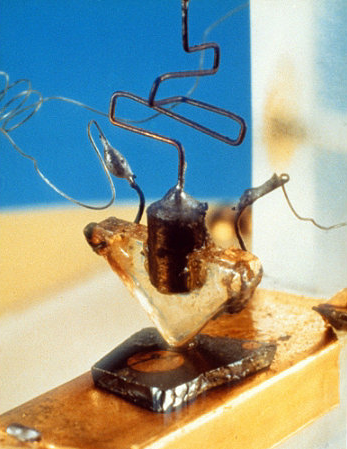
\includegraphics[scale=0.5]{./figures/C02-primer_transistor}
  \captionsetup{justification=centering}
  \caption{Primer transistor desarrollado por John Bardeen y Walter 
    Brattain bajo la dirección de William Shockley en los Laboratorios Bell de 
    AT\&T en el año 1947}.
  \label{fig:C02-primer_transistor}
\end{figure}

\subsection{Silicio, dispositivos semiconductores y transistores}
\label{subsec:theory-history-semiconductors}

Los semiconductores son materiales, que como bien indica su nombre, no son del
todo conductores. En ellos, la capacidad de conducir una corriente eléctrica
puede ser manipulada de diversas maneras. En 1931 Wolfgang Pauli ---quien en 
1945 fue premiado con el Nobel de Física--- enunció: ``Uno no debería trabajar 
en semiconductores, eso es un lío deleznable, quién sabe si realmente existen''.
Nada más alejado de la realidad que hoy nos rodea. Los materiales
semiconductores permitieron la creación de los transistores y posteriormente los
circuitos integrados, dispositivos que iniciaron la revolución digital. Los
primeros dispositivos fueron fabricados sobre germanio y arsenurio de galio.
Incluso, el primer circuito integrado, fue realizado en germanio. Pero fue el 
silicio el material que realmente revolucionó la industria, por su alta
disponibilidad en la naturaleza y relativa fácil manipulación para la
fabricación de dispositivos semiconductores en circuitos integrados. Puede
afirmarse que el silicio es uno de los materiales mejor conocidos por el ser
humano. Hace más de 50 años que se lo estudia en detalle para mejorar la
tecnología, logrando importantes avances. También puede afirmarse que los
transistores hoy en día conforman el bien más abundante en el mundo. Una
comparativa del año 2012 muestra que durante año se produjeron en el órden de
$10^{17}$ granos de arroz en la tierra, mientras que en el mismo período en se
produjeron en el órden de $10^{19}$ transistores, según declaraciones de la
\emph{Semiconductor Industry Asociation} de los Estados Unidos de América. La
clave de semejante número en la producción son los circuitos integrados.

\subsection{Circuitos integrados y tencología CMOS}
\label{subsec:theory-history-ic}

En la figura \ref{fig:C02-primer_circuito_integrado} puede verse el primer
circuito integrado de la historia. Medía aproximadamente media pulgada de ancho
e implementaba dos transistores montados en una barra de germanio. Nace así el
concepto del \emph{chip} o \emph{microchip}: en inglés, \emph{chip} significa
``corte o fracción pequeño de un material duro'' directamente relacionado con la
técnica de fabricación de circuitos integrados donde, a grandes rasgos, una
barra cilíndrica de cristal de silicio puro, es cortada en muy delgadas láminas
en forma de discos, sobre las cuales se ``imprimen'' los circuitos integrados,
repitiendo el mismo patrón múltiples veces en un mismo disco para finalmente
cortar ese disco en diminutos fragmentos que contienen el diseño. La evolución
de las técnicas de fabricación permitieron integrar en un mismo \emph{chip} de
silicio más de un dispositivo, permitiendo implementar circuitos relativamente
complejos en una pequeña área de silicio, disminuyendo así los riesgos de fallas
por interconexión entre dispositivos. A su vez, las técnicas de fabricación
evolucionaron permitiendo escalar el tamaño de los dispositivos fabricados
incrementando la cuenta de dispositivos integrados por unidad de área. Como
consecuencia buscada de disminuir el tamaño de los dispositivos, se logró
aumentar la velocidad máxima de conmutación que los mismos pueden lograr,
redundando en generar lógica cada vez más compleja y rápida en un mismo
\emph{chip}. En simultáneo con estos avances se comenzaron a fabricar
transistores MOSFET\footnote{``Metal-Oxide-Semiconductor Field Effect
Transistor'' (Transistor de efecto de campo Metal-Óxido-Semiconductor): Es un
tipo de transistor fabricado en silicio, donde se genera una estructura que
superpone una capa metálica sobre un óxido sobre material semiconductor,
generando una estructura capacitiva, con la habilidad de manejar la presencia de
un canal conductivo al inducir un campo eléctrico en el material semiconductor.
Éste tipo de transistores presenta diversas ventajas frente a los transistores
bipolares de juntura para el funcionamiento en circuitos digitales.},
transistores de efecto de campo eléctrico, que como gran ventaja sobre los
transistores bipolares de juntura, evitaban la disipación de potencia al
mantenerse en un estado definido (encendido o apagado), es decir que sólo
disipaban potencia al cambiar de estado. Es así que en el año 1978 aparece la
tecnología CMOS\footnote{``CMOS'': técnica de diseño de circuitos lógicos, que
utiliza sólo transistores MOSFET-N y MOSFET-P para implementar cualquier función
lógica.} la cual permitió elevar el nivel de integración en forma masiva,
manteniendo bajos niveles de disipación de potencia. Debido a la relativa
sencillez geométrica del diseño de los transistores MOS, se pueden reutilizar
diseños escalándolos para las nuevas generaciones de tecnología. El 19 de abril
de 1965 Gordon Moore\footnote{Gordon Earle Moore (Nacido el 3 de Enero de 1929):
co-fundador de Intel Corporation, es el autor de la ``Ley de Moore''.},
cofundador de Intel Corporation\footnote{Intel Corporation: fundada el 18 de
Julio de 1968 por Goordon Moore y Robert Noyce, es hoy en día la empresea que
hace punta en el diseño de circuitos integrados y tecnologías de fabricación.
En sus comienzos, su principal negocio fue el desarrollo de circuitos de
memorias SRAM y DRAM, pero a pesar de ser la empresa que creó el primer
microprocesador comercial en 1971, fué luego de la aparición de las ``PC'' que
el diseño de microprocesadores se volvió su principal negocio.}, estableció de
forma empírica que la cantidad de dispositivos integrados en un circuito
integrado se duplicaría cada año. Más tarde, en 1975, modificó su propia ley al
corroborar que el ritmo bajaría, y que la capacidad de integración no se
duplicaría cada 12 meses sino cada 24 meses aproximadamente. Esta progresión de
crecimiento exponencial, duplicar la capacidad de los circuitos integrados cada
dos años, es lo que se denomina ley de Moore. Sin embargo, en 2007 el propio
Moore determinó una fecha de caducidad: ``Mi ley dejará de cumplirse dentro de
10 o 15 años'', no obstante también aseveró que una nueva tecnología vendrá a
suplir a la actual. El cumplimiento se ha podido constatar hasta la actualidad.

\begin{figure}
  \centering
  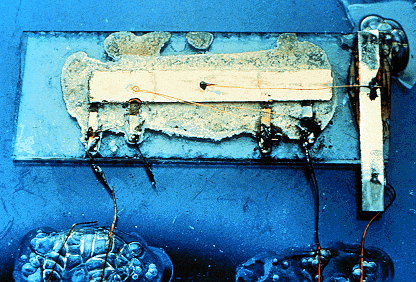
\includegraphics[scale=0.5]{./figures/C02-primer_circuito_integrado}
  \captionsetup{justification=centering}
  \caption{Primer circuito integrado presentado por Texas Instruments, Inc. el 
    12 de Septiembre de 1958}
  \label{fig:C02-primer_circuito_integrado}
\end{figure}

La ley de Moore, no es una ley en el sentido científico, sino más bien una
observación del ritmo de avance de la industria de aquellos momentos. Al momento
de publicar esas declaraciones, Moore trabajaba en los Laboratorios de Fairchild
Semiconductor, donde trabajaba junto a Robert Noyce. Ellos fueron los fundadores
de Intel en 1968. El ritmo de crecimiento de la insdustria de los
semiconductores dió lugar así, entre otras cosas, a la creación de los
microprocesadores.

\subsection{Microprocesadores}
\label{subsec:theory-history-microprocessor}

Los microprocesadores surgen como consecuencia del alto nivel de integración y
complejidad que la tencología de circuitos integrados permitieron alcanzar. Una
computadora digital, podía ser construída en uno o algunos pocos \emph{chips} de
circuitos integrados. Los primeros diseños de microprocesadores propiamente
dichos datan de fines de los años 60. Dentro de este contexto aparece el término
\emph{Central Processing Unit} (Unidad Central de Procesamiento) o CPU, que es
la parte de la máquina encargada de tomar los datos de entrada y las
intrucciones y generar los resultados, dentro del esquema del sistema de
procesamiento planteado al principio de éste capítulo. El microprocesador
integra además otros componentes y funcionalidades y se vale de ciertos
periféricos que pueden estar o no integrados en el mismo circuito, como por
ejemplo, memorias de sólo lectura (\emph{Read Only Memory} o ROM) y memorias de
acceso aleatorio (Random Access Memories o RAM) y dispositivos de
entrada/salida (\emph{I/O, input output devices}. El diseño de arquitecturas de
microprocesarores, como todo proceso de innovación tecnológica, no estuvo exento
de discusiones y distintas vertientes y prácticas a seguir. Los primeros diseños
de los que se tenga registro en órden cronológico, fueron:

\subsubsection{CADC}
\label{subsubsec:theory-history-microprocessor-cadc}

En 1968, la armada de los Estados Unidos de América le encomienda a la empresa
Garret AiResearch\footnote{Garret AiResearch: fundada en 1936 en Los Ángeles por
John Clifford ``Cliff'' Garret, fue una compañía dedicada  al desarrollo de
tecnologías relacionadas a la industria militar aérea.} la producción de una
computadora digital que pudiera competir con los sistemas electromecánicos que
estaban bajo desarrollo para los sistemas de control de vuelo del nuevo avión de
combate F-14 Tomcat. El diseño fue completado en 1970 y utilizaba un conjunto de
chips (\emph{chipset}) MOS como CPU, siendo aproximadamente 20 veces más pequeño
que su contraparte electromecánica y a su vez, mucho más confiable. Este diseño
fue utilizado en todos los primeros modelos de Tomcat. La armada se rehusó a
publicar el diseño hasta 1997, es por eso que la CADC (Central Air Data
Computer) y su \emph{chipset} asociado MP944 no son muy conocidos y no son
considerados en la mayoría de la bibliografía reelevante y es a partir de ese
momento en que son reconocidos como los primeros diseños válidos de
microprocesadores, y no sólo eso, si no que también son la primera especie de
\emph{Digital Signal Processor} (Procesador de Señales Digitales) o
DSP\footnote{``Digital Signal Processor'' (Procesaro de señales digitales): es
un tipo de microprocesador especializado en el tratamiento digital de señales}
puesto que además de las funciones de microprocesador, implementaba la
funcionalidad de medir variables como altitud, velocidad vertical y número de
\emph{mach} a partir de datos de sensores pitot, presión estática y temperatura.
Los responsables del diseño fueron Ray Holt y Steve Geller.

\begin{figure}
  \centering
  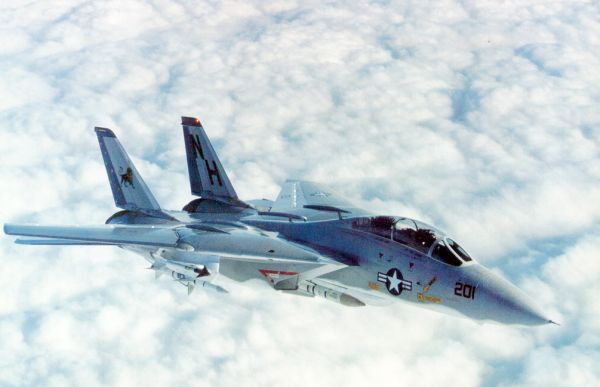
\includegraphics[scale=0.5]{./figures/C02-f14_tomcat}
  \captionsetup{justification=centering}
  \caption{Grumman F14 Tomcat, avión de combate de la US Navy cuyos sistemas de 
    vuelo eran controlados por la CADC.}
  \label{fig:C02-f14_tomcat}
\end{figure}


\subsubsection{Four-Phase Systems AL1}
\label{subsubsec:theory-history-microprocessor-al1}

Un diseño de Lee Boysel que data del año 1969 dentro de Texas
Instruments\footnote{Nota sobre TI}, era un componente de una implementación en
partes de un microprocesador de 24 bits, compuesto por tres chips iguales: AL1.
Durante un juicio por patentes, se demostró que una sóla AL1 junto con memorias
ROM y RAM e I/O era capaz de funcionar como CPU.

\begin{figure}
  \centering
  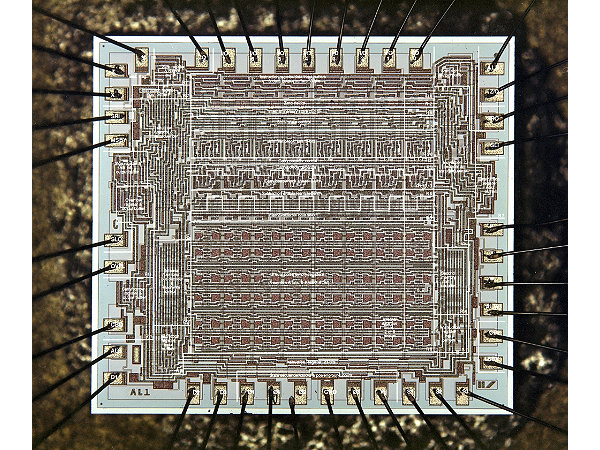
\includegraphics[scale=0.5]{./figures/C02-al1}
  \captionsetup{justification=centering}
  \caption{Imágen microscópica de la AL1 desarrollada por Four-Phase Systems 
    Inc..}
  \label{fig:C02-al1}
\end{figure}


\subsubsection{Pico/General Instruments}
\label{subsubsec:theory-history-microprocessor-pico-gi}

En 1971, Pico y General Instruments (GI) colaboraron en el diseño de circuitos
integrados con el objetivo de fabricar una implementación de un diseño de
\emph{chip} único para la calculadora Monroe/Litton Royal Digital III
Calcultator. Integraba en el mismo \emph{chip}, memoria ROM y RAM llamado
PICO1/GI250. Pico era un emprendimiento de cinco ingenieros de diseño de GI, que
tenían la visión de crear esta arquitectura en un único \emph{chip}. Contaban
con experiencia previa en diseños de \emph{chipsets} tanto de GI como de
Marconi-Elliot. Algunos de ellos habían trabajado para Elliot Automation para
crear una computadora de 8 bits en tecnología MOS, y habían ayudado a establecer
un laboratorio de investigación en tecnologías MOS en Escocia en el año 1967. El
mercado de las calculadoras estaba en pleno auge, con lo cuál estos diseños
supusieron un éxito comercial para Pico y GI. GI, por su parte continuó con la
innovación en microprocesadores  y microcontroladores y la división GI
Microelectronics se convirtió en 1987 en Microchip PIC Microcontroller.

\begin{figure}
  \centering
  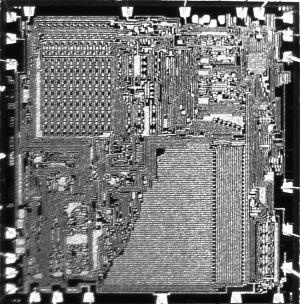
\includegraphics[scale=0.5]{./figures/C02-pico1_gi250}
  \captionsetup{justification=centering}
  \caption{Imágen microscópica del PICO1/GI250- Desarrollo colaborativo entre
    Pico y General Instruments de \emph{chip} único para la Monroe/Litton Royal 
    Digital III Calcultator.}
  \label{fig:C02-pico1_gi250}
\end{figure}

\subsubsection{Intel 4004}
\label{subsubsec:theory-history-microprocessor-4004}

El Intel 4004 es generalmente el reconocido como el primer microprocesador
comercial disponible en el mercado. El primer anuncio respecto de este
dispositivo data del 15 de Noviembre de 1971, en la publicación Electronic News.
El diseño nace a partir del requerimiento de una compañía japonesa fabricante de
calculadoras llamado Busicom, que le encomienda a Intel la tarea de desarrollar
un \emph{chipset} para calculadoras de escritorio de alto rendimiento. El diseño
original requerido por Busicom especificaba un \emph{chipset} compuesto por 7
\emph{chips} diferentes para la realización de una CPU de propósito específico
cuyo programa estuviera almacenado en una ROM y sus datos guardados memoria de
lectura y escritura implementada con registros de desplazamiento. Intel le
asignó el proyecto a Ted Hoff, quien propuso simplificar el diseño utilizando
almacenamiento en memoria RAM dinámica y una arquitectura de CPU de propósito
general. El diseño propuesto por Hoff implementaba la solución en 4
\emph{chips}: uno de ROM para almacenar el programa, uno de RAM dinámica para
almacenar los datos, un dispositivo sencillo de I/O y una CPU de 4 bits. A pesar
de no ser específicamente un diseñador de circuitos integrados, el supuso que se
podía integrar todo el CPU en un único \emph{chip}. Estas especificaciones
surgieron de la interacción de Hoff con un empleado a su cargo, el ingeniero de
software llamado Stanley Mazor y un ingeniero de Busicom llamado Masatoshi
Shima. Este proyecto se llamó MCS-4 y no fué hasta que Intel contratara al
italiano Federico Faggin que empezó a tomar su forma definitiva. Faggin venía de
desarollar en 1968 en Fairchild Semiconductor una teconología de compuertas de
silicio (SGT o \emph{Silicon Gate Technology}), técnica que se sigue aplicando
hoy en día. Faggin también era responsable del desarrollo de la técnica llamada
\emph{Random Logic} que permitió la síntesis de descripciones complejas de
lógica en hardware sencillo, como compuertas AND y OR. En el momento en el que
se estaba desarrollando el proyecto MCS-4, el responsable del área de diseño de
MOS de Intel era Leslie L. Vadász, cuya atención estaba enfocada en el mercado
de memorias. Fue gracias a esto que le otorgó el liderazgo del proyecto MCS-4 a
Faggin, quien fue finalmente el responsable de llevar el proyecto hasta la
concepción final del 4004 gracias a la aplicación de las técnicas de diseño y
fabricación antes mencionadas. Las primeras unidades del 4004 fueron entregadas
a Busicom en Marzo de 1971.

\begin{figure}
  \centering
  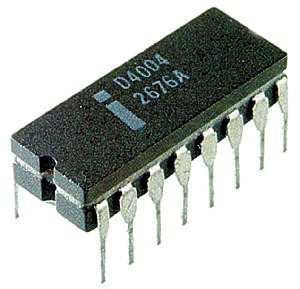
\includegraphics[scale=0.5]{./figures/C02-intel_4004}
  \captionsetup{justification=centering}
  \caption{Encapsulado del Intel 4004; que es considerado el primer
    microprocesador comercial en ser introducido en el mercado.}
  \label{fig:C02-intel_4004}
\end{figure}

\section{Evolución hacia las arquitecturas modernas}
\label{sec:theory-modern}

El concepto moderno de las arquitecturas se basa en las máquinas que almacenan
tanto el programa que se ejecuta, como los datos que se manjan en memoria de
lectura-escritura (\emph{Stored-Program digital computer}). Esto las diferencia
de las primeras implementaciones de los años 40, tales como
Colossus\footnote{Colossus era el nombre de una serie de computadoras
desarrolladas por los británicos para desencriptar las comunicaciones enemigas
durante la segunda guerra mundial. Implementadas con válvulas termoiónicas,
resolvían mediante lógica booleana operaciones de cálculo.} y la ENIAC.\\
En esta sección se estudian las distintas clasificaciones de arquitecturas
existentes hoy en día. Luego se detallarán diversas arquitecturas existentes y
se las enmarcará dentro de dichas clasificaciones.

\subsection{Clasificación de las arquitecturas según el acceso a la memoria de 
instrucciones y datos}
\label{subsec:theory-modern-memory_access}

Las instrucciones que ejecuta el procesador, al igual que los datos del programa
en ejecución, deben residir en la memoria. De este hecho se desprende que
existen ---al menos--- dos tipos de memorias: de instrucciones, y de datos. El
acceso a estas dos memorias puede realizarse a través del mismo
\emph{bus}\footnote{Bus: definir bus} o con \emph{buses} separados. Los nombres
que la historia les ha provisto a estos dos posibles enfoques, son
\emph{von Neumann} para las arquitecturas de \emph{bus} único y \emph{Harvard}
para aquellas de \emph{buses} separados.

\subsubsection{Arquitectura von Neumann}
\label{subsubsec:theory-modern-memory_access-von_neumann}

También conocida como modelo de von Neumann y arquitectura Princeton, este tipo
de arquitectura debe su nombre a John von Neumann\footnote{Nota sobre el
chango}, quién en el año 1945 describió en el documento inconcluso, cuya
carátula puede verse en la figura \ref{fig:C02-von_neumann_first_draft} y
conocido como \emph{First Draft of a Report on the EDVAC}\cite{vonNeumann}, una
arquitectura de computadora electrónica digital para ser implementada con
válvulas de vacío. Ésta fue la primera publicación dónde se describe el diseño
lógico de una computadora que utilizase el concepto de \emph{stored-program} o
programa almacenado. Este diseño, tal como fue llamado por el propio von
Neumann, \emph{very high speed automatic digital computing system} o sistema
automático digital de cómputo de muy alta velocidad, estaba dividido en 6
componentes:
\begin{itemize}
  \item CA: \emph{central arithmetic} o aritmética central
  \item CC: \emph{central control} o control central
  \item M: \emph{memory} o memoria
  \item I: \emph{input} o entrada
  \item O: \emph{output} o salida
  \item R: \emph{external memory} o memoria externa
\end{itemize}
\begin{figure}
  \centering
  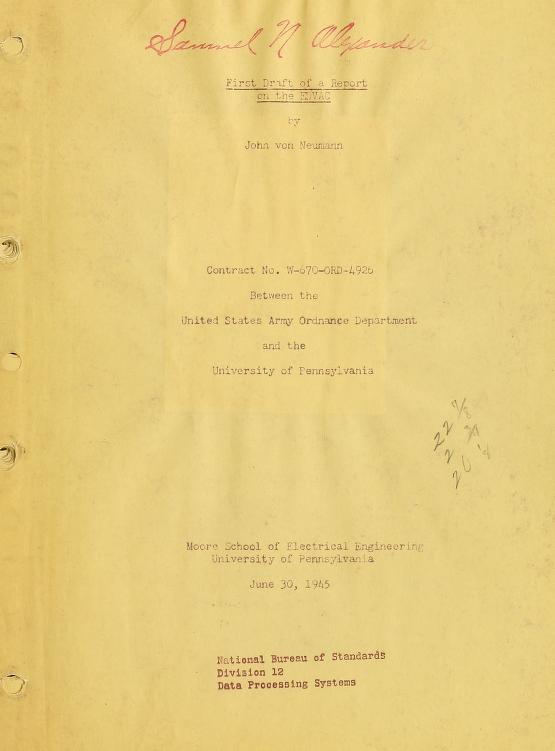
\includegraphics[scale=0.25]{./figures/C02-von_neumann_first_draft}
  \captionsetup{justification=centering}
  \caption{Carátula del escrito de von Neumann First Draft of a Report on the EDVAC}
  \label{fig:C02-von_neumann_first_draft}
\end{figure}
La memoria almacena tanto números (datos) como órdenes (instrucciones).
La aritmética central podía realizar sumas, restas, multiplicaciones, divisiones
y raices cuadradas. Otras operaciones matemáticas, como logaritmos y funciones
trigonométricas se debían realizar utilizando tablas de búsqueda e
interpolaciones, posiblemente bicuadráticas. Una decisión de diseño establecida
en el documento estableció que multiplicaciones y divisiones podían realizarse
mediante tablas logarítmicas, pero para poder mantener dichas tablas pequeñas
debería utilizarse interpolaciones, lo cuál a su vez necesita de
multiplicaciones, aunque de menor precisión.\\
Los números se represetaban mediante notación binaria. Estimó que 27 dígitos
binarios\footnote{En el documento se hace meción a dígitos binarios y no a
\emph{bits}, término que fue acuñado en 1948 por Claude Shannon} deberían ser
suficientes, pero redondéo a 30 dígitos, más uno de signo y otro para
diferenciar los números de las órdenes, resultando en palabras de 32 dígitos
binarios. La aritmética utilizada era complemento a dos para simplificar la
operación de resta. Para la multiplicación y la división, propuso ubicar el
punto binario luego del bit de signo, lo que implica que el dominio de los
operandos y resultados está en el rango -1 a 1, y por lo tanto, los datos y
resultados de los programas deberían ser escalados acordemente.\\
En cuanto al diseño de los circuitos, estableció que deberían utilizarse
válvulas de vacío, dejando de lado los relé, dada a la mayor velocidad provista
por las primeras. Otras sugerencias involucraban mantener al sistema de cómputo
lo más sencillo posible, evitando cualquier tipo de optimización de performance
mediante la superposición de operaciones. Las operaciones aritméticas debían
realizarse de a un dígito binario a la vez. Estimó el tiempo de la suma de dos
dígitos binarios en un microsegundo, por lo tanto la multiplicación de dos
números representados por 30 dígitos binarios deberí realizarse en
aproximadamente $30^{20}$ microsegundos; lo cuál era mucho más rápido que el
tiempo de cualquier dispositivo de cálculo del momento. El diseño estaba basado
en lo que von Neumann llamó ``elemento E'', basándose en el modelo biológico de
las neuronas, pero implementado de forma digital planteando que podrían ser
fabricados mediante una o dos válvulas. En términos modernos, la forma más
sencilla del ``elemento E'' es una compuerta \emph{AND} de dos entradas, con una
de sus entradas invertidas, llamada ``entrada de inhibición''. Al agregar más
entradas a este dispositivo, se establecía un nivel de umbral, el cual al ser
superado por la suma de una determinada cantidad de entradas generaba una salida
en tanto y en cuanto no se excitara la entrada de inhibición. También estableció
que dichos elementos de múltiples entradas podían ser construidos utilizando
combinaciones de la versión elemental, pero recomendaba implementarlos por
completo utilizando así menos válvulas de vacío con el objetivo de lograr
circuitos más sencillos y rápidos, principio que hoy en día se mantiene
vigente.\\
Toda función lógica arbitraria, podía implentarse, entonces, a partir de dichos
``elementos E''. Demostró en este trabajo, cómo implementar circuitos que
implementaban las funciones aritméticas, así como elementos de memoria y
circuitos de control, sin referirse en ningún momento al término de ``lógica
binaria''.\\
Los ciruitos debían ser sincrónicos, obteniendo la señal de reloj a partir de un
circuito oscilador implementado con válvulas y posiblemente controlado mediante
cristales osciladores. Los diagramas lógicos incluían los tiempos de demora
representados mediante una flecha. Estimó que la velocidad a la que se movía un
pulso eléctrico en un cable era de $300 mts/microsegundo$, por lo tanto no
debería generar problemas hasta obtener velocidades de reloj de $100MHz$.
Tambíen menciona pero no desarrolla la necesidad de contar con mecanismos de
detección y correción.\\
En cuanto a la memoria, que es donde entra la clasificación discutida en esta
sección, von Neumann estableció que la memoria es uniforme, conteniendo tanto
los números (datos) como las órdenes (instrucciones). Citando su trabajo:
\begin{quote}
  El dispositivo requiere una memoria considerable. A pesar de que pareciese 
  que distintas partes de la memoria tiene que realizar funciones que difieren 
  en su naturaleza y considerablemente en su propósito, resulta tentador tratar 
  a toda la memoria con un sólo órgano, y hacer que sus partes sean tan 
  intercambiables como sea posible para todas las funciones que deban realizar. 
  \cite[sección, 2.5]{vonNeumann}
\end{quote}
\begin{quote}
  Lás órdenes recibidas por CC vienen de M, es decir, el mismo lugar donde se
  almacenan los datos numéricos.\cite[sección, 14.0]{vonNeumann}.
\end{quote}
Él concluyó que la memoria sería el subsistema más grande y abarcativo de la
máquina. Basándose en diversos problemas matemáticos, incluyendo la resolución
de ecuaciones diferenciales parciales y ordinarias, ordenamientos y experimentos
probabilísticos, estimó que se necesitaba espacio para almacenar 8192 palabras
de 32 dígitos binarios para los datos, y algunos cientos de palabras para
almacenar las órdenes. Para la implementación de memoria, propuso dos tipos de
memoria rápida, \emph{delay line memory} e \emph{iconoscope}. Con estas
implementaciones planteó que la memoria debía ser direccionable por palabras y
para sortear los problemas de demora asociados a la lectura de estas memorias,
organizó las mismas en 256 conjuntos de 1024 dígitos binarios, o sea 32
palabras, logrando así direccionar los conjuntos con 8 dígitos binarios y las
palabras con 5 utilizando, entonces, 13 dígitos binarios en total para el
direccionamiento completo.\\
En su trabajo también estableció el formato de las órdenes, al cual llamó
``código''. Los tipos de órdenes incuyeron las operaciones aritméticas básicas,
así como el movimiento de palabras entre CA y M (análogas a las instrucciones
\emph{load} y \emph{store} de hoy en día que veremos más adelante), una órden
que elegía entre dos números basado en el signo del resultado de una operación
previa (análoga a una instrucción \emph{branch}), órdenes para controlar la
entrada y salida de datos y para indicarle a la CC que debía tomar instrucciones
desde otra sección de M (análoga a un \emph{jump}). Determinó, asimismo, la
cantidad de dígitos binarios necesarios para necesarios para los distintos tipos
de órdenes, sugirió lo que llamó ``órdenes inmediatas'', donde la siguiente
palabra  se trata del operando (lo cual también tiene una anagolía con ciertos
conjuntos de instrucciones actuales) y dejó planteado si era deseable dejar
dígitos sin especificar para propósitos futuros y mayor direccionamiento de
memoria.

\subsubsection{Arquitectura Harvard}
\label{subsubsec:theory-modern-memory_access-harvard}

Este tipo de arquitectura, ve sus orígenes en un desarrollo propuesto por el Dr.
Howard Aiken\footnote{Nota sobre Aiken} en la universidad de Harvard en el año
1937 basado en el trabajo llamado \emph{Analytical Engine}\footnote{Nota sobre
Analytical Engine} de Charles Babage\footnote{Nota sobre el tipo}. El desarrollo
fue llevado al cabo por IBM\footnote{Nota sobre IBM} y se trataba de una máquina
de cálculo llamada \emph{Automatic Sequence Controlled Calculator - Harvard Mark
I} entregado a la universidad el 24 de agosto de 1944. A diferencia de la
máquina propuesta (posteriormente) por von Neumann, ésta era una máquina
electromecánica construida con llaves, relés, engranajes y embreagues. Constaba
de 765000 componentes electromecánicos, cientos de millas de cableado, un peso
de 4.5 Ton. y un consumo de potencia de 3.7 kW. Para el ingreso de datos,
contaba con 60 conjuntos de 24 llaves rotativas que permitían ingresar números
decimales. Podía almacenar hast 72 números de hasta 23 dígitos decimales. En un
segundo era capaz de realizar 3 sumas o restas. La multiplicación tardaba 6
segundos y una división 13.5 segundos. El calculo de funciones logarítmicas o
trigonométricas utilizaba más de un minuto. Las instrucciones eran ingresadas a
través de cintas perforadas de 24 canales (en la figura
\ref{fig:C02-mark_i_instruction_tape} se puede ver una cinta con instrucciones
de esta máquina). Otra cinta podía ser utilizada para el ingreso de datos, pero
utilizando un formato distinto al de las instrucciones; estas no podían ser
ejecutadas desde los registros de almacenamiento. Esta separación entre datos e
instrucciones es lo que se conoce como arquitectura Harvard y que la diferencia
de la arquitectura von Neumann. El formato de las instrucciones definía tres
campos en ocho canales separados. Cada acumulador, cada conjunto de switches, y
los registros asociados a la entrada y salida y las unidades aritméticas tenían
asignado un índice único. Estos números eran representados en formato binario en
la cinta perforada de control, siendo el primer campo el índice del resultado de
la operación, el segundo el orígen del dato para la operación y el tercero el
código que representa la operación a realizar. Una particularidad de ésta
primera versión es que no tenía instrucción para el salto condicional en el
programa. Por lo tanto, los programas complejos debían ser largos y los
``loops'' se implementaban uniendo físicamente el final de la cinta perforada
del programa con el principio.\\
\begin{figure}
  \centering
  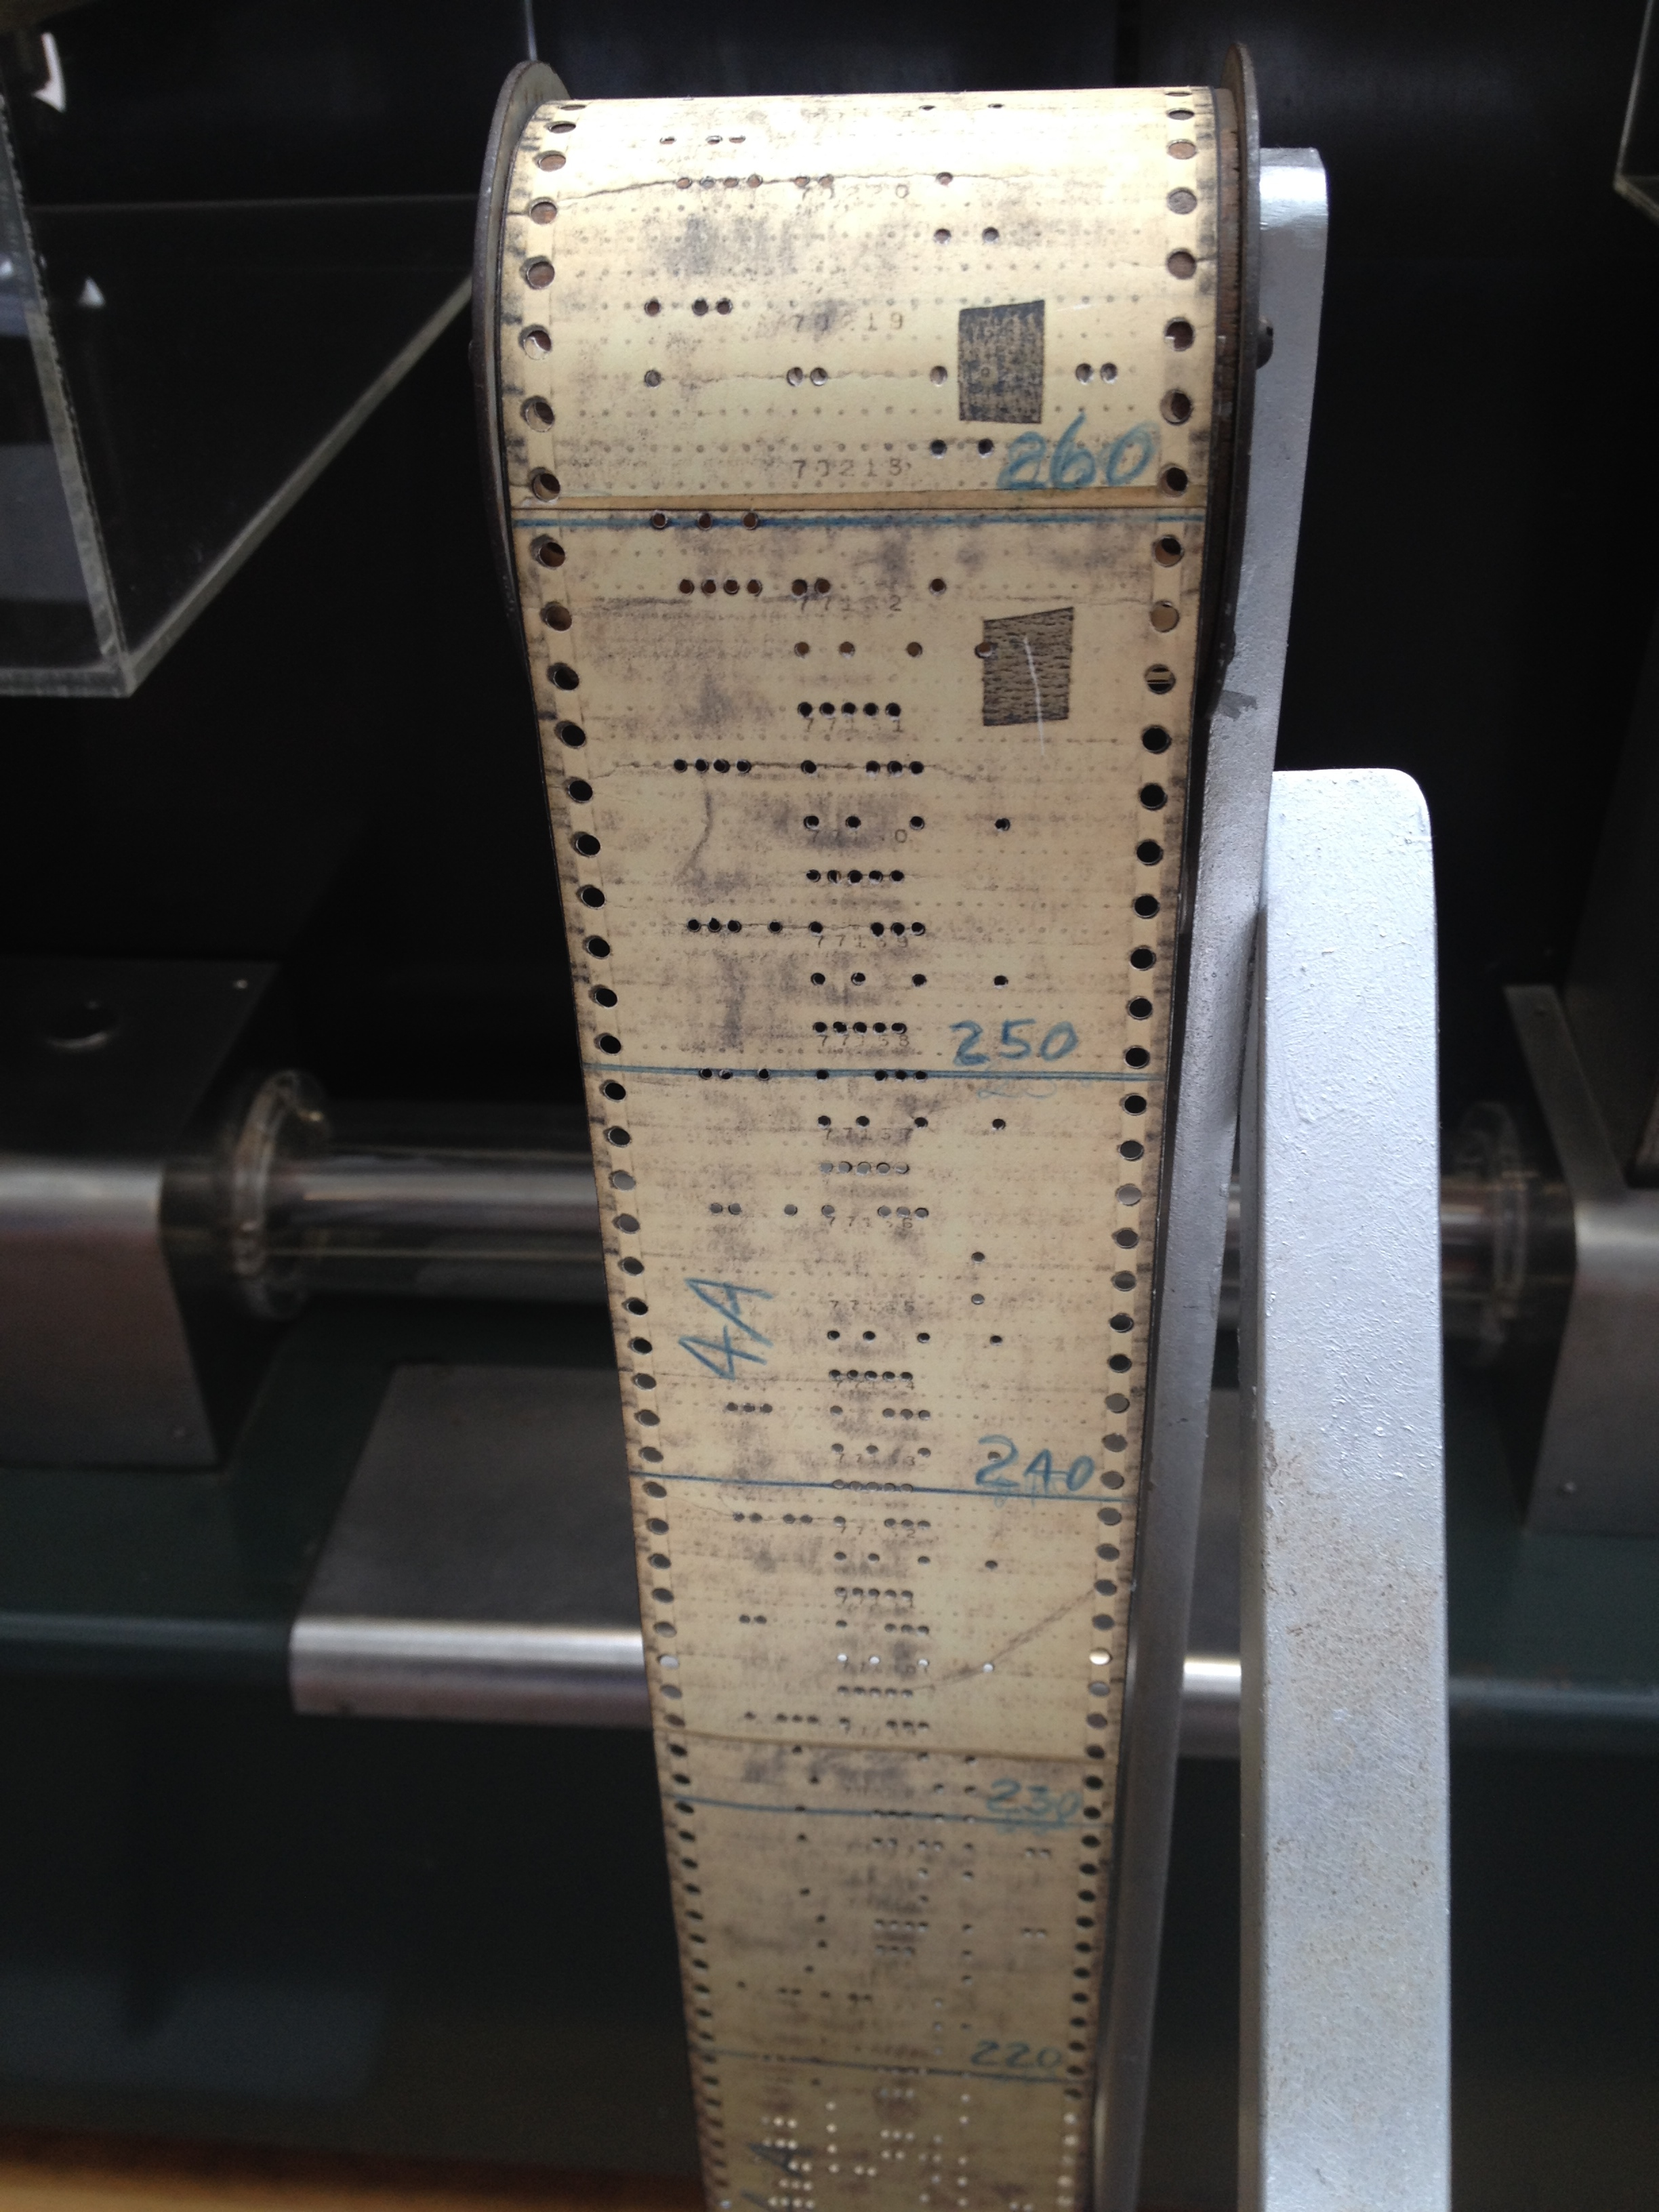
\includegraphics[scale=0.05]{./figures/C02-mark_i_instruction_tape}
  \captionsetup{justification=centering}
  \caption{Cinta de papel perforado con instrucciones de la Mark I}
  \label{fig:C02-mark_i_instruction_tape}
\end{figure}
La Mark I fue sucedida por la Mark II en el año 1948, la Mark III en septiembre
de 1949 y la Mark IV en el año 1952, todos estos proyectos fueron de Aiken. La
Mark II fue una mejora sobre la Mark I, pero aún basada en componentes
electromecánicos. La tercer versión utilizaba en su mayoría componentes
electrónicos tales como válvulas de vacío y diodos cristalinos, pero utilizaba
cilindros magnéticos para almacenamiento, y relés para la transferencia de datos
entre ellos. La cuarta versión fue la primera en ser completamente electrónica,
reemplazando los cilindros magnéticos de almacenamiento con memorias de núcle
magnético; el tipo de memoria de acceso aleatorio predominante entre 1955 y
1975.

\subsubsection{Harvard vs. von Neumann y Harvard modificada}
\label{subsubsec:theory-modern-memory_access-modified_harvard}

Como fue establecido al principio de esta sección, lo que diferencia estas dos
arquitecturas es el acceso a los datos y a las instrucciones. La arquitectura
von Neumann puede tratar a los datos como instrucciones y viceversa, dado que
para dicha arquitectura, la memoria es exactamente la misma, con el mismo tipo
de acceso y el mismo direccionamiento, contrariamente a lo que es una
arquitectura puramente Harvard, cuyas memorias de datos e instrucciones se
acceden por diferentes medios y cuyas direcciones pueden estar sobrepuestas (es
decir que la misma dirección de memoria no representa lo mismo si se trata de
datos o intrucciones) y por lo tanto, los datos y las intrucciones no pueden ser
intercambiados en el tratamiento que se realiza dentro de la unidad de cómputo.
Dadas estas condiciones, las principales desventajas son que, la arquitectura
von Neumann no puede acceder simultáneamente a datos y a instrucciones y la
máquina de Harvard no puede ni leer ni escribir en el espacio de memoria de las
instrucciones, denegando por lo tanto cualquier posibilidad de código
auto-optimizable o inteligente que reescriba sus instrucciones, así como tambíen
la carga de los programas a partir de medios de almacenamiento de datos.\\
Hoy en día, las máquinas puramente Harvard no son más que una especialidad.
Típicamente, en las máquinas modernas, se implementas arquitecturas Harvard
modificadas. Estas modificaciones pueden ser de diversos tipos:

\paragraph{Arquitectura de caché separado}
\label{par:theory-modern-memory_access-modified_harvard-split_cache}

Es la modificación más común sobre la arquitectura Harvard, se construye una
jerarquía de memoria donde el nivel más cercano al núcleo de procesamiento
(típicamente llamado caché de nivel 1) está separado en datos e instrucciones, y
unificando estas memorias en un nivel de jerarquía superior. Con esta técnia, se
puede relajar el problema de acceder a la memoria de instrucciones como datos,
tanto para la lectura como para la escritura al unificar toda la memoria en un
solo espacio de direccionamiento, emulando así el comportamiento de una
arquitectura de von Neumann, pero manteniendo la ventaja de poder acceder a
datos e instrucciones de forma simultánea. Esta característica será transparente
para la mayoría de los programadores, excepto aquellos casos en los que es
necesario el manejo de técnicas como por ejemplo, la coherencia de caches.

\paragraph{Acesso a instrucciones como datos}
\label{par:theory-modern-memory_access-modified_harvard-instructions_as_data}

Un arquitectura que provea esta solución matiene la naturaleza de espacios de
direcciones separados de la arquitectura Harvard, pero incluye operaciones
especializadas en acceder al contenido de la memoria de instrucciones como si
fueran datos. Como los datos no pueden ser ejecutados driectamente como
instrucciones, estas implementaciones no siempre son vistas como Harvard
``modificadas''.\\
Esta técnica puede presentarse con dos variantes. Por un lado, el acceso puede
ser de sólo lectura, provee la capacidad de copiar contenido embebido en el
código cargado en la memoria de instrucciones a la memoria de datos cuando el
programa comienza o, mejor aún, si los datos no van a cambiar (como es el caso
de constantes aritméticas o cadenas de texto predefinidas), estos datos que
están en la memoria de instrucciones pueden ser directamente leídos en tiempo de
ejecución por el programa sin tomar espacio de la memoria de datos (que puede
ser escasa en las implementaciones que aplican esta técnica). Por otro lado,
dicho acceso puede ser de lectura/escritura, suele darse cuando es necesaria una
capacidad de reprogramación de la máquina en cuestión. Pocas computadoras hoy en
día están basadas únicamente en ROM para su funcionamiento. Puede ser el caso de
algunos microcontroladores que tienen operaciones para escribir en su memoria
``Flash'' (en la cual se almacenan las instrucciones). Esta capacidad provee
medios de acceso para actualizaciones de software/firmware y reemplaza a las
EEPROM.

\paragraph{Ejecución de datos}
\label{par:theory-modern-memory_access-modified_harvard-data_execution}

Algunas arquitecturas pueden obtener sus instrucciones desde cualquier segmento
de memoria con la limitación de que no podrá acceder simultáneamente para leer
instrucciones y datos de un mismo segmento de memoria. Para lograr este
comportamiento, se direccionan los buses tanto de datos como de instrucciones
sobre distintos segmentos físicos de una misma memoria.

\paragraph{Características de las arquitecturas Harvard modificadas}
\label{par:theory-modern-memory_access-modified_harvard-characteristitcs}

Tres características pueden ser utilizadas para diferenciar a este tipo de
arquitectura de las Harvard puras y de las von Neumann:\\

\subparagraph{Las memorias de datos e instrucciones ocupan diferentes espacios
de direccionamiento}
\label{subpar:theory-modern-memory_access-modified_harvard-characteristitcs-1}

Para las máquinas puramente Harvard, hay una dirección ``cero'' de instrucciones
en el espacio de direcciones de las instrucciones y una dirección ``cero'' de
datos en el espacio de direcciones de los datos que referencian a un lugares de
almacenamiento distintos. En contraste, las máquinas von Neumann y algunas
Harvard modificadas (como las de caché separado), almacenan tanto datos como
instrucciones en un espacio de direcciones unificado, por lo tanto, la dirección
``cero'' hace referencia a una sóla cosa y lo almacenado allí puede ser la
representación binaria de un código de instrucción o de un dato, dependiendo de
cómo fue escrito el programa en ejecución. Sin embargo, tal como las máquinas
puramente Harvard, las Harvard modificadas con espacios de direcciones
separados, pero con instrucciones específicas que permiten leer y escribir las
instrucciones como datos, tienen una direcciónes solapadas para los respectivos
espacios de direccionamiento, por lo tanto esto no distingue las máquinas
puramente Harvard de este último tipo de Harvard modificadas.

\subparagraph{Las memorias de datos e instrucciones tienen conexiones físicas
separadas hacia el núcleo de procesamiento}
\label{subpar:theory-modern-memory_access-modified_harvard-characteristitcs-2}

Este es el motivo principal por el que existen las arquitecturas Harvard (tanto
puras como modificadas), y por qué coexisten con las más generales y flexibles
von Neumann: los caminos separados físicamente para los datos y las
instrucciones permiten que las instrucciones sean cargadas en la unidad de
cómputo al mismo tiempo que los datos, aumentando así el rendimiento. Las
máquinas puramente Harvard tienen caminos separados con espacios de direcciones
separados. Las máquinas de caché separado proveen este acceso separado para la
unidad de procesamiento pero presentan un espacio de direccionamiento unificado
al ascender en la jerarquía de memoria. Una máquina von Neumann puede tenera
sólamente un espacio de direcciones unificado. Para el punto de vista del
programador, una arquitectura de cache separado es tratada de forma equivalente
a una von Neumann (al menos hasta el punto en el que el tratamiendo de
coherencia de cache se convierta en significativo), como puede ser el caso de
código auto-optimizable o la carga de un programa en memoria desde un medio de
almacenamiento externo. Otras arquitecturas Harvard modificadas se comportan
como Harvard puras en este ámbito.

\subparagraph{Las memorias de datos e instrucciones pueden ser accedidas de
diferentes formas}
\label{subpar:theory-modern-memory_access-modified_harvard-characteristitcs-3}

Las máquinas Harvard puras, al tener distintos espacios de memoria para datos e
instrucciones, pueden acceder a dichas memorias de distintas maneras. Puede ser
el caso de una arquitectura donde la memoria de instrucciones se direccione con
una cantidad de bits distinta a la de datos. Esto no es posible en una
arquitectura von Neumann ni en una Harvard modificada de cache separado, dado
que ambos espacios de memoria deben estar superpuestos.

\subsubsection{Aplicaciones de esta clasificación en la actualidad}
\label{subsubsec:theory-modern-memory_access-current_aplications}

En áreas específicas donde un memoria cache es prohibitiva (puede ser el caso de
los DSP por el determinismo necesario para las diversas operaciones, o de
microcontroladores por el bajo costo), pueden darse arquitecturas Harvard puras
o von Neumann. En modelos donde el uso es de propósito general, típicamente se
utilizan arquitecturas Harvard modificadas con caché separado debido a que tener
espacios de direccionamiento separados genera dificultados con ciertos lenguajes
de programación de alto nivel que no soportan la noción de tener datos de sólo
lectura cargados en un espacio de direccionamiento distinto al de los datos
comunes, con la necesidad de utilizar distintas instrucciones para leerlos. El
lenguaje de programación ``C'' soporta este comportamiento a través de
extensiones propietarias, aunque hoy en día ya existen estandarizaciones para
los llamados procesares embebidos.

\subsection{Taxonomía de Flynn}
\label{subsec:theory-modern-flynn_taxonomy}

La taxonomía de Flynn es una clasificación de las arquitecturas basada en la 
cantidad de ``hilos'' de control y de datos que soporta el 
procesador de forma concurrente. Establecida en 1966 por Michael 
Flynn\footnote{Michael J. Flynn (Nacido el 20 de Mayo de 1934): es un profesor 
emérito de la universidad de Stanford que propuso la llamada ``Taxonomía de 
Flynn'' para clasificar las arquitecturas de computadoras en el año 1966}, 
estableciendo los efectos que pueden surgir de explotar el paralelismo tanto en 
los hilos de instrucciones como en los de datos. Se puede tener hilos únicos o 
múltiples para cada uno de ellos. Es estas definiciones, Flynn estableció que 
una máquina identifica los siguientes conceptos:
\begin{itemize}
  \item CU: \emph{contro unit} o unidad de control
  \item PE: \emph{processing element} o elemento de procesamiento
  \item IS: \emph{instruction stream} o hilo de instrucciones
  \item DS: \emph{data stream} o hilo de datos  
\end{itemize}
Al combinar hilos sencillos y múltiples de datos e instrucciones se da lugar, 
entonces, a cuatro tipo de arquitecturas (ver tabla \ref{tbl:flynn_taxonomy}).
\begin{table}
  \begin{tabu} to \textwidth {X[l]cc}
    \toprule
				& Hilo simple de instrucciones	& Hilo múltiple 
de instrucciones\\
    \midrule
    Hilo simple de datos	& SISD				& MISD\\
    Hilo múltiple de datos	& SIMD				& MIMD\\
    \bottomrule
  \end{tabu}
  \caption{Taxonomía de Flynn}
  \label{tbl:flynn_taxonomy}
\end{table}

\subsubsection{SISD: Simple Instruction stream, Simple Data stream}
\label{subsubsec:theory-modern-flynn_taxonomy-SISD}

Resultante de combinar un único hilo de control con un único hilo de datos, 
este tipo de arquitectura no explota ningún paralelismo en una máquina 
completamente secuencial. Una única CU obtiene un único IS de 
memoria. La CU genera las señales de control necesarias para excitar a un 
único PE sobre un único DS, es decir, una operación a la vez. Ver figura 
\ref{subfig:sisd}.\\
Un ejemplo de esta arquitectura son los procesadores de las antiguas 
computadoras personales.

\subsubsection{SIMD: Simple Instruction stream, Multiple Data stream}
\label{subsubsec:theory-modern-flynn_taxonomy-SIMD}

En este tipo de arquitecturas, sige existiendo un único hilo de control, pero 
los datos que afectan las instrucciones provienen de distintos hilos de datos. 
La CU trabaja con las instrucciones de un único IS y general las señales de 
control necesarias para que mútiples PE procesen los datos provenientes de 
múltiples DS. Es un tipo de máquina que es naturalmente paralelizable. Ver 
figura \ref{subfig:simd}.\\
Ejemplos de este tipo de arquitecturas son los procesadores matriciales y las 
unidades de procesamiento gráficas (GPU). Cabe destacar que los antiguos 
procesadores de PC, en un determinado momento incorporaron instrucciones 
específicas con el que lograban este comportamiento, tales como las extensiones 
multimedia (MMX) que Intel incluyó en su línea de procesadores Pentium a 
mediados de los años '90.

\subsubsection{MISD: Múltiple Instruction stream, Simple Data stream}
\label{subsubsec:theory-modern-flynn_taxonomy-MISD}

Se trata de arquitecturas en el que diversos hilos de control actuan sobre un 
único hilo de datos. No se trata de un tipo común de arquitecturas, si no más 
bien de un tipo específico utilizado en sistemas tolerantes a fallas. Diversos 
sistemas heterogéneos operan sobre el mismo hilo de datos y deben arribar al 
mismo resultado. Es decir que diversas CU toman instrucciones de diversos IS 
controlando múltiples PE que actuan sobre un único DS. Ver figura 
\ref{subfig:misd}.\\
Ejemplos de este tipo de máquinas pueden ser las computadoras de control de 
vuelo de aeronaves y naves espaciales o cohetes; es decir aplicaciones de 
misión crítica que poseen sistemas redundantes y decisores.

\subsubsection{MIMD: Multiple Instruction stream, Multiple Data stream}
\label{subsubsec:theory-modern-flynn_taxonomy-MIMD}

Se trata de arquitecturas donde múltiples procesadores simultáneamente ejecutan 
diversos hilos de instrucciones sobre diversos hilos de datos. Es decir que 
diversas CU toman instrucciones de diversos IS para excitar a diversos PE que 
actúan sobre diversos DS. Ver figura \ref{subfig:mimd}.\\
Los procesadores multinúcleo y los sistemas distribuidos son ejemplos de éste 
tipo de máquinas, y pueden utilizar tanto un espacio de memoria compartido, así 
como uno distribuído.
% TODO: Revisar por qué las últimas dos figuras no quedan bien armadas.
\begin{figure}
  \begin{subfigure}[b]{0.5\textwidth}
    % Graphic for TeX using PGF
% Title: /home/lnatale/Documents/xfire/digital/xfire_core/docs/thesis/tesis/figures/C02-sisd.dia
% Creator: Dia v0.97.3
% CreationDate: Sat Jul 23 17:44:13 2016
% For: lnatale
% \usepackage{tikz}
% The following commands are not supported in PSTricks at present
% We define them conditionally, so when they are implemented,
% this pgf file will use them.
\ifx\du\undefined
  \newlength{\du}
\fi
\setlength{\du}{15\unitlength}
\begin{tikzpicture}
\pgftransformxscale{1.000000}
\pgftransformyscale{-1.000000}
\definecolor{dialinecolor}{rgb}{0.000000, 0.000000, 0.000000}
\pgfsetstrokecolor{dialinecolor}
\definecolor{dialinecolor}{rgb}{1.000000, 1.000000, 1.000000}
\pgfsetfillcolor{dialinecolor}
\definecolor{dialinecolor}{rgb}{1.000000, 1.000000, 1.000000}
\pgfsetfillcolor{dialinecolor}
\fill (3.000000\du,2.000000\du)--(3.000000\du,4.000000\du)--(12.000000\du,4.000000\du)--(12.000000\du,2.000000\du)--cycle;
\pgfsetlinewidth{0.100000\du}
\pgfsetdash{}{0pt}
\pgfsetdash{}{0pt}
\pgfsetmiterjoin
\definecolor{dialinecolor}{rgb}{0.000000, 0.000000, 0.000000}
\pgfsetstrokecolor{dialinecolor}
\draw (3.000000\du,2.000000\du)--(3.000000\du,4.000000\du)--(12.000000\du,4.000000\du)--(12.000000\du,2.000000\du)--cycle;
% setfont left to latex
\definecolor{dialinecolor}{rgb}{0.000000, 0.000000, 0.000000}
\pgfsetstrokecolor{dialinecolor}
\node at (7.500000\du,3.195000\du){IS};
\definecolor{dialinecolor}{rgb}{1.000000, 1.000000, 1.000000}
\pgfsetfillcolor{dialinecolor}
\fill (0.000000\du,5.000000\du)--(0.000000\du,14.000000\du)--(2.000000\du,14.000000\du)--(2.000000\du,5.000000\du)--cycle;
\pgfsetlinewidth{0.100000\du}
\pgfsetdash{}{0pt}
\pgfsetdash{}{0pt}
\pgfsetmiterjoin
\definecolor{dialinecolor}{rgb}{0.000000, 0.000000, 0.000000}
\pgfsetstrokecolor{dialinecolor}
\draw (0.000000\du,5.000000\du)--(0.000000\du,14.000000\du)--(2.000000\du,14.000000\du)--(2.000000\du,5.000000\du)--cycle;
% setfont left to latex
\definecolor{dialinecolor}{rgb}{0.000000, 0.000000, 0.000000}
\pgfsetstrokecolor{dialinecolor}
\node at (1.000000\du,9.695000\du){DS};
% setfont left to latex
\definecolor{dialinecolor}{rgb}{0.000000, 0.000000, 0.000000}
\pgfsetstrokecolor{dialinecolor}
\node[anchor=west] at (1.000000\du,9.500000\du){};
% setfont left to latex
\definecolor{dialinecolor}{rgb}{0.000000, 0.000000, 0.000000}
\pgfsetstrokecolor{dialinecolor}
\node[anchor=west] at (7.500000\du,3.000000\du){};
\definecolor{dialinecolor}{rgb}{1.000000, 1.000000, 1.000000}
\pgfsetfillcolor{dialinecolor}
\fill (4.000000\du,8.000000\du)--(4.000000\du,11.000000\du)--(5.952500\du,11.000000\du)--(5.952500\du,8.000000\du)--cycle;
\pgfsetlinewidth{0.100000\du}
\pgfsetdash{}{0pt}
\pgfsetdash{}{0pt}
\pgfsetmiterjoin
\definecolor{dialinecolor}{rgb}{0.000000, 0.000000, 0.000000}
\pgfsetstrokecolor{dialinecolor}
\draw (4.000000\du,8.000000\du)--(4.000000\du,11.000000\du)--(5.952500\du,11.000000\du)--(5.952500\du,8.000000\du)--cycle;
% setfont left to latex
\definecolor{dialinecolor}{rgb}{0.000000, 0.000000, 0.000000}
\pgfsetstrokecolor{dialinecolor}
\node at (4.976250\du,9.695000\du){PE};
\pgfsetlinewidth{0.100000\du}
\pgfsetdash{}{0pt}
\pgfsetdash{}{0pt}
\pgfsetbuttcap
{
\definecolor{dialinecolor}{rgb}{0.000000, 0.000000, 0.000000}
\pgfsetfillcolor{dialinecolor}
% was here!!!
\pgfsetarrowsend{latex}
\definecolor{dialinecolor}{rgb}{0.000000, 0.000000, 0.000000}
\pgfsetstrokecolor{dialinecolor}
\draw (2.000000\du,9.500000\du)--(4.000000\du,9.500000\du);
}
\pgfsetlinewidth{0.100000\du}
\pgfsetdash{}{0pt}
\pgfsetdash{}{0pt}
\pgfsetmiterjoin
\pgfsetbuttcap
{
\definecolor{dialinecolor}{rgb}{0.000000, 0.000000, 0.000000}
\pgfsetfillcolor{dialinecolor}
% was here!!!
\pgfsetarrowsend{latex}
{\pgfsetcornersarced{\pgfpoint{0.000000\du}{0.000000\du}}\definecolor{dialinecolor}{rgb}{0.000000, 0.000000, 0.000000}
\pgfsetstrokecolor{dialinecolor}
\draw (7.500000\du,4.000000\du)--(10.000000\du,4.000000\du)--(10.000000\du,9.500000\du)--(5.952500\du,9.500000\du);
}}
% setfont left to latex
\definecolor{dialinecolor}{rgb}{0.000000, 0.000000, 0.000000}
\pgfsetstrokecolor{dialinecolor}
\node[anchor=west] at (4.976250\du,9.500000\du){};
\end{tikzpicture}

    \caption{SISD}
    \label{subfig:sisd}
  \end{subfigure}
  \begin{subfigure}[b]{0.5\textwidth}
    % Graphic for TeX using PGF
% Title: /home/lnatale/Documents/xfire/digital/xfire_core/docs/thesis/tesis/figures/C02-simd.dia
% Creator: Dia v0.97.3
% CreationDate: Mon Jul 25 12:32:33 2016
% For: lnatale
% \usepackage{tikz}
% The following commands are not supported in PSTricks at present
% We define them conditionally, so when they are implemented,
% this pgf file will use them.
\ifx\du\undefined
  \newlength{\du}
\fi
\setlength{\du}{15\unitlength}
\begin{tikzpicture}
\pgftransformxscale{1.000000}
\pgftransformyscale{-1.000000}
\definecolor{dialinecolor}{rgb}{0.000000, 0.000000, 0.000000}
\pgfsetstrokecolor{dialinecolor}
\definecolor{dialinecolor}{rgb}{1.000000, 1.000000, 1.000000}
\pgfsetfillcolor{dialinecolor}
\definecolor{dialinecolor}{rgb}{1.000000, 1.000000, 1.000000}
\pgfsetfillcolor{dialinecolor}
\fill (3.000000\du,2.000000\du)--(3.000000\du,4.000000\du)--(12.000000\du,4.000000\du)--(12.000000\du,2.000000\du)--cycle;
\pgfsetlinewidth{0.100000\du}
\pgfsetdash{}{0pt}
\pgfsetdash{}{0pt}
\pgfsetmiterjoin
\definecolor{dialinecolor}{rgb}{0.000000, 0.000000, 0.000000}
\pgfsetstrokecolor{dialinecolor}
\draw (3.000000\du,2.000000\du)--(3.000000\du,4.000000\du)--(12.000000\du,4.000000\du)--(12.000000\du,2.000000\du)--cycle;
% setfont left to latex
\definecolor{dialinecolor}{rgb}{0.000000, 0.000000, 0.000000}
\pgfsetstrokecolor{dialinecolor}
\node at (7.500000\du,3.195000\du){IS};
\definecolor{dialinecolor}{rgb}{1.000000, 1.000000, 1.000000}
\pgfsetfillcolor{dialinecolor}
\fill (0.000000\du,5.000000\du)--(0.000000\du,14.000000\du)--(2.000000\du,14.000000\du)--(2.000000\du,5.000000\du)--cycle;
\pgfsetlinewidth{0.100000\du}
\pgfsetdash{}{0pt}
\pgfsetdash{}{0pt}
\pgfsetmiterjoin
\definecolor{dialinecolor}{rgb}{0.000000, 0.000000, 0.000000}
\pgfsetstrokecolor{dialinecolor}
\draw (0.000000\du,5.000000\du)--(0.000000\du,14.000000\du)--(2.000000\du,14.000000\du)--(2.000000\du,5.000000\du)--cycle;
% setfont left to latex
\definecolor{dialinecolor}{rgb}{0.000000, 0.000000, 0.000000}
\pgfsetstrokecolor{dialinecolor}
\node at (1.000000\du,9.695000\du){DS};
% setfont left to latex
\definecolor{dialinecolor}{rgb}{0.000000, 0.000000, 0.000000}
\pgfsetstrokecolor{dialinecolor}
\node[anchor=west] at (1.000000\du,9.500000\du){};
% setfont left to latex
\definecolor{dialinecolor}{rgb}{0.000000, 0.000000, 0.000000}
\pgfsetstrokecolor{dialinecolor}
\node[anchor=west] at (7.500000\du,3.000000\du){};
\definecolor{dialinecolor}{rgb}{1.000000, 1.000000, 1.000000}
\pgfsetfillcolor{dialinecolor}
\fill (6.032827\du,5.000000\du)--(6.032827\du,7.000000\du)--(7.985327\du,7.000000\du)--(7.985327\du,5.000000\du)--cycle;
\pgfsetlinewidth{0.100000\du}
\pgfsetdash{}{0pt}
\pgfsetdash{}{0pt}
\pgfsetmiterjoin
\definecolor{dialinecolor}{rgb}{0.000000, 0.000000, 0.000000}
\pgfsetstrokecolor{dialinecolor}
\draw (6.032827\du,5.000000\du)--(6.032827\du,7.000000\du)--(7.985327\du,7.000000\du)--(7.985327\du,5.000000\du)--cycle;
% setfont left to latex
\definecolor{dialinecolor}{rgb}{0.000000, 0.000000, 0.000000}
\pgfsetstrokecolor{dialinecolor}
\node at (7.009077\du,6.195000\du){PE};
\pgfsetlinewidth{0.100000\du}
\pgfsetdash{}{0pt}
\pgfsetdash{}{0pt}
\pgfsetbuttcap
{
\definecolor{dialinecolor}{rgb}{0.000000, 0.000000, 0.000000}
\pgfsetfillcolor{dialinecolor}
% was here!!!
\pgfsetarrowsend{latex}
\definecolor{dialinecolor}{rgb}{0.000000, 0.000000, 0.000000}
\pgfsetstrokecolor{dialinecolor}
\draw (2.038676\du,6.001168\du)--(6.032827\du,6.000000\du);
}
% setfont left to latex
\definecolor{dialinecolor}{rgb}{0.000000, 0.000000, 0.000000}
\pgfsetstrokecolor{dialinecolor}
\node[anchor=west] at (7.009077\du,6.000000\du){};
\definecolor{dialinecolor}{rgb}{1.000000, 1.000000, 1.000000}
\pgfsetfillcolor{dialinecolor}
\fill (6.032827\du,8.563427\du)--(6.032827\du,10.463427\du)--(7.985327\du,10.463427\du)--(7.985327\du,8.563427\du)--cycle;
\pgfsetlinewidth{0.100000\du}
\pgfsetdash{}{0pt}
\pgfsetdash{}{0pt}
\pgfsetmiterjoin
\definecolor{dialinecolor}{rgb}{0.000000, 0.000000, 0.000000}
\pgfsetstrokecolor{dialinecolor}
\draw (6.032827\du,8.563427\du)--(6.032827\du,10.463427\du)--(7.985327\du,10.463427\du)--(7.985327\du,8.563427\du)--cycle;
% setfont left to latex
\definecolor{dialinecolor}{rgb}{0.000000, 0.000000, 0.000000}
\pgfsetstrokecolor{dialinecolor}
\node at (7.009077\du,9.708427\du){PE};
\definecolor{dialinecolor}{rgb}{1.000000, 1.000000, 1.000000}
\pgfsetfillcolor{dialinecolor}
\fill (6.032827\du,11.982323\du)--(6.032827\du,13.982323\du)--(7.985327\du,13.982323\du)--(7.985327\du,11.982323\du)--cycle;
\pgfsetlinewidth{0.100000\du}
\pgfsetdash{}{0pt}
\pgfsetdash{}{0pt}
\pgfsetmiterjoin
\definecolor{dialinecolor}{rgb}{0.000000, 0.000000, 0.000000}
\pgfsetstrokecolor{dialinecolor}
\draw (6.032827\du,11.982323\du)--(6.032827\du,13.982323\du)--(7.985327\du,13.982323\du)--(7.985327\du,11.982323\du)--cycle;
% setfont left to latex
\definecolor{dialinecolor}{rgb}{0.000000, 0.000000, 0.000000}
\pgfsetstrokecolor{dialinecolor}
\node at (7.009077\du,13.177323\du){PE};
\pgfsetlinewidth{0.100000\du}
\pgfsetdash{}{0pt}
\pgfsetdash{}{0pt}
\pgfsetbuttcap
{
\definecolor{dialinecolor}{rgb}{0.000000, 0.000000, 0.000000}
\pgfsetfillcolor{dialinecolor}
% was here!!!
\pgfsetarrowsend{latex}
\definecolor{dialinecolor}{rgb}{0.000000, 0.000000, 0.000000}
\pgfsetstrokecolor{dialinecolor}
\draw (2.049939\du,9.502801\du)--(6.032827\du,9.513427\du);
}
\pgfsetlinewidth{0.100000\du}
\pgfsetdash{}{0pt}
\pgfsetdash{}{0pt}
\pgfsetbuttcap
{
\definecolor{dialinecolor}{rgb}{0.000000, 0.000000, 0.000000}
\pgfsetfillcolor{dialinecolor}
% was here!!!
\pgfsetarrowsend{latex}
\definecolor{dialinecolor}{rgb}{0.000000, 0.000000, 0.000000}
\pgfsetstrokecolor{dialinecolor}
\draw (2.038676\du,12.994748\du)--(6.032827\du,12.982323\du);
}
\pgfsetlinewidth{0.100000\du}
\pgfsetdash{}{0pt}
\pgfsetdash{}{0pt}
\pgfsetmiterjoin
\pgfsetbuttcap
{
\definecolor{dialinecolor}{rgb}{0.000000, 0.000000, 0.000000}
\pgfsetfillcolor{dialinecolor}
% was here!!!
\pgfsetarrowsend{latex}
{\pgfsetcornersarced{\pgfpoint{0.000000\du}{0.000000\du}}\definecolor{dialinecolor}{rgb}{0.000000, 0.000000, 0.000000}
\pgfsetstrokecolor{dialinecolor}
\draw (7.500000\du,4.000000\du)--(10.043428\du,4.000000\du)--(10.043428\du,6.000000\du)--(7.985327\du,6.000000\du);
}}
\pgfsetlinewidth{0.100000\du}
\pgfsetdash{}{0pt}
\pgfsetdash{}{0pt}
\pgfsetmiterjoin
\pgfsetbuttcap
{
\definecolor{dialinecolor}{rgb}{0.000000, 0.000000, 0.000000}
\pgfsetfillcolor{dialinecolor}
% was here!!!
\pgfsetarrowsend{latex}
{\pgfsetcornersarced{\pgfpoint{0.000000\du}{0.000000\du}}\definecolor{dialinecolor}{rgb}{0.000000, 0.000000, 0.000000}
\pgfsetstrokecolor{dialinecolor}
\draw (7.500000\du,4.000000\du)--(10.047487\du,4.000000\du)--(10.047487\du,9.513427\du)--(7.985327\du,9.513427\du);
}}
\pgfsetlinewidth{0.100000\du}
\pgfsetdash{}{0pt}
\pgfsetdash{}{0pt}
\pgfsetmiterjoin
\pgfsetbuttcap
{
\definecolor{dialinecolor}{rgb}{0.000000, 0.000000, 0.000000}
\pgfsetfillcolor{dialinecolor}
% was here!!!
\pgfsetarrowsend{latex}
{\pgfsetcornersarced{\pgfpoint{0.000000\du}{0.000000\du}}\definecolor{dialinecolor}{rgb}{0.000000, 0.000000, 0.000000}
\pgfsetstrokecolor{dialinecolor}
\draw (7.500000\du,4.000000\du)--(10.053249\du,4.000000\du)--(10.053249\du,12.982323\du)--(7.985327\du,12.982323\du);
}}
\end{tikzpicture}

    \caption{SIMD}
    \label{subfig:simd}
  \end{subfigure}
  \begin{subfigure}[b]{0.5\textwidth}
    % Graphic for TeX using PGF
% Title: /home/lnatale/Documents/xfire/digital/xfire_core/docs/thesis/tesis/figures/C02-misd.dia
% Creator: Dia v0.97.3
% CreationDate: Mon Jul 25 12:58:01 2016
% For: lnatale
% \usepackage{tikz}
% The following commands are not supported in PSTricks at present
% We define them conditionally, so when they are implemented,
% this pgf file will use them.
\ifx\du\undefined
  \newlength{\du}
\fi
\setlength{\du}{15\unitlength}
\begin{tikzpicture}
\pgftransformxscale{1.000000}
\pgftransformyscale{-1.000000}
\definecolor{dialinecolor}{rgb}{0.000000, 0.000000, 0.000000}
\pgfsetstrokecolor{dialinecolor}
\definecolor{dialinecolor}{rgb}{1.000000, 1.000000, 1.000000}
\pgfsetfillcolor{dialinecolor}
\definecolor{dialinecolor}{rgb}{1.000000, 1.000000, 1.000000}
\pgfsetfillcolor{dialinecolor}
\fill (3.000000\du,2.000000\du)--(3.000000\du,4.000000\du)--(12.000000\du,4.000000\du)--(12.000000\du,2.000000\du)--cycle;
\pgfsetlinewidth{0.100000\du}
\pgfsetdash{}{0pt}
\pgfsetdash{}{0pt}
\pgfsetmiterjoin
\definecolor{dialinecolor}{rgb}{0.000000, 0.000000, 0.000000}
\pgfsetstrokecolor{dialinecolor}
\draw (3.000000\du,2.000000\du)--(3.000000\du,4.000000\du)--(12.000000\du,4.000000\du)--(12.000000\du,2.000000\du)--cycle;
% setfont left to latex
\definecolor{dialinecolor}{rgb}{0.000000, 0.000000, 0.000000}
\pgfsetstrokecolor{dialinecolor}
\node at (7.500000\du,3.195000\du){IS};
\definecolor{dialinecolor}{rgb}{1.000000, 1.000000, 1.000000}
\pgfsetfillcolor{dialinecolor}
\fill (0.000000\du,5.000000\du)--(0.000000\du,14.000000\du)--(2.000000\du,14.000000\du)--(2.000000\du,5.000000\du)--cycle;
\pgfsetlinewidth{0.100000\du}
\pgfsetdash{}{0pt}
\pgfsetdash{}{0pt}
\pgfsetmiterjoin
\definecolor{dialinecolor}{rgb}{0.000000, 0.000000, 0.000000}
\pgfsetstrokecolor{dialinecolor}
\draw (0.000000\du,5.000000\du)--(0.000000\du,14.000000\du)--(2.000000\du,14.000000\du)--(2.000000\du,5.000000\du)--cycle;
% setfont left to latex
\definecolor{dialinecolor}{rgb}{0.000000, 0.000000, 0.000000}
\pgfsetstrokecolor{dialinecolor}
\node at (1.000000\du,9.695000\du){DS};
% setfont left to latex
\definecolor{dialinecolor}{rgb}{0.000000, 0.000000, 0.000000}
\pgfsetstrokecolor{dialinecolor}
\node[anchor=west] at (1.000000\du,9.500000\du){};
% setfont left to latex
\definecolor{dialinecolor}{rgb}{0.000000, 0.000000, 0.000000}
\pgfsetstrokecolor{dialinecolor}
\node[anchor=west] at (7.500000\du,3.000000\du){};
% setfont left to latex
\definecolor{dialinecolor}{rgb}{0.000000, 0.000000, 0.000000}
\pgfsetstrokecolor{dialinecolor}
\node[anchor=west] at (7.009080\du,6.000000\du){};
\definecolor{dialinecolor}{rgb}{1.000000, 1.000000, 1.000000}
\pgfsetfillcolor{dialinecolor}
\fill (3.266103\du,8.552919\du)--(3.266103\du,10.452919\du)--(5.218603\du,10.452919\du)--(5.218603\du,8.552919\du)--cycle;
\pgfsetlinewidth{0.100000\du}
\pgfsetdash{}{0pt}
\pgfsetdash{}{0pt}
\pgfsetmiterjoin
\definecolor{dialinecolor}{rgb}{0.000000, 0.000000, 0.000000}
\pgfsetstrokecolor{dialinecolor}
\draw (3.266103\du,8.552919\du)--(3.266103\du,10.452919\du)--(5.218603\du,10.452919\du)--(5.218603\du,8.552919\du)--cycle;
% setfont left to latex
\definecolor{dialinecolor}{rgb}{0.000000, 0.000000, 0.000000}
\pgfsetstrokecolor{dialinecolor}
\node at (4.242353\du,9.697919\du){PE};
\definecolor{dialinecolor}{rgb}{1.000000, 1.000000, 1.000000}
\pgfsetfillcolor{dialinecolor}
\fill (8.148914\du,8.547671\du)--(8.148914\du,10.447671\du)--(10.101414\du,10.447671\du)--(10.101414\du,8.547671\du)--cycle;
\pgfsetlinewidth{0.100000\du}
\pgfsetdash{}{0pt}
\pgfsetdash{}{0pt}
\pgfsetmiterjoin
\definecolor{dialinecolor}{rgb}{0.000000, 0.000000, 0.000000}
\pgfsetstrokecolor{dialinecolor}
\draw (8.148914\du,8.547671\du)--(8.148914\du,10.447671\du)--(10.101414\du,10.447671\du)--(10.101414\du,8.547671\du)--cycle;
% setfont left to latex
\definecolor{dialinecolor}{rgb}{0.000000, 0.000000, 0.000000}
\pgfsetstrokecolor{dialinecolor}
\node at (9.125164\du,9.692671\du){PE};
\pgfsetlinewidth{0.100000\du}
\pgfsetdash{}{0pt}
\pgfsetdash{}{0pt}
\pgfsetbuttcap
{
\definecolor{dialinecolor}{rgb}{0.000000, 0.000000, 0.000000}
\pgfsetfillcolor{dialinecolor}
% was here!!!
\pgfsetarrowsend{latex}
\definecolor{dialinecolor}{rgb}{0.000000, 0.000000, 0.000000}
\pgfsetstrokecolor{dialinecolor}
\draw (2.049511\du,9.501352\du)--(3.266103\du,9.502919\du);
}
\pgfsetlinewidth{0.100000\du}
\pgfsetdash{}{0pt}
\pgfsetdash{}{0pt}
\pgfsetmiterjoin
\pgfsetbuttcap
{
\definecolor{dialinecolor}{rgb}{0.000000, 0.000000, 0.000000}
\pgfsetfillcolor{dialinecolor}
% was here!!!
\pgfsetarrowsend{latex}
{\pgfsetcornersarced{\pgfpoint{0.000000\du}{0.000000\du}}\definecolor{dialinecolor}{rgb}{0.000000, 0.000000, 0.000000}
\pgfsetstrokecolor{dialinecolor}
\draw (7.500000\du,4.000000\du)--(6.394405\du,4.000000\du)--(6.394405\du,9.502919\du)--(5.218603\du,9.502919\du);
}}
\pgfsetlinewidth{0.100000\du}
\pgfsetdash{}{0pt}
\pgfsetdash{}{0pt}
\pgfsetmiterjoin
\pgfsetbuttcap
{
\definecolor{dialinecolor}{rgb}{0.000000, 0.000000, 0.000000}
\pgfsetfillcolor{dialinecolor}
% was here!!!
\pgfsetarrowsend{latex}
{\pgfsetcornersarced{\pgfpoint{0.000000\du}{0.000000\du}}\definecolor{dialinecolor}{rgb}{0.000000, 0.000000, 0.000000}
\pgfsetstrokecolor{dialinecolor}
\draw (7.500000\du,4.000000\du)--(11.167340\du,4.000000\du)--(11.167340\du,9.497671\du)--(10.101414\du,9.497671\du);
}}
\pgfsetlinewidth{0.100000\du}
\pgfsetdash{}{0pt}
\pgfsetdash{}{0pt}
\pgfsetmiterjoin
\pgfsetbuttcap
{
\definecolor{dialinecolor}{rgb}{0.000000, 0.000000, 0.000000}
\pgfsetfillcolor{dialinecolor}
% was here!!!
\pgfsetarrowsend{latex}
{\pgfsetcornersarced{\pgfpoint{0.000000\du}{0.000000\du}}\definecolor{dialinecolor}{rgb}{0.000000, 0.000000, 0.000000}
\pgfsetstrokecolor{dialinecolor}
\draw (2.000000\du,9.500000\du)--(2.389020\du,9.500796\du)--(2.385419\du,7.549235\du)--(6.852144\du,7.548144\du)--(6.852042\du,9.497842\du)--(8.148914\du,9.497671\du);
}}
\end{tikzpicture}

    \caption{MISD}
    \label{subfig:misd}
  \end{subfigure}
  \begin{subfigure}[b]{0.5\textwidth}
    % Graphic for TeX using PGF
% Title: /home/lnatale/Documents/xfire/digital/xfire_core/docs/thesis/tesis/figures/C02-mimd.dia
% Creator: Dia v0.97.3
% CreationDate: Mon Jul 25 13:04:08 2016
% For: lnatale
% \usepackage{tikz}
% The following commands are not supported in PSTricks at present
% We define them conditionally, so when they are implemented,
% this pgf file will use them.
\ifx\du\undefined
  \newlength{\du}
\fi
\setlength{\du}{15\unitlength}
\begin{tikzpicture}
\pgftransformxscale{1.000000}
\pgftransformyscale{-1.000000}
\definecolor{dialinecolor}{rgb}{0.000000, 0.000000, 0.000000}
\pgfsetstrokecolor{dialinecolor}
\definecolor{dialinecolor}{rgb}{1.000000, 1.000000, 1.000000}
\pgfsetfillcolor{dialinecolor}
\definecolor{dialinecolor}{rgb}{1.000000, 1.000000, 1.000000}
\pgfsetfillcolor{dialinecolor}
\fill (3.000000\du,2.000000\du)--(3.000000\du,4.000000\du)--(12.000000\du,4.000000\du)--(12.000000\du,2.000000\du)--cycle;
\pgfsetlinewidth{0.100000\du}
\pgfsetdash{}{0pt}
\pgfsetdash{}{0pt}
\pgfsetmiterjoin
\definecolor{dialinecolor}{rgb}{0.000000, 0.000000, 0.000000}
\pgfsetstrokecolor{dialinecolor}
\draw (3.000000\du,2.000000\du)--(3.000000\du,4.000000\du)--(12.000000\du,4.000000\du)--(12.000000\du,2.000000\du)--cycle;
% setfont left to latex
\definecolor{dialinecolor}{rgb}{0.000000, 0.000000, 0.000000}
\pgfsetstrokecolor{dialinecolor}
\node at (7.500000\du,3.195000\du){IS};
\definecolor{dialinecolor}{rgb}{1.000000, 1.000000, 1.000000}
\pgfsetfillcolor{dialinecolor}
\fill (0.000000\du,5.000000\du)--(0.000000\du,14.000000\du)--(2.000000\du,14.000000\du)--(2.000000\du,5.000000\du)--cycle;
\pgfsetlinewidth{0.100000\du}
\pgfsetdash{}{0pt}
\pgfsetdash{}{0pt}
\pgfsetmiterjoin
\definecolor{dialinecolor}{rgb}{0.000000, 0.000000, 0.000000}
\pgfsetstrokecolor{dialinecolor}
\draw (0.000000\du,5.000000\du)--(0.000000\du,14.000000\du)--(2.000000\du,14.000000\du)--(2.000000\du,5.000000\du)--cycle;
% setfont left to latex
\definecolor{dialinecolor}{rgb}{0.000000, 0.000000, 0.000000}
\pgfsetstrokecolor{dialinecolor}
\node at (1.000000\du,9.695000\du){DS};
% setfont left to latex
\definecolor{dialinecolor}{rgb}{0.000000, 0.000000, 0.000000}
\pgfsetstrokecolor{dialinecolor}
\node[anchor=west] at (1.000000\du,9.500000\du){};
% setfont left to latex
\definecolor{dialinecolor}{rgb}{0.000000, 0.000000, 0.000000}
\pgfsetstrokecolor{dialinecolor}
\node[anchor=west] at (7.500000\du,3.000000\du){};
% setfont left to latex
\definecolor{dialinecolor}{rgb}{0.000000, 0.000000, 0.000000}
\pgfsetstrokecolor{dialinecolor}
\node[anchor=west] at (7.009080\du,6.000000\du){};
\definecolor{dialinecolor}{rgb}{1.000000, 1.000000, 1.000000}
\pgfsetfillcolor{dialinecolor}
\fill (3.266103\du,8.552919\du)--(3.266103\du,10.452919\du)--(5.218603\du,10.452919\du)--(5.218603\du,8.552919\du)--cycle;
\pgfsetlinewidth{0.100000\du}
\pgfsetdash{}{0pt}
\pgfsetdash{}{0pt}
\pgfsetmiterjoin
\definecolor{dialinecolor}{rgb}{0.000000, 0.000000, 0.000000}
\pgfsetstrokecolor{dialinecolor}
\draw (3.266103\du,8.552919\du)--(3.266103\du,10.452919\du)--(5.218603\du,10.452919\du)--(5.218603\du,8.552919\du)--cycle;
% setfont left to latex
\definecolor{dialinecolor}{rgb}{0.000000, 0.000000, 0.000000}
\pgfsetstrokecolor{dialinecolor}
\node at (4.242353\du,9.697919\du){PE};
\definecolor{dialinecolor}{rgb}{1.000000, 1.000000, 1.000000}
\pgfsetfillcolor{dialinecolor}
\fill (8.148914\du,8.547671\du)--(8.148914\du,10.447671\du)--(10.101414\du,10.447671\du)--(10.101414\du,8.547671\du)--cycle;
\pgfsetlinewidth{0.100000\du}
\pgfsetdash{}{0pt}
\pgfsetdash{}{0pt}
\pgfsetmiterjoin
\definecolor{dialinecolor}{rgb}{0.000000, 0.000000, 0.000000}
\pgfsetstrokecolor{dialinecolor}
\draw (8.148914\du,8.547671\du)--(8.148914\du,10.447671\du)--(10.101414\du,10.447671\du)--(10.101414\du,8.547671\du)--cycle;
% setfont left to latex
\definecolor{dialinecolor}{rgb}{0.000000, 0.000000, 0.000000}
\pgfsetstrokecolor{dialinecolor}
\node at (9.125164\du,9.692671\du){PE};
\pgfsetlinewidth{0.100000\du}
\pgfsetdash{}{0pt}
\pgfsetdash{}{0pt}
\pgfsetbuttcap
{
\definecolor{dialinecolor}{rgb}{0.000000, 0.000000, 0.000000}
\pgfsetfillcolor{dialinecolor}
% was here!!!
\pgfsetarrowsend{latex}
\definecolor{dialinecolor}{rgb}{0.000000, 0.000000, 0.000000}
\pgfsetstrokecolor{dialinecolor}
\draw (2.049511\du,9.501352\du)--(3.266103\du,9.502919\du);
}
\pgfsetlinewidth{0.100000\du}
\pgfsetdash{}{0pt}
\pgfsetdash{}{0pt}
\pgfsetmiterjoin
\pgfsetbuttcap
{
\definecolor{dialinecolor}{rgb}{0.000000, 0.000000, 0.000000}
\pgfsetfillcolor{dialinecolor}
% was here!!!
\pgfsetarrowsend{latex}
{\pgfsetcornersarced{\pgfpoint{0.000000\du}{0.000000\du}}\definecolor{dialinecolor}{rgb}{0.000000, 0.000000, 0.000000}
\pgfsetstrokecolor{dialinecolor}
\draw (7.500000\du,4.000000\du)--(6.394405\du,4.000000\du)--(6.394405\du,9.502919\du)--(5.218603\du,9.502919\du);
}}
\pgfsetlinewidth{0.100000\du}
\pgfsetdash{}{0pt}
\pgfsetdash{}{0pt}
\pgfsetmiterjoin
\pgfsetbuttcap
{
\definecolor{dialinecolor}{rgb}{0.000000, 0.000000, 0.000000}
\pgfsetfillcolor{dialinecolor}
% was here!!!
\pgfsetarrowsend{latex}
{\pgfsetcornersarced{\pgfpoint{0.000000\du}{0.000000\du}}\definecolor{dialinecolor}{rgb}{0.000000, 0.000000, 0.000000}
\pgfsetstrokecolor{dialinecolor}
\draw (7.500000\du,4.000000\du)--(11.167340\du,4.000000\du)--(11.167340\du,9.497671\du)--(10.101414\du,9.497671\du);
}}
\definecolor{dialinecolor}{rgb}{1.000000, 1.000000, 1.000000}
\pgfsetfillcolor{dialinecolor}
\fill (3.277406\du,11.949153\du)--(3.277406\du,13.849153\du)--(5.229906\du,13.849153\du)--(5.229906\du,11.949153\du)--cycle;
\pgfsetlinewidth{0.100000\du}
\pgfsetdash{}{0pt}
\pgfsetdash{}{0pt}
\pgfsetmiterjoin
\definecolor{dialinecolor}{rgb}{0.000000, 0.000000, 0.000000}
\pgfsetstrokecolor{dialinecolor}
\draw (3.277406\du,11.949153\du)--(3.277406\du,13.849153\du)--(5.229906\du,13.849153\du)--(5.229906\du,11.949153\du)--cycle;
% setfont left to latex
\definecolor{dialinecolor}{rgb}{0.000000, 0.000000, 0.000000}
\pgfsetstrokecolor{dialinecolor}
\node at (4.253656\du,13.094153\du){PE};
\definecolor{dialinecolor}{rgb}{1.000000, 1.000000, 1.000000}
\pgfsetfillcolor{dialinecolor}
\fill (8.160216\du,11.943906\du)--(8.160216\du,13.843906\du)--(10.112716\du,13.843906\du)--(10.112716\du,11.943906\du)--cycle;
\pgfsetlinewidth{0.100000\du}
\pgfsetdash{}{0pt}
\pgfsetdash{}{0pt}
\pgfsetmiterjoin
\definecolor{dialinecolor}{rgb}{0.000000, 0.000000, 0.000000}
\pgfsetstrokecolor{dialinecolor}
\draw (8.160216\du,11.943906\du)--(8.160216\du,13.843906\du)--(10.112716\du,13.843906\du)--(10.112716\du,11.943906\du)--cycle;
% setfont left to latex
\definecolor{dialinecolor}{rgb}{0.000000, 0.000000, 0.000000}
\pgfsetstrokecolor{dialinecolor}
\node at (9.136466\du,13.088906\du){PE};
\pgfsetlinewidth{0.100000\du}
\pgfsetdash{}{0pt}
\pgfsetdash{}{0pt}
\pgfsetbuttcap
{
\definecolor{dialinecolor}{rgb}{0.000000, 0.000000, 0.000000}
\pgfsetfillcolor{dialinecolor}
% was here!!!
\pgfsetarrowsend{latex}
\definecolor{dialinecolor}{rgb}{0.000000, 0.000000, 0.000000}
\pgfsetstrokecolor{dialinecolor}
\draw (2.060814\du,12.897586\du)--(3.277406\du,12.899153\du);
}
\pgfsetlinewidth{0.100000\du}
\pgfsetdash{}{0pt}
\pgfsetdash{}{0pt}
\pgfsetmiterjoin
\pgfsetbuttcap
{
\definecolor{dialinecolor}{rgb}{0.000000, 0.000000, 0.000000}
\pgfsetfillcolor{dialinecolor}
% was here!!!
\pgfsetarrowsend{latex}
{\pgfsetcornersarced{\pgfpoint{0.000000\du}{0.000000\du}}\definecolor{dialinecolor}{rgb}{0.000000, 0.000000, 0.000000}
\pgfsetstrokecolor{dialinecolor}
\draw (7.500000\du,4.000000\du)--(6.405708\du,4.000000\du)--(6.405708\du,12.899153\du)--(5.229906\du,12.899153\du);
}}
\pgfsetlinewidth{0.100000\du}
\pgfsetdash{}{0pt}
\pgfsetdash{}{0pt}
\pgfsetmiterjoin
\pgfsetbuttcap
{
\definecolor{dialinecolor}{rgb}{0.000000, 0.000000, 0.000000}
\pgfsetfillcolor{dialinecolor}
% was here!!!
\pgfsetarrowsend{latex}
{\pgfsetcornersarced{\pgfpoint{0.000000\du}{0.000000\du}}\definecolor{dialinecolor}{rgb}{0.000000, 0.000000, 0.000000}
\pgfsetstrokecolor{dialinecolor}
\draw (7.500000\du,4.000000\du)--(11.178643\du,4.000000\du)--(11.178643\du,12.893906\du)--(10.112716\du,12.893906\du);
}}
\definecolor{dialinecolor}{rgb}{1.000000, 1.000000, 1.000000}
\pgfsetfillcolor{dialinecolor}
\fill (3.278098\du,5.310896\du)--(3.278098\du,7.210896\du)--(5.230598\du,7.210896\du)--(5.230598\du,5.310896\du)--cycle;
\pgfsetlinewidth{0.100000\du}
\pgfsetdash{}{0pt}
\pgfsetdash{}{0pt}
\pgfsetmiterjoin
\definecolor{dialinecolor}{rgb}{0.000000, 0.000000, 0.000000}
\pgfsetstrokecolor{dialinecolor}
\draw (3.278098\du,5.310896\du)--(3.278098\du,7.210896\du)--(5.230598\du,7.210896\du)--(5.230598\du,5.310896\du)--cycle;
% setfont left to latex
\definecolor{dialinecolor}{rgb}{0.000000, 0.000000, 0.000000}
\pgfsetstrokecolor{dialinecolor}
\node at (4.254348\du,6.455896\du){PE};
\definecolor{dialinecolor}{rgb}{1.000000, 1.000000, 1.000000}
\pgfsetfillcolor{dialinecolor}
\fill (8.160908\du,5.305648\du)--(8.160908\du,7.205648\du)--(10.113408\du,7.205648\du)--(10.113408\du,5.305648\du)--cycle;
\pgfsetlinewidth{0.100000\du}
\pgfsetdash{}{0pt}
\pgfsetdash{}{0pt}
\pgfsetmiterjoin
\definecolor{dialinecolor}{rgb}{0.000000, 0.000000, 0.000000}
\pgfsetstrokecolor{dialinecolor}
\draw (8.160908\du,5.305648\du)--(8.160908\du,7.205648\du)--(10.113408\du,7.205648\du)--(10.113408\du,5.305648\du)--cycle;
% setfont left to latex
\definecolor{dialinecolor}{rgb}{0.000000, 0.000000, 0.000000}
\pgfsetstrokecolor{dialinecolor}
\node at (9.137158\du,6.450648\du){PE};
\pgfsetlinewidth{0.100000\du}
\pgfsetdash{}{0pt}
\pgfsetdash{}{0pt}
\pgfsetbuttcap
{
\definecolor{dialinecolor}{rgb}{0.000000, 0.000000, 0.000000}
\pgfsetfillcolor{dialinecolor}
% was here!!!
\pgfsetarrowsend{latex}
\definecolor{dialinecolor}{rgb}{0.000000, 0.000000, 0.000000}
\pgfsetstrokecolor{dialinecolor}
\draw (2.061506\du,6.259328\du)--(3.278098\du,6.260896\du);
}
\pgfsetlinewidth{0.100000\du}
\pgfsetdash{}{0pt}
\pgfsetdash{}{0pt}
\pgfsetmiterjoin
\pgfsetbuttcap
{
\definecolor{dialinecolor}{rgb}{0.000000, 0.000000, 0.000000}
\pgfsetfillcolor{dialinecolor}
% was here!!!
\pgfsetarrowsend{latex}
{\pgfsetcornersarced{\pgfpoint{0.000000\du}{0.000000\du}}\definecolor{dialinecolor}{rgb}{0.000000, 0.000000, 0.000000}
\pgfsetstrokecolor{dialinecolor}
\draw (7.500000\du,4.000000\du)--(6.406400\du,4.000000\du)--(6.406400\du,6.260896\du)--(5.230598\du,6.260896\du);
}}
\pgfsetlinewidth{0.100000\du}
\pgfsetdash{}{0pt}
\pgfsetdash{}{0pt}
\pgfsetmiterjoin
\pgfsetbuttcap
{
\definecolor{dialinecolor}{rgb}{0.000000, 0.000000, 0.000000}
\pgfsetfillcolor{dialinecolor}
% was here!!!
\pgfsetarrowsend{latex}
{\pgfsetcornersarced{\pgfpoint{0.000000\du}{0.000000\du}}\definecolor{dialinecolor}{rgb}{0.000000, 0.000000, 0.000000}
\pgfsetstrokecolor{dialinecolor}
\draw (7.500000\du,4.000000\du)--(11.179335\du,4.000000\du)--(11.179335\du,6.255648\du)--(10.113408\du,6.255648\du);
}}
\pgfsetlinewidth{0.100000\du}
\pgfsetdash{}{0pt}
\pgfsetdash{}{0pt}
\pgfsetmiterjoin
\pgfsetbuttcap
{
\definecolor{dialinecolor}{rgb}{0.000000, 0.000000, 0.000000}
\pgfsetfillcolor{dialinecolor}
% was here!!!
\pgfsetarrowsend{latex}
{\pgfsetcornersarced{\pgfpoint{0.000000\du}{0.000000\du}}\definecolor{dialinecolor}{rgb}{0.000000, 0.000000, 0.000000}
\pgfsetstrokecolor{dialinecolor}
\draw (2.049379\du,4.998826\du)--(6.857748\du,5.000656\du)--(6.856605\du,6.278116\du)--(8.153476\du,6.277945\du);
}}
\pgfsetlinewidth{0.100000\du}
\pgfsetdash{}{0pt}
\pgfsetdash{}{0pt}
\pgfsetmiterjoin
\pgfsetbuttcap
{
\definecolor{dialinecolor}{rgb}{0.000000, 0.000000, 0.000000}
\pgfsetfillcolor{dialinecolor}
% was here!!!
\pgfsetarrowsend{latex}
{\pgfsetcornersarced{\pgfpoint{0.000000\du}{0.000000\du}}\definecolor{dialinecolor}{rgb}{0.000000, 0.000000, 0.000000}
\pgfsetstrokecolor{dialinecolor}
\draw (2.033681\du,8.209392\du)--(6.842050\du,8.211222\du)--(6.840907\du,9.488682\du)--(8.137778\du,9.488511\du);
}}
\pgfsetlinewidth{0.100000\du}
\pgfsetdash{}{0pt}
\pgfsetdash{}{0pt}
\pgfsetmiterjoin
\pgfsetbuttcap
{
\definecolor{dialinecolor}{rgb}{0.000000, 0.000000, 0.000000}
\pgfsetfillcolor{dialinecolor}
% was here!!!
\pgfsetarrowsend{latex}
{\pgfsetcornersarced{\pgfpoint{0.000000\du}{0.000000\du}}\definecolor{dialinecolor}{rgb}{0.000000, 0.000000, 0.000000}
\pgfsetstrokecolor{dialinecolor}
\draw (2.041113\du,11.628238\du)--(6.849482\du,11.630068\du)--(6.848339\du,12.907528\du)--(8.145210\du,12.907357\du);
}}
\end{tikzpicture}

    \caption{MIMD}
    \label{subfig:mimd}
  \end{subfigure}
  \caption{Diagramas de la taxonomía de Flynn}
  \label{fig:flynn_taxonomy}
\end{figure}

\subsubsection{Actualización de la taxonomía de Flynn}
\label{subsubsec:theory-modern-flynn_taxonomy-today}

Con el advenimiento de las arquitecturas multinúcleo ---hoy en día la mayoría 
de las arquitecturas utilizadas en microprocesadores y microcontroladores son 
multinúcleo--- la taxonomía de Flynn ha recibido una actualización para la 
categoría MIMD, basándose en el programa al que pertenencen los hilos de datos 
e instrucciones en cuestión. Estos grupos son conocidos como ``Single Program, 
Multiple Data Streams'' (SPMD) y ``Multiple Programs, Multiple Data Streams'' 
(MPMD).

\paragraph{SPMD: Single Program, Multiple Data streams}
\label{par:theory-modern-flynn_taxonomy-today-SPMD}

Esta clasificación modela múltiples procesadores autónomos que simultánemente 
ejecutan el mismo programa (pero en punto independientes, a diferencia de la 
naturaleza secuencial de SIMD) en diversos hilos de datos del programa. En sí, 
no es sólo la naturaleza de la arquitectura lo que da lugar a este tipo, si no 
que además involucra al modelo de programación utilizado.

\paragraph{MPMD: Multiple Programs, Multiple Data streams}
\label{par:theory-modern-flynn_taxonomy-today-MPMD}

También se trata de un modelo que involucra tanto a la arquitectura como al 
diseño del software que se ejecuta. En este caso, múltiples procesadores 
ejectuan simultáneamente al menos dos programas independientes. Típicamente, 
estos sistemas eligen un nodo que administra como los demás nodos ejecutan el 
resto de los programas con diversas estrategias y modelos de programación.

\subsection{Clasificación de las arquitecturas según el manejo de los datos y 
cantidad de operandos}
\label{subsec:theory-modern-data_managment}

Tal como fuese indicado al comienzo del presente capítulo, la unidad de 
procesamiento, recibe datos e intrucciones y genera resultados. Para poder 
realizar este trabajo, la arquitectura debe ser capaz de leer de la memoria 
datos y luego volcar los resultados a la misma. En este proceso, hay diversos 
mecanismos por el cual las instrucciones pueden obtenera esta información y 
devolverla luego del procesamiento para un posterior uso en el programa o 
generar salidas en el sistema. Inherentemente, se definen la cantidad de 
operandos que pueden tener las instrucciones de la arquitectura.\\
Es así que las instrucciones de la arquitectura, podrían operar directamente 
sobre los datos en memoria y escribir los resultados en la misma; hacer uso de 
estructuras de hardware intermedias para almacenar los datos temporalmente para 
su procesamiento y posterior almacenamiento o una combinación de estas 
alternativas.\\
Las ventajas, desventajas y particualridades que presentará cada una de las 
variantes deben ser sopesadas con la tecnología de los compiladores utilizados 
y las posibilidades de optimización que proveen.\\
Previo a analizar las alternativas de diseño que se presentan en cuanto al 
manejo de los datos dentro de la unidad de procesamiento, es conveniete 
estudiar los diversos modos de direccionamiento que podemos observar en las 
arquitecturas a través de la historia.

\subsubsection{Modos de direccionamiento}
\label{subsubsec:theory-modern-data_managment-addressing_modes}

Las instrucciones deben ser capaces de entregarle datos o referencias a los 
mismos a la unidad de procesamiento. Así mismo, la unidad de procesamiento debe 
poder enviar los resultados a alguna salida. Estos mecanismos se conocen como 
modos de direccionamiento. Para el ingreso de datos, estos pueden estar 
embebidos en el código de la instrucción, pueden ser representados por su 
dirección en memoria o estar contenidos en algún registro interno. Para la 
salida, también podremos enviarlos a alguna dirección de meomoria representada 
de alguna manera en particular, o sencillamente almacenar el dato en algún 
registro interno.\\
No sólo son los datos los que deben ser direccionados para ingresar a la unidad 
de procesamiento; esta también debe ser capaz de obtener las instrucciones de 
memoria.\\
En el caso de las instrucciones, el direccionamiento cobra importancia al 
momento de analizar las instrucciones que modifican el flujo del programa y 
rompen con la secuencialidad del mismo, o sea las instrucciones de salto 
condicional e incondicional. Se reconocen principalmente tres variantes:
\begin{itemize}
  \item Absoluta o directa: el código de la instrucción lleva embebido 
directamente la dirección de la instrucción a la que se debe saltar.
  \item Relativa: el código de la instrucción lleva embebido un desplazamiento 
respecto de la dirección de la siguiente instrucción a ejecutar, siendo que ese 
desplazamiento puede ser en ambos sentidos.
  \item Indirecta: el código de la instrucción lleva embebido el registro que 
indica a qué dirección debe saltar la ejecución del programa.
\end{itemize}
Al analizar los posibles modos de direccionamiento de los datos, surgen más 
alternativas básicas:
\begin{itemize}
  \item Registro: es el utilizado en las operaciones en las cuales todos los 
operandos se obtienen y escriben desde registros internos.
  \item Desplazamiento: en este modo de direccionamiento las instrucciones que 
lo implementan indican la dirección de memoria a la cual acceder utilizando un 
como base una dirección contenida en un registro a la cual se le suma un 
desplazamiento que está embebido en la instrucción. Existen diversas variantes 
de este modo de direccionamiento, algunos de los cuales utilizan índices para 
recorrer estructuras de memoria más complejas.
  \item Inmediato: para este caso, la instrucción posee embebido en el código 
de la operación el dato.
  \item Implícito: las instrucciones que implementan este modo de 
direccionamiento sólamente actúan sobre algún dato específico dentro de algún 
registro interno.
\end{itemize}

\subsubsection{Accumulator}
\label{subsubsec:theory-modern-data_managment-accumulator}

Las arquitecturas Accumulator, o de acumulador, también llamadas máquinas de un 
operando, se caracterizan por tener un registro particular ---típicamente 
llamado acumulador--- en el que los resultados de las operaciones entre dicho 
registro y el operando indicado en la instrucción se almacena. El operando 
puede ser obtenido con los diversos modos de direccionamiento soportado por tal 
arquitectura.\\
Esta arquitectura basa su funcionamiento en el hecho de que en general, los 
programas realizan una secuencia de operaciones sobre los datos. Por lo tanto, 
si no existiese el acumulador, cada vez que se realiza una operación, se 
debería guardar el resultado en memoria, para luego volver a obtenerlo para 
seguir operando. Dado que la tecnología con la que se implementan los registros 
internos permiten mayor velocidad de transferencia que la memoria principal 
(más larga y más lenta pero de menor costo), se utiliza este registro especial 
para explotar la localidad temporal de los datos en el software.

\subsubsection{Stack}
\label{subsubsec:theory-modern-data_managment-stack}

La estructura ``stack'' o pila, es una estructura lógica que permite ir 
apilando y desapilando datos. En una arquitectura de tipo stack, existe este 
tipo de estructura implementada con registros internos y las operaciones se 
realizan entre los dos elementos superiores de la pila y el resultado se 
almacena al tope. Los datos utilizados son removidos del tope en el proceso. Es 
evidente la necesidad de instrucciones específicas (o posibles 
pseudoinstrucciones) para mover datos entre la pila y la memoria. En este 
escenario, también existirán diversos modos de direccionamiento para los datos. 
Típicamente, el conjunto de instrucciones notará las operaciones en RPN (Reverse 
Polish Notation)\footnote{Reverse Polish Notation (Notación Polaca Inversa): 
DESARROLLAR} y en el código de la operación se elimina la necesidad de 
explicitar los operandos. Una variación de esta arquitectura puede implementar 
operaciones entre el tope de pila y otro operando indicado en la instrucción 
mediante los diversos modos de direccionamiento soportados por tal 
implementación.\\
Esta arquitectura tal como la de acumulador también explota la localidad 
temporal de los datos considerando la secuencialidad de las operaciones sobre 
los mismos. De hecho, puede considerarse a la arquitectura acumulador como un 
caso especial de pila con un único registro que opera contra los operandos 
indicados en la instrucción.

\subsubsection{Load / Store}
\label{subsubsec:theory-modern-data_managment-load_store}

También conocidas como ``Register / Register'' estas arquitecturas 
implementan múltiples registros internos direccionables y sólo realizan 
operaciones entre ellos. Además se proveen instrucciones específicas de carga y 
almacenamiento para mover los datos entre memoria y los registros internos. 
Dichas instrucciones proveerán los diversos modos de direccionamiento de datos 
soportados por tal arquitectura.\\
En implementaciones de este tipo, se resigna por un lado las ventajas que 
presenta la localidad temporal de los datos en pos de explotar posibilidades 
del paralelismo a nivel de instrucción, que es tódo un tópico en sí mismo 
dentro de las optimizaciones posibles de las arquitecturas. Hoy en día, ésta es 
la elección clásica al momento de desarrollar una arquitectura RISC.

\subsubsection{Register / Memory}
\label{subsubsec:theory-modern-data_managment-register_memory}

Estas arquitecturas, como lo indica su nombre, permiten que las operaciones 
sean realizadas en o desde memoria, así como también entre registros. Si además 
se permite que todos los operandos estén en memoria o en registros o en una 
combinación de ellos, se las llama ``Register Plus Memory''. También deben 
proveerse instrucciones que permitan la transferencia de datos de memoria a 
registros internos y viceversa. Todas las operaciones típicamente se proveerán 
con diversos modos de direccionamiento.\\
Claramente de todas las opciones mencionadas, ésta es la más flexible. El costo 
asociado a esta flexibilidad será el de complejizar el hardware, relegando así 
oportunidades de optimización del mismo. Típicamente es la elección de las 
arquitecturas CISC.

\subsection{Clasificación de las arquitecturas según su conjunto de 
instrucciones}
\label{subsec:theory-modern-isa_class}

Esta clasificación quizá sea la más importante en el desarrollo del presente 
trabajo dado que el conjunto de instrucciones de la arquitectura define por sí 
mismo el modelo lógico de la misma.\\
El \emph{Instruction Set Architecture} ---o sencillamente ISA--- de una 
arquitectura, puede pertenecer a dos categorías principales: CISC o RISC. Cabe 
destacar que no son sencillamente categorías, si no más bien se tratan de dos 
posiciones filosóficas opuestas en cuanto a lo que al diseño de arquitecturas 
concierne, tal como fuese anticipado al comienzo del capítulo \ref{ch:intro}. 
Estas posiciones pueden diferenciarse en cuanto al lugar donde está puesto el 
énfasis: la filosofía CISC enfatiza el poder de procesamiento del hardware y la 
filosofía RISC el del software a través de un hardware básico y sencillo, pero 
rápido. 

\subsubsection{CISC: Complex Instruction Set Computer}
\label{subsubsec:theory-modern-isa_class-cisc}

Dado que en la filosofía CISC, el enfoque está centrado en el poder del 
hardware de la arquitectura, el objetivo se centra en crear un conjunto de 
instrucciones poderoso y abarcativo. Tal conjunto de instrucciones permite 
realizar operaciones complejas a bajo nivel, es decir, directamente en el 
lenguaje de la máquina. Es así que el lenguaje debe dar soporte a múltiples 
operaciones sobre distintos tipos de datos con diversos modos de 
direccionamiento; con la consecuente complejidad del hardware subyacente para 
soportar dichas operaciones. Dada la muliplicidad de operaciones, tipos de 
datos y modos de direccionamiento que debe soportar este tipo de arquitecturas, 
su lenguaje será un reflejo de esta complejidad, es por eso que típicamente, el 
ancho de palabra natural de la arquitectura no es suficiente para incluir todas 
las instrucciones que soporta, en consecuencia, suelen utilizarse formatos de 
instrucciones en los que una instrucción puede estar distribuida a lo largo de 
múltiples palabras; y esto suma a la complejidad del hardware necesario para 
decodificar dicho tipo de instrucciones. Típicamente, en un hardware de este 
tipo las instrucciones pueden demandar varios ciclos de reloj para generar un 
resultado, pero siendo este resultado producto de un trabajo complejo sobre 
los datos. En consecuencia, el código a nivel 
\emph{assembler}\footnote{Assembler o lenguaje ensamblador: es el lenguaje de 
máquina de una determinada arquitectura.} generado por un compilador de un 
lenguaje de más alto nivel, tenderá a ser compacto dado el poder de cómputo 
elevado que tienen las instrucciones de este tipo de arquitecturas. 

\subsubsection{RISC: Reduced Instruction Set Computer}
\label{subsubsec:theory-modern-isa_class-risc}

Cómo fuese mencionado antes, la filosofía RISC pone el enfoque en el poder del 
software, dejando que el hardware sólo se encargue de operaciones básicas sobre 
los datos. El conjunto de instrucciones, en este caso, será reducido y 
soportará operaciones sencillas sobre tipos de datos compatibles entre sí y en 
general se contará con algunos pocos modos de direccionamiento. Es así que el 
hardware necesario para implementar las operaciones de una ISA RISC será 
sencillo, transfiriendo así la responsabilidad de la generación de resultados 
de operaciones más complejas al software. Es por esto que los programas en 
lenguaje de máquina tenderán a ser más extensos que su contraparte CISC. Es 
aquí que cobra importancia la tecnología de los compiladores para poder 
soportar optimizaciones razonables en este tipo de arquitecturas. El beneficio 
que trae la implementación de este tipo de arquitecturas radica en la sencillez 
del hardware, algo que quizá a simple vista parezca trivial, pero que en la 
práctica acarrea consecuencias deseables para la aplicación de mejoras en el 
hardware.\\

\subsection{Elecciones en el diseño propuesto}

Los objetivos prácitcos del presente trabajo de tésis incluyen la necesidad de 
generar un IP Core con un núcleo de procesamiento sencillo y configurable. 
Será entonces la sencillez un parámetro con elevado peso específico 
al momento de tomar decisiones de diseño; es por ésto que la primera, consta en 
seguir la filosofía RISC para el presente desarrollo.\\
Tal como marcan las tendencias actuales en el campo de las arquitecturas RISC, 
se elige el formato Load / Store, siendo ésta la segunda decisión de 
diseño.\\
Es oportuno mencionar que el diseño que se propondrá no exigirá definir la 
cantidad de hilos de instrucciones que soportará esta arquitectura; dejando así 
librado a la implementación en particular la posibilidad de incluír múltiples 
núcleos, pero no se soportará el trabajo sobre múltiples hilos de datos por 
parte de un único elemento de procesamiento; evidenciando que con el mismo IP 
Core podrán implementarse tanto arquitecturas SISD como MIMD.\\
Siendo la configurabilidad otro aspecto importante, se eligirá el formato de 
arquitectura Harvard en lo que al manejo de memoria concierne; una vez más, 
dejando a merced de la implementación particular las decisiones que conciernen a 
la jerarquía de memorias; flexibilizando así las posibilidades que pueda 
entregar el IP Core pudiendo implementar tanto arquitecturas Harvard puras, 
como modificadas si fuese necesario aprovechar las bondades del modelo de von 
Neumann.\\
Tal como fue indicado en \ref{subsubsec:theory-modern-isa_class-risc}, la 
filosofía RISC pone el énfasis en las posibilidades del software y la 
tecnología de los compiladores, pero esto no implica que se relaje la 
complejidad del diseño de la arquitectura en sí, sino que más bien obliga a 
generar una arquitectura sencilla a la que se le pueda aplicar la mayor 
cantidad de optimizaciones posibles. No debe confundirse en este punto, 
sencillez en el diseño con sencillez en el trabajo de diseñar, por el 
contrario, obtener una arquitectura sencilla obliga a trabajar más en el diseño.

\section{Desempeño; mediciones y optimizaciones}
\label{sec:performance}

Es necesario en este contexto, introducir una medida del desempeño o 
performance de una máquina que procesa datos. Debe notarse que el desempeño de 
una máquina varía según el contexto de los programas en ejecución. No es la 
misma ``clase'' de performance la esperada para un servidor de bases de datos, 
que para una computadora de escritorio. Es así que queda en evidencia que 
existen diversos tipos de computadoras, con distintos objetivos, por más de que 
todas sean consideradas de propósito general. Podemos distinguir en un primer 
nivel de abstracción, tres grandes grupos:
\begin{itemize}
  \item computadoras personales o estaciones de trabajo,
  \item servidores,
  \item nodos de clústeres,
  \item sistemas embebidos,
  \item dispositivos personales móviles.
\end{itemize}
Claramente, el trabajo que se espera, realice cada una de estas variantes, es 
distinto. Las primeras, deberían ser las más generalistas, mientras que los 
servidores pueden especializarse en diversas áreas, como por ejemplo, 
almacenamiento masivo de archivos, servidor web, servidor de base de datos o 
hypervisor\footnote{Definir hypervisor}, o ya como otro conjunto de este 
universo, los nodos de clústeres de cómputo; sistemas que interconentan gran 
cantidad de equipos para proveer infraestructura redunante y de alta 
disponibilidad para las modernas plataformas de servicios en la nube, que 
aunque pueden implementarse con computadoras personales o servidores, también 
existen versiones especializadas. Los sistemas embebidos son los mas dificiles 
de definir de forma general, puesto que la particularidad del sistema ---en 
sentido amplio--- definirá las características del trabajo que debe realizar, 
como puede ser detección de huellas dactilares en un sistema de control de 
acceso, tarea que demandará alta capacidad de cómputo para el procesamiento de 
imágenes, o la sencilla gestión del HMI\footnote{Definir HMI} de una máquina 
industrial, así como los procesadores que controlan electrodomésticos o los 
sistemas de un automóvil o aeronave; y también combinaciones de estas funciones 
y muchas otras más, como pueden encontrarse en un teléfono celular moderno. 
Dentro del universo de los sistemas embebidos, el de los dispositivos móviles es 
todo un área por sí sola, es por ésto que se los clasifica aparte como 
dispositivos personales móviles. El principal motivo para diferenciar estos 
últimos ---muchas veces considerados sistemas embebidos--- es la posibilidad 
de ejecutar programas desarrollados por terceras partes, y no sólamente el 
firmware que da el fabricante.\\
No obstante resulta imprescindible contar con un método preciso y definido para 
poder comparar arquitecturas. Sin embargo, no deben perderse de vista los 
objetivos principales que persiguen los diseñadores de arquitecturas y las 
relaciones de compromiso que pueden resumirse como maximizar la performance 
minimizando el costo y el consumo energético. Los motivos para minimizar el 
costo son hartos conocidos por la humanidad y el sistema económico que en 
líneas generales rige en el mundo, pero en la cualquiera de los tipos de 
computadoras debe minimizar el consumo energético, por dos principales motivos: 
el costo operativo ---una vez más motivación económica--- y maximizar la 
autonomía en el caso de dispositivos móviles. Aunque resumidos aquí, son temas 
extensos que se abordarán a lo largo del trabajo.\\
A lo largo de la sección se irán mencionando distintas técnicas de optimización 
aplicables al diseño de arquitecturas que serán desarrolladas con mayor
profundidad en la sección \ref{sec:optimizations}.

\subsection{Ecuación de desempeño}
\label{subsec:performance-performance_definition}

La métrica definida de forma histórica para tal fin es el tiempo de ejecución 
que emplea la arquitectura para un determinado programa o tarea. Se define 
entonces el desempeño ($D$) de la máquina como la inversa del tiempo de 
ejecución ($t_{\text{ex}}$) de un determinado programa.
\begin{equation}
  \label{eq:performance-performance_definition}
  D = \dfrac{1}{t_\text{ex}}
\end{equation}
Es de especial interés definir en éste punto al tiempo de ejecución, dado que 
existen diversas interpretaciones del mismo. La definición más directa es el 
del tiempo del reloj de pared, también llamado tiempo de respuesta o tiempo 
transcurrido; en otras palabras, la latencia necesaria para completar la tarea 
incluyendo las demoras por acceso a disco y memoria, actividades de entrada y 
salida de datos y el \emph{overhead} asociado al sistema operativo. El 
problema que existe con ésta definición directa del tiempo de ejecución es que 
típicamente en una máquina el proceso que estaremos midiendo no será el único 
proceso que se está ejecutando en un determinado intervalo de tiempo; lo más 
probable es que exista un sistema operativo que está gestionando múltiples 
procesos de usuario además de los propios que entre otras cosas será 
responsable de gestionar el tiempo de procesamiento que se le dedica a cada 
proceso en ejecución. En esa gestión el sistema operativo irá suspendiendo 
procesos que quedan a la espera de respuestas de eventos externos o de 
periféricos y lo más probable es que en dichas condiciones no se minimize el 
tiempo de pared necesario para ejecutar el programa que estamos utilizando como 
patrón. Se define entonces el tiempo de CPU, que es el tiempo que la máquina 
está efectivamente computando sobre el programa en cuestión. Claramente, el 
tiempo que percibe el usuario no es el de CPU. El problema se solucionará 
entonces, comparando iguales cargas de trabajo en distintas arquitecturas y 
midiendo el tiempo de CPU de cada una de ellas. Utilizando la ecuación 
\ref{eq:performance-performance_definition} obtenemos una poderosa 
herramienta para comparar arquitecturas. Si estuviésemos comparando la 
máquina A con la máquina B, la ecuación \ref{eq:performance-exec_time_ratio} 
implica que la máquina A es $n$ veces más rápida que la máquina B. Referido en 
términos de desempeño se transforma en la ecuación 
\ref{eq:performance-performance_ratio} y decimos que la arquitectura A es $n$
veces más performante que la arquitectura B.
\begin{equation}
  \label{eq:performance-exec_time_ratio}
  \dfrac{ t_{\text{ex}_{\text{B}}} } { t_{\text{ex}_{\text{A}}} } = n
\end{equation}
\begin{equation}
  \label{eq:performance-performance_ratio}
    n = \dfrac{ t_{\text{ex}_{\text{B}}} } { t_{\text{ex}_{\text{A}}} } = 
\dfrac{ \dfrac{ 1 } { D_{\text{B}}} } { \dfrac{ 1 } { D_{\text{A}} } } = 
\dfrac{ D_{\text{A}} } { D_{\text{B}} }
\end{equation}
Ahora bien, para que la comparación sea válida, el programa que ejecutan ambas 
arquitecturas debe ser el mismo y en las mismas condiciones, entendiéndose por 
ésto que:
\begin{itemize}
  \item deben generar el mismo resultado a partir del mismo conjunto de 
datos de entrada,
  \item el algoritmo implementado para el procesamiento de los datos debe ser 
el mismo,
  \item las condiciones de entorno deben ser las mismas (sistema operativo si 
existiese, carga del sistema, cantidad de software en ejecución en paralelo si 
lo hubiese, etc).
\end{itemize}
Para lograr tal condición será necesario partir de un programa escrito en un 
lenguaje de más alto nivel que el ensamblador, ya que será el compilador quién 
decida que instrucciones utilizar a nivel código de máquina para llegar al 
objetivo.

\subsection{Mediciones de desempeño}
\label{subsec:performance-measuring}

A lo largo de la historia, se han diseñado diversas pruebas para comparar 
máquinas denominados bancos de prueba ---\emph{benchmarks} en inglés---. 
Antiguamente, estos se implementaban utilizando ``nucleos'' 
---\emph{kernels}--- que son pequeñas piezas claves de programas reales, 
programas maqueta como implementaciones básicas de algoritmos comunes, y los 
llamados benchmarks sintéticos, que son programas escritos específicamente para 
emular el comportamiento de aplicaciones reales. Todas estas opciones han 
quedado desacreditadas puesto que fue posible (y ha sucedido) ajustar las 
teconologías de los compiladores para que las arquitecturas ejecutasen estas 
pruebas de forma rápida, sin que ello reflejara necesariamente el 
comportamiento frente a aplicaciones reales. A pesar de ello, el benchmark 
sintético ``Dhrystone''\footnote{Referencia a Dhrystone} es uno de los más 
nombrados a la hora de exponer las virtudes en el desempeño de arquitecturas 
del mercado de los procesadores embebidos. Como fuese mencionado en 
\ref{subsec:performance-performance_definition}, las condiciones de entorno en 
las cuales se deben ejecutar estas pruebas deben estar de cierta forma 
normalizadas. Las implicancias que esto acarrea afectan por un lado a la 
compilación de los programas que componen a los bancos de prueba, debido al uso 
de \emph{flags} o banderas de compilación que pueden generar transformaciones 
ilegales en algunos programas o disminuir el desempeño en otros. Para 
restringir estas diferencias y normalizar los resultados de las pruebas, los 
desarrolladores de \emph{benchmarks} establecen el compilador a utilizar y un 
set de \emph{flags} común a todos los programas escritos en C\footnote{Lenguaje 
C} o C++\footnote{Lenguaje C++} ---que son los lenguajes de programación 
utilizados de forma estándar para estas pruebas junto con 
Fortran\footnote{Lenguaje Fortran} en algunos casos---. Por otro lado otra 
pregunta que surge es si se permite la modificación del código fuente. Hay tres 
enfoques en relación a esta cuestión:
\begin{itemize}
  \item no se permite ninguna modificación del código fuente,
  \item se permiten modificaciones pero son impracticables; por ejemplo, las 
pruebas de base de datos funcionan sobre programas específicos con millones de 
líneas de código, cuyos desarrolladores no modifican el código con el objetivo 
de mejorar el desempeño en alguna arquitectura en particular,
  \item se permiten modificaciones, en tanto y en cuanto la versión modificada 
genere exactamente el mismo resultado que la orginal.
\end{itemize}
En este contexto, la cuestión clave que deben afrontar los desarrolladores, es 
si dichas modificaciones reflejarán la realidad y producirán resultados 
certeros como predictores de la performance real de los equipos teniendo en 
cuenta el mercado objetivo de las arquitecturas que se desean relevar.\\
No se profundizará en la temática del diseño de \emph{benchmarks} puesto que 
escapa al alcance de este trabajo, pero sí se desea remarcar la importancia de 
la necesidad de medir la performance de las arquitecturas con el objetivo de 
compararlas.

\subsection{Optimizaciones y Ley de Amdahl}
\label{subsec:performance-optimizations_amdahl}

Dado que se cuenta con un método objetivo y estándar para lograr mediciones de 
performance se pueden cuantificar las mejoras que se pueden aplicar a una 
determinada arquitectura; lo que conforma una poderosa herramienta para el 
diseñador. Como se estableció en \ref{sec:performance}, el desmpeño se 
relaciona con el tiempo de ejecución de los programas. Ahora bien, si se 
implementa una mejora en el hardware, el objetivo de la misma será el de 
disminuir el tiempo de ejecución de los mismos. El término utilizado en inglés 
es el \emph{speedup} ($SU$) que podría traducirse como ``aceleración''. 
Definimos de forma genérica el \emph{speedup} en la ecuación 
\ref{eq:performance-speedup} considerando los tiempos de ejecución antes 
(viejo, indicado como ``v'' en las ecuaciones) y después (nuevo, indicado como 
``n'' en las ecuaciones) de la mejora:
\begin{equation}
  \label{eq:performance-speedup}
  SU = \dfrac{t_{\text{ex}_{\text{v}}}}{t_{\text{ex}_\text{n}}}
\end{equation}
Considerando que la ecuación \ref{eq:performance-speedup} resulta válida al 
aplicarla a la ejecución de un mismo programa en una versión con y sin mejora, 
y siendo obvio que su valor debe ser mayor a $1$ puesto que si efectivamente 
se mejoró la arquitectura, el tiempo nuevo de ejecución debe ser menor al 
viejo. Ahora bien, una mejora (m) en particular puede afectar a la ejecución de 
todo un programa, como podría ser elevar la velocidad de reloj de la 
arquitectura que en consecuencia ejecutaría el programa en cuestión en menos 
tiempo, o puede afectar sólo a una parte del programa. Considerando que una 
mejora afecta a una sola parte de un determinado software que se usará como 
patrón se puede establecer que el \emph{speedup} global (g) es el de la 
ecuación \ref{eq:performance-global_speedup} donde $f_{\text{m}}$ es la 
fracción del tiempo orignal de ejecución (viejo) en donde estará activa la 
mejora:
\begin{equation}
  \label{eq:performance-global_speedup}
  \begin{split}
    SU_{\text{g}} & = 
\dfrac{ t_{\text{ex}_{\text{v}}} } { 
t_{\text{ex}_\text{n}} }\\
  & = \dfrac{ t_{\text{ex}_{\text{v}}} } { 
t_{\text{ex}_{\text{v}}} \left( 1 - f_{\text{m}} + 
\dfrac{ f_{\text{m}} } { SU_{\text{m}} } \right) }\\
  & = \dfrac{ 1 } { 1 - f_{\text{m}} + 
\dfrac{ f_{\text{m}} } { SU_{\text{m}} } }
  \end{split}
\end{equation}
\begin{equation}
  \label{eq:performance-max_speedup}
  \begin{split}
    SU_{\text{g}} & = \dfrac{ 1 } { 1 - f_{\text{m}} + 
\dfrac{ f_{\text{m}} } { SU_{\text{m}} } }\\
    SU_{\text{g}_{\text{MAX}}} & \underset { SU_{\text{m}} 
\rightarrow \infty } { \longrightarrow } \dfrac{ 1 } { 1 - f_{\text{m}} }
  \end{split}
\end{equation}
\begin{equation}
  \label{eq:performance-min_frac}
  \begin{split}
    SU_{\text{g}} & \geqslant SU_{\text{g}_{\text{ob}}}\\
    \dfrac{ 1 } { 1 - f_{\text{m}} + \dfrac{ f_{\text{m}} } { SU_{\text{m}} } } 
& \geqslant SU_{\text{g}_{\text{ob}}}\\
    1 - f_{\text{m}} + \dfrac{ f_{\text{m}} } { SU_{\text{m}} } & \leqslant 
\dfrac{ 1 } { SU_{\text{g}_{\text{ob}}} }\\
    1 - \dfrac{ 1 } { SU_{\text{g}_{\text{ob}}} } & \leqslant f_{\text{m}} 
\left( 1 - \dfrac{ 1 } { SU_{\text{m}} } \right)\\
    \dfrac{ 1 - \dfrac{ 1 } { SU_{\text{g}_{\text{ob}}} } } { 1 - \dfrac{ 1 } { 
SU_{\text{m}} } } & \leqslant f_{\text{m}} = f_{\text{m}_{\text{min}}}
  \end{split}
\end{equation}
La ecuación \ref{eq:performance-global_speedup} es conocida como la Ley de 
Amdahl\footnote{Nota sobre Amdahl} y es una fórmula matemática que permite 
expresar las mejoras de rendimiento en una arquitectura. Podemos extraer dos 
rápidas conclusiones analisando la expresión: por un lado, dada una parte de 
código que puede ser optimizado, podemos encontrar el máximo \emph{speedup} 
global que podremos obtener suponiendo que el \emph{speedup} de la mejora en 
particular es infinito, es decir, suponemos que la mejora se ejecuta en tiempo 
cero (ver ecuación \ref{eq:performance-max_speedup}); por el otro dada una 
mejora en particular, podemos averiguar la mínima fracción de tiempo que 
necesitamos aplicarla para poder cumplir con algún \emph{speedup} global 
objetivo (ob) (ver ecuación \ref{eq:performance-min_frac}). En el caso de que 
existan diversas mejoras y bajo la condición de que las mejores no funcionen en 
simultáneo en la ejecución del programa, la ecuación 
\ref{eq:performance-global_speedup} puede reescribirse como en 
\ref{eq:performance-global_speedup_extended}.
\begin{equation}
  \label{eq:performance-global_speedup_extended}
  \begin{split}
    SU_{\text{g}} & = 
\dfrac{ t_{\text{ex}_{\text{v}}} } { 
t_{\text{ex}_\text{n}} }\\
  & = \dfrac{ t_{\text{ex}_{\text{v}}} } { 
t_{\text{ex}_{\text{v}}} \left[ 1 - \sum \limits_{\text{m}_{i}} 
\left( f_{\text{m}_{i}} + \dfrac{ f_{\text{m}_{i}} } { 
SU_{\text{m}_{i}} } \right) \right] }\\
  & = \dfrac{ 1 } { 1 - \sum \limits_{\text{m}_{i}} \left(
f_{\text{m}_{i}} + \dfrac{ f_{\text{m}_{i}} } { SU_{\text{m}_{i}} 
} \right) }
  \end{split}
\end{equation}

\section{Paralelismo}
\label{sec:parallelism}

El concepto de paralelismo retoma las ideas de la taxonomía de Flynn vista en 
\ref{subsec:theory-modern-flynn_taxonomy} y es una problemática que se aborda 
en distintos niveles. El software tiene básicamente dos tipos de paralelismos:
\begin{itemize}
  \item paralelismo a nivel de datos o \emph{data-level parallelism} (DLP): 
surge dado que múltiples datos pueden ser operados al mismo tiempo,
  \item paralelismo a nivel de tarea o \emph{task-level parallelism} (TaLP): 
surge debido a la capacidad de creación de cargas de trabajo que pueden operar 
independientemente en un entorno controlado por un sistema operativo.
\end{itemize}
El hardware puede explotar estos paralelismos para acelerar la ejecución de los 
programas, y las maneras que tiene de hacerlo son principalmente cuatro:
\begin{itemize}
  \item paralelismo a nivel de instrucción o \emph{instruction-level 
parallelism} (ILP): explota el DLP en baja medida con técnicas de optimización 
en la compilación del software a través de mecanismos como \emph{pipeline} y 
\emph{branch-delay slot}, o en mayor medida con técnicas como ejecución 
especulativa y predicción de saltos,
  \item arquitecturas vectoriales y procesadores gráficos o \emph{graphic 
processor units} (GPUs): explotan el DLP al aplicar instrucciones simples a 
colleciones de datos en paralelo,
  \item paralelismo a nivel de hilos o \emph{thread-level parallelism} (ThLP): 
explota tanto DLP como TaLP mediante la utilización de modelos de hardware con 
mecanismos específicos que permiten la interacción entre hilos de ejecución 
paralelos,
  \item paralelismo a nivel de solicitud o \emph{request-level parallelism} 
(RLP): explota el paralelismo del software especificando tareas completamente 
independientes implementadas por el programador o por el sistema operativo.
\end{itemize}
Cuando Michael Flynn estudión los mecanismos del paralelismo en el software y 
el hardware elaboró la clasificación conocida como taxonomía de Flynn 
(\ref{subsec:theory-modern-flynn_taxonomy}) que seguimos utilizando hoy en día. 
Dicha clasificación surgió de la observación del paralelismo en los hilos de 
datos e instrucciones. Relacionando la taxonomía con las clasificaciones de 
paralelismo vistas en esta sección, podemos analizar cada una de las categorías 
planteadas por Flynn:
\begin{itemize}
  \item SISD: esta categoría es el uniprocesador. Desde la óptica del 
programador se trata de una máquina estándar secuencial, pero puede explotar el 
ILP, con técnicas como \emph{pipeline}, \emph{Superscalar} y \emph{speculative 
execution},
  \item SIMD: la misma instrucción es ejecutada por múltiples unidades de 
procesamiento sobre diversos hilos de datos. Estas computaodores explotan el 
DLP aplicando la misma operación a múltiples datos en paralelo. Cada unidad 
maneja sus datos independientemente, o sea, su memoria (de ahí el MD del SIMD), 
pero existe una única memoria de instrucciones y unidad de control que obtiene 
instrucciones y las ejecuta. Las arquitecturas que explotan de esta manera el 
paralelismo, son los GPUs y de forma híbrida, las arquitecturas clásicas con 
conjuntos de instrucciones extendidos para multimedia por ejemplo,
  \item MISD: no existen ejemplos de multiprocesadores comerciales de este 
tipo, si no más bien son de aplicaciones específicas como fuese mencionado en 
\ref{subsubsec:theory-modern-flynn_taxonomy-MISD},
  \item MIMD: es el caso general hoy en día, con las arquitecturas paralelas. 
ada procesador obtiene sus instrucciones de un hilo propio y opera sobre sus 
datos; tratándose, entonces, de una forma de explotar TaLP. Típicamente, MIMD 
es más flexible que SIMD y por ende más general y aplicable, pero 
inherentemente 
más costoso en cuanto a recursos de hardware, por necesitar replicar múltiples 
veces circuitos lógicos, para su disponibilidad para cada núcleo de 
procesamiento. Estas arquitecturas poseen la habilidad de operar múltiples 
hilos 
de procesamiento en paralelo, cuyo objetivo puesde ser cooperativo, lo cual 
indica que explota el ThLP. Además, los \emph{cĺusters} de computadoras se 
ubican también dentro de esta clasificación donde máquinas independientes, 
pueden ejecutar múltiples tareas independientes mediante poca comunicación, 
explotando así el RLP.
\end{itemize}
No debe perderse de vista que las arquitecturas modernas en general son 
híbridos de esta clasificación ---combinando las bondades de SISD, SIMD y 
MIMD---.

\section{Técnicas de optimización en el diseño de arquitecturas RISC}
\label{sec:optimizations}

Durante esta sección estudiaremos las diversas optimizaciones implementables en 
el diseño del hardware de las arquitecturas RISC. Algunas de ellas fueron 
mencionadas en \ref{sec:parallelism}, otras serán directamente introducidas en 
esta sección. Debido a ciertas bondades que propone la filosofía se facilita la 
implementación de las optimizaciones.\\
Es importante no perder de vista que estas optimizaciones se desarrollaron con 
el objetivo de explotar algún tipo de paralelismo. Comenzaremos analizando las 
técnicas que explotan el paralismo a nivel de instrucción.

\subsection{Explotando ILP}
\label{subsec:optimizations-ilp}

Dentro del universo del ILP encontraremos como básico y principal componente a 
la técnica de \emph{pipelining} y luego se analizarán distintas técnicas que 
permiten mejorar el desempeño de una arquitectura \emph{pipeline}.

\subsubsection{Pipeline}
\label{subsubsec:optimizations-ilp-pipeline}

Todos los procesarodres desde aproximadamente 1985 implementan 
\emph{pipelining} 
para solapar y paralelizar la ejecución de instrucciones con el objetivo de 
mejorar el rendimiento. Esta potencial superposición de la ejecución de las 
instrucciones es lo que llamamos ILP, dado que ciertas partes de las mismas 
puede ejecutarse en paralelo. Es importante notar que se menciona ``partes de 
las instrucciones'', ya que la ejecución de las mismas puede dividirse en 
etapas, en los que los recursos internos de la arquitectura que se utilizan son 
independientes. El caso común es hacer la analogía con una línea de montaje en 
una fábrica, por ejemplo, de automóviles: primero debe fabricarse el chasis, 
una 
vez finalizado debemos montar y soldar los paneles de la carrocería para luego 
pintarlos, luego montar motor, caja de cambios y trenes de rodaje (que 
probablemente se han fabricado en sendas lineas de montaje independientes), 
luego se podrán montar paneles internos, tapizados, faros, ruedas, vidrios, 
cableados y demás componentes menores. Debe ser claro que las etapas 
descriptas, 
son independientes en lo que a recursos respecta, es decir, montar componentes 
menores no utiliza las mismas herramientas de la fábrica que la etapa de 
pintura 
o soldadura. Con la ejecución de las instrucciones dentro del microprocesador 
existe la misma estructura: no es el mismo hardware que se utiliza para obtener 
una instrucción de la memoria, que el utilizado para realizar, por ejemplo, la 
suma de dos registros o decidir un salto en el flujo del programa. Así como 
pasa 
en la fábrica de autos, que diversas etapas pueden utilizar la misma 
herramienta, en la ejecución de instrucciones puede suceder que diversas etapas 
utilicen los mismos recursos de hardware; en tal caso, deberemos duplicar el 
hardware para evitar situaciones en la que una etapa quede a la espera de que 
otra libere los recursos utilizados. Siguiendo con la analogía de la fábrica de 
automóviles mencionamos que, por ejemplo, motor y caja de cambios pueden 
provenir de otra línea de montaje. En el caso del microprocesador, la etapa del 
cálculo de las operaciones aritmético-lógicas puede ser procesada dentro de 
otro 
\emph{pipeline}.\\
Debe resultar natural preguntarse por qué esta técnica mejora la performance. 
Cabe aclarar que tiempo de ejecución de una instrucción individual no se ve 
afectado, es decir, la latencia de ejecutar una dada instrucción se mantendrá 
---idealmente--- constante. Lo que se ve optimizado es la tasa de instrucciones 
ejecutadas en una unidad de tiempo (llamado \emph{throughput} en inglés), o 
sea, la cantidad de instrucciones que puede ejecutar la arquitectura por, 
digamos, segundo. Es importante destacar cómo debe dividirse en etapas la 
ejecución de las instrucciones. Idealmente, debe cumplirse que:
\begin{itemize}
  \item las etapas del \emph{pipepline} están perfectamente balanceadas,
  \item el \emph{pipeline} siempre tiene todas sus etapas ocupadas.
\end{itemize}
Esto es lo que se llama \emph{pipeline} ideal. El balance de las etapas implica 
que cada una de las etapas demora exactamente lo mismo en ejecutarse. Bajo 
estas condiciones, podemos calcular el \emph{speedup} de un \emph{pipeline} 
ideal como lo calculado en la ecuación 
\ref{eq:optimizations-speedup_ideal_pipe} 
donde $N$ es la cantidad de etapas en la que se divide la ejecución de las 
instrucciones. 
\begin{equation}
  \label{eq:optimizations-speedup_ideal_pipe}
  \begin{split}
    SU_{\text{pipeline}} & = 
\dfrac{ t_{\text{ex}_{\text{v}}} } { t_{\text{ex}_\text{n}} }\\
    & = \dfrac{ t_{\text{ex}_{\text{v}}} } { \dfrac{ t_{\text{ex}_{\text{v}}} } 
{ N } }\\
    & = N
  \end{split}
\end{equation}
Esto parecería implicar que en cuanto más etapas dividamos la ejecución de las 
instrucciones, mayor optimización obtendremos. Es cierto; pero debe tenerse en 
cuenta que la implementación deberá aproximarse lo máximo posible al pipeline 
ideal, y además, cuanto más etapas se generen, puede complejizarse el hardware 
y aumentar la necesidad de multiplicar el mismo, lo que va en contra de 
mantener acotados los costos y el consumo energético; y más dificil será 
mantener el balance entre los tiempos de ejecución de las etapas.\\
Analizaremos ahora las diversas fuentes de problemas que apartarán el diseño de 
la idealidad que los llamaremos ``peligros'' o \emph{hazards}. Específicamente, 
se pueden diferenciar diversas clases de peligro relacionadas con tres tipos de 
dependencias existentes entre las instrucciones:
\begin{itemize}
  \item dependencias de recursos,
  \item dependencias de control,
  \item dependencias de datos.
\end{itemize}

\paragraph{Depedencias de recursos}
\label{par:optimizations-ilp-pipeline-resources_dependencies}

Las depenedencias de recursos surgen de la utilización de ciertos bloques 
constructivos básicos del hardware por parte de distintas etapas de ejecución 
de las instrucciones. Este tipo de dependencias generan los peligros homónimos 
y conforman un problema que debe ser atacado en etapas tempranas del diseño de 
la arquitectura, debido a que no es posible evitarlas a posteriori en tiempo de 
compilación y/o ejecución (como sí sucederá con los otros tipos de peligros); 
básicamente debe pensarse el conjunto de instrucciones de manera tal que exista 
la mínima cantidad posible de superposición en la utilización de recursos entre 
las etapas de ejecución de las instrucciones. Si fuese imposible eliminarlas, 
al momento de la implementación el diseñador se verá obligado a duplicar 
recursos circuitales, debido a que el costo será menor que la baja en 
rendimiento asociada a la lógica de control y demoras extras que sería 
necesario introducir con el objetivo de la correcta ejecución del software.

\paragraph{Dependencias de control}
\label{par:optimizations-ilp-pipeline-control_dependencies}

El código máquina que se ejecuta en los microprocesadores es esencialmente 
secuencial, más allá de las abstracciones y los paradigmas de programación 
utilizados en los lenguajes de programación de nivel superior. Típicamente se 
ejecuta una instrucción a la vez y al finalizar la ejecución de la misma se 
continúa con la siguiente en la memoria de instrucciones, avanzando 
secuencialmente instrucción por instrucción el programa. Este escenario 
representaría una situación óptima para una implementación con \emph{pipeline}, 
dado que siempre podríamos ingresar al mismo instrucciones que \emph{deben} ser 
ejecutadas, acercándonos así al aspecto de \emph{pipeline} ideal en cuanto a 
tener todas las etapas de nuestra línea de montaje siempre ocupadas. Es 
evidente que si este fuese el único mecanismo para ``avanzar'' en un programa, 
el programador se vería limitado en las posibilidades. Es por eso que 
típicamente, cualquier arquitectura moderna provee instrucciones de salto 
condicionales e incondicionales con el objetivo de interrumpir y modificar el 
flujo del código ejecutado; lo que da lugar a la aparición de las dependencias 
de control y sus peligros asociados.\\
La cuestión clave de los peligros de control radica en la etapa en la que una 
determinada instrucción de salto (condicional o incondicional) resuelve si se 
debe interrumpir o no el flujo del programa. Si la decisión se tomase en la 
primera etapa, no existiría este tipo de peligros, dado que al terminar la 
ejecución de esa primera etapa, el hardware ya tendría resuelto cuál es la 
siguiente instrucción a ejecutar y esa sería la que entra en el pipeline. 
Pareciese entonces, que sería óptimo entonces decidir si saltar o no en la 
primera etapa; pero esto no será posible sin sacrificar a cambio diversas 
relaciones de compromiso, como por ejemplo la posibilidad de dividir la 
ejecución de las instrucciones en más etapas. Claramente, el problema de 
decidir el salto en posteriores etapas radica en qué será lo que sucede con 
las instrucciones que entran al \emph{pipeline} desde que se está ejecutando la 
instrucción de salto, hasta que se decide el mismo, ya que esas instrucciones 
pueden ser o nó trabajo útil, pero además, pueden alterar el flujo correcto del 
programa.\\
Este tipo de peligros se resolverá, en parte, a partir del diseño del set de 
instrucciones, trabajando en pos de que los saltos sean resueltos lo más 
tempranamente posible. No obstante, al momento de la implementación en 
particular, será muy probable que dicha decisión el hardware la realice en la 
segunda, tercera o cuarta etapa del pipeline, según el tipo y cantidad de 
divisiones del \emph{pipeline}; lo que deberá ser resuelto, o bien en tiempo de 
compilación, o en tiempo de ejecución. Cabe destacar que para aprovechar al 
máximo el diseño de la implementación en particular, el compilador deberá 
conocer las particualridades de la misma.\\
Existe también, en el mundo de los microprocesadores, otra fuente de alteración 
en el órden de ejecución de las instrucciones, que son las excepciones y las 
interrupciones; si bien puede considerarse a estas últimas como un caso especial 
de las primeras. Las excepciones pueden considerarse condiciones anormales que 
al ser detectadas por la arquitectura deben ser atendidas o manejadas. La 
definición formal de la arquitectura deberá describir el tipo de excepciones 
que pueden generarse y las herramientas que el hardware proveerá para su 
correcto tratamiento. La naturaleza de las mismas es asincrónica, es decir que 
pueden suceder en cualquier momento de la ejecución de un programa, dada por 
condiciones evaluadas dinámicamente; como por ejemplo la detección de división 
por cero, o la detección de \emph{carry} u \emph{overflow} en la ALU. Es esta 
naturaleza asincrónica la que las convierte en otro peligro de control que debe 
ser tomado en cuenta. Las excepciones tendrán su detección determinada también 
en alguna etapa del pipeline, pero las fuentes de interrupción externa serán 
completamente ajenas al funcionamiento interno de la arquitectura; es por esto 
que la arquitectura deberá proveer hardware específico para detectar las 
señalizaciones correspondientes y dar lugar al tratamiento de las mismas dentro 
del ciclo de funcionamiento del hardware.\\
Nos ocuparemos ahora del tratamiento de estos peligros en el diseño de las 
arquitecturas.\\
Una instrucción de salto condicional debe realizar alguna verificación sobre el 
estado en particular de algún registro o elemento de señalización interno del 
microprocesador para decidir si debe saltar a la sección de código objetivo o 
no. Típicamente una instrucción de este tipo tiene dos operandos, la condición, 
y algún tipo de dato que indique a donde debe saltar la ejecución del programa 
en el caso asertivo. Si finalmente la evaluación de la condición da como 
resultado que no debe interrumpirse el flujo normal del programa, la 
instrucción que deberá ejecutarse es la subsiguiente en memoria de 
instrucciones. Pero como ya fue discutido, al momento de decidir si saltar o 
no, es probable que una o más etapas ya estén ocupadas con las instrucciones 
subsiguientes a la de salto. Si el salto finalmente no es tomado, la solución a 
este problema es trivial, y no existe peligro, ya que se continúa con la 
ejecución normal del programa. En cambio, si el salto es tomado debe decidirse 
que sucede con las instrucciones que ya ingresaron al \emph{pipeline} y no 
deben ser ejecutadas.\\
En principio, podría parecer que el esfuerzo de diseño que insumirá implementar 
soluciones a estos problemas podría ser no justificado. Es por esto que existen 
estadísticas en las que se miden la cantidad de saltos que realiza un programa 
promedio y podemos citar como ejemplo CONSEGUIR UN EJEMPLO DE CANTIDAD DE 
BRANCHES EN UN SOFT.

\subparagraph{Detención del \emph{pipeline}}
\label{subpar:optimizations-ilp-pipeline-control_dependencies-pipeline_stall}

La solución más básica y rudimentaria a los peligros de control sería detener 
el procesamiento de instrucciones hasta que el salto sea resuelto ---algo 
fácilmente implementable introduciendo instrucciones \emph{nop}, es decir 
\emph{no operation}, que es un tipo especial de instrucción que suele estar 
provista en todas las arquitecturas con el objetivo de no realizar ningún 
trabajo--- y recién allí con la dirección de la siguiente instrucción a ejecutar 
calculada se prosigue a cargar nuevas instrucciones en el \emph{pipeline}. 
Claramente el problema que intruduce esta técnica es la merma en el rendimiento 
por consumir ciclos de máquina en no realizar ningún trabajo; pero se trata de 
una solución muy sencilla de implementar.

\subparagraph{Asumir que los saltos condicionales no son tomados}
\label{subpar:optimizations-ilp-pipeline-data_dependencies-asume_branch_not_take
n}

En inglés llamado \emph{assume branch not taken}, se trata de un mecanismo de 
hardware que descartará el trabajo realizado hasta el momento por las 
instrucciones ingresadas al \emph{pipeline} posteriores al salto y es una 
implementación básica y sencilla de una predicción de saltos: El hardware 
predice que no se va a saltar. El descartar este trabajo puede ser no trivial, 
dado que dependiendo de la etapa en la que se encuentren las instrucciones 
pueden haber alterado registros o memoria de datos, cuestiones que deberán ser 
tenidas en cuenta al momento del diseño de la implementación; es decir, el 
hardware debe garantizar la correctitudo de los datos contenidos por los 
registros internos y la memoria al momento de realizar lo que se llama un 
\emph{flush} o vaciado del \emph{pipeline}.

\subparagraph{Predicción de saltos}
\label{subpar:optimizations-ilp-pipeline-data_dependencies-branch_prediction}

\subparagraph{Branch delay slot}

\subparagraph{Predicción de saltos}

\paragraph{Dependencias de datos}
\label{par:optimizations-ilp-pipeline-data_dependencies}


\subsubsection{Forwarding}
\label{subsubsec:optimizations-ilp-forwarding}

TODO.

\subsubsection{Predicción de salto}
\label{subsubsec:optimizations-ilp-branch_prediction}

TODO.

\subsection{Explotando ThLP}
\label{subsec:optimizations-thlp}

TODO.











\subsection{Multiple Issue}
\label{subsec:optimizations-multiple_issue}

TODO.

\subsection{Scalar - Superscalar}
\label{subsec:optimizations-scalar_superscalar}

TODO.

\subsection{Multicore}
\label{subsec:optimizations-multicore}

Coherencia de cache?
TODO.

\section{Jerarquía de memoria}
\label{sec:mem_hierarchy}

Localidad espacial y temporal de datos e instrucciones. TODO.

\section{Diseño del XFire}

La ISA define el modelo lógico: Tres cosas, los registros, el modelo de la
memoria y como se relacionan los registros (operaciones).



IMPORTANTE:

El modelo formal del procesador queda definida por el ISA. El isa no es una tabla de instrucciones. Es el modelo lógico formal que describe la arquitectura.

Hablar de Alan Turing. Problemas Turing Computables -> Investigar. Teorema de incompletitud de Gödel.

\chapter{Arquitecturas digitales para la implementación de sistemas MIMO}

En el capítulo anterior fueron expuestos los beneficios de la implementación de la técnica de \textit{beamforming} en los sistemas MIMO. Se llegó a la conclusión de que, para la implementación de un filtro de \textit{beamforming}, se requiere el cómputo una de matriz inversa. Para este objetivo, existen diferentes algoritmos. La elección del algoritmo adaptativo para derivar el vector de pesos es muy importante, dado que determina tanto la velocidad de convergencia como la complejidad de hardware requerido para implementar el algoritmo.

Existen dos algoritmos muy populares para resolver esta necesidad, \textbf{el algoritmo LMS} (\textit{Least Mean Squares}) y \textbf{el algoritmo RLS} (\textit{Recursive Least Squares}), entre otros, los cuales fueron abordados en el capítulo anterior. Entre los diferentes algoritmos, generalmente el algoritmo RLS es preferido por su propiedad de convergencia rápida.

Entre los diversos trabajos analizados, los cuales se mencionan en las últimas secciones de este capítulo, se encontró que en la gran mayoría de los casos el algoritmo implementado es el algoritmo RLS. Existen diversas formas de implementar las ecuaciones en hardware. Diferentes técnicas encontradas mencionan el uso del método de \textbf{Gram Schmidt}, las \textbf{transformaciones de Householder}, el método \textbf{Squared Givens Rotations} y las rotaciones de Givens. Las diferencias sustanciales entre los trabajos analizados se encuentran en la forma de implementar los procesadores de cómputo de las ecuaciones (CORDIC, squared givens rotations, Gram-Schmidt), el tipo de mapeo de la arquitectura junto con la cantidad de procesadores utilizados, y la forma de interconexión de los mismos.

En este capítulo, se abordarán los distintos tipos de arquitecturas existentes para la implementación de procesadores de descomposición QR.

\section{Resolución del algoritmo RLS}

El algoritmo RLS estándar requiere el cómputo explícito de una matriz de correlación \cite{Woods}. Este es un cálculo intensivo que tiene el efecto de elevar al cuadrado el número de condición del problema, causando un efecto negativo en la longitud de palabra para la estabilidad en sistemas de longitud de palabra finita. Los pesos pueden ser calculados en un modo más estable, evitando el cálculo de la matriz de correlación y su inversa al utilizar la \textbf{descomposición QR}, una forma de triangularización ortogonal con buenas propiedades numéricas.

\section{Descomposición QR}
\label{sec:descomposicion_qr}

Existe una familia de algoritmos RLS numéricamente estables y robustos que evolucionó en un rango de métodos de descomposición QR, tales como las rotaciones de Givens y las transformaciones de Householder. Las rotaciones de Givens son rotaciones ortogonales planas, utilizadas para eliminar elementos en una matriz. Al aplicar una serie de rotaciones de Givens sucesivas, una matriz puede ser triangularizada al eliminar los elementos debajo de la diagonal. Esta operación es conocida como factorización QR, en la cual una matriz $X(n)$ es descompuesta en una matriz triangular superior $R(n)$ y una matriz ortogonal $Q(n)$ (sus columnas son vectores unitarios ortogonales indicando que $Q^T Q = I$) de forma tal que:

\[
X(n) = Q(n)R(n)
\]

La matriz $X(n)$ de dimensión $P \times N$ es descompuesta en una matriz triangular superior $R(n)$ de dimensión $N \times N$ a través de la aplicación de una matriz unitaria $Q^T(n)$ de forma tal que:

\[
Q^T(n)X(n)=
	\left[ 
		\begin{array}{c}
			R(n) \\
			0
		\end{array}
	\right] 
\]

Donde 0 es la matriz cero que resulta si $N < P$. Debido a que $Q(n)$ es una matriz unitaria, entonces:

\[
\phi(n) = X^T(n)X(n) = X^T(n)Q(n)Q^T(n)X(n) = R^T(n)R(n)
\]

La matriz triangular, $R(n)$, es el factor Cholesky (raíz cuadrada) de la matriz de correlación de información $\phi(n)$. Debido a que $Q(n)$ es unitaria el sistema de ecuaciones original puede expresarse como:

\[
\| J(n) \| = \| Q(n)e(n) \| = \Big|\Big| \underbrace{Q^T(n)X(n)}_{R(n)}W_{LS}(n) + \underbrace{Q^T(n)y(n)}_{u(n)} \Big|\Big|
\]

Se sigue que el vector de cuadrados mínimos $ w_{LS}(n) $ debe satisfacer la ecuación:

\[
R(n)w_{LS}(n) + u(n) = 0
\]

Debido a que $ R(n)$ es una matriz triangular superior, los pesos pueden ser resueltos utilizando sustitución. Esta descomposición permite que la matriz sea triangularizada nuevamente cuando nueva información entra en la matriz, sin la necesidad de computar la triangularización desde el formato de matriz cuadrada original. La matriz de información $X(n)$ y el vector de medida $y(n)$ en un tiempo $n$ pueden ser representados en un modo recursivo a través de la matriz resultante previa y el vector de nueva información, de forma tal que:

\[
X(n)=
	\left[ 
		\begin{array}{c}
			\lambda(n)X(n-1) \\
			\underline{x}^T(n)
		\end{array}
	\right] 
\]

y

\[
y(n)=
	\left[ 
		\begin{array}{c}
			\lambda(n)y(n-1) \\
			\underline{y}(n)
		\end{array}
	\right] 
\]

donde $\underline{x}^T(n)$ e $\underline{y}^T(n)$ forman la fila concatenada en el tiempo $n$. Una forma de raíz cuadrada del algoritmo es lograda como sigue:

\[
Q^T(n)
	\left[ 
		\begin{array}{c}
			\lambda^{0.5} R(n-1)     \\
			\underline{x}^T(n) 
		\end{array}
	\right]
	W_{LS}(n) =
\]
\[
Q^T(n)
	\left[ 
		\begin{array}{c}
			\lambda^{0.5} u(n-1)     \\
			\underline{y}(n) 
		\end{array}
	\right]
	+ Q^T(n)e(n)
\]

donde $\beta = \lambda^{0.5}$. Luego, esto nos da:

\[
Q^T(n)
	\left[ 
		\begin{array}{cc}
			\beta(n)R(n-1)     & \beta(n)u(n-1)  \\
			\underline{x}^T(n) & \underline{y}(n)
		\end{array}
	\right] 
	=
	\left[ 
		\begin{array}{cc}
			R(n) & u(n)  \\
			0    & \alpha(n)
		\end{array}
	\right]
\]

Esto se computa para dar:

\[
	\left[ 
		\begin{array}{c}
			R(n) \\
			0    
		\end{array}
	\right] 
	W_{LS}(n)
	=
	\left[ 
		\begin{array}{c}
			u(n) \\
			\alpha(n)
		\end{array}
	\right]
\]

$\alpha(n)$ está relacionado con el residuo de cuadrados mínimos a posteriori, $e(n)$, en el tiempo $n$ de forma que:

\[
e(n) = \alpha(n)\gamma(n)
\]

donde $\gamma(n)$ es el producto de cosenos generado en el proceso de eliminar $\underline{x}^T(n)$.

El gráfico de dependencia a alto nivel en la realización de la solución QR para RLS se puede ver en la figura \ref{fig:dependence_graph}:

\begin{figure}[h!]
        \centering
        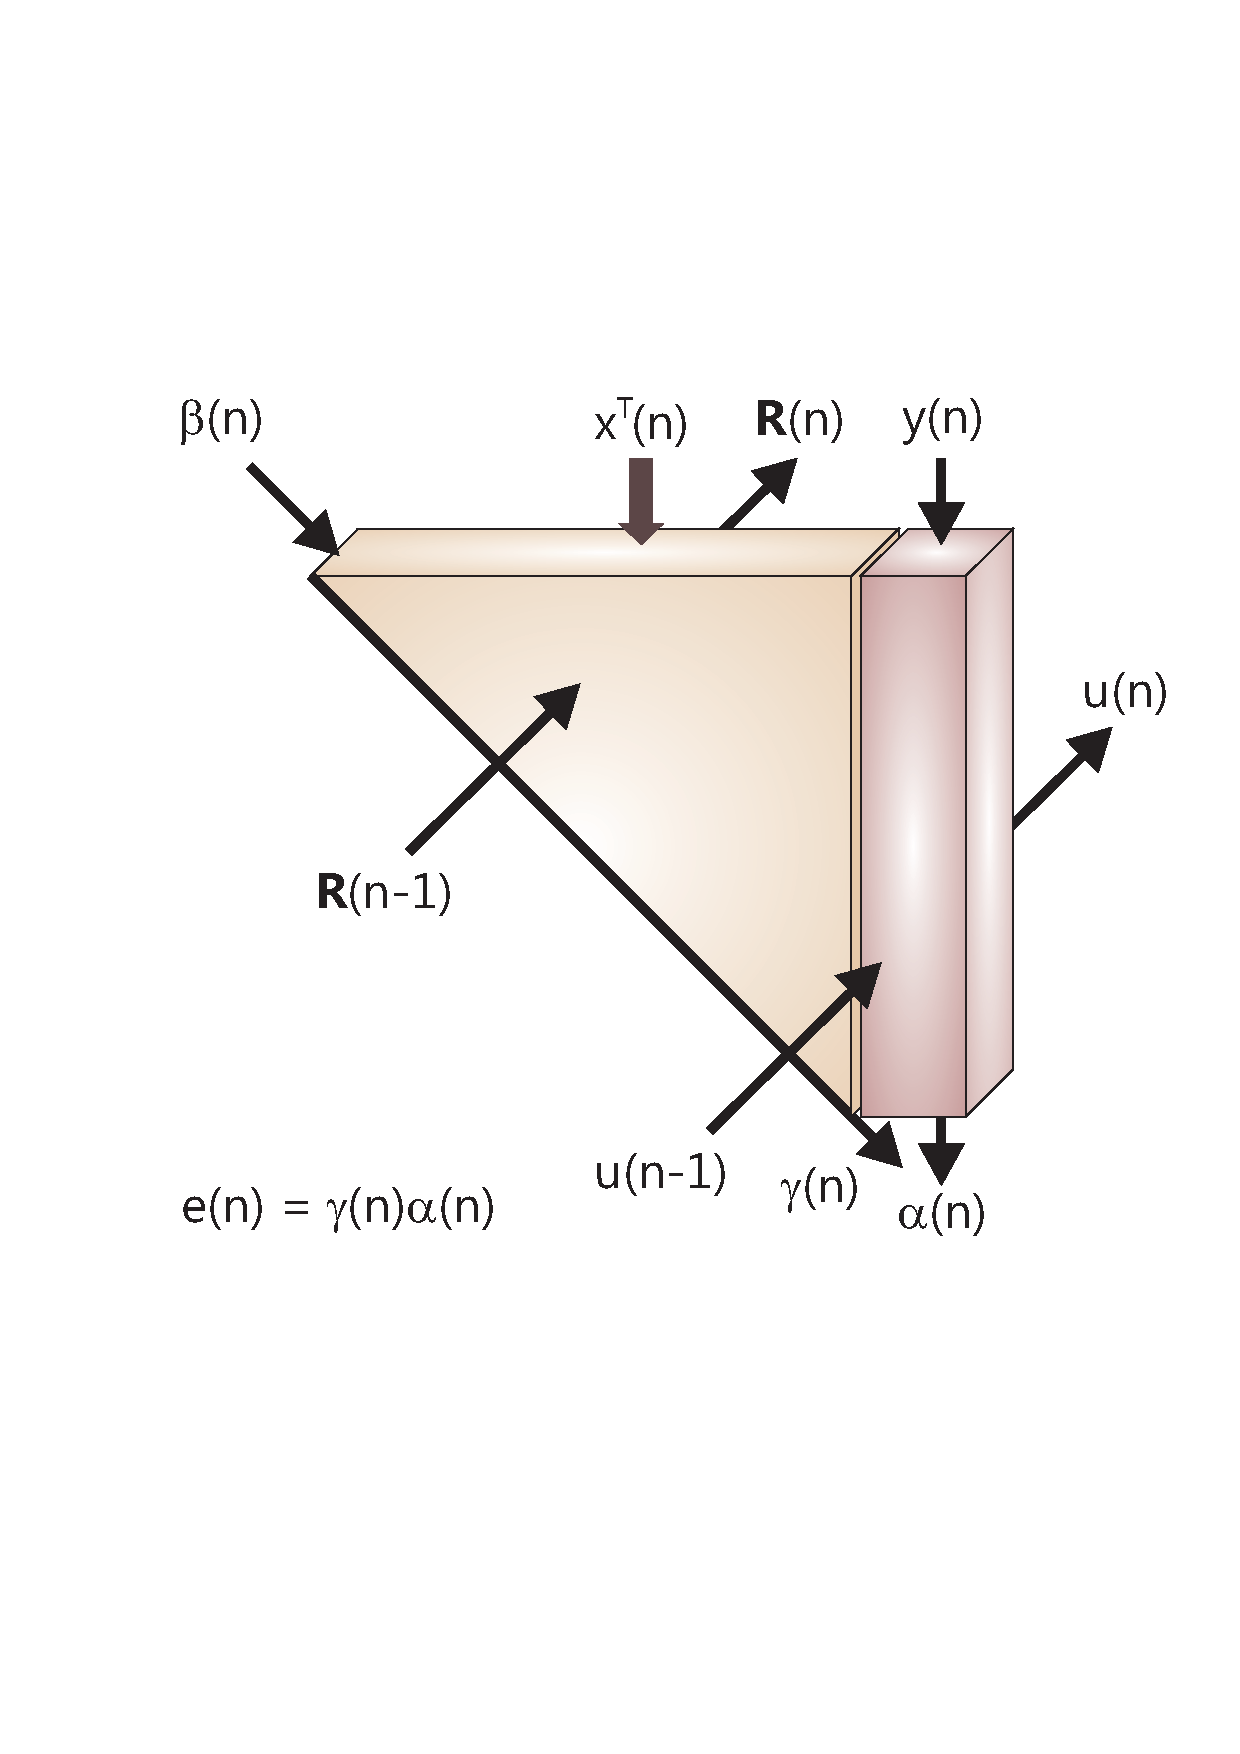
\includegraphics[width=6cm]{./figures/C03-dependence_graph}
        \caption{Gráfico de dependencias en alto nivel para la solución QR-RLS}
        \label{fig:dependence_graph}
\end{figure}

La matriz $X(n)$ es pre-multiplicada por matrices de rotación, un elemento a la vez. Los parámetros son calculados de forma que los elementos por debajo de la diagonal en la primera columna sean convertidos a cero. Luego se sigue con los elementos de la siguiente columna, hasta que la matriz triangular superior equivalente es conformada.

Givens logra esta operación a través de una secuencia de rotaciones, que se pueden explicar utilizando el siguiente ejemplo para una matriz de $2\times3$:

\[
M=
	\left[
		\begin{array}{ccc}
			a_{11} & a_{12} & a_{13} \\
			a_{21} & a_{22} & a_{23}
		\end{array}
	\right]
\]

La matriz es transformada en una matriz pseudo-triangular al eliminar el elemento $a_{21}$. Esto se logra a través de la multiplicación de la siguiente matriz de rotación con la matriz $M$:

\[
G=
	\left[
		\begin{array}{cc}
			 \cos\alpha & -\sin\alpha\\
			 \sin\alpha &  \cos\alpha
		\end{array}
	\right]
\]

Luego:

\[
	\left[
		\begin{array}{cc}
			 \cos\alpha & -\sin\alpha\\
			 \sin\alpha & \cos\alpha
		\end{array}
	\right]
	\left[
		\begin{array}{ccc}
			a_{11} & a_{12} & a_{13} \\
			a_{21} & a_{22} & a_{23}
		\end{array}
	\right]
	= 
\]
\[
	\left[
		\begin{array}{ccc}
			 a_{11}\cos\alpha-a_{21}\sin\alpha &
			 a_{12}\cos\alpha-a_{22}\sin\alpha &
			 a_{13}\cos\alpha-a_{23}\sin\alpha \\
			 a_{11}\sin\alpha+a_{21}\cos\alpha &
			 a_{12}\sin\alpha+a_{22}\cos\alpha &
			 a_{13}\sin\alpha+a_{23}\cos\alpha
		\end{array}
	\right]
\]

Para eliminar $a_{21}$ se debe resolver $a_{11}\sin\alpha+a_{21}\cos\alpha = 0$. Luego, por trigonometría, se puede plantear la siguiente solución:

\begin{align}
\cos\alpha &=  a_{11} / \sqrt{a_{11}^2 + a_{21}^2}\\
\sin\alpha &= -a_{21} / \sqrt{a_{11}^2 + a_{21}^2}\\
 a_{11new} &= \sqrt{a_{11}^2 + a_{21}^2}\\
 a_{21new} &= 0
\end{align}

Aplicando la rotación para eliminar $a_{21}$ resulta en la matriz pseudo-triangular:

\[
M=
	\left[
		\begin{array}{ccc}
			a_{11new} & a_{12new} & a_{13new} \\
			    0     & a_{22new} & a_{23new}
		\end{array}
	\right]
\]

Esta función puede implementarse en un arreglo sistólico, como se ve en la figura \ref{fig:rls_givens_rotations}, el cual consiste en dos tipos de celdas, referidas como \textit{boundary cell} (BC - representada con un círculo) e \textit{internal cell} (IC - representada con un cuadrado).

\begin{figure}[h!]
        \centering
        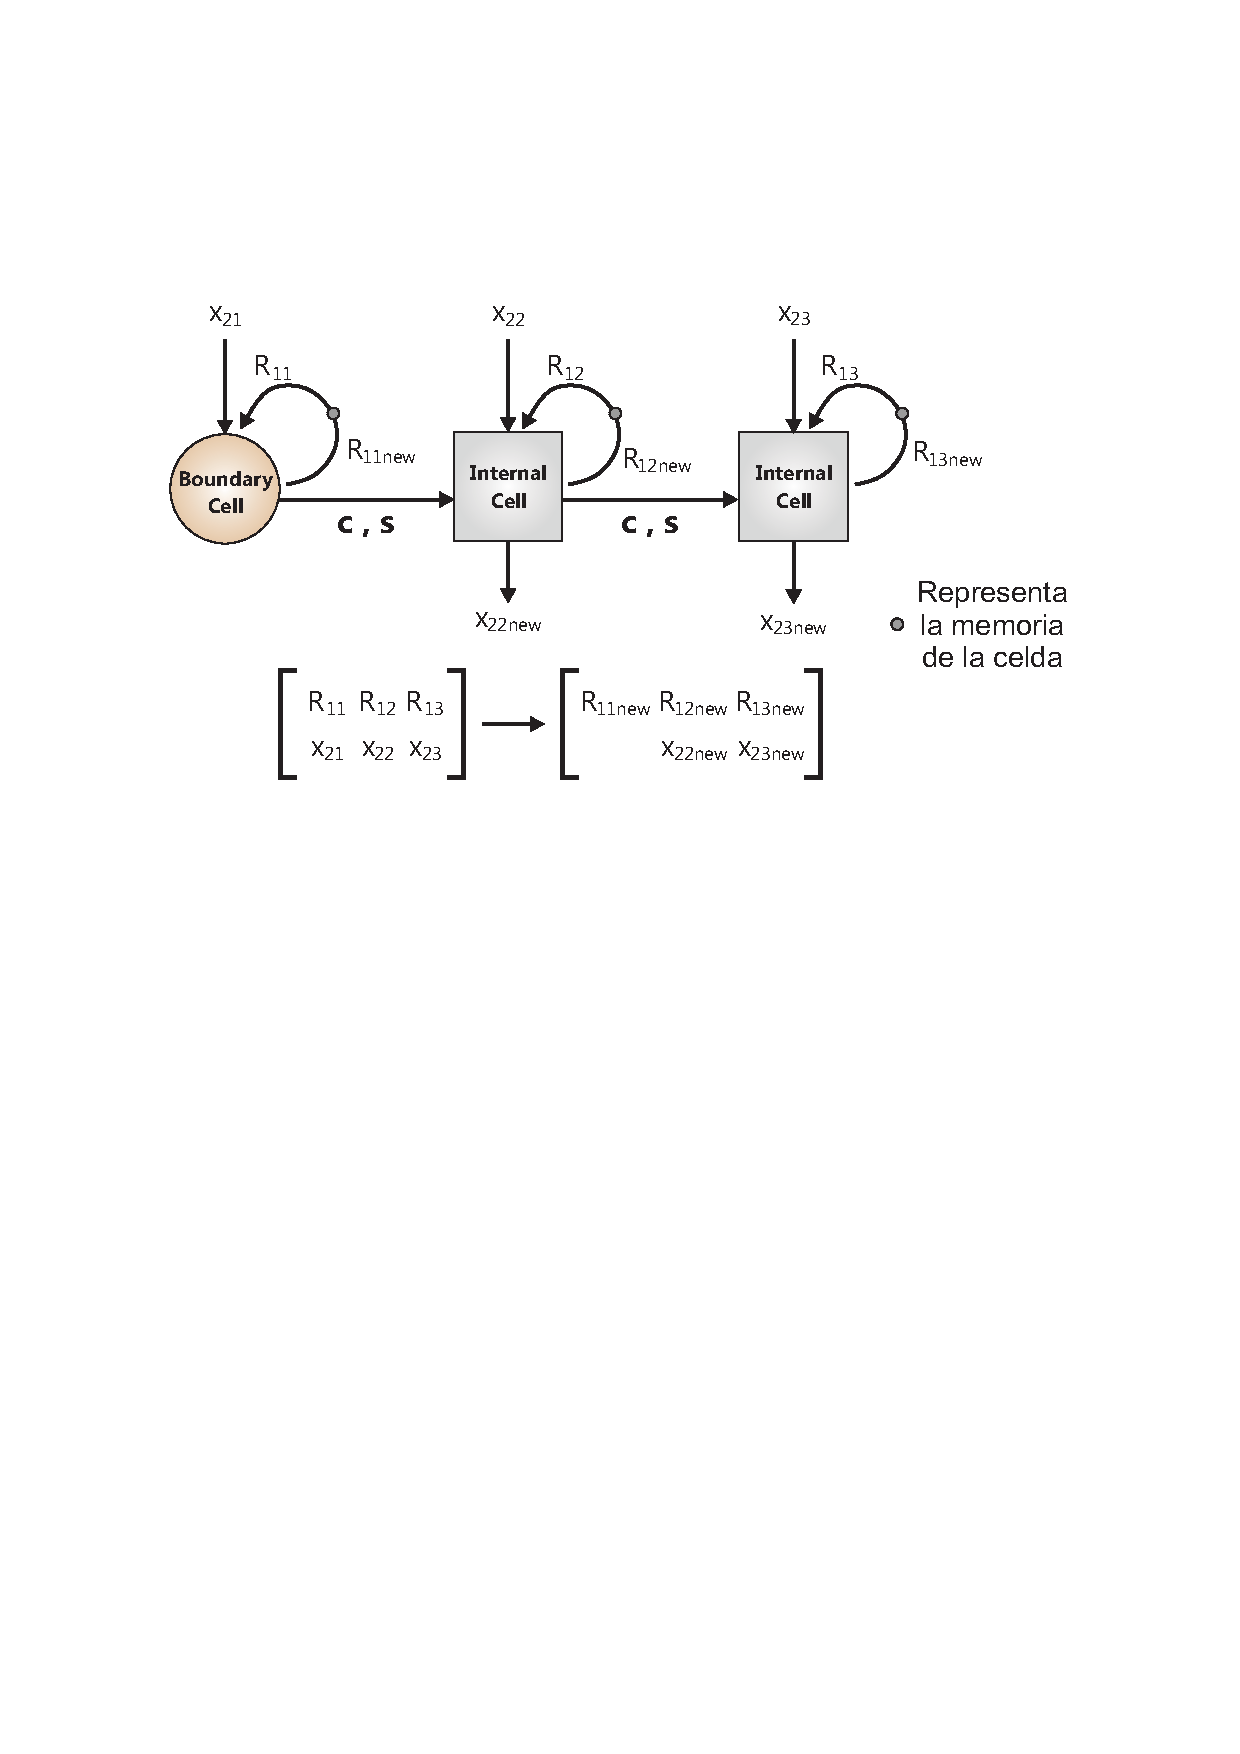
\includegraphics[width=10cm]{./figures/C03-rls_givens_rotations}
        \caption{Transformación por Rotaciones de Givens}
        \label{fig:rls_givens_rotations}
\end{figure}

Los elementos en los cuales se aplican las rotaciones son $x$ y $R$, donde $x$ es el valor de entrada en la celda, y $R$ es el valor retenido en la memoria para esa celda. Los parámetros de rotación, $\cos\alpha$ y $\sin\alpha$, son calculados en una \textit{boundary cell}, de forma tal que el valor de $x$ que ingresa a una \textit{boundary cell} sea convertido a 0, y el valor de R de dicha celda sea actualizado acorde a la rotación y almacenado para la próxima iteración.

Los parámetros de rotación son enviados sin modificar a lo largo de toda una fila a cada una de las \textit{internal cells} para continuar con la rotación. El gráfico de dependencia de la figura \ref{fig:rls_givens_rotations} representa la eliminación de $x_{21}$, relacionado con el elemento de la matriz $a_{21}$ del ejemplo anterior. Los valores de $R$ y $x$ son considerados una coordenada polar $(R, x)$.

Eliminar la entrada $x$ en una \textit{boundary cell}, se logra a través de rotar el vector un ángulo $\alpha$ tal que:

\[
R_{new} = R \cos\alpha - x \sin\alpha = \frac{R^2 + x^2}{\sqrt{R^2 + x^2}} = \sqrt{R^2 + x^2}
\]

donde

\[
\cos\alpha = \frac{R}{R_{new}} = c
\hspace{3cm}
\sin\alpha = \frac{-x}{R_{new}} = s
\]

Los mismos parámetros de rotación utilizados en BC son aplicados en las ICs:

\[
R_{new} = cR - sX \hspace{3 cm}
x_{new} = cx + sR
\]

Al concatenar rotaciones de Givens sucesivas, la factorización QR puede ser implementada para una matriz $N \times N$. El diagrama de la figura \ref{fig:givens_for_3x3} muestra un ejemplo para una matriz de $3 \times 3$. Se trata de un esquema \textit{pipeline} en el cual los valores de R son realimentados a sus propias celdas para la próxima iteración.

\begin{figure}[h!]
        \centering
        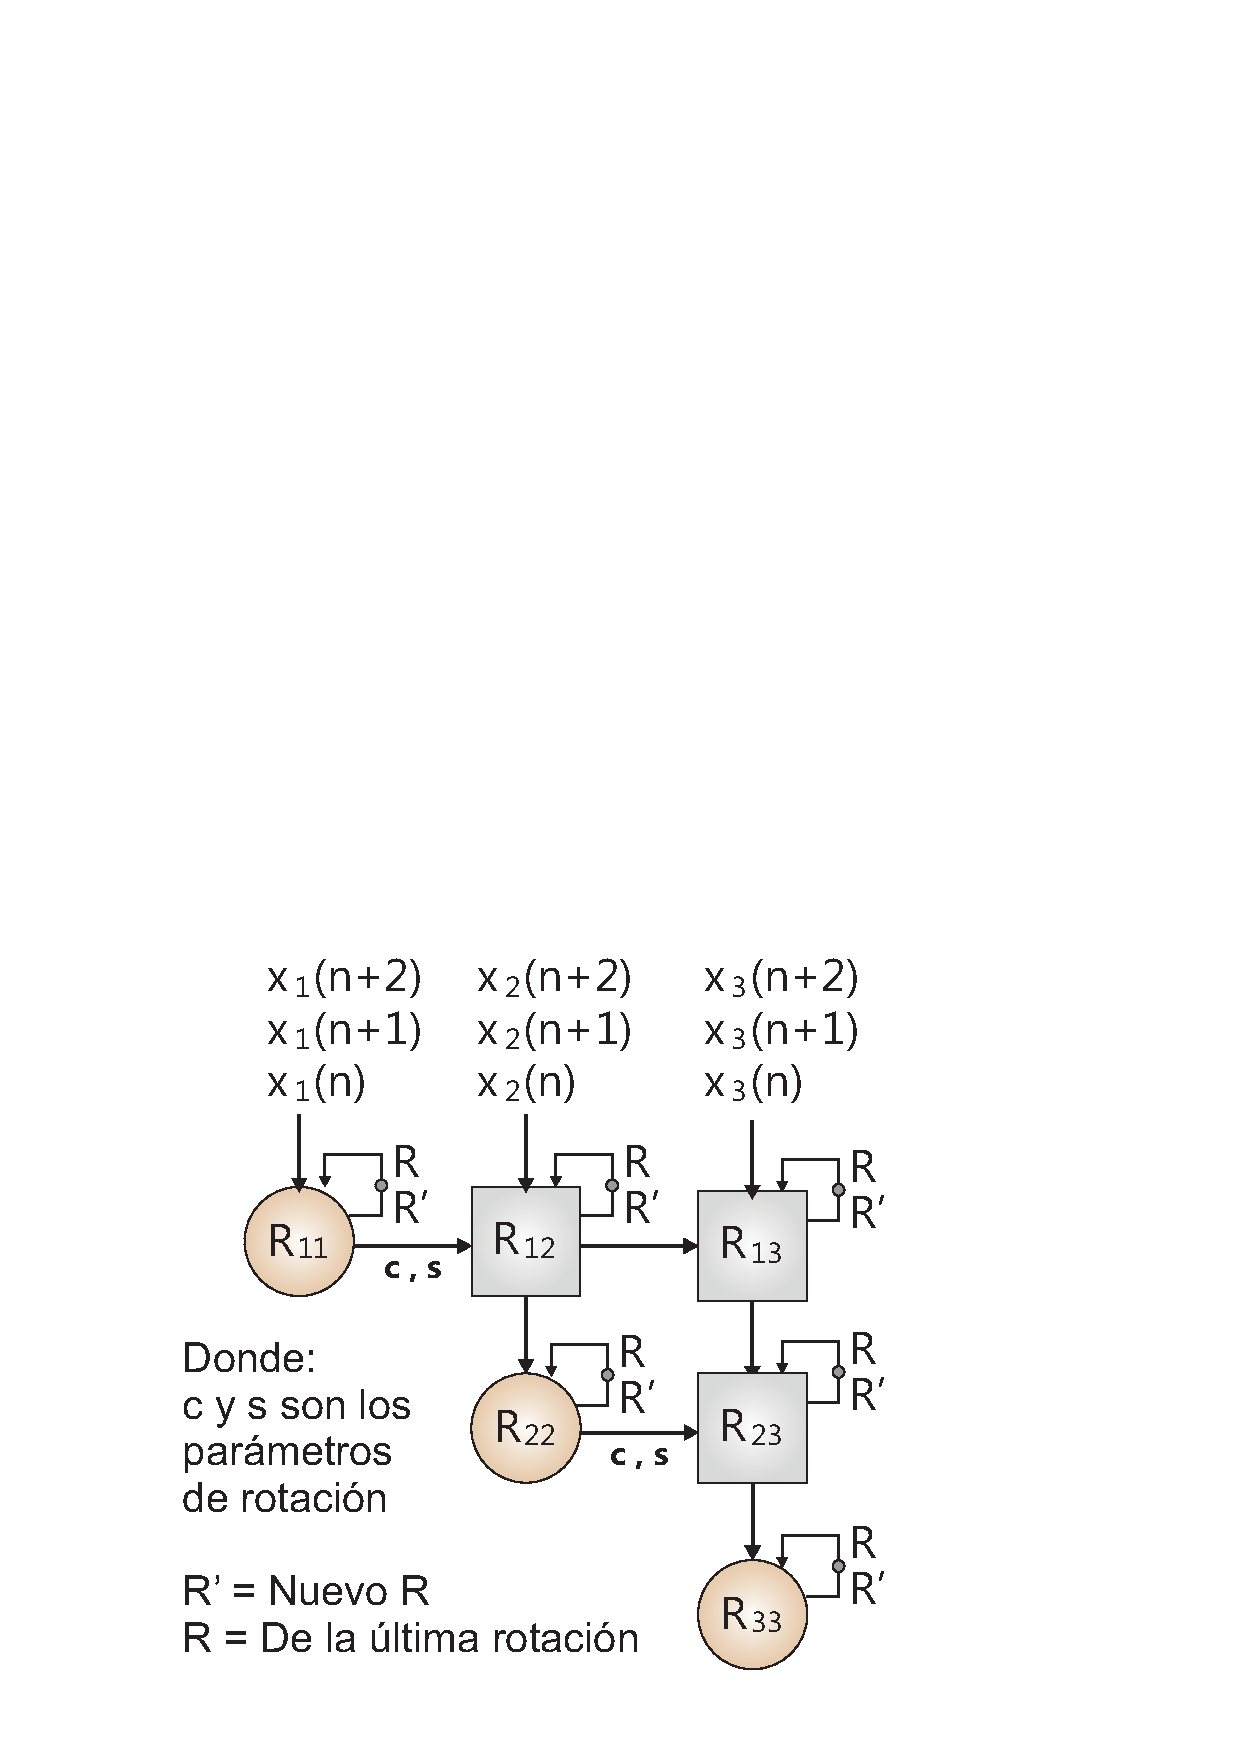
\includegraphics[width=5cm]{./figures/C03-givens_for_3x3}
        \caption{Descomposición QR aplicada a una matriz de 3x3}
        \label{fig:givens_for_3x3}
\end{figure}

A continuación se explorará en un nivel más detallado el proceso de desarrollar una arquitectura en hardware desde el algoritmo RLS y sus ecuaciones resuelto por descomposición QR utilizando rotaciones de Givens.

\section{Del algoritmo a una arquitectura sintetizable}

Con el objetivo de lograr la implementación, es necesario transformar las ecuaciones presentadas en una arquitectura sintetizable. En este proceso, es un aspecto clave el lograr una implementación de un circuito de alta \textit{performance}, para asegurar una traducción eficiente del algoritmo a hardware en silicio. Esto normalmente conlleva el hecho de desarrollar una arquitectura en la cual operaciones independientes se desarrollen en paralelo para aumentar el rendimiento.

En la figura \ref{fig:development_process} se presenta el proceso de transformar las ecuaciones a un procesador en hardware.

\begin{figure}[h!]
        \centering
        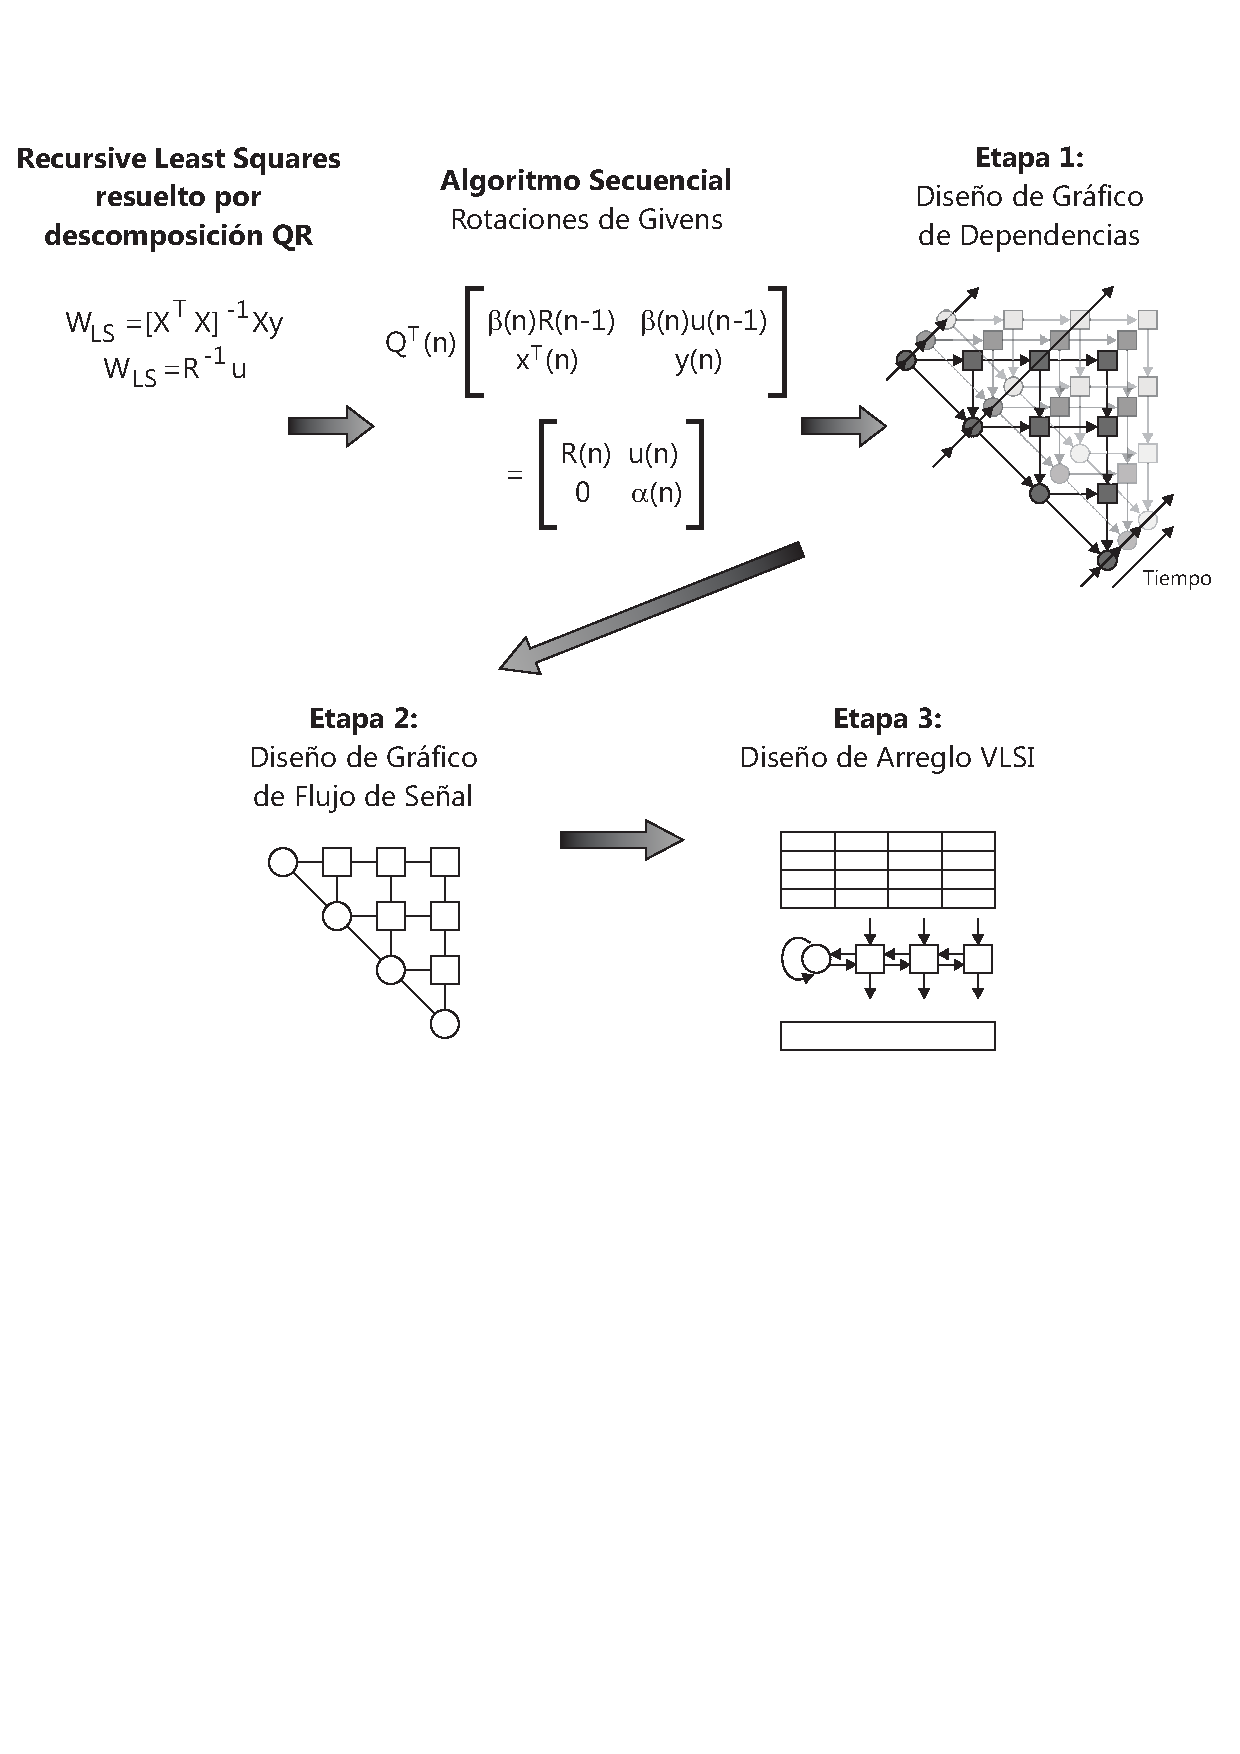
\includegraphics[width=14cm]{./figures/C03-development_process}
        \caption{Proceso de desarrollo del circuito digital}
        \label{fig:development_process}
\end{figure}

El punto de inicio en la figura es la resolución del algoritmo RLS a través de la descomposición QR. La siguiente etapa muestra dicha resolución a través del uso de un algoritmo secuencial. Esto es, por cada iteración del algoritmo, un nuevo conjunto de valores ingresa a las ecuaciones y evoluciona a una nueva solución.

La operación QR puede representarse como un arreglo triangular de operaciones. La matriz de información es la entrada en la parte superior del triángulo, y en cada fila son eliminados los términos para resultar en una matriz triangular superior.

El gráfico de dependencias en la figura \ref{fig:development_process} expone este proceso de triangularización. Los arreglos triangulares en cascada representan \textbf{cada iteración en el tiempo}. Las flechas muestran la dependencia a través del tiempo. Desde el diagrama de dependencias, se desarrolla posteriormente un diagrama de flujo de señal adecuado, y con el mismo se deriva una arquitectura sintetizable.

\subsection{Gráfico de dependencias}

En este diagrama se pueden detectar las dependencias entre los datos, permitiendo identificar el máximo nivel de concurrencia posible al desensamblar el algoritmo en nodos y flechas. Los nodos representan los cálculos y la dirección de las flechas la dependencia de las operaciones. En la figura \ref{fig:dependence_vs_signal} se muestra un ejemplo de $3 \times 3$. Cada esquema en perspectiva representa una iteración en el tiempo (para $n$, $n+1$ y $n+2$). Las flechas demuestran que, por ejemplo, para hacer el cálculo de $a_{12}$, se requiere la salida del procesamiento realizado en $a_{11}$, o que para hacer el cálculo de $a_{22}$, se requiere la salida de los procesamientos realizados en $a_{11}$ y $a_{12}$.

\begin{figure}[h!]
        \centering
        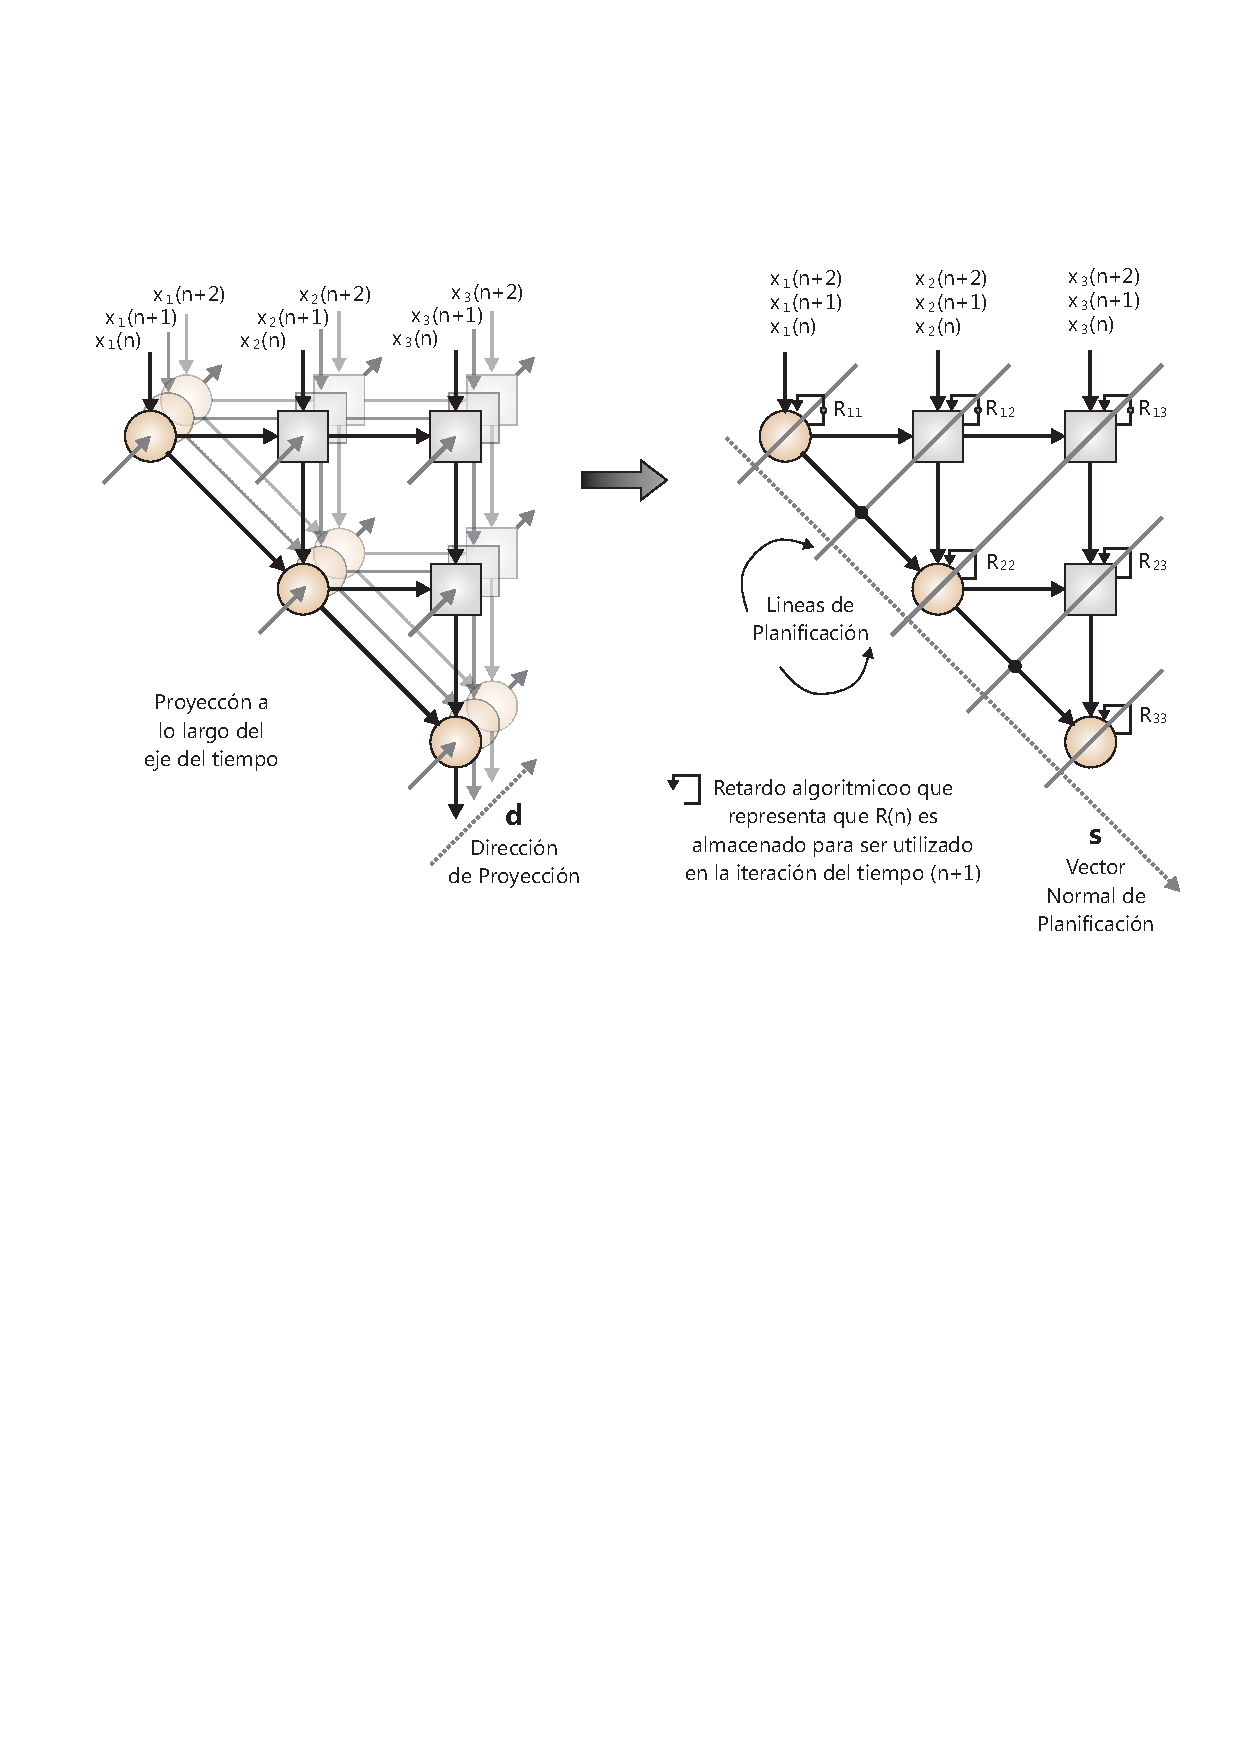
\includegraphics[width=12cm]{./figures/C03-dependence_vs_signal}
        \caption{Gráfico de Dependencias y Gráfico de Flujo de Señal}
        \label{fig:dependence_vs_signal}
\end{figure}

\subsection{Gráfico de flujo de señal}

En la figura \ref{fig:dependence_vs_signal}, se puede observar la transición del gráfico de dependencias al gráfico de flujo de señal. Este es el gráfico de mayor importancia para derivar a una arquitectura, dado que representa el sentido en el cual deben transmitirse las señales, y el orden en el cual se deben realizar las operaciones. Los nodos del gráfico de dependencias son asignados a procesadores, y sus operaciones son planificadas entre los mismos.

Una de las formas más sencillas para lograr esta transición es \textbf{la proyección lineal de todos los nodos idénticos} a lo largo de una linea recta en un único procesador. Esto es representado por el vector de proyección $\mathbf{d}$. La planificación lineal es utilizada para determinar el orden en el cual las operaciones son realizadas en estos procesadores. Las \textbf{líneas de planificación} en la figura \ref{fig:dependence_vs_signal} \textbf{indican las operaciones que se pueden realizar en paralelo} en cada ciclo de reloj. Matemáticamente están representadas por un \textbf{vector de planificación} $\mathbf{s}$ normal a las líneas de planificación, el cual apunta en la dirección de la dependencia de las operaciones (muestra el orden en el cual cada línea de operaciones es realizada).

Existen dos reglas que gobiernan la proyección y la planificación:

\begin{itemize}
	\item[•] Todos los arcos de dependencia fluyen en la misma dirección a lo largo de las líneas de planificación.
	\item[•] Las líneas de planificación no son paralelas con el vector de proyección $\mathbf{d}$.
\end{itemize}

En el ejemplo QR, cada arreglo triangular de celdas en el diagrama de dependencias representa una actualización QR. Al estar en cascada, el diagrama representa una \textbf{secuencia de actualizaciones QR}. Al proyectar a lo largo del eje del tiempo, todas las actualizaciones QR pueden ser asignadas a un diagrama de flujo de señal triangular, como se observa en la imagen.

Los valores $R$ son transmitidos a lo largo del tiempo de una actualización QR a la otra, representados por la cascada de arreglos triangulares. Esta transición se observa mejor en el diagrama de flujo de señal en la realimentación de los valores $R$ en la celda a partir de un \textit{delay} algorítmico utilizado para retener los valores hasta la próxima iteración. Esto es referido como un lazo recursivo.

La simplicidad del diagrama de flujo de señal es que asume que todas las operaciones en los nodos ocupan un único ciclo, así como los \textit{delays} algorítmicos, representados por pequeños círculos oscuros. Estos \textit{delays} algorítmicos particionan las iteraciones del algoritmo y son una parte necesaria del mismo. El resultado del diagrama de flujo de señal es una representación más concisa del algoritmo con respecto al diagrama de dependencias.

El camino a seguir, una vez definido el diagrama de flujo de señal, es derivar una arquitectura eficiente e implementar en hardware el algoritmo.

\newpage

\section{Implementación sistólica de las rotaciones de givens}

A partir del gráfico de flujo de señal, se debe profundizar el mismo a un nivel de detalle que defina la forma en la cual se implementarán los procesadores, la cantidad de los mismos que van a ser utilizados, la forma en la cual se almacenarán los datos, y cómo se realizará el control de los mismos. Existen diferentes mapeos desarrollados para derivar del arreglo triangular una arquitectura sintetizable. Veremos a continuación algunos de ellos.

\subsection{Mapeo de Gentleman y Kung}
\label{sec:mapeo_de_gentleman_y_kung}

El modo más directo de transformar el algoritmo en una arquitectura sintetizable consiste en la implementación de un arreglo sistólico en el cual cada \textit{boundary cell} e \textit{internal cell} sea calculada por un procesador independiente. Dicho esquema se presenta en la figura \ref{fig:direct_mapping}. 

\begin{figure}[h!]
        \centering
		\begin{minipage}[b]{0.4\textwidth}
			\footnotesize
			\[ [x_1(n) x_2(n) x_3(n)] = \underline{x}^T(n) \]
			\[ \left[
					\begin{array}{ccc}
						R_{11}(n-1) & R_{12}(n-1) & R_{13}(n-1) \\
							        & R_{22}(n-1) & R_{23}(n-1) \\
							        & 			  & R_{33}(n-1)
					\end{array}
				\right] = R(n-1) \]
			\[ \left[
					\begin{array}{c}
						u_{14}(n-1) \\
						u_{24}(n-1) \\
						u_{34}(n-1)
					\end{array}
				\right] = u(n-1) \]\vspace{1 cm}\\
			\normalsize
		\end{minipage}%
		\begin{minipage}[b]{0.6\textwidth}
        	\centering
        	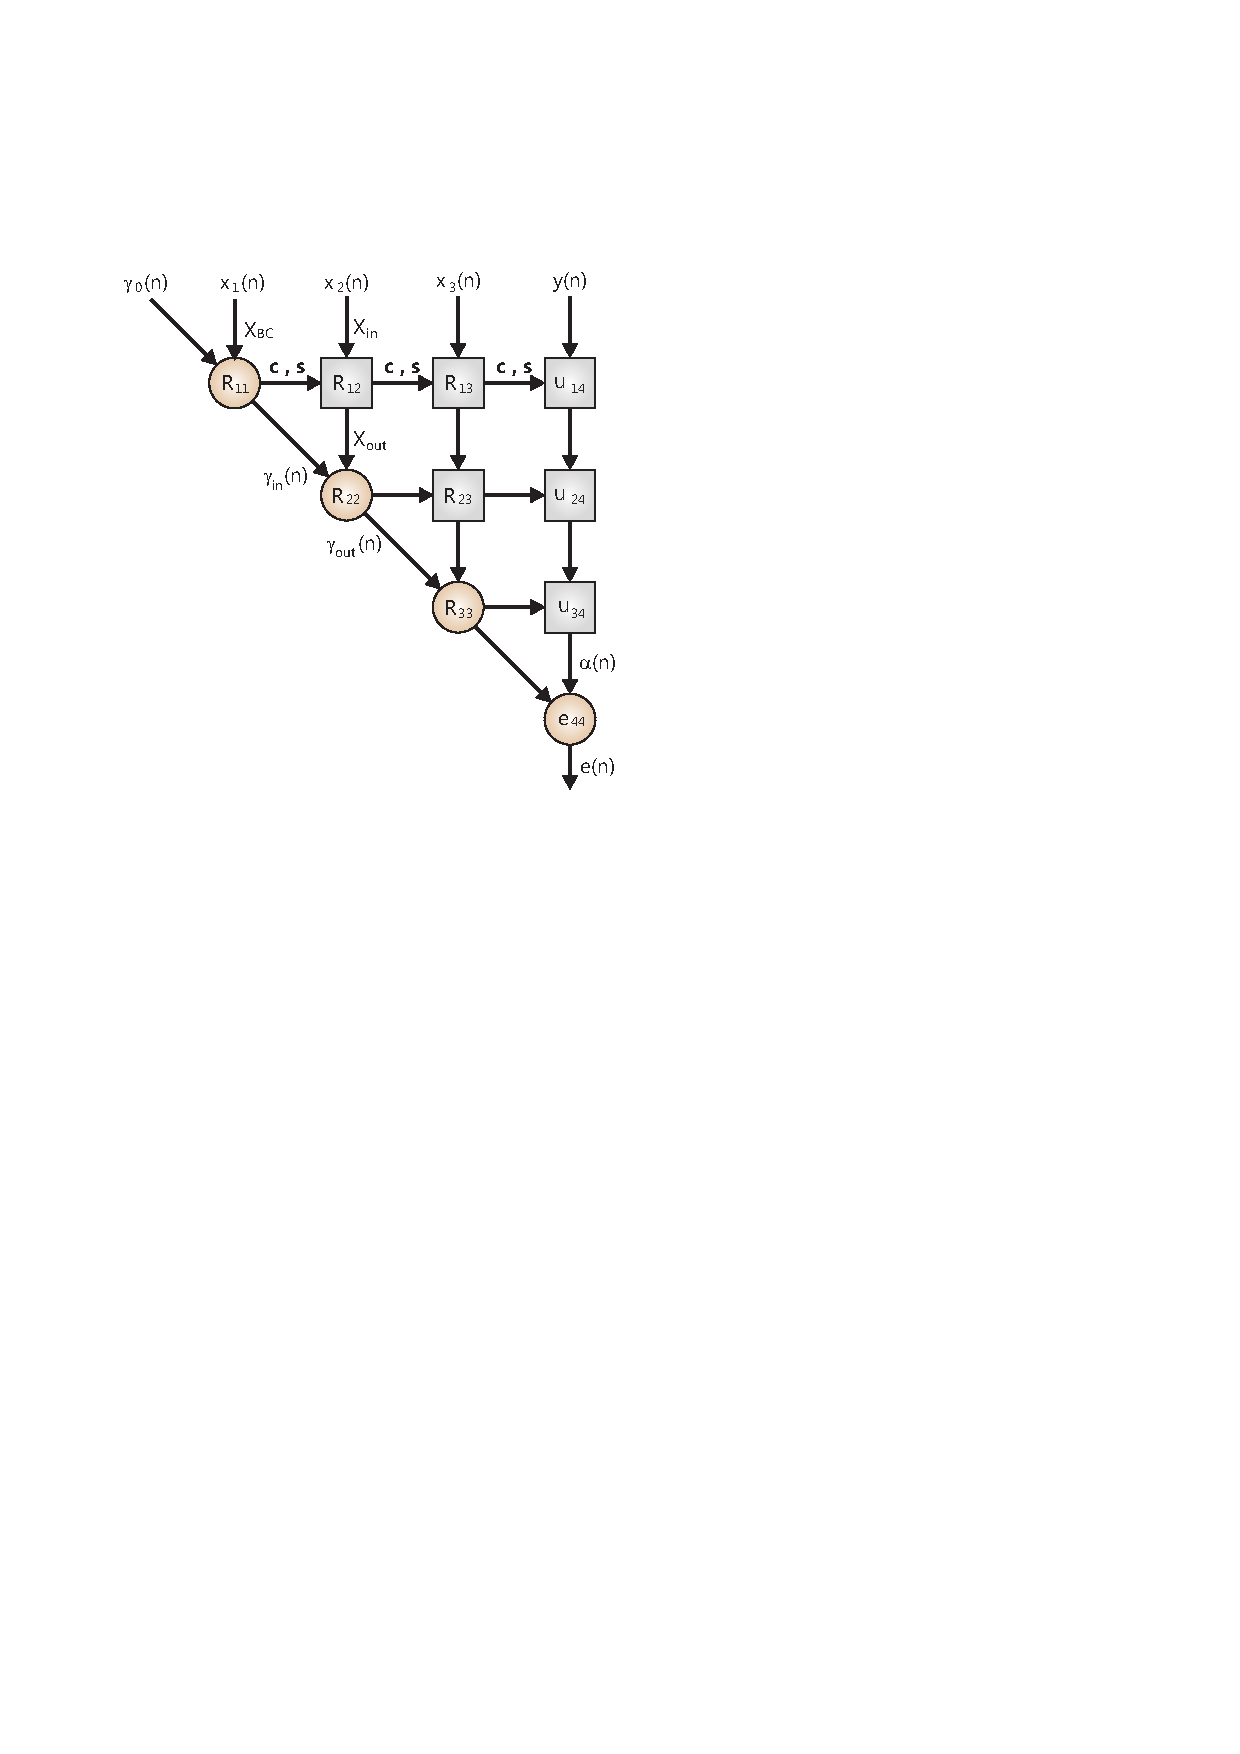
\includegraphics[width=6cm]{./figures/C03-direct_mapping}
        \end{minipage}%
        \caption{Esquema de mapeo directo}
        \label{fig:direct_mapping}
\end{figure}

Esta arquitectura fue desarrollada por Gentleman y Kung y modificada por McWhirter. En la misma, el vector de información $\mathbf{x}^T(n)$ ingresa al sistema desde la parte superior del arreglo y es progresivamente eliminado al computar la rotación en cada fila de la matriz en proceso. Los parámetros $c$ y $s$ son calculados en una BC de forma que eliminen la entrada $x_{i,i}(n)$. Estos parámetros son posteriormente enviados a las ICs de la misma fila para actualizar las componentes según el resultado de la rotación aplicada. Los valores de salida de las ICs $x_{i+1,j}(n)$ se convierten en los valores de entrada para la próxima fila. Al mismo tiempo, una nueva entrada ingresa en la parte superior del arreglo y el proceso se repite. En el proceso, los valores de $R(n)$ y $u(n)$ son actualizados para registrar la rotación y luego almacenados en el arreglo para ser utilizados en el próximo ciclo.

Para el algoritmo RLS, la implementación del factor de olvido $\lambda$ y el producto de cosenos $\gamma$ debe ser incluido en las ecuaciones. Por lo tanto, las operaciones de BC e IC son modificadas acordemente. Una notación es asignada a las variables en el arreglo. Cada término $R$ y $u$ posee un sub-índice denotado por (i,j), que representa la ubicación de los elementos en la matriz $R$ y el vector $u$. Una notación similar es asignada a las entradas $X$ y a las variables de salida. Las descripciones de las celdas para las BCs e ICs son presentadas en las figuras \ref{fig:direct_mapping_2} y \ref{fig:direct_mapping_3} respectivamente.

\begin{figure}[h!]
        \centering
        \begin{minipage}[b]{0.4\textwidth}
        	\centering
            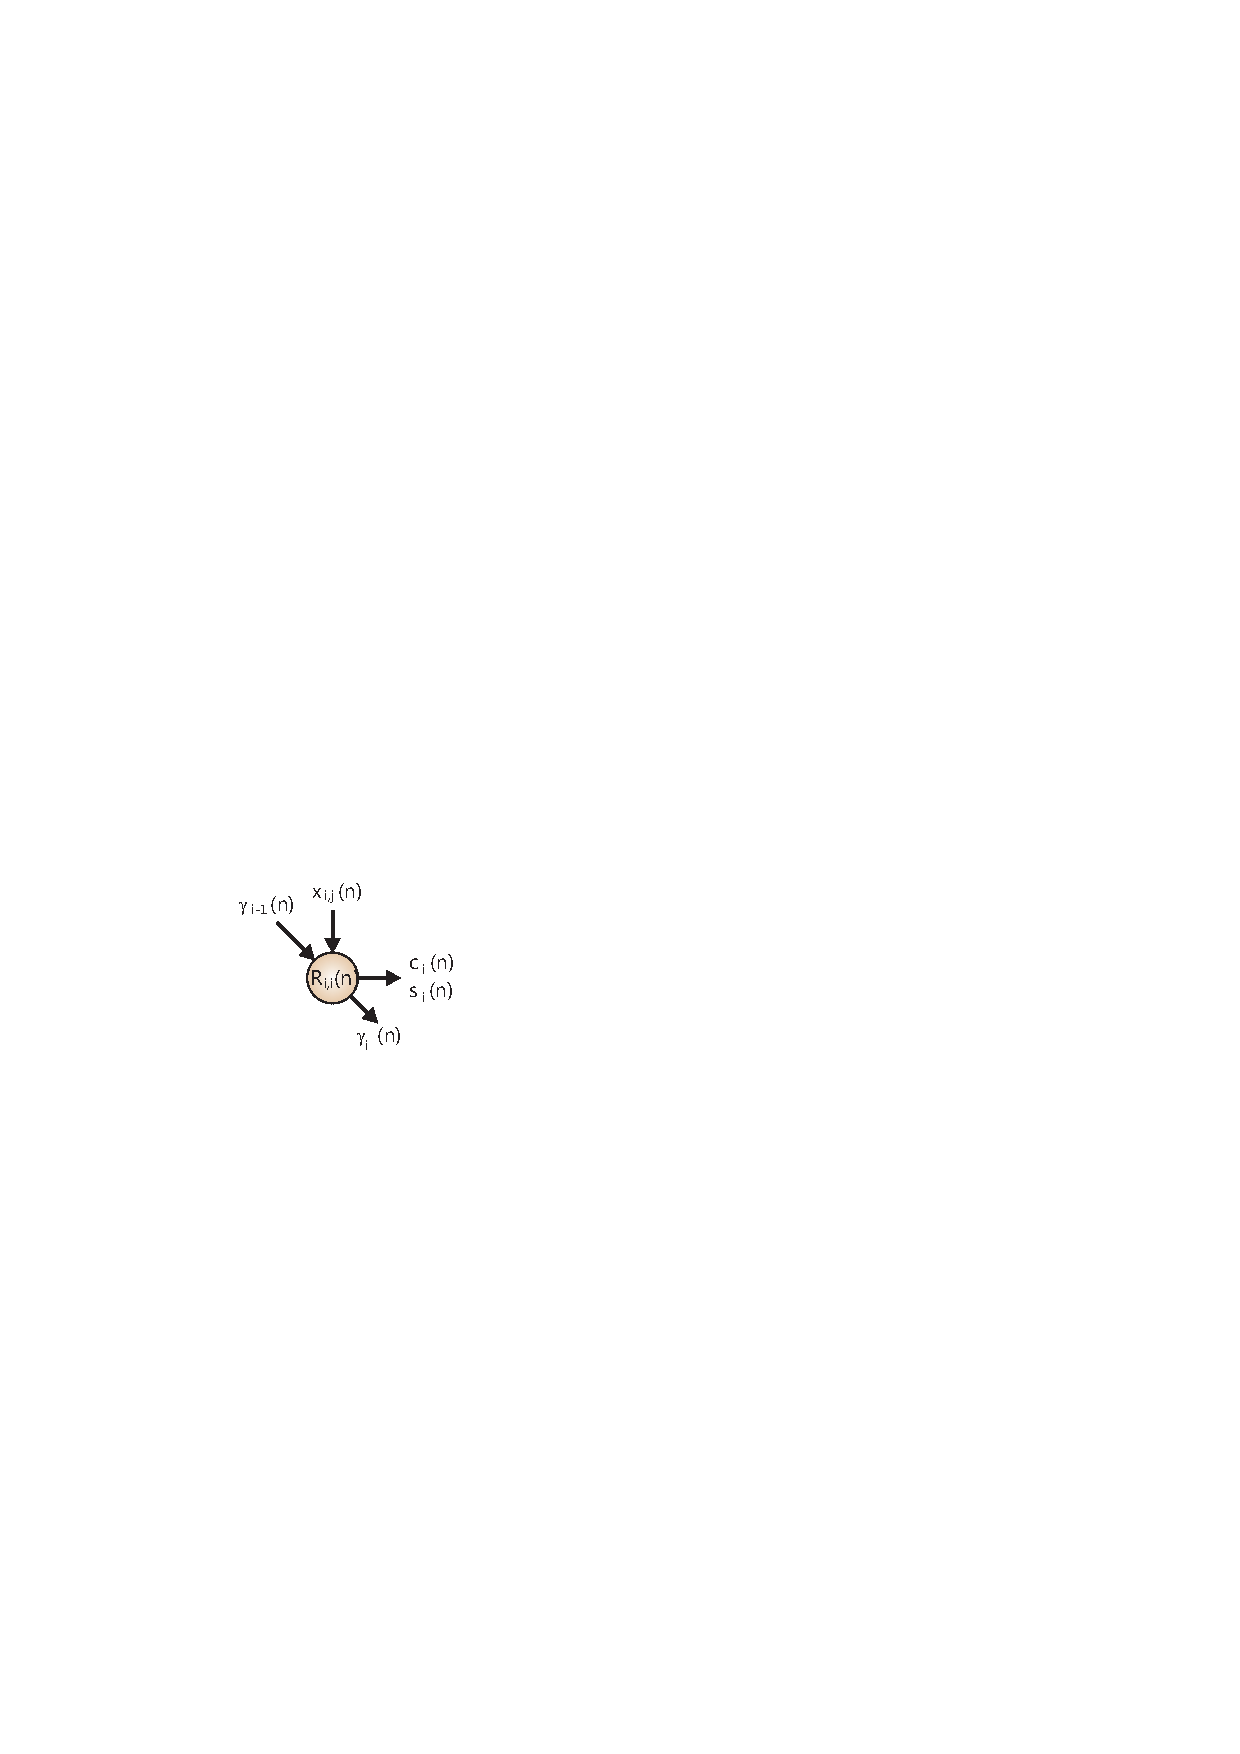
\includegraphics[width=3 cm]{./figures/C03-bc}
            \caption{Boundary Cell}
            \label{fig:direct_mapping_2}
        \end{minipage}%
		\begin{minipage}[b]{0.6\textwidth}
			\small
			\begin{equation}
			\label{eq:boundary_cell_1}
			R_{i,i}(n) = \sqrt{\beta^2 R_{i,i}^2(n-1) + x^2_{i,i}(n)}
			\end{equation}
			\begin{equation}
			\label{eq:boundary_cell_2}
			c_i(n) = \beta \frac{R_{i,i}(n-1)}{R_{i,i}(n)}
			\end{equation}
			\begin{equation}
			\label{eq:boundary_cell_3}
			s_i(n) = \frac{x_{i,i}(n-1)}{R_{i,i}(n)}
			\end{equation}
			\[ \gamma_i(n) = c_i(n) \gamma_{i-1}(n-1) \]
			\normalsize
		\end{minipage}%
\end{figure}

\begin{figure}[h!]
        \centering
        \begin{minipage}[b]{0.4\textwidth}
        	\centering
            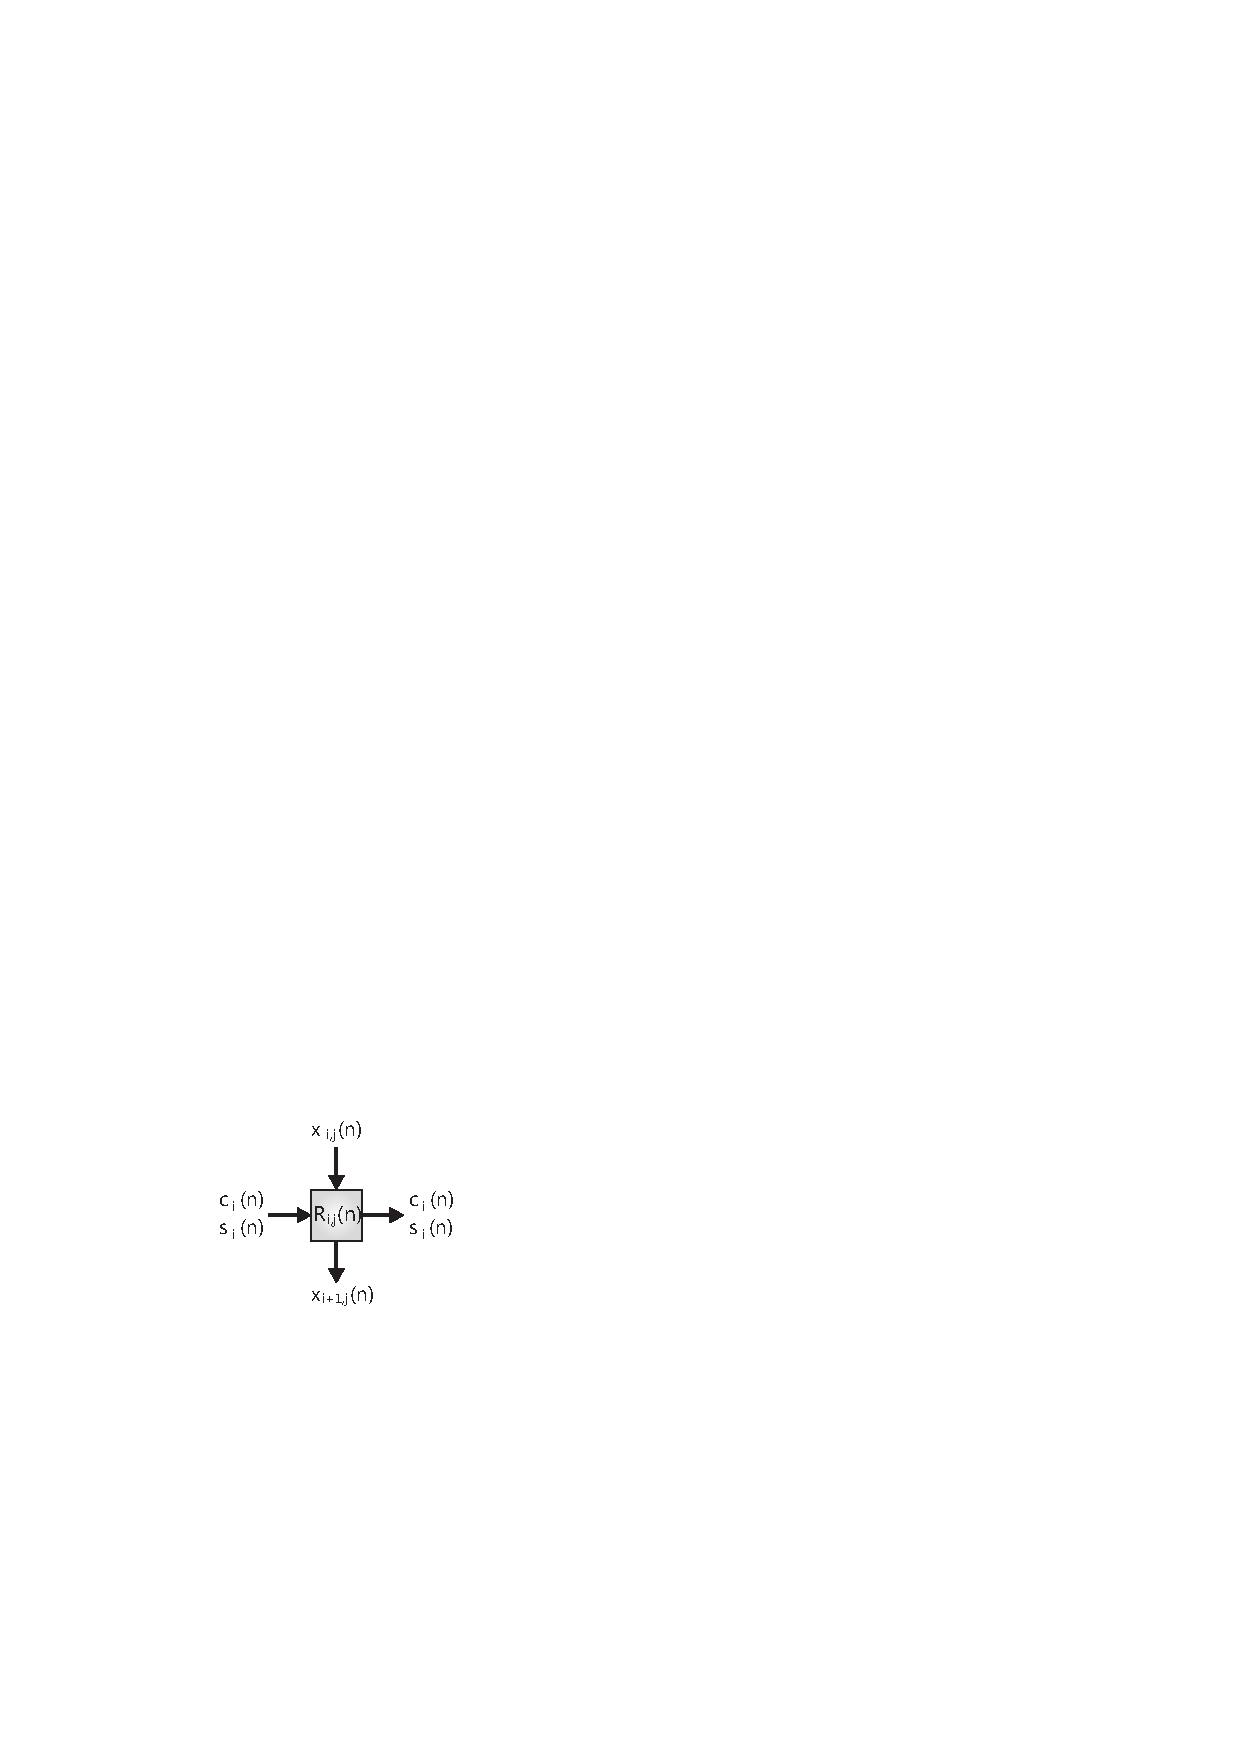
\includegraphics[width=3 cm]{./figures/C03-ic}
            \caption{Internal Cell}
            \label{fig:direct_mapping_3}
        \end{minipage}%
		\begin{minipage}[b]{0.6\textwidth}
			\small
			\begin{equation}
			\label{eq:internal_cell_1}
			x_{i+1,j}(n) = c_i(n) x_{i,j}(n) - s_i(n) \beta R_{i,j}(n-1)
			\end{equation}
			\begin{equation}
			\label{eq:internal_cell_2}
			R_{i,j}(n) = c_i(n) \beta R_{i,j}(n-1) + s_i(n) x_{i,j}(n)
			\end{equation} \\
			\normalsize
		\end{minipage}%
\end{figure}

Se puede destacar que, si bien la implementación de este mapeo es simple y es posible lograr que las celdas operen en un esquema \textit{pipeline}, la implementación requiere una gran cantidad de procesadores (en el ejemplo se tienen 10 para una matriz de $4 \times 4$) por lo cual ocupará un alto porcentaje de recursos del FPGA comparada con otras.

\subsection{Mapeo de proyección horizontal}

En la figura \ref{fig:horizontal_mapping} se puede observar un ejemplo de un mapeo de celdas QR en una arquitectura lineal proyectando de izquierda a derecha en N procesadores. Existen dos conflictos con dicho mapeo.

\begin{figure}[h!]
        \centering
        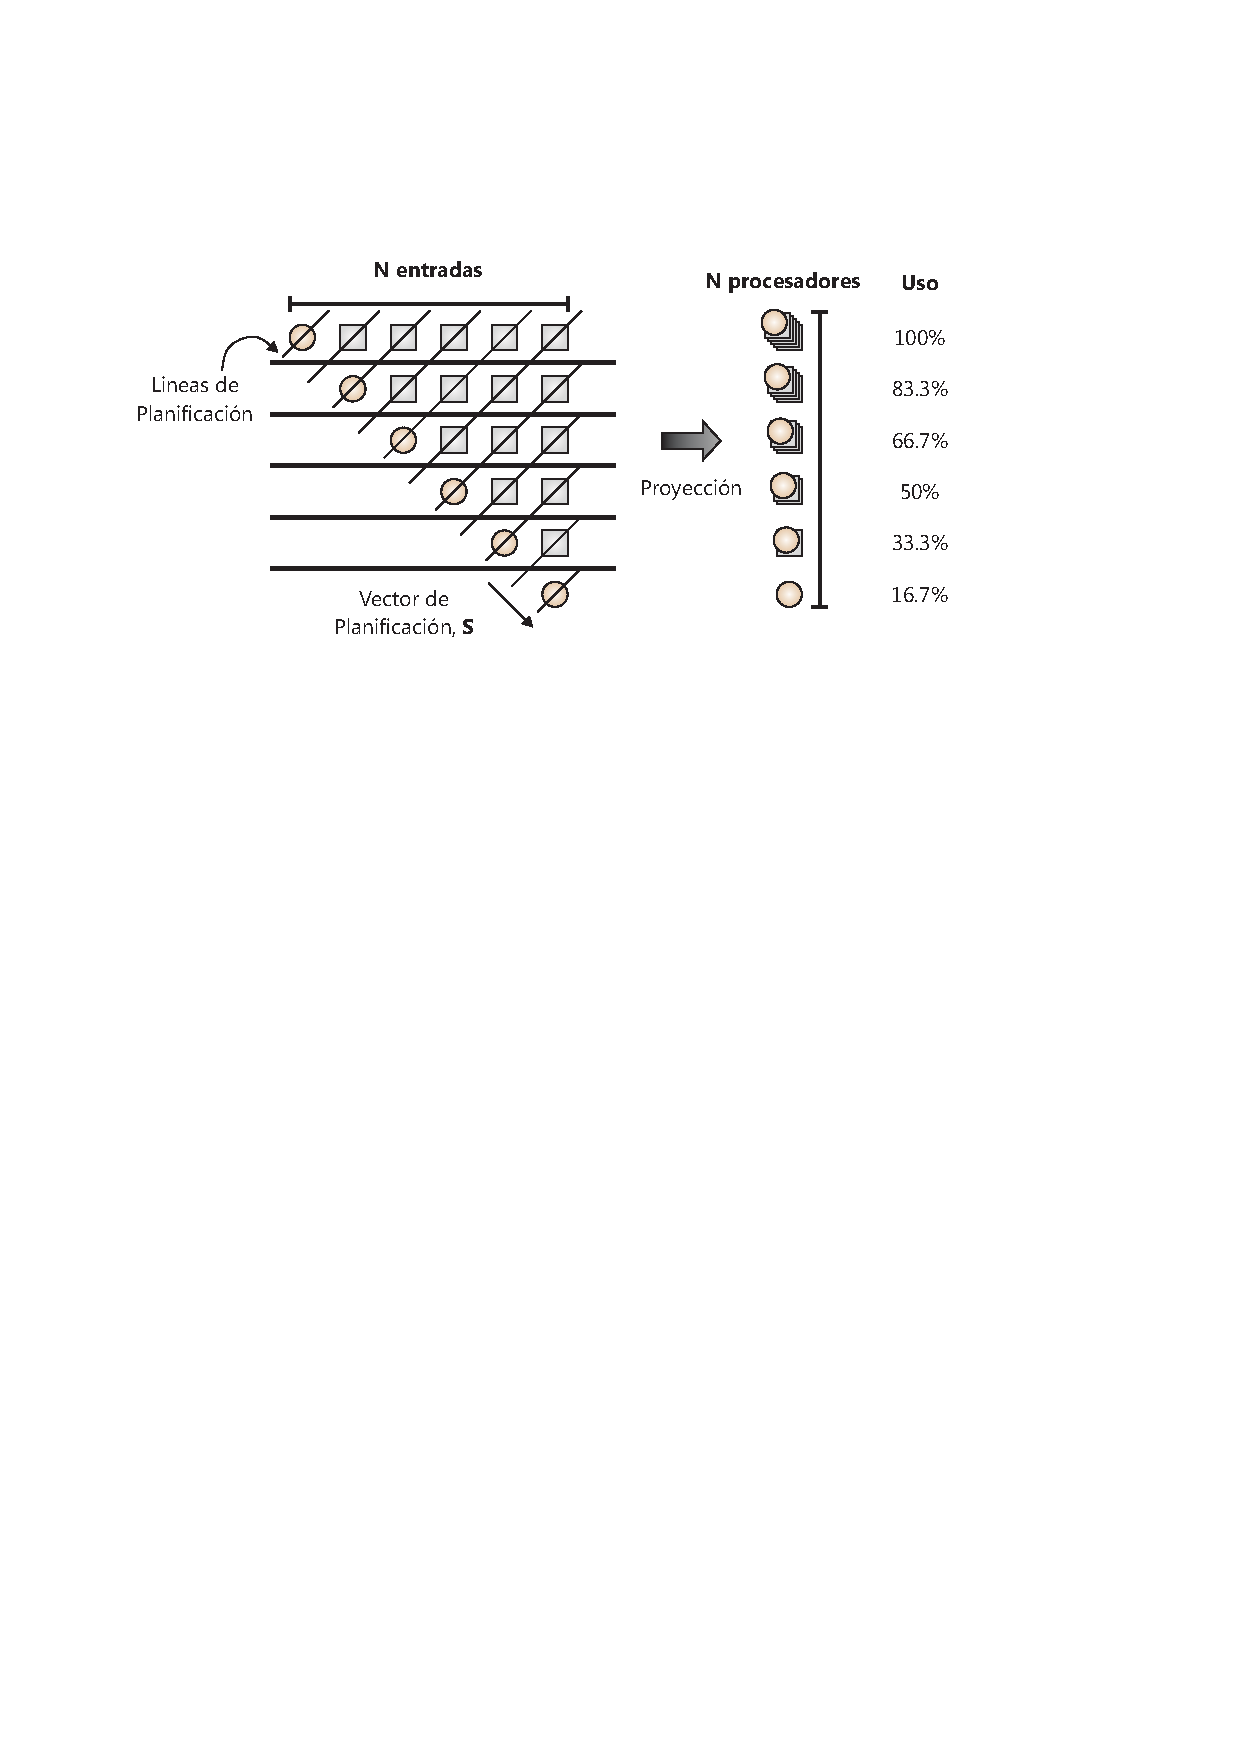
\includegraphics[width=13cm]{./figures/C03-horizontal_mapping}
        \caption{Esquema de Mapeo de Proyección Horizontal}
        \label{fig:horizontal_mapping}
\end{figure}

En primer lugar, tanto las operaciones de BC como de IC están mapeadas en un mismo procesador. De la figuras \ref{fig:direct_mapping_2} y \ref{fig:direct_mapping_3} se puede observar que existen diferencias entre dichas operaciones. En segundo lugar, los procesadores de la arquitectura mapeada no son utilizados eficientemente, siendo únicamente el primero aprovechado a máxima capacidad. La eficiencia se reduce en la columna de procesadores, llevando a una eficiencia total en la región del $60\%$, lo cual no es un óptimo uso de recursos.

\newpage

\subsection{Mapeo de Rader}

Rader (1992,1996) produjo una arquitectura eficiente al manipular la forma triangular, antes de asignar las operaciones a procesadores, como se observa en la figura \ref{fig:rader_mapping}.

\begin{figure}[h!]
        \centering
        \includegraphics[width=13cm]{./figures/C03-rader_mapping}
        \caption{Esquema de Mapeo de Rader}
        \label{fig:rader_mapping}
\end{figure}

La parte B del arreglo QR es espejada en el eje x y luego este resultado es espejado en el eje y para resultar en un arreglo de celdas rectangular que puede ser mapeado hacia abajo en una arquitectura lineal que consta de N/2 procesadores. Se puede observar que este mapeo presenta una mejora con respecto al mapeo de proyección horizontal, dado que los $N/2$ procesadores son utilizados el $100\%$ del tiempo. De todas maneras, los procesadores aun deben realizar ambas operaciones QR (BC e IC). Una opción para implementar este mapeo, es el uso de CORDIC, que logra arquitecturas similares tanto para BC como para IC.

\subsection{Mapeo de Walke}
\label{subsec:mapeo_de_walke}

Otro mapeo (Walke 1997 \cite{Walke}), logra una arquitectura eficiente al mantener las operaciones BC e IC en procesadores diferentes. Esto es logrado al manipular el arreglo triangular de forma inteligente a través de diversas transformaciones para alinear todas las operaciones BC en una columna y el resto de las operaciones IC en otras.

Dichas transformaciones constan de doblar, espejar y rotar las partes del arreglo QR. Las mismas se explicarán en el siguiente ejemplo para un arreglo triangular de 7 entradas. El resultado mapea un arreglo triangular de $2m^2+3m+1$ celdas ($N=2m+1$ entradas) en una arquitectura lineal, con interconexiones locales, consistiendo de un único procesador BC y $m$ procesadores IC, todos utilizados al 100\% de eficiencia.

Los pasos a seguir para obtener el arreglo rectangular son los siguientes:

\begin{enumerate}
	
	\item El arreglo triangular inicial es dividido en en dos triángulos más chicos A y B. El corte A es realizado luego de la BC $m+1^{ava}$ en una línea perpendicular a la diagonal de BCs.

	\begin{figure}[h!]
        \centering
        \includegraphics[width=14cm]{./figures/C03-walke_mapping_1}
        \caption{Esquema de Mapeo de Walke - Primera Transformación}
        \label{fig:walke_mapping_1}
	\end{figure}
	
	\item El triángulo B debe ser manipulado para que pueda formar la parte superior del arreglo rectangular. Esto se logra en dos pasos. Al espejar el triángulo B en el eje x primero, las BCs son alineadas de forma que sean paralelas a las BCs en el triángulo A, formando un paralelogramo, como se observa en la figura \ref{fig:walke_mapping_2}. El triángulo espejado B es luego movido hacia arriba a lo largo del eje y, hacia la izquierda en el sentido del eje x, para posicionarse en la parte superior de A, formando el arreglo rectangular. Como se puede observar, las operaciones BC están alineadas en dos columnas, por lo cual el arreglo rectangular debe ser aún modificado para ser adecuado para una proyección lineal.

	\begin{figure}[h!]
        \centering
        \includegraphics[width=14cm]{./figures/C03-walke_mapping_2}
        \caption{Esquema de Mapeo de Walke - Segunda Transformación}
        \label{fig:walke_mapping_2}
	\end{figure}

	\item La siguiente etapa apunta a plegar el arreglo rectangular, de forma que las dos columnas de operaciones BC sean posteriormente alineadas a lo largo de una única. Este pliegue logra que las dos columnas de operaciones BC sean alineadas a izquierda.

	\begin{figure}[h!]
        \centering
        \includegraphics[width=14cm]{./figures/C03-walke_mapping_3}
        \caption{Esquema de Mapeo de Walke - Tercera Transformación}
        \label{fig:walke_mapping_3}
	\end{figure}

	\item  El último paso, consiste en intercalar las celdas de forma tal que se produzca un arreglo rectangular compacto. De este arreglo rectangular de procesador, se puede producir una arquitectura reducida al proyectar hacia abajo de la diagonal a un arreglo lineal, con todas las operaciones BC asignadas a un procesador de BC, y todas las operaciones de IC asignadas a una fila de $m$ procesadores IC (ver figura \ref{fig:walke_mapping_4}).

	\begin{figure}[h!]
        \centering
        \includegraphics[width=14cm]{./figures/C03-walke_mapping_4}
        \caption{Esquema de Mapeo de Walke - Cuarta Transformación}
        \label{fig:walke_mapping_4}
	\end{figure}
\end{enumerate}

La arquitectura lineal resultante se muestra con mayor detalle en la figura \ref{fig:walke_mapping_5}. Cada fila de procesadores dentro del arreglo rectangular de operaciones en la figura sigue la planificación vista anteriormente bajo la definición del vector de planificación o de \textit{schedule} $\mathbf{s}$, una flecha perpendicular a las líneas de planificación.

En esta etapa del análisis, se considera que cada celda de procesamiento toma un ciclo de \textit{clock}. Existen registros presentes en todas las salidas de las celdas de procesamiento del arreglo lineal resultante para mantener la planificación. Se colocan multiplexores en las entradas de las celdas QR para controlar la entrada de datos, sea de las entradas del sistema o de las celdas adyacentes.

Los multiplexores inferiores definen las diferentes direcciones del flujo de datos que ocurre entre filas y el arreglo original. Las celdas QR del arreglo original guardan los valores de R de una iteración a la siguiente. Este mismo almacenamiento también necesita ser realizado en la arquitectura reducida, requiriendo entonces almacenar un número de valores $R$ entre ciclos recursivos de celda por múltiples ciclos de \textit{clock}.

Una solución es \textbf{mantener los valores localmente} dentro de los caminos de datos recursivos de las celdas QR, en lugar de utilizar una memoria externa. Los valores son almacenados en registros locales para retrasarlos hasta que sean necesarios.

\newpage

\begin{figure}[h!]
     \centering
     \includegraphics[width=12cm]{./figures/C03-walke_mapping_5}
     \caption{Mapeo de Walke - Iteraciones}
     \label{fig:walke_mapping_5}
\end{figure}

\subsection{Planificación de las operaciones QR}

La derivación de la arquitectura es sólo una parte del desarrollo necesario. Una tarea más compleja es la determinación de una planificación válida que asegure que la información requerida para cada set de operaciones esté disponible en el momento de ejecución, mientras se siga manteniendo la eficiencia.

El arreglo rectangular de procesamiento de la figura \ref{fig:walke_mapping_5} contiene todas las operaciones requeridas por el algoritmo QR, mostrando la secuencia en la cual se van a implementar en la arquitectura lineal. Por lo tanto, este diagrama puede ser utilizado para mostrar la planificación de las operaciones a ser realizadas en el diagrama lineal. Al ver la primera línea de planificación, se puede observar que las operaciones de \textbf{dos actualizaciones diferentes} han sido intercaladas. Las celdas oscurecidas representan la actualización QR actual en tiempo $n$, y las no oscurecidas representan la actualización QR anterior no terminada, en tiempo $n-1$. Efectivamente, las actualizaciones QR han sido intercaladas. La primera operación QR empieza en el ciclo $= 1$, luego después de $2m + 1$ ciclos de la arquitectura lineal, la siguiente operación QR empieza. De la misma forma, luego de $2m + 1$ ciclos, la tercera operación QR es iniciada. En total, toma $4m + 1$ ciclos de la arquitectura lineal para completar la primera actualización QR, y $2m + 1$ las siguientes.

Las celdas QR necesitan tener la posibilidad de tomar las entradas de $x$ desde entradas externas del sistema, por ejemplo, desde muestras de información, formando la entrada de la matriz $x(n)$ y el vector $y(n)$, como se observa en la figura \ref{fig:walke_mapping_5}. Las entradas externas son alimentadas en la arquitectura lineal cada $2m + 1$ ciclos de reloj. Las mismas también van a tomar entradas que son internas al arreglo lineal.

Si cada celda QR toma un único ciclo de \textit{clock} para producir una salida, luego no existirá una violación a la planificación expuesta en la figura \ref{fig:dependence_vs_signal}. De todas formas, se deben realizar análisis adicionales dado que las celdas QR poseen requerimientos de \textit{timing} detallados. Un análisis de \textit{timing} de mayor profundidad es realizado en el Capítulo 5.

\section{Implementación de las operaciones BC e IC}

\subsection{El algoritmo CORDIC}
\label{subsec:El_algoritmo_CORDIC}

El algoritmo CORDIC provee un método iterativo para realizar rotaciones de vectores en diferentes ángulos utilizando únicamente sumas y desplazamientos \cite{Andraka}. El algoritmo, acreditado a Volder \cite{Volder}, es derivado de la transformación de rotación general de Givens.

El análisis teórico del algoritmo CORDIC puede encontrarse en el \autoref{cap:apC}.

Los algoritmos de rotación y vectorización CORDIC como fueron planteados originalmente están limitados a ángulos de rotación entre $-\pi/2$ y $\pi/2$. Esta limitación es debida al uso de $2^0$ como el primer valor de tangente de iteración. Para ángulos compuestos mayores a $\pi/2$ en módulo, una rotación adicional es requerida. Un enfoque, consiste en aplicar una rotación inicial de $\pi$ para estos casos, el cual será adoptado en el presente trabajo.

Esta reducción asume una representación en módulo $2\pi$ del ángulo de entrada. La implementación de las operaciones BC e IC requieren utilizar los modos rotación y vectorización de CORDIC.

\newpage

\section{Análisis de publicaciones}
\label{sec:analisis_de_publicaciones}

Durante la realización del presente trabajo, se hizo una investigación enfocada en publicaciones presentadas en el ámbito de la implementación de filtros de \textit{beamforming} y procesadores de descomposición QR. Se analizaron las técnicas implementadas en cada uno de ellos y se tomaron como referencia para el planteo de métricas que permitieran una posterior comparación de resultados.

\subsection{Publicación de Altera}

\begin{itemize}
\item[] \textbf{Título}: \textit{Implementation of CORDIC-Based QRD-RLS Algorithm on Altera Stratix FPGA with Embedded Nios Soft Processor Technology}
\item[] \textbf{Autor}: Altera
\end{itemize}

En este trabajo \cite{AlteraQR} se presenta la realización de dos tipos de hardware diferentes: la implementación de un procesador de descomposición QR en hardware y la implementación de un software de sustitución sobre un \textit{soft processor} de Altera llamado Nios. El uso conjunto de los dos sistemas implementa un filtro de \textit{beamforming}.

Si bien el documento no entra en grandes niveles de detalle, se presentan métricas para 3 mapeos diferentes (directo, mezclado y discreto) en hardware para la descomposición de una matriz de $64 \times 9$, con entradas complejas de ancho de palabra de 16 \textit{bits}. Cada celda compleja es implementada con 3 módulos CORDIC reales, a diferencia de uno solo, que es lo requerido para celdas reales.

Si bien dicho hardware presenta grandes diferencias con respecto al que se implementó en esta tesis, se tienen en cuenta los resultados como parte de la información disponible de análisis.

\begin{figure}[h!]
     \centering
     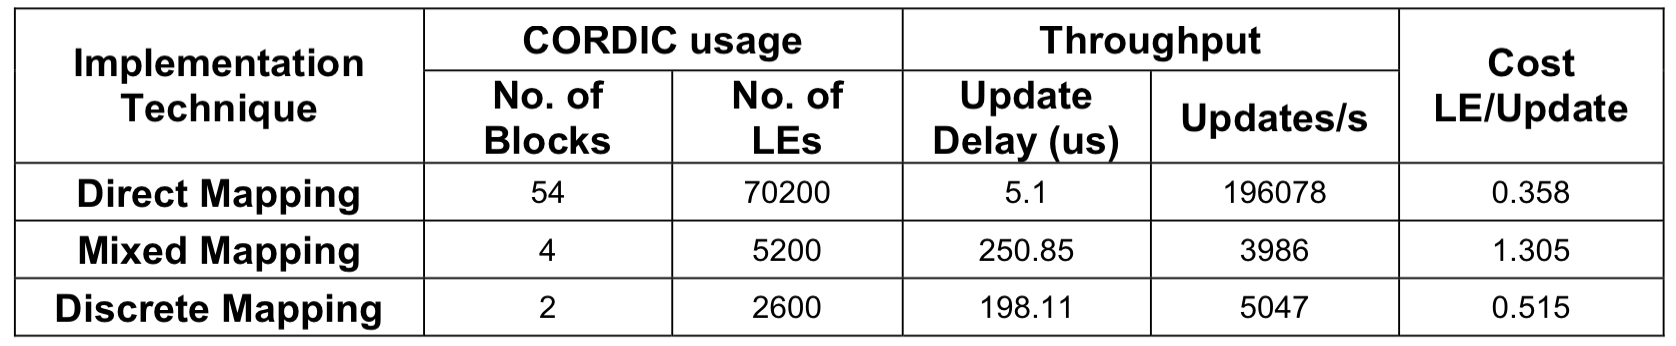
\includegraphics[width=12cm]{./figures/C03-altera_table}
     \caption{Tabla de métricas del hardware de Altera}
     \label{fig:altera_table}
\end{figure}

Entre las diferentes métricas, se encuentran las siguientes:

\begin{itemize}
\item[] \textit{Update Delay}: Tiempo requerido antes de que todas las celdas en el arreglo sistólico sean actualizadas.
\item[] \textit{Throughpu}t: Número de matrices de entrada (cada una de $M \times N$) que son procesadas por segundo ($= 1/\text{\textit{update delay}}$).
\item[] \textit{Cost}: Número de celdas básicas LE\footnote{\label{LE}Logic Element: Los elementos lógicos son las unidades más pequeñas de lógica en la arquitectura de la familia de dispositivos FPGA Cyclone III de Altera.} que ocupan las celdas CORDIC.
\end{itemize}

\subsection{Publicación de Xilinx}

\begin{itemize}
\item[] \textbf{Título}: \textit{FPGA Implementation of Matrix Inversion Using QRD-RLS Algorithm} 
\item[] \textbf{Autor/es}: Marjan Karkooti, Joseph R. Cavallaro, Chris Dick. Center for Multimedia Communication, Department of Electrical and Computer Engineering, Rice University / Xilinx
\end{itemize}

Este trabajo \cite{XilinxQR} detalla la realización de un filtro de \textit{beamforming} y fue desarrollado por un laboratorio de investigación de Xilinx en conjunto con la Universidad Rice. Su hardware utiliza dos CORDICs en \textit{vectoring mode} para cada una de las \textit{boundary cells} y la arquitectura de los mismos, a diferencia del hardware de la presente tesis, es desenrollada.

Para las \textit{internal cells}, la rotación no es implementada en hardware a través de un módulo CORDIC, sino que utiliza \textit{multiply accumulate (MAC) functional units}. Se utiliza el dispositivo FPGA Virtex 4, el cual consta de un gran arreglo de unidades MAC referidas como \textit{DSP48 slices}. Según menciona el documento, utilizar los bloques embebidos DSP48 en reemplazo de un enfoque basado en CORDIC para las \textit{internal cells} reduce la latencia de esta fase de cómputo y minimiza la cantidad de tablas de lógica FPGA (\textit{look-up tables LUTs} y registros) requeridas para la implementación. De todas maneras, se considera importante destacar el contexto de dicho tamaño dado que la arquitectura CORDIC es desenrollada.

\begin{figure}[h!]
     \centering
     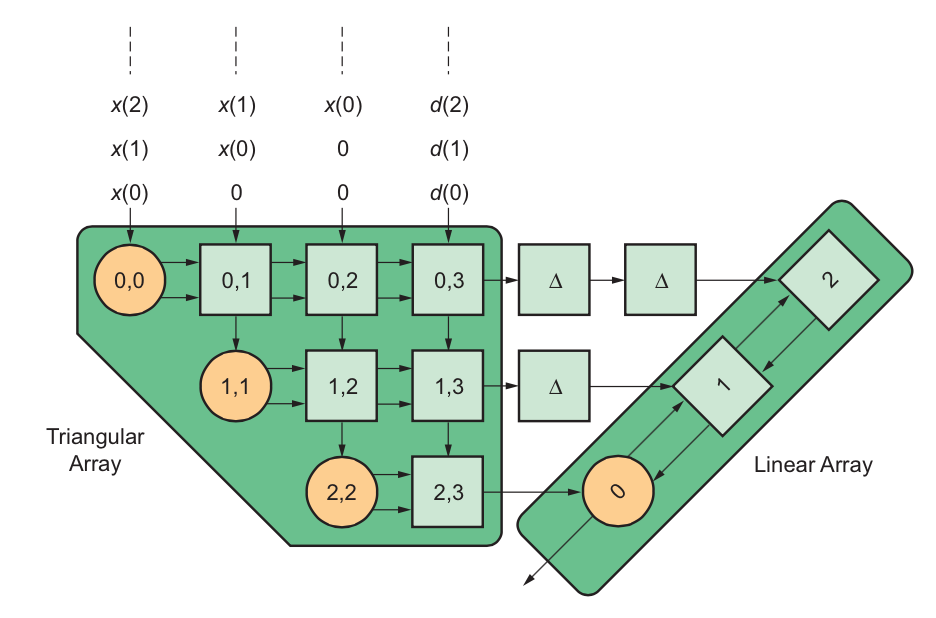
\includegraphics[width=12cm]{./figures/C03-xilinx_hardware}
     \caption{Arquitectura implementada por Xilinx}
     \label{fig:xilinx_hardware}
\end{figure}

Un dato interesante que presenta el trabajo para la comparativa es el tiempo requerido para el cálculo de la descomposición de una matriz utilizando varios valores de $M$ y $N$, entre los cuales se encuentra la matriz de $7 \times 7$. Sin embargo, no especifica la cantidad de bits de ancho de palabra utilizados.

Adicionalmente, detalla que se desarrolló un banco de pruebas con MATLAB. El script simula un objetivo dinámico y genera las muestras del patrón de radiación en campo lejano para el objetivo en movimiento. Las muestras del campo eléctrico en cada sensor se generan en MATLAB y son enviadas al procesador FPGA QRD. Se produce una nueva estimación del vector de peso conformador de haz y se envía a MATLAB para su posterior procesamiento.

\begin{figure}[h!]
     \centering
     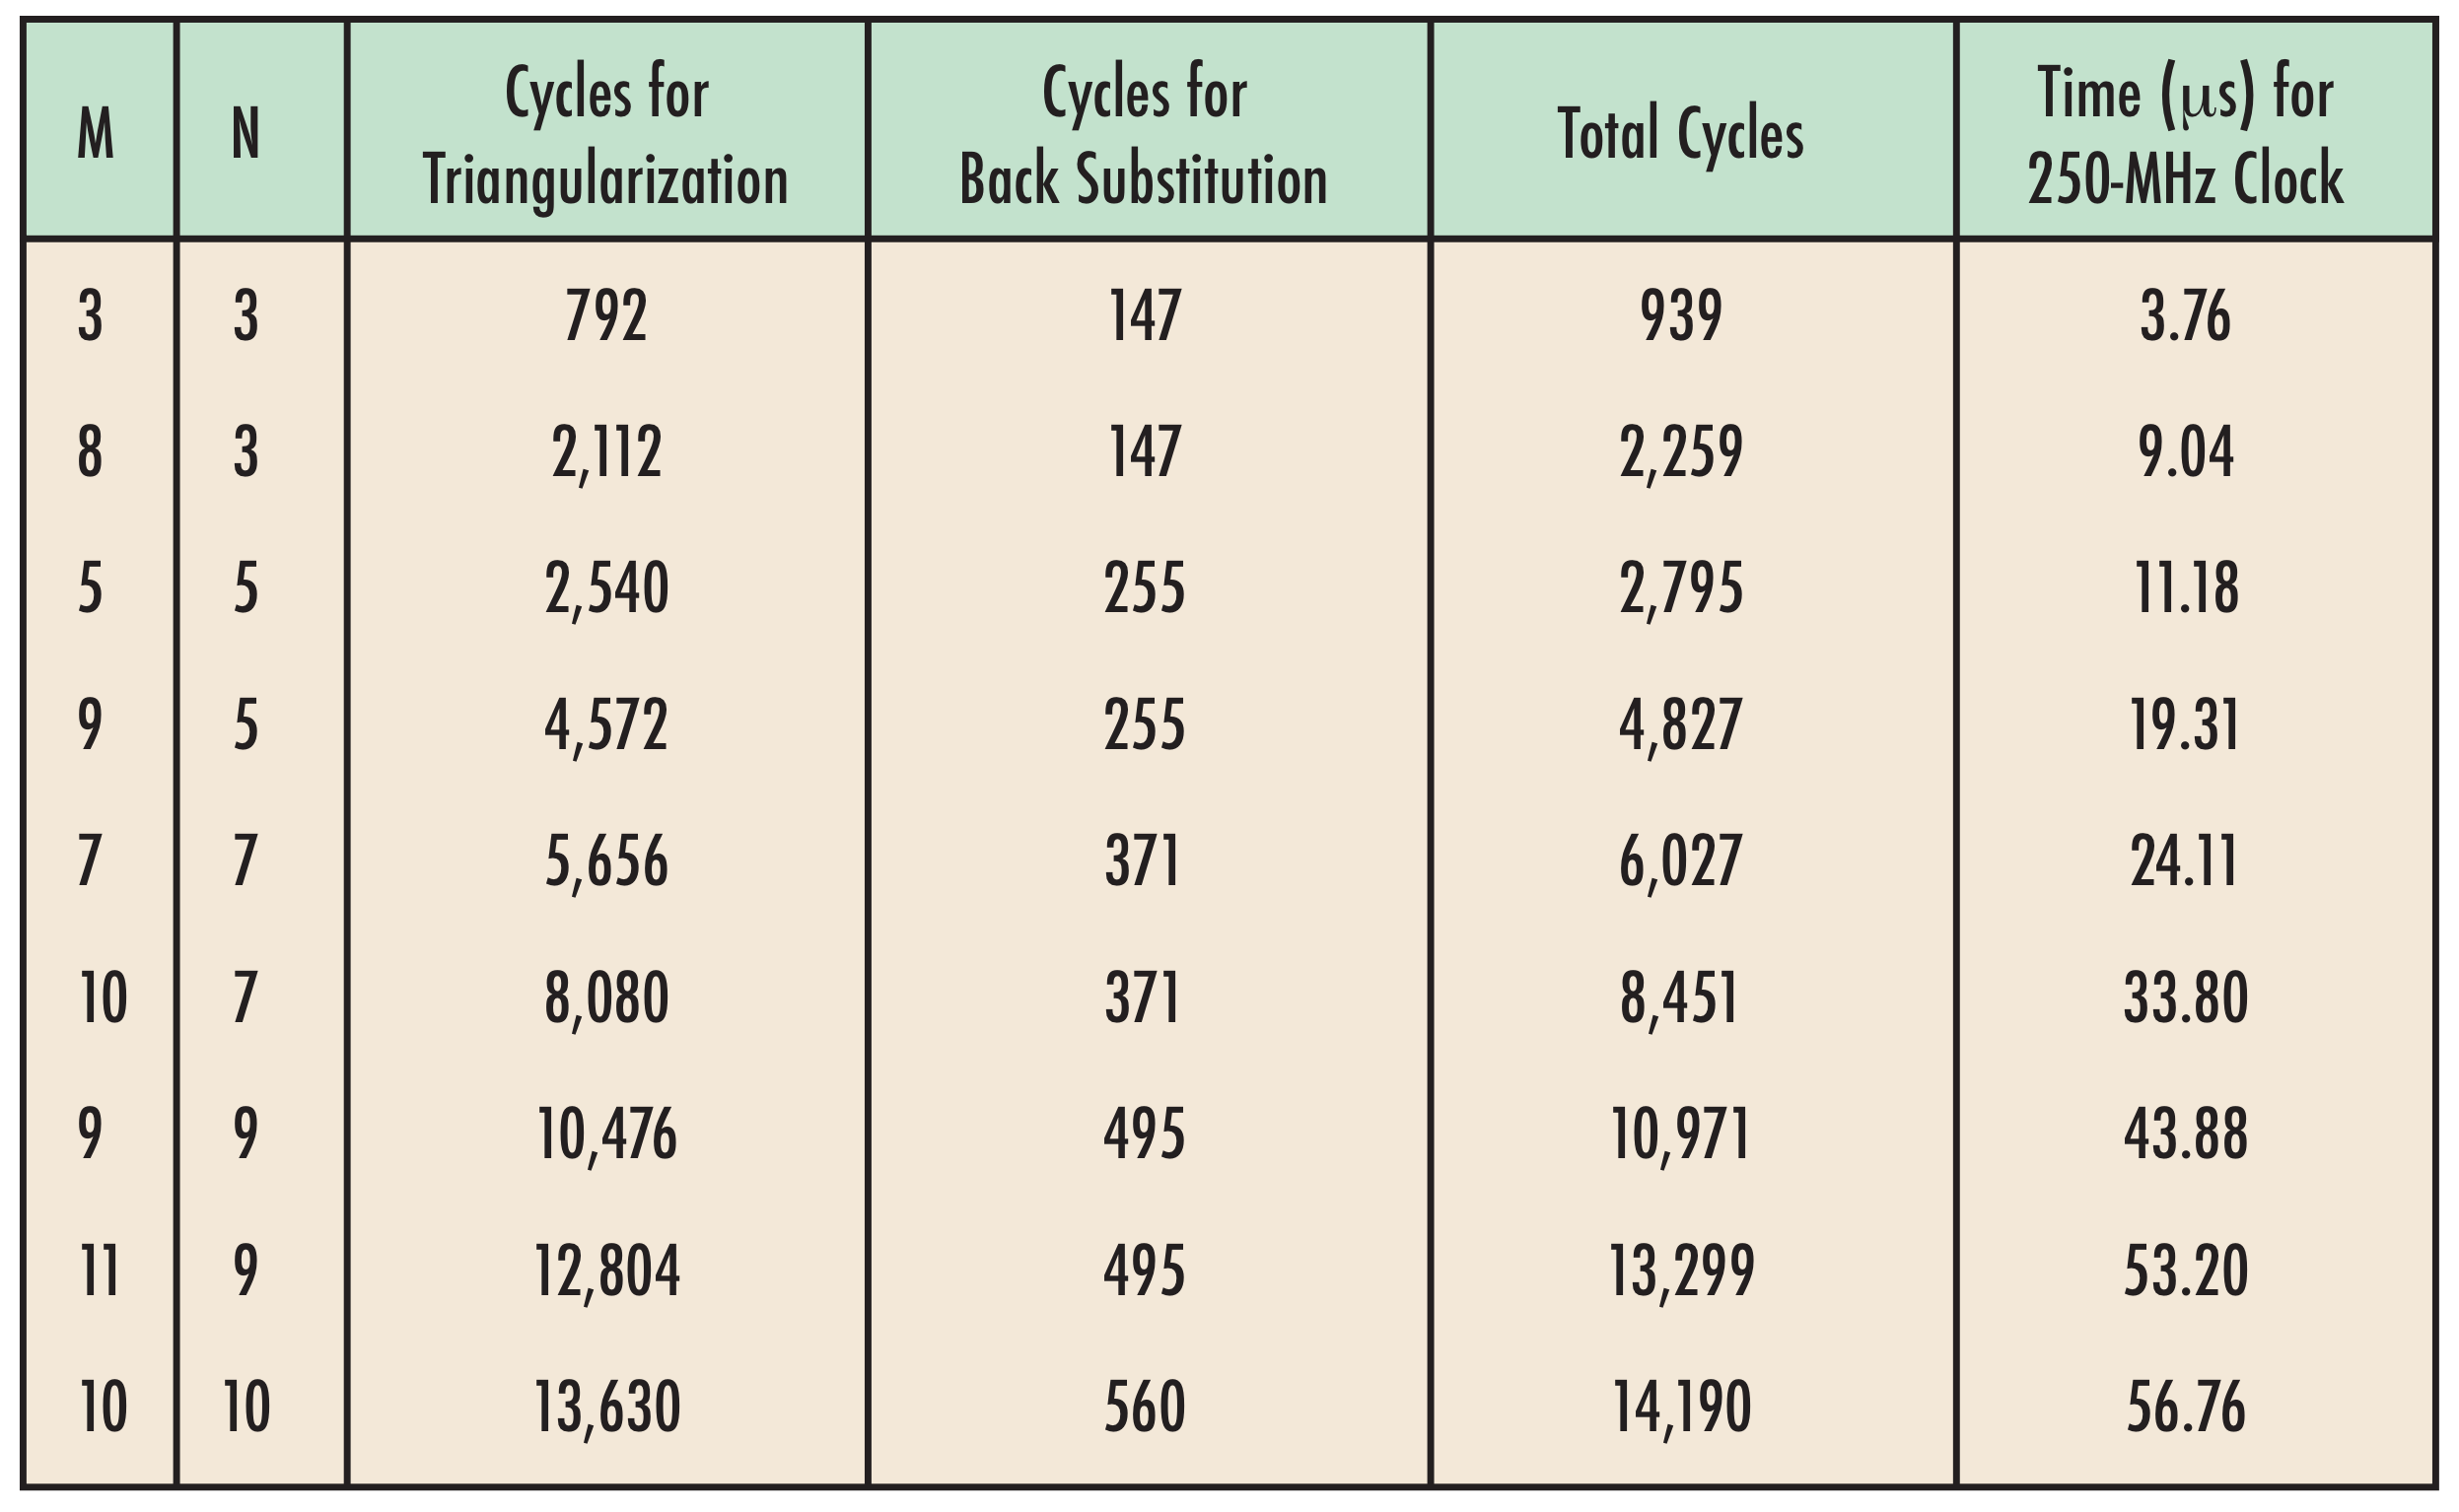
\includegraphics[width=12cm]{./figures/C03-xilinx_table}
     \caption{Tabla de métricas del hardware presentado por Xilinx}
     \label{fig:xilinx_table}
\end{figure}

\subsection{Publicación de Universidad de Victoria}

\begin{itemize}
\item[] \textbf{Título}: \textit{Fixed-Point CORDIC-Based QR Decomposition by Givens Rotations on FPGA}
\item[] \textbf{Autores}: Dongdong Chen, Mihai SIMA. Department of Electrical and Computer Engineering, University of Victoria
\end{itemize}

Este trabajo \cite{DongdongQR} contiene definiciones precisas sobre cómo fue desarrollado el hardware, cómo fue evaluado, y las diferentes métricas obtenidas. El hardware consta de un procesador de descomposición QR para matrices de $4 \times 4$, con ancho de palabra variable. Se utilizó un \textbf{mapeo directo} para desarrollar la arquitectura QR, la cual consta de un total de $21$ procesadores CORDIC.

\begin{figure}[h!]
     \centering
     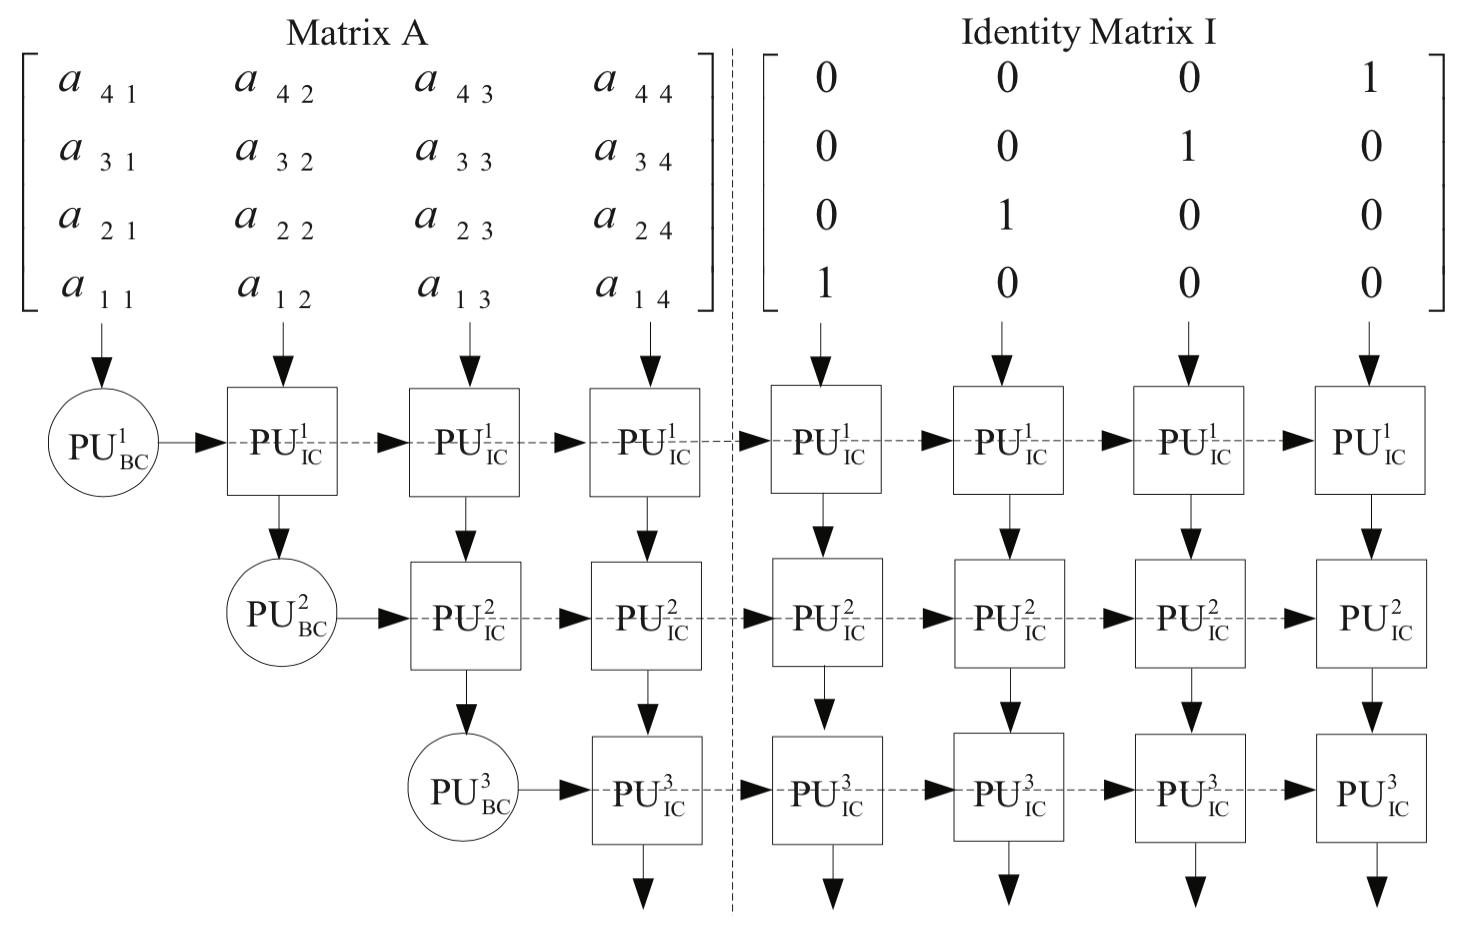
\includegraphics[width=8cm]{./figures/C03-dongdong_hardware}
     \caption{Arreglo de descomposición QR para una matriz de $4 \times 4$}
     \label{fig:dongdong_hardware}
\end{figure}

Una diferencia sustancial con la arquitectura que fue descripta, es que en ésta se agrega una sección de celdas/procesadores a derecha, la cual al ser inicializada con la matriz identidad, permite que al finalizar el cálculo se llegue al resultado de la matriz $Q^T$ (localizada en dichas celdas). Esta sección está compuesta por $3 \times 4 = 12$ celdas, siendo las $9$ celdas restantes utilizadas para el cálculo de la matriz $R$.

Se presenta un análisis teórico del \textit{timming} de la unidad, y una evaluación del error para diferentes anchos de palabra.

En forma similar al proyecto de Xilinx, desarrollaron un banco de pruebas basado en una simulación de MATLAB para contrastar resultados, utilizando un dispositivo FPGA Virtex 5 para realizar la síntesis, y sometiéndolo al cálculo de 100.000 matrices con elementos aleatorios.

Entre las métricas presentadas se encuentran distintos parámetros de evaluación del error, número de \textit{slices} ocupados, \textit{delay} de camino crítico, tiempo de procesamiento y \textit{throughput}.

\begin{figure}[h!]
     \centering
     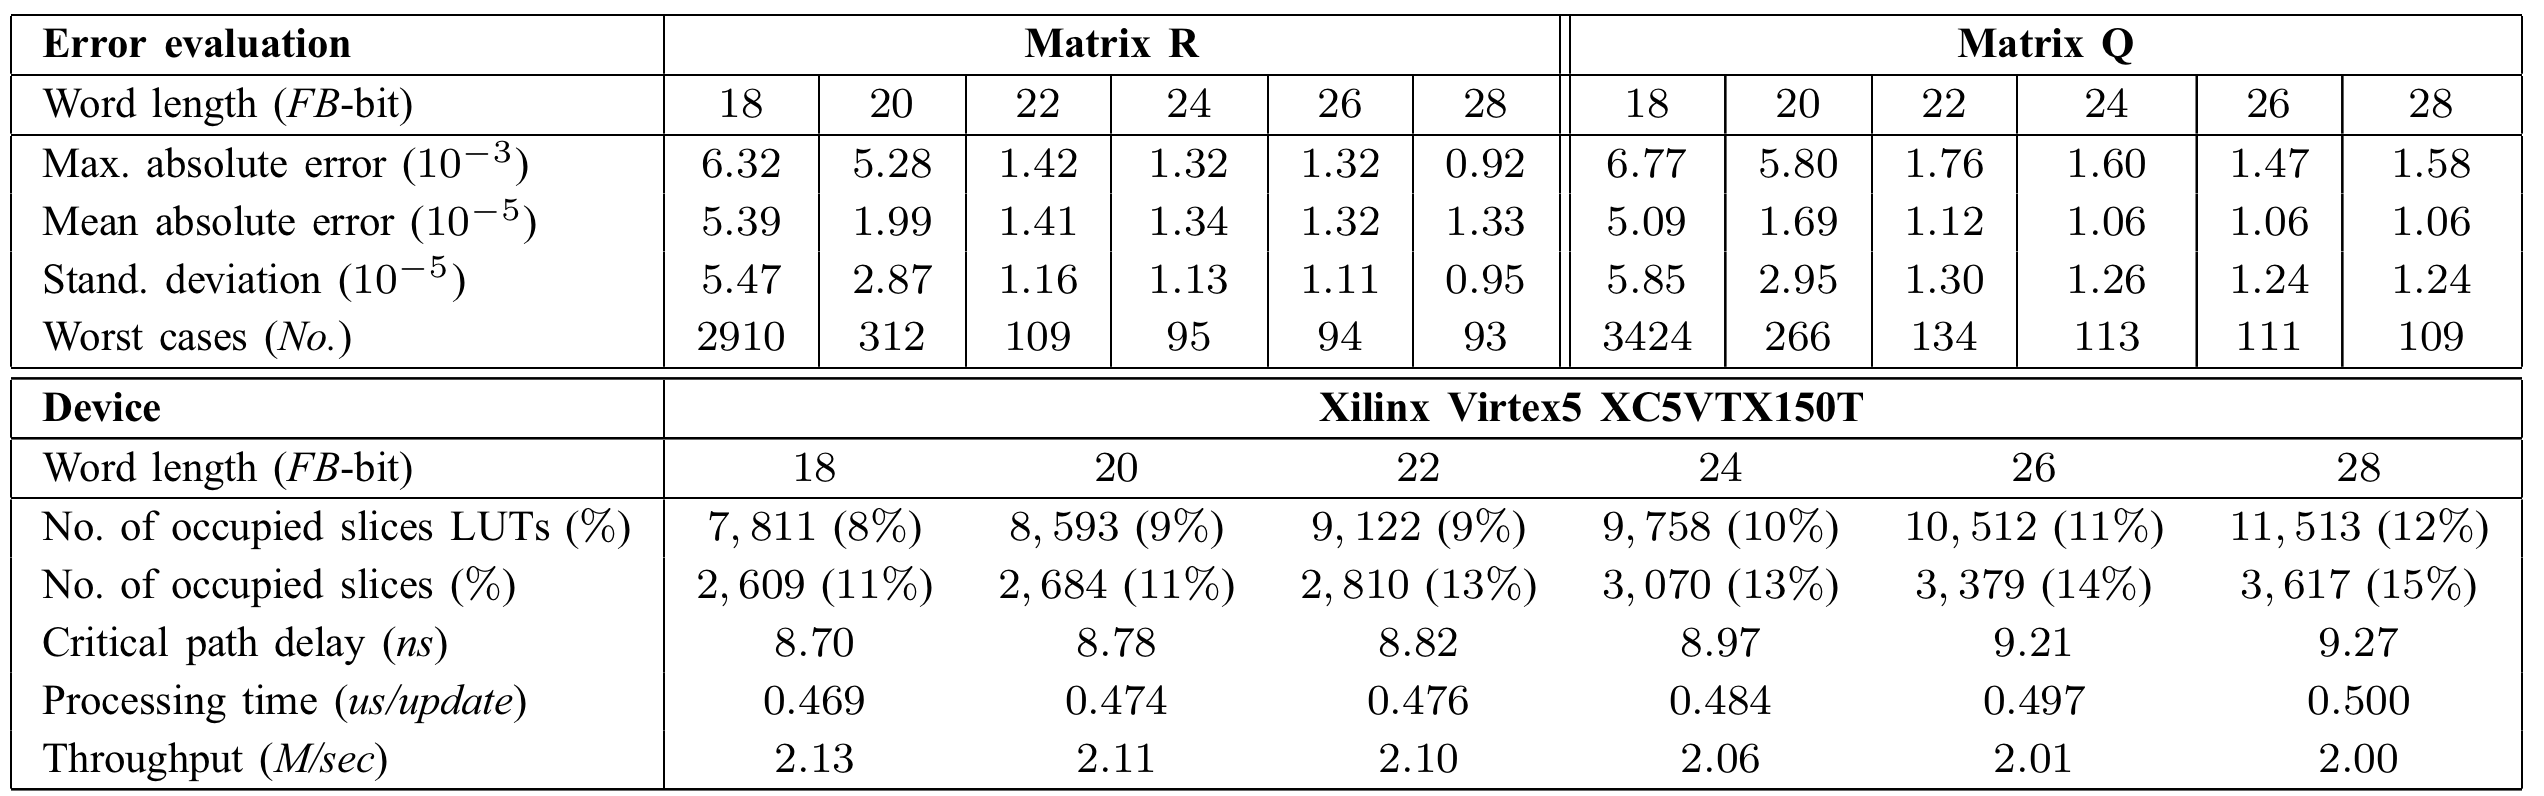
\includegraphics[width=14cm]{./figures/C03-dongdong_table}
     \caption{Tabla de métricas del hardware presentado}
     \label{fig:dongdong_table}
\end{figure}

\section{Arquitectura implementada}

La elección de la implementación utiliza RLS-QRD (algoritmo RLS a través de descomposición QR) como el sistema central para calcular adaptativamente los pesos del filtro.

A continuación se definen las premisas de la arquitectura elegida para la implementación del procesador de descomposición QR, sobre la cual se hará hincapié en el próximo capítulo:

\begin{itemize}
\item[•] \textbf{Tipo de Algoritmo:} Algoritmo Recursive Least Squares a través de descomposición QR.
\item[•] \textbf{Tipo de Rotaciones:} Rotaciones de Givens.
\item[•] \textbf{Hardware de Rotación:} CORDIC iterativo.
\item[•] \textbf{Cantidad de Procesadores de Celdas:} 4 módulos CORDIC.
\item[•] \textbf{Distribución de Celdas:} Mapeo de Walke \cite{Walke}.
\item[•] \textbf{Dimensión de la matriz:} $7 \times 7$.
\item[•] \textbf{Ancho de Palabra:} Hasta 64 \textit{bits}.
\end{itemize}
\chapter{Implementación a nivel de microarquitectura}

En el capítulo anterior se analizaron diferentes tipos de arquitecturas existentes para la implementación de un procesador de descomposición QR. Se describieron sus características a nivel conceptual y se detallaron las definiciones de la arquitectura elegida para realizar la implementación.

En este capítulo se describen las herramientas que fueron utilizadas y se explica en detalle, a nivel de microarquitectura, la forma en la cual fue implementado cada módulo del procesador desarrollado, y la forma en la cual los módulos fueron interconectados para conformar al mismo. Adicionalmente, se describen aquellos desarrollos que fueron el resultado de la presente tesis, utilizados para resolver diferentes necesidades encontradas, los cuales representan un contenido intelectual propio.

La metodología utilizada para el desarrollo del procesador consistió en analizar las necesidades de la arquitectura elegida, y los diferentes componentes requeridos. Se procedió a la definición de dicha arquitectura a través de un diagrama en bloques y se desarrolló cada uno de los módulos por separado, gradualmente. Una vez desarrollado un módulo, se procedió a simular su comportamiento aislado a través de un \textit{testbench} que lograra contemplar el mayor conjunto de los posibles vectores de entrada. Una vez finalizada la simulación individual de los distintos componentes, se procedió a realizar una simulación conjunta de algunos de ellos.

El detalle del código fuente Verilog puede encontrarse en el \autoref{cap:apA}.

\section{Diagrama en bloques}

A continuación se expone un diagrama en bloques a grandes rasgos del hardware desarrollado:

\begin{figure}[!h]
 	\begin{center}
 		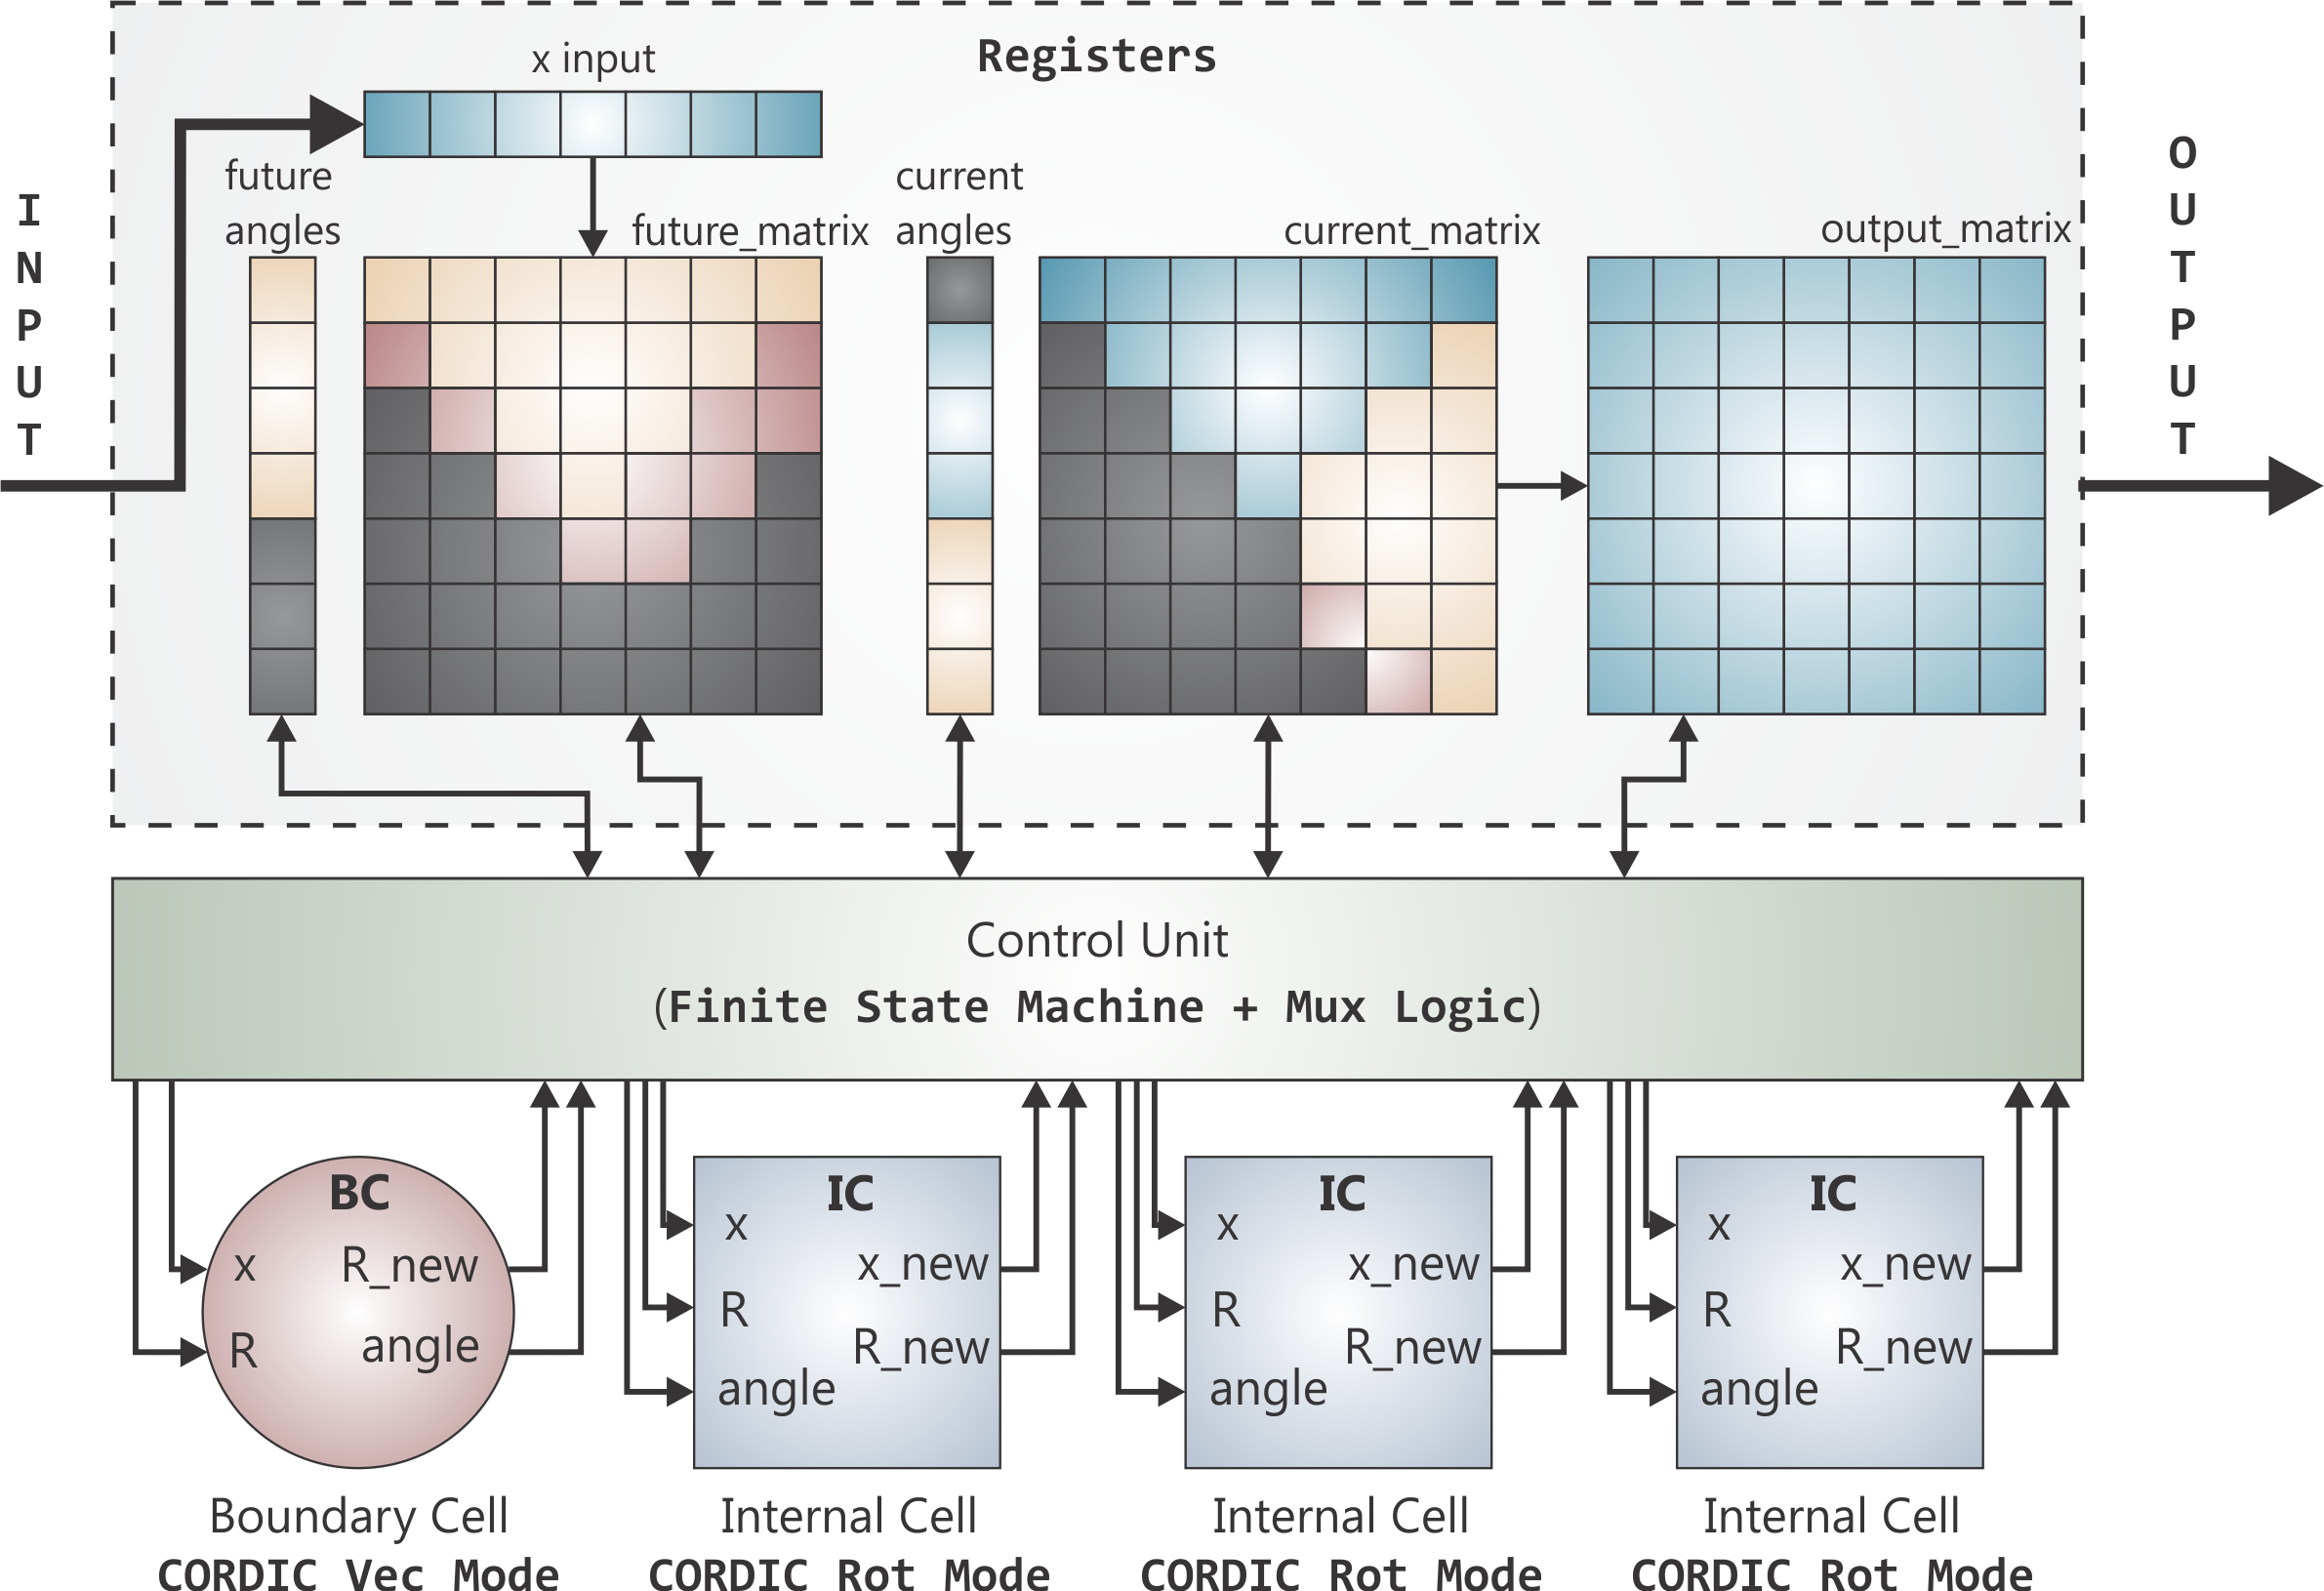
\includegraphics[width=\textwidth]{./figures/C04-block_diagram}
 		\caption{Diagrama en Bloques del Hardware Desarrollado}
		\label{block_diagram}
 	\end{center}
\end{figure}

En el diagrama se pueden observar las unidades desarrolladas para implementar la arquitectura elegida. Las mismas pueden dividirse en 3 grupos:

\begin{itemize}
	\item[•] La unidad de registros contiene el hardware requerido para almacenar los valores de entrada y salida de los procesadores, registrando cada uno de los cálculos realizados. Los datos se encuentran organizados en formato matricial. La unidad fue cuidadosamente desarrollada para adaptarse al comportamiento multiprocesamiento de la arquitectura, y para realizar operaciones de desplazamiento requeridas durante el procesamiento del algoritmo.

	\item[•] La unidad de control es el bloque de hardware que implementa la lógica necesaria para llevar a cabo los pasos del algoritmo según el mapeo de Walke, teniendo en cuenta el vector y las líneas de planificación. Esto se logra a partir del uso de una máquina de estados finita y multiplexores, para direccionar adecuadamente, según el estado actual, las entradas y salidas del hardware.
	
	\item[•] Los procesadores de \textit{boundary cell} e \textit{internal cell} son implementados utilizando núcleos CORDIC. En el caso de las operaciones BC, se utiliza CORDIC en \textit{vectoring mode}, y en el caso de las operaciones IC, el modo utilizado es \textit{rotation mode}. La \textit{boundary cell} es la unidad que toma como entrada los valores de $R$ y $x$ y realiza la rotación de los mismos para obtener el módulo del vector, el cual representa el nuevo valor de $R$, y el ángulo del mismo, el cual es utilizado para enviarlo como entrada a las \textit{internal cells} de la misma fila. Por otro lado, las \textit{internal cells} toman como entrada los valores de $R$, $x$, y el ángulo calculado por las \textit{internal cells}, para dar como resultado el nuevo valor de $R$, y el valor de $x$ para enviar como entrada a la \textit{internal cell} de la siguiente fila.
\end{itemize}

La descripción individual de cada uno de los componentes, empezando desde los módulos más básicos y continuando hasta evolucionar en el \textit{top level}, se encuentra en las siguientes secciones.

\section{Parámetros comunes a los distintos módulos}

\begin{itemize}
	\item[•] \verb;WORD_WIDTH;: Es el parámetro utilizado para definir el ancho de palabra de los datos que representan cada componente de la matriz. El valor por defecto es 16 \textit{bits} y puede soportar hasta 64. El número de iteraciones depende directamente de este valor, por lo cual al aumentar la precisión, aumenta el tiempo de procesamiento requerido.
	\item[•] \verb;ROWS;: Es el parámetro con el cual se define la cantidad de filas de la matriz. Actualmente, la implementación sólo admite que este valor sea 7.
	\item[•] \verb;COLUMNS;: Es el parámetro con el cual se define la cantidad de columnas de la matriz. Actualmente, la implementación sólo admite que este valor sea 7.
\end{itemize}

\section{Pre-procesamiento de entradas para el módulo CORDIC}

El código \textbf{preprocessor.v} describe el hardware desarrollado para hacer el pre-procesamiento de las entradas $x$;$y$;$z$ requerido, antes de enviarlas al procesador CORDIC. Es la primera etapa del módulo de rotación ``\textit{rotator}''. Según fue descripto en la sección \ref{subsec:El_algoritmo_CORDIC}, el procesador CORDIC sólo puede manejar rotaciones entre $-\pi/2$ y $\pi/2$ en cualquiera de sus dos modos de operación. Para aquellos casos en los cuales es necesario hacer rotaciones con ángulos mayores a $\pi/2$ en módulo, es requerido aplicar una rotación inicial de $\pi$.

En el modo rotación, esta transformación se logra negando ambas entradas, $x$ e $y$, y enviándolas al procesador CORDIC. Dicha transformación logra la rotación inicial de $\pi$ deseada, siendo la rotación restante manejada por el procesador CORDIC.  El resultado correcto es extraído directamente desde las salidas del mismo.

En el modo vector, es necesario abordar la transformación desde dos bloques distintos.
En primer lugar, se detecta si el vector de entrada posee un ángulo mayor a $\pi/2$ en módulo observando el signo de la componente $x$. Un ejemplo de dicho caso podría ser el vector $(-1000;1000)$. Estos casos se identifican cuando el signo de $x$ es negativo. En dicho caso, se aplica la misma transformación sobre $x$ e $y$ que se utilizó en el modo rotación, negando las componentes y enviándolas al modulo CORDIC.
En segundo lugar, se debe tomar el ángulo de salida de CORDIC $z_o$, y restarle $\pi$. Esta operación, es manejada por el módulo superior \textbf{rotator.v}.

Para realizar la implementación, se utiliza un \textit{bit} de decisión, el cual según el modo de CORDIC elegido, define qué parámetro será utilizado para determinar si es necesario modificar las entradas:

\begin{lstlisting}[style=C]
vec_rot_n ? d_i <= x_in[WORD_WIDTH-1] : ^z_in[WORD_WIDTH:WORD_WIDTH-1];
\end{lstlisting}

Luego, con el bit de decisión se controlan las entradas x e y y z siguiendo la siguiente lógica:

\begin{lstlisting}[style=C]
Si d_i se encuentra en estado alto entonces
	/* Angulo fuera del dominio valido de CORDIC */
	Asignar x de CORDIC con -x_i y extender 1 bit el signo
	Asignar y de CORDIC con -y_i y extender 1 bit el signo
	Si el modo es rotacion:
		Asignar z de CORDIC con z_i - pi
	sino
		Asignar z de CORDIC con z_i
sino
	/* Angulo dentro del dominio valido de CORDIC */
	Asignar x de CORDIC con x_i y extender 1 bit el signo
	Asignar y de CORDIC con x_i y extender 1 bit el signo
	asignar z de CORDIC con z_i
\end{lstlisting}

Al observar el pseudocódigo es posible identificar que se extienden en un \textit{bit} las entradas del sistema. El motivo de dicha extensión se basa en que, debido a la ganancia de CORDIC, pueden darse casos de overflow para ciertas entradas, y así llegar a resultados erróneos. Para evitarlo, la solución elegida consistió en:

\begin{enumerate}
	\item Extender las entradas en un \textit{bit} en la etapa de pre-procesamiento.
	\item Realizar el cálculo de CORDIC.
	\item Atenuar la ganancia de CORDIC en el módulo de post multiplicación.
	\item Eliminar el \textit{bit} de signo.
\end{enumerate}

De esta forma se adecúa el tamaño de las entradas del procesador CORDIC, evitando la posibilidad de llegar a una condición de overflow.

\section{CORDIC iterativo}

El código \textbf{iterative\_cordic.v} describe el hardware desarrollado para implementar el algoritmo de CORDIC según se encuentra descripto en el \autoref{cap:apC} en su versión iterativa. Lo que se requiere es lograr un hardware que replique las ecuaciones planteadas en \ref{ec3}. La composición del hardware se encuentra diagramada en la figura \ref{fig:cordic_hardware} y se logra como sigue:

\begin{itemize}
\item[•] Por un lado, se tiene un contador que registra el número de iteración dentro del algoritmo. La cantidad de cuentas de dicho contador depende directamente del ancho de palabra utilizado.
\item[•] Se utiliza un \textit{bit} de decisión \verb;di;, el cual trabaja utilizando el signo de $z$ o de $y$ según el modo sea rotación o vectorización.
\item[•] Cuando el hardware se encuentra en el estado \verb;IDLE;, las entradas $x$, $y$, $z$, ingresan en los registros de acumulación. Al salir del estado \verb;IDLE;, el acumulador es actualizado con el contenido de la salida del circuito en cada iteración. Está decisión es implementada por un multiplexor para cada componente $x$, $y$, $z$.
\item[•] $x$ e $y$, son direccionadas a registros de desplazamiento que operan según el número de iteración ( número de \textit{bits} desplazados = número de iteración).
\item[•] Se agregan dos circuitos \textit{add/substract} para implementar las dos ecuaciones de CORDIC. La elección de suma o resta es regida por el \textit{bit} de decisión. Los términos para cada uno son ($x$;$y$ desplazado) por un lado, e ($y$;$x$ desplazado) por el otro.
\item[•] Los valores de arcotangentes elementales son almacenados en una ROM. El acceso a la misma es controlado por el contador de iteraciones del algoritmo. La representación binaria se logra al multiplicar los valores absolutos por una constante para normalizarlos. Se utilizó una constante que normaliza los valores de la tabla para una representación en 64 \textit{bits}, el cual es el máximo valor aceptado por el hardware. En caso de que se utilicen longitudes de palabra menores, se hace un desplazamiento de dichas constantes a derecha (dividir por $2^n$) una cantidad $n = 64 - \text{longitud de palabra}$.

\begin{table}[hp!]
    \begin{center}
    	\footnotesize
        \begin{tabular}{|c|c|c|}
        \hline  
        \textbf{Iteración} & \textbf{Valor de Arcotangente} & \textbf{Representación Decimal de 64 bits} \\
        \hline
			1   &   0,78539816339744800000000   &   4611686018427387904   \\ \hline
			2   &   0,46364760900080600000000   &   2722437224269746380   \\ \hline
			3   &   0,24497866312686400000000   &   1438461061161762076   \\ \hline
			4   &   0,12435499454676100000000   &   0730185295051043895   \\ \hline
			5   &   0,06241880999595740000000   &   0366509582986589657   \\ \hline
			6   &   0,03123983343026830000000   &   0183433460584072433   \\ \hline
			7   &   0,01562372862047680000000   &   0091739112965426259   \\ \hline
			8   &   0,00781234106010111000000   &   0045872355853501789   \\ \hline
			9   &   0,00390623013196697000000   &   0022936527896151662   \\ \hline
			10  &   0,00195312251647882000000   &   0011468307695752815   \\ \hline
			11  &   0,00097656218955931900000   &   0005734159316382967   \\ \hline
			12  &   0,00048828121119489800000   &   0002867080341756270   \\ \hline
			13  &   0,00024414062014936200000   &   0001433540256323779   \\ \hline
			14  &   0,00012207031189367000000   &   0000716770138842597   \\ \hline
			15  &   0,00006103515617420880000   &   0000358385070756387   \\ \hline
			16  &   0,00003051757811552610000   &   0000179192535545079   \\ \hline
			17  &   0,00001525878906131580000   &   0000089596267793400   \\ \hline
			18  &   0,00000762939453110197000   &   0000044798133899308   \\ \hline
			19  &   0,00000381469726560650000   &   0000022399066949980   \\ \hline
			20  &   0,00000190734863281019000   &   0000011199533475031   \\ \hline
			21  &   0,00000095367431640596100   &   0000005599766737520   \\ \hline
			22  &   0,00000047683715820308900   &   0000002799883368761   \\ \hline
			23  &   0,00000023841857910155800   &   0000001399941684380   \\ \hline
			24  &   0,00000011920928955078100   &   0000000699970842190   \\ \hline
			25  &   0,00000005960464477539060   &   0000000349985421095   \\ \hline
			26  &   0,00000002980232238769530   &   0000000174992710547   \\ \hline
			27  &   0,00000001490116119384770   &   0000000087496355274   \\ \hline
			28  &   0,00000000745058059692383   &   0000000043748177637   \\ \hline
			29  &   0,00000000372529029846191   &   0000000021874088818   \\ \hline
			30  &   0,00000000186264514923096   &   0000000010937044409   \\ \hline
			31  &   0,00000000093132257461548   &   0000000005468522204   \\ \hline
			32  &   0,00000000046566128730774   &   0000000002734261102   \\ \hline
        \end{tabular}
        \normalsize
        \caption{Tabla de Arcotangentes}
    \end{center}
\end{table}

\newpage

\item[•] La salida de z se implementa independientemente en forma similar a la de $x$ e $y$, sumando o restando ángulos según el \textit{bit} de decisión, pero tomando como segundo término de la suma/resta el valor de la ROM de arcotangentes, según el valor para la iteración correspondiente.
\end{itemize}

El diagrama del circuito de CORDIC implementado es el siguiente:

\begin{figure}[!h]
 	\begin{center}
 		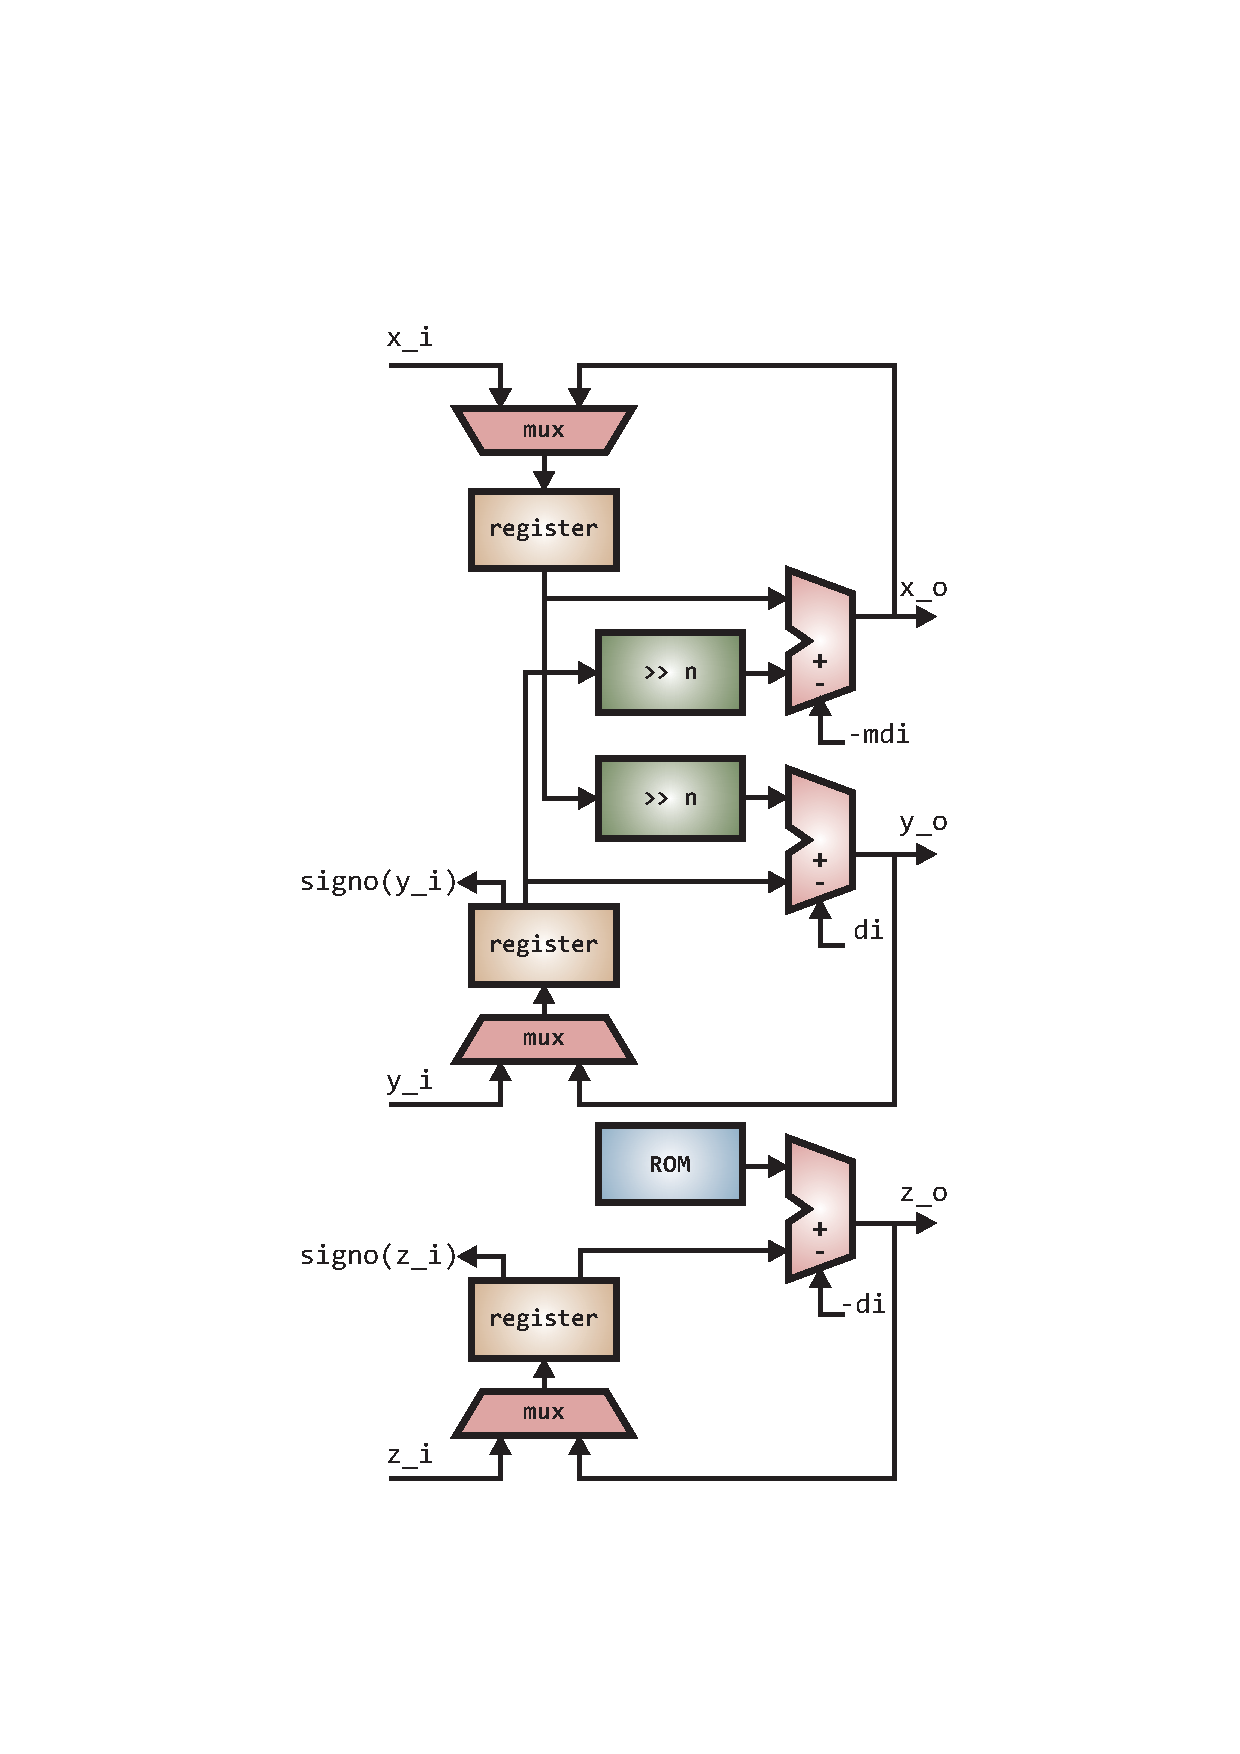
\includegraphics[width=7 cm]{./figures/C04-cordic_hardware}
 		\caption{Diagrama RTL de la implementación de CORDIC en hardware}
		\label{fig:cordic_hardware}
 	\end{center}
\end{figure}

\section{Post-multiplicador de salidas $x$ e $y$ de CORDIC}

El código \textbf{postmultiplier.v} describe el hardware desarrollado para hacer la atenuación requerida para compensar la ganancia de CORDIC. Es la última etapa del módulo de rotación ``\textit{rotator}'', y se aplica a las salidas de $x$ e $y$ de CORDIC. Según fue descripto en la sección \ref{subsec:El_algoritmo_CORDIC}, el hardware CORDIC introduce una ganancia $A_n$ al aplicar la rotación. Como en el hardware implementado es requerido que los vectores rotados no se vean escalados por la misma, se debe implementar una post-multiplicación que la atenúe.

Para implementar dicha multiplicación se hizo uso de la primitiva de producto del lenguaje Verilog, siendo la implementación definida al momento de la síntesis.

\section{Unidad de rotación completa}

El código \textbf{rotator.v} describe el hardware desarrollado para implementar un rotador el cual, utilizando los módulos de CORDIC, pre-procesamiento y post-multiplicación, sea capáz de manejar las operaciones BC e IC correctamente, sin importar el ángulo de los vectores de entrada (conformados por los valores de $R$ y $x$) y sin producir escalamientos. Para lograrlo, dicho hardware instancia un pre-procesador, un módulo CORDIC iterativo, dos post-multiplicadores (uno para $x$ y otro para $y$), y adicionalmente contiene el hardware de ajuste de ángulo requerido para los casos en que se utilice el modo vectorización y el vector de entrada tenga un ángulo mayor $\pi/2$ en módulo.

A continuación se expone un diagrama en bloques de la composición del rotador:

\begin{figure}[!h]
 	\begin{center}
 		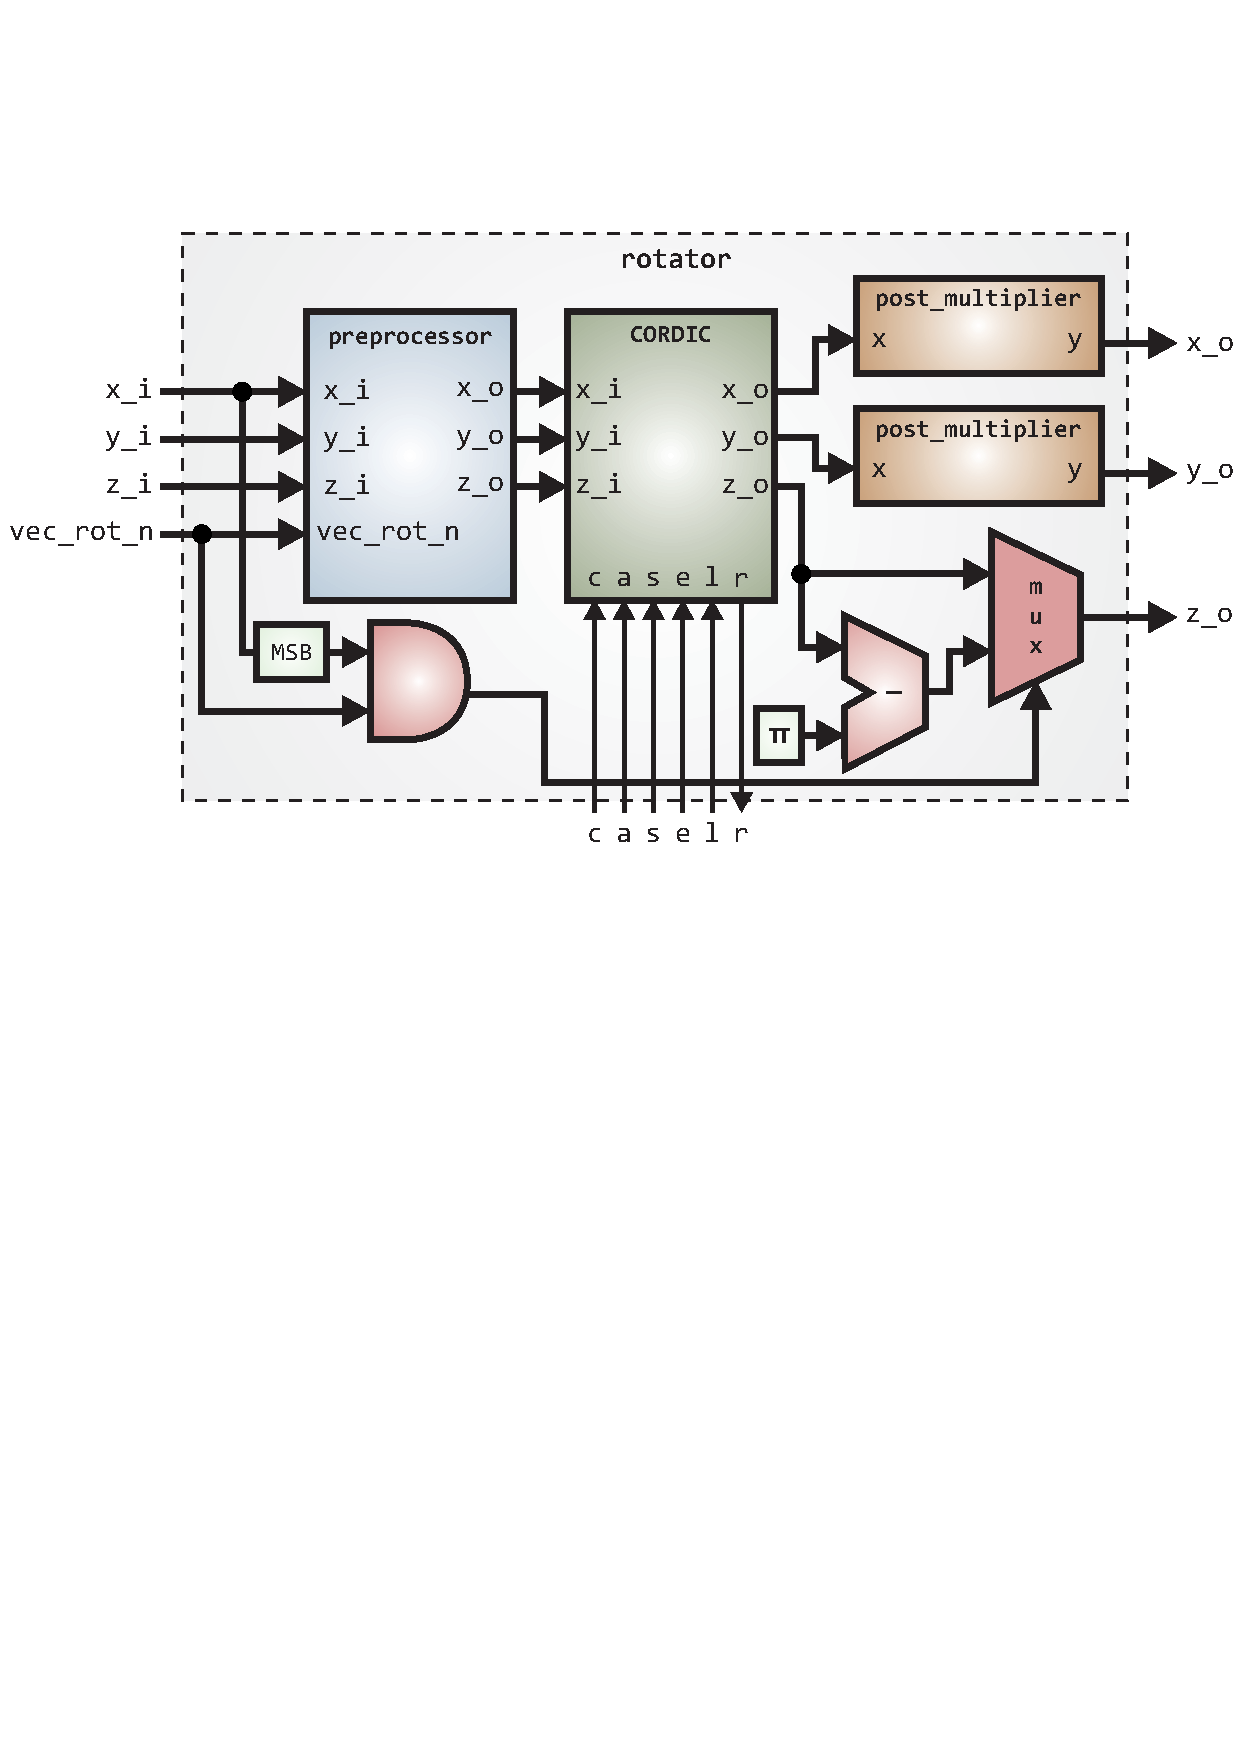
\includegraphics[width=15 cm]{./figures/C04-rotator_diagram}
 		\caption{Diagrama en Bloques del Módulo de Rotación}
		\label{rotator_diagram}
 	\end{center}
\end{figure}

\section{Procesador boundary cell}

El código \textbf{boundary\_cell.v} describe el hardware desarrollado para implementar las operaciones BC del procesador de descomposición QR. Las mismas fueron descriptas en la sección \ref{sec:descomposicion_qr} y se rigen por las ecuaciones \ref{eq:boundary_cell_1}, \ref{eq:boundary_cell_2} y \ref{eq:boundary_cell_3}. Para lograr la implementación de dichas ecuaciones, en el mismo se instancia un módulo rotador y se direccionan adecuadamente los valores de $R$ y $x$ de entrada, y los valores de $R_{new}$ y $angle$ de salida. El modo de operación del rotador se define de forma constante como modo vectorización.

\section{Procesador internal cell}

El código \textbf{internal\_cell.v} describe el hardware desarrollado para implementar las operaciones IC del procesador de descomposición QR. Las mismas fueron descriptas en la sección \ref{sec:descomposicion_qr} y se rigen por las ecuaciones \ref{eq:internal_cell_1} y \ref{eq:internal_cell_2}. Para lograr la implementación de dichas ecuaciones, en el mismo se instancia un módulo rotador y se direccionan adecuadamente los valores de $R$, $x$ y $angle$ de entrada, y los valores de $R_{new}$ y $x_{new}$ de salida. El modo de operación del rotador se define de forma constante como modo rotación.

\section{Procesador de descomposición QR}

El código \textbf{qr\_processor.v} es el \textit{top module} del proyecto y describe el hardware desarrollado para implementar el procesador de descomposición QR. A través de la definición de la unidad de registros, la lógica de control y la instanciación e interconexión de los módulos de celda que fueron descriptos, el mismo logra la implementación en hardware del algoritmo descripto.

La organización del código está distribuida como sigue:

\begin{enumerate}
	\item Definición del \textit{layout} del módulo, el cual incluye sus parámetros, entradas y salidas.
	\item Definición de los estados de control.
	\item Definición de registros e interconexiones.
	\item Instanciación de circuitos (\textit{boundary\_cell} e \textit{internal\_cell}).
	\item Definición de la arquitectura.
\end{enumerate}

\newpage

\subsection{Interfaz del módulo}

A continuación se describen las entradas y salidas del módulo:

\begin{itemize}
	\item[ ] \textbf{Entradas:}
	\item[•] \verb;clk;    : Entrada de \textit{clock} del sistema. El hardware opera por detección de flanco ascendente.
	\item[•] \verb;arst;   : \textit{Reset} asincrónico activo en alto.
	\item[•] \verb;srst;   : \textit{Reset} sincrónico  activo en alto.
	\item[•] \verb;enable; : \textit{Enable} sincrónico activo en alto.
	\item[•] \verb;start;  : \textit{Flag} para indicar que se está suministrando un nuevo vector de entrada, el cual dispara el cálculo para una nueva matriz R.
	\item[•] \verb;lambda_option; : Selector de factor de olvido.
	\item[•] \verb;x_in_1; : Primer elemento del vector de entrada.
	\item[•] \verb;x_in_2; : Segundo elemento del vector de entrada.
	\item[•] \verb;x_in_3; : Tercer elemento del vector de entrada.
	\item[•] \verb;x_in_4; : Cuarto elemento del vector de entrada.
	\item[•] \verb;x_in_5; : Quinto elemento del vector de entrada.
	\item[•] \verb;x_in_6; : Sexto elemento del vector de entrada.
	\item[•] \verb;x_in_7; : Séptimo elemento del vector de entrada.
\end{itemize}

\begin{itemize}   
	\item[ ] \textbf{Salidas:}
	\item[•] \verb;ready;      : Cuando se encuentra en estado alto, indica que el resultado se encuentra disponible. La matriz de salida va a ser enviada, de a una fila por ciclo de clock, en las salidas \verb;y_out; donde cada una de ellas representa cada columna.
	\item[•] \verb;y_out_1;    : Primera columna de la fila correspondiente de la matriz de salida.
	\item[•] \verb;y_out_2;    : Segunda columna de la fila correspondiente de la matriz de salida.
	\item[•] \verb;y_out_3;    : Tercera columna de la fila correspondiente de la matriz de salida.
	\item[•] \verb;y_out_4;    : Cuarta columna de la fila correspondiente de la matriz de salida.
	\item[•] \verb;y_out_5;    : Quinta columna de la fila correspondiente de la matriz de salida.
	\item[•] \verb;y_out_6;    : Sexta columna de la fila correspondiente de la matriz de salida.
	\item[•] \verb;y_out_7;    : Séptima columna de la fila correspondiente de la matriz de salida.
\end{itemize}

\subsection{Uso del procesador QR}

La implementación del procesador desarrollada es capáz de calcular la descomposición QR de una matriz de $7 \times 7$. La salida es la matriz $R$, la cual contiene la información requerida de la matriz de entrada. La matriz $Q$ forma una base ortogonal que al ser multiplicada por $R$ equivale a la matriz de entrada. 

Si bien es posible computar la matriz $Q$ haciendo uso de los ángulos de salida calculados en las \textit{boundary cells}, o agregando hardware de triangularización adicional, no se realiza dicha implementación dado que la misma no es requerida para la aplicación elegida, en la cual el objetivo es el cálculo del vector de pesos de un \textit{beamformer}.

En esta aplicación, las columnas de la matriz de entrada se generan por las últimas $7$ muestras de $6$ antenas (primeras $6$ columnas, vector $x$) y una secuencia de entrenamiento (última columna, elemento $y$).

Dado el carácter recursivo de la implementación, para suministrar la matriz de entrada es necesario hacerlo de a una fila por vez. Se comienza suministrando la primera fila, activando el \textit{flag} \verb;start;, y esperando a que la señal de ready se coloque en estado en alto antes de suministrar la próxima fila. Se presenta en la figura \ref{fig:hardware_use} un diagrama de tiempos al insertar una primera fila $A = [a_1\ a_2\ a_3\ a_4\ a_5\ a_6\ a_7]$. Dicho proceso se debería repetir con las 6 filas restantes de la matriz.

\begin{figure}[!h]
 	\begin{center}
 		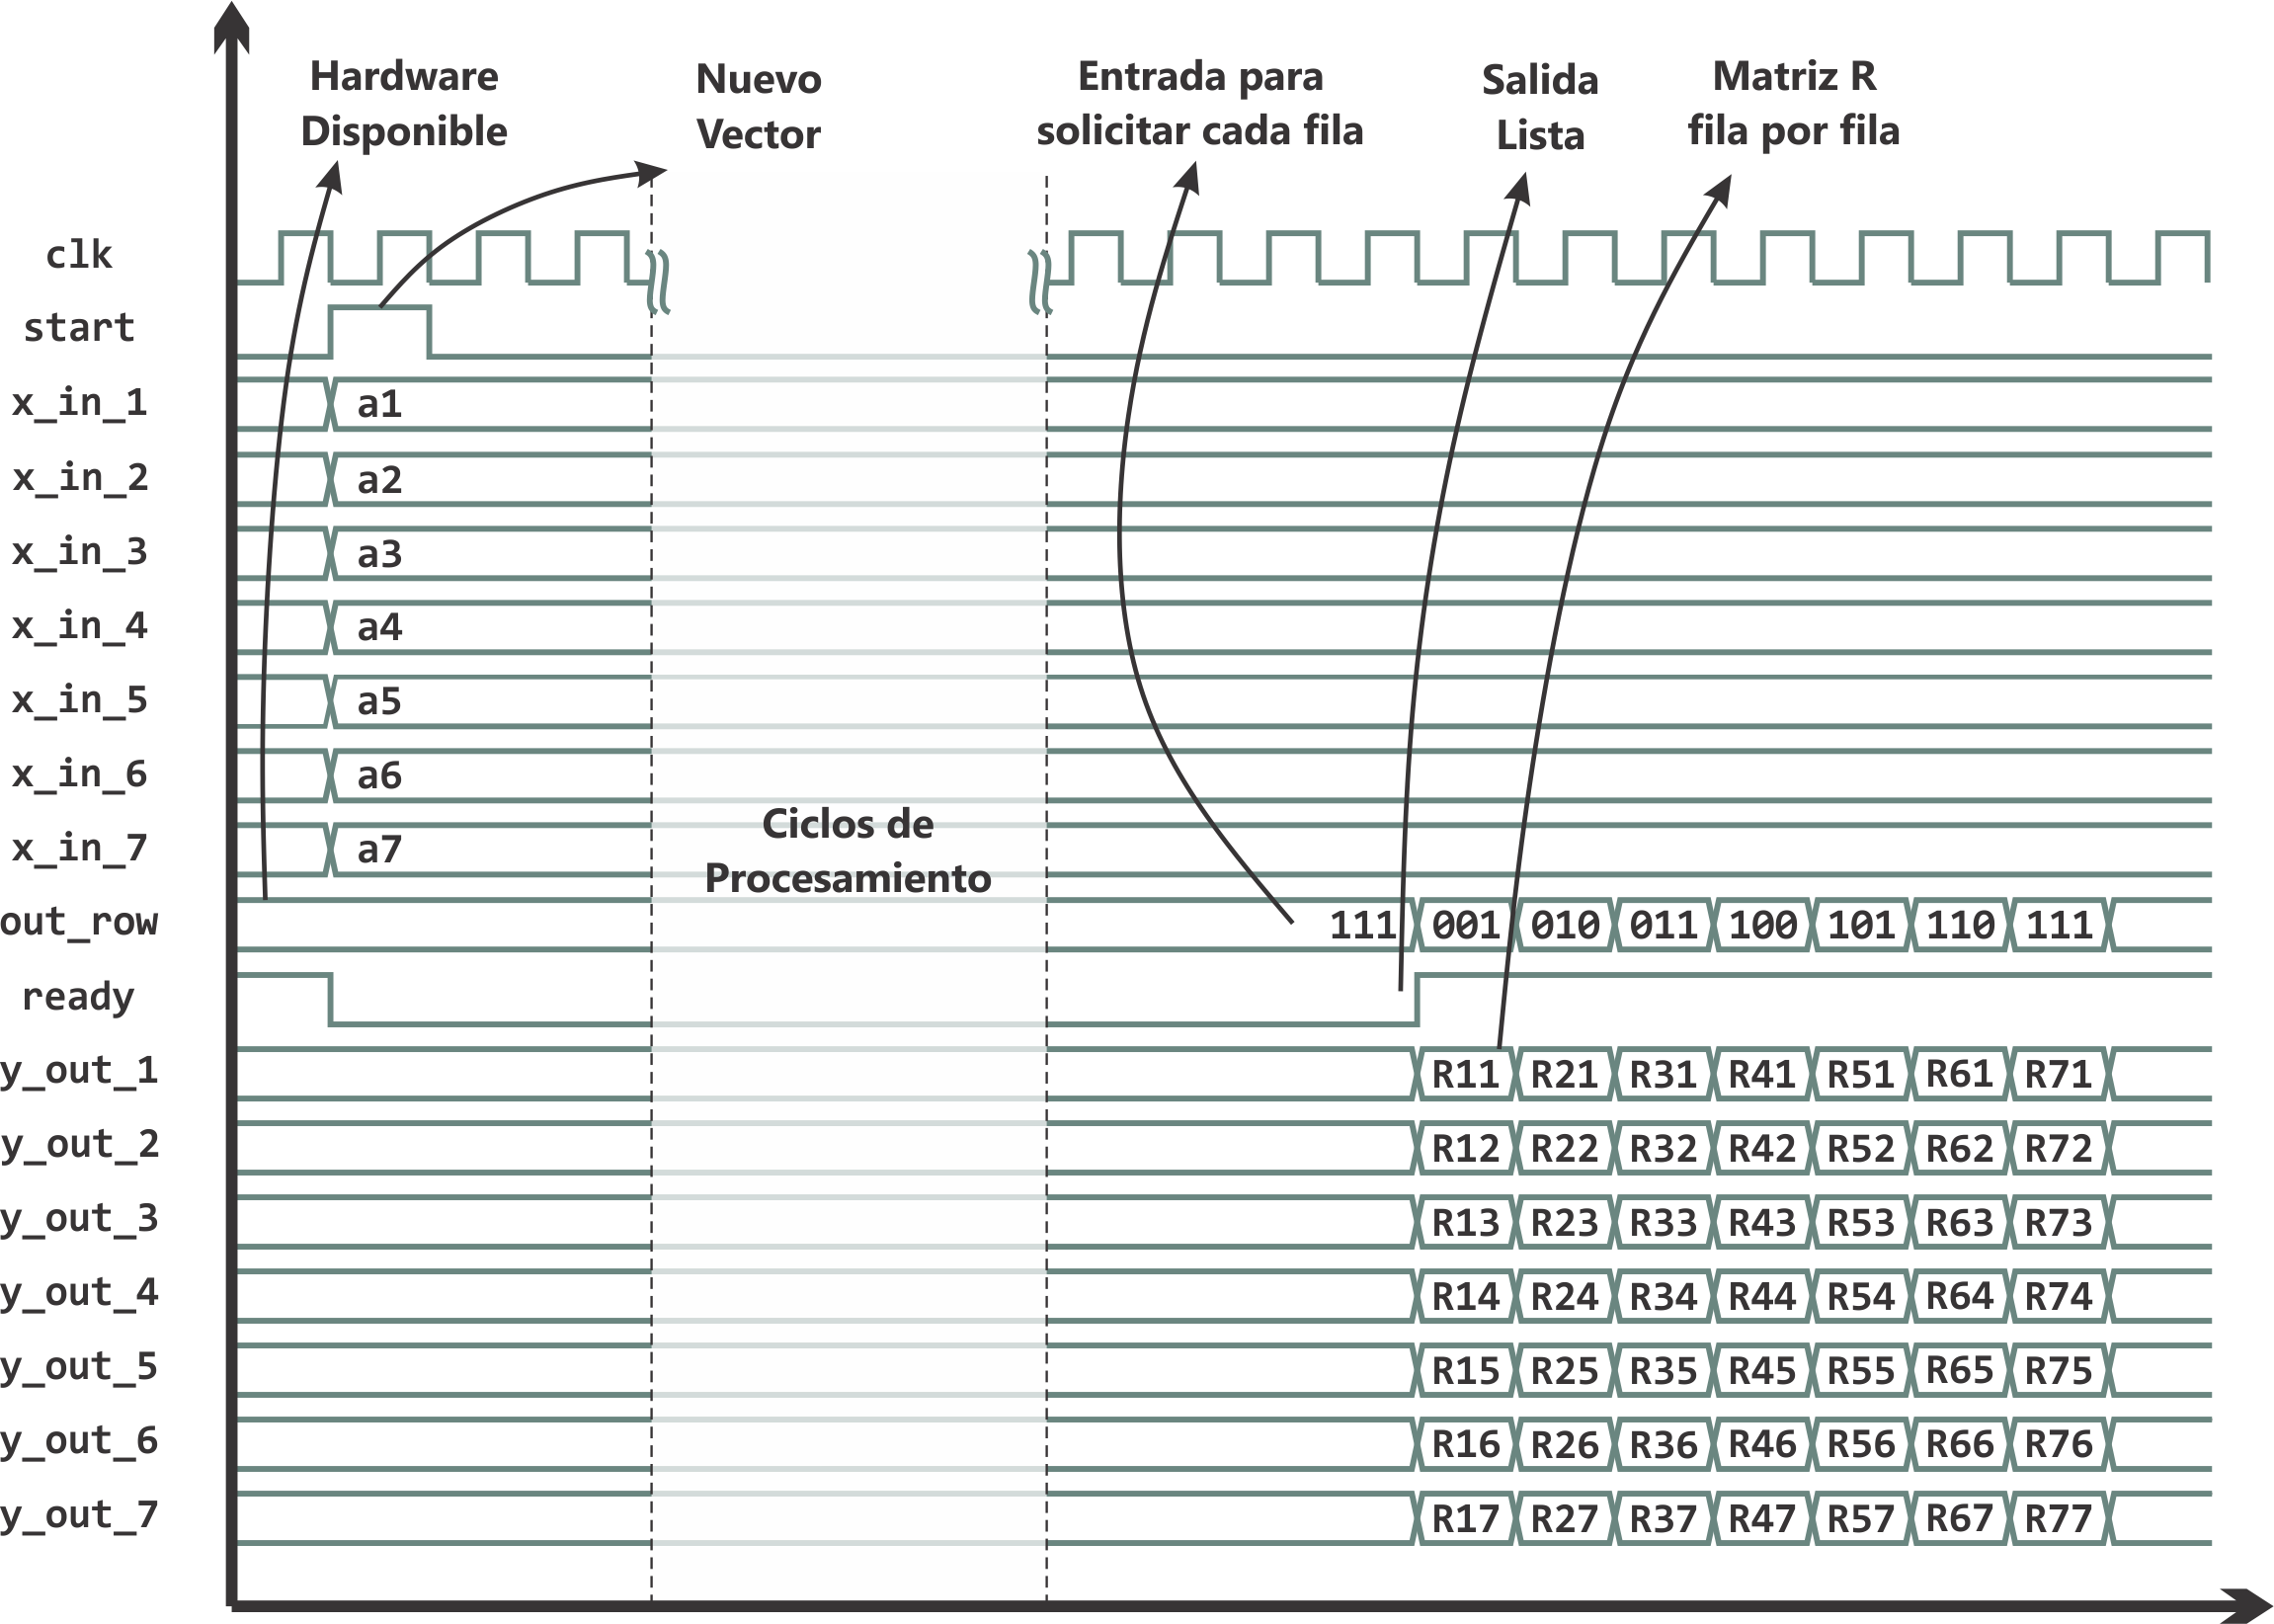
\includegraphics[width=11 cm]{./figures/C04-hardware_use}
 		\caption{Diagrama de Tiempos en el uso del Hardware}
		\label{fig:hardware_use}
 	\end{center}
\end{figure}

La composición de la matriz es siempre generada por un desplazamiento hacia abajo de las filas, en el cual se pierde la última fila, e ingresa en la primera el nuevo vector de entrada suministrado. Esta implementación recursiva se adapta al proceso de \textit{beamforming}, donde las filas que se mantienen representan las últimas 6 muestras. Este comportamiento se observa en la figura \ref{fig:hardware_cycles}. En la imagen se debe notar, por un lado el cambio en cada procesamiento, donde se observa el resultado anterior desplazado, y por el otro, la pérdida de la última fila en el Octavo Procesamiento.

\begin{figure}[!h]
 	\begin{center}
 		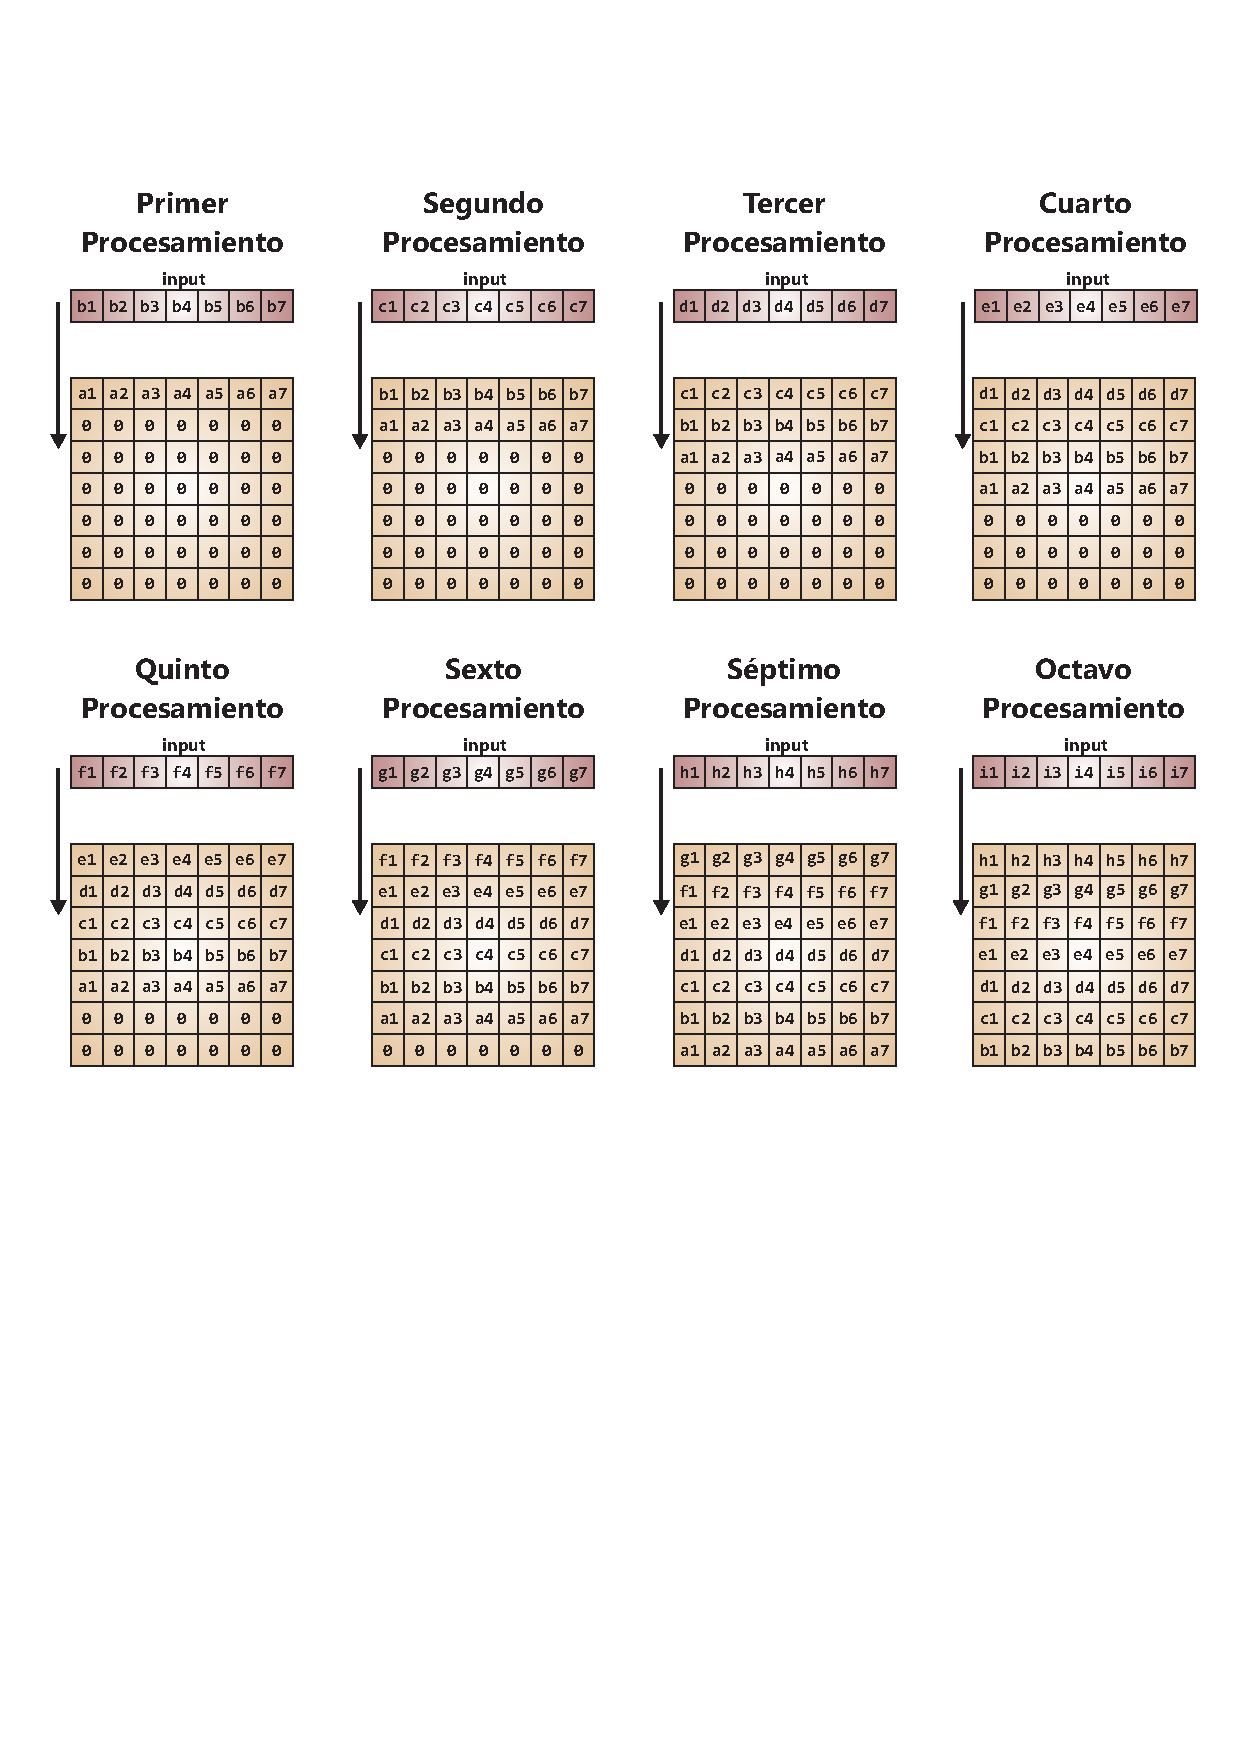
\includegraphics[width=13 cm]{./figures/C04-hardware_cycles}
 		\caption{Esquema de los primeros 8 ciclos de procesamiento}
		\label{fig:hardware_cycles}
 	\end{center}
\end{figure}

La matriz de entrada completa nunca es almacenada en los registros internos del procesador, dado que no es necesario contar con la misma. Si fuese un requerimiento, fácilmente se podría incorporar la misma en la unidad de registros desarrollada.

Si se deseara calcular una matriz completamente nueva, se debe repetir el proceso de suministrar cada fila esperando a que se active la señal de \textit{ready}.

\newpage

\subsection{Unidad de registros}

A continuación se hará una descripción detallada de la forma en la cual se almacenan y utilizan los elementos de una matriz en hardware. En la sección \ref{subsec:mapeo_de_walke}, se explicó que es necesario retener los valores de $R$ de una iteración, para la siguiente. En el mapeo de Walke, al reducir la arquitectura, se requiere que no sólo los valores de $R$ se almacenen, sino también los de $x$, y al ser varios pares $(x,R)$ asignados a un mismo procesador, esto es requerido para varios ciclos.

Esta implementación podría haber sido realizada dentro de las celdas, pero en lugar de hacerlo de esta forma, se optó por crear una unidad de registros, que tenga ciertas propiedades particulares para dar ventajas a la ejecución del algoritmo. Tanto la unidad de registros, como la forma en la cual se opera, es un diseño propio que presenta diversas ventajas para el mapeo, y fue ideado específicamente durante el desarrollo.

Como se vio en el diagrama en bloques, el esquema de almacenamiento de datos es el siguiente:

\begin{figure}[!h]
 	\begin{center}
 		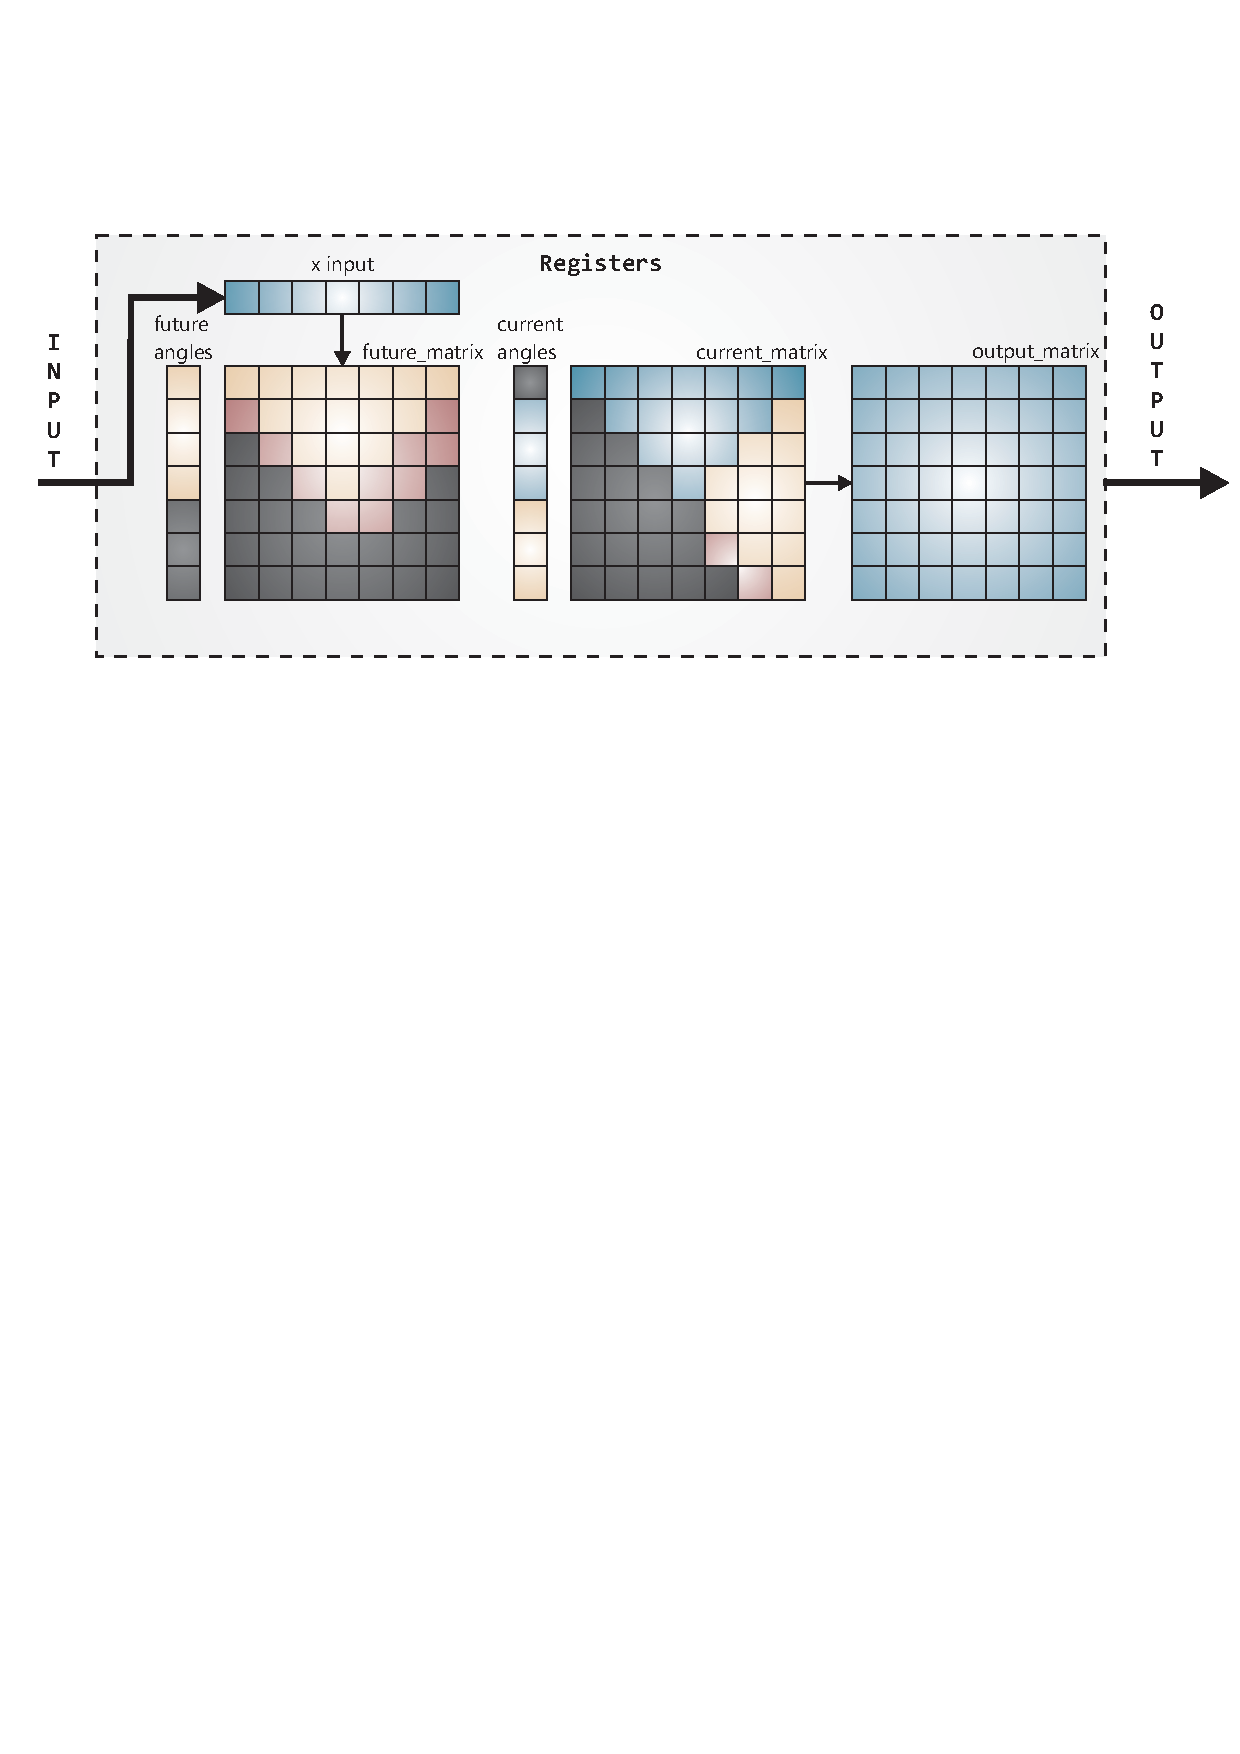
\includegraphics[width=15 cm]{./figures/C04-registers}
 		\caption{Esquema de registros utilizados}
		\label{fig:registers}
 	\end{center}
\end{figure}

Una de las características del mapeo de Walke, es que para lograr la máxima eficiencia de los procesadores, mientras algunos de ellos están procesando el ciclo actual, otros están procesando datos para el ciclo futuro. Por lo cual, en un determinado ciclo de procesamiento se deben almacenar los elementos calculados para dos entradas diferentes. Por este motivo existen las unidades de registros \verb;current_matrix; y \verb;future_matrix;, las cuales son de tamaño \verb;M x N x WORD_WIDTH;. Respectivamente, los ángulos calculados en las operaciones de \textit{boundary cell} son uno por fila, y son almacenados en los registros \verb;current_angles; y \verb;future_angles;.

Finalmente, el bloque de registros \verb;output_matrix; es utilizado para retener el resultado del cálculo de descomposición de una matriz durante toda la etapa de procesamiento, desde que se coloca en alto la señal de \textit{ready} al final de un ciclo, hasta que ocurre el mismo suceso en el siguiente.

Es importante destacar que la lógica de control y los pasos requeridos para la implementación del algoritmo serán descriptos con mayor detalle, y en este caso sólo se explican brevemente las características de los registros.

Se puede observar en el diagrama de la figura \ref{fig:registers} que los elementos de la matriz poseen diferentes colores. Cada uno de ellos representa una característica del registro. Las mismas se describen a continuación:

\begin{itemize}
	\item[•] \textbf{Color Azul}: El color azul representa un registro que se actualiza una única vez durante todo el procesamiento de una matriz. El primer caso es el del registro \verb;x_input;, donde se almacena el nuevo vector de entrada, el cual, concatenado con la matriz anterior, crea la nueva matriz. Luego se tiene un bloque de forma triangular en la parte superior de \verb;current_matrix;. En el mismo, se realiza una copia de los valores de \verb;future_matrix; para luego tenerlos disponibles en los estados de procesamiento. Esto es realizado en una de las etapas tempranas del algorimo. Este es el mismo caso que se da con la primera mitad de \verb;current_angles;. Finalmente, \verb;output_matrix; permanece constante durante todo el procesamiento con el último cálculo de matriz realizado, y se actualiza en el último estado del algoritmo.
	
	\item[•] \textbf{Color Dorado}: Representa un bloque de registros que forman parte del procesamiento del algoritmo, y cambia continuamente durante el mismo. En ellos, se almacenan cada una de las entradas y salidas modificadas por las \textit{boundary\_cells} e \textit{internal\_cells}. El primer caso se da en la matriz \verb;future_matrix;, donde se empieza a calcular una matriz que será finalizada en el próximo ciclo. Por ejemplo, en el ciclo 1 de procesamiento, se utilizan los registros de las posiciones $(1;1)$ y $(2;1)$ de esta unidad. Por otro lado, se tiene la matriz \verb;current_matrix;, donde se almacena el cálculo de la matriz actual, y se utilizan los valores previamente calculados en el sitio anterior. Para seguir con el ejemplo del ciclo 1, se utilizan los registros de las posiciones $(4;5), (5;5), (2;7), (3;7), (3;6), (4;6)$. Finalmente, se tienen los registros donde se leen y escriben los ángulos calculados.
	
	\item[•] \textbf{Color Rojo}: Además de ser registros con las mismas características que poseen los registros dorados, este color representa un registro utilizado para mantener un valor que es requerido en el próximo procesamiento, que sería perdido al realizar el desplazamiento hacia abajo.
	
	\item[•] \textbf{Color Negro}: Representa un registro que no es utilizado. Estos registros se encuentran presentes dado que en Verilog los mismos son creados definiendo los bloques en forma de arreglos bidimensionales. Se verá que, como posibles mejoras, se puede lograr unificar la matriz de salida con estos registros en conjunto con otros adicionales.
\end{itemize}

\subsection{Unidad de control}

A continuación se describirá la unidad codificada para el control del procesador de descomposición QR. La misma fue codificada como una máquina de estados finita. Dado que los estados son consecutivos, la síntesis resulta en un contador, pero la descripción como máquina de estados permite, además de una lectura y entendimiento del código más amigable, el escalamiento del mismo en el futuro. A continuación se describen cada uno de los estados:

\begin{itemize}
	\item[•] \textbf{wait\_vector}: Se trata del estado \textit{idle} del procesador en el que se encuentra a la espera de un nuevo vector, el cual es detectado a través de la señal \verb;start; en alto. El vector que es suministrado desde las entradas del procesador es almacenado en el bloque de registros \verb;future_matrix; en la fila 0. Esto representa una diferencia con el diagrama de registros visto, en el cual se observa un registro separado denominado \verb;x_input;. Se debe tener presente que la fila 0 \textbf{no} es una fila válida de matriz, dado que tanto filas como columnas comienzan desde el subíndice $1$. El registro 0, presente en todos los casos, es agregado como un auxiliar que en este caso es utilizado para almacenar una nueva entrada.
		
	\begin{figure}[h!]
	 	\begin{center}
	 		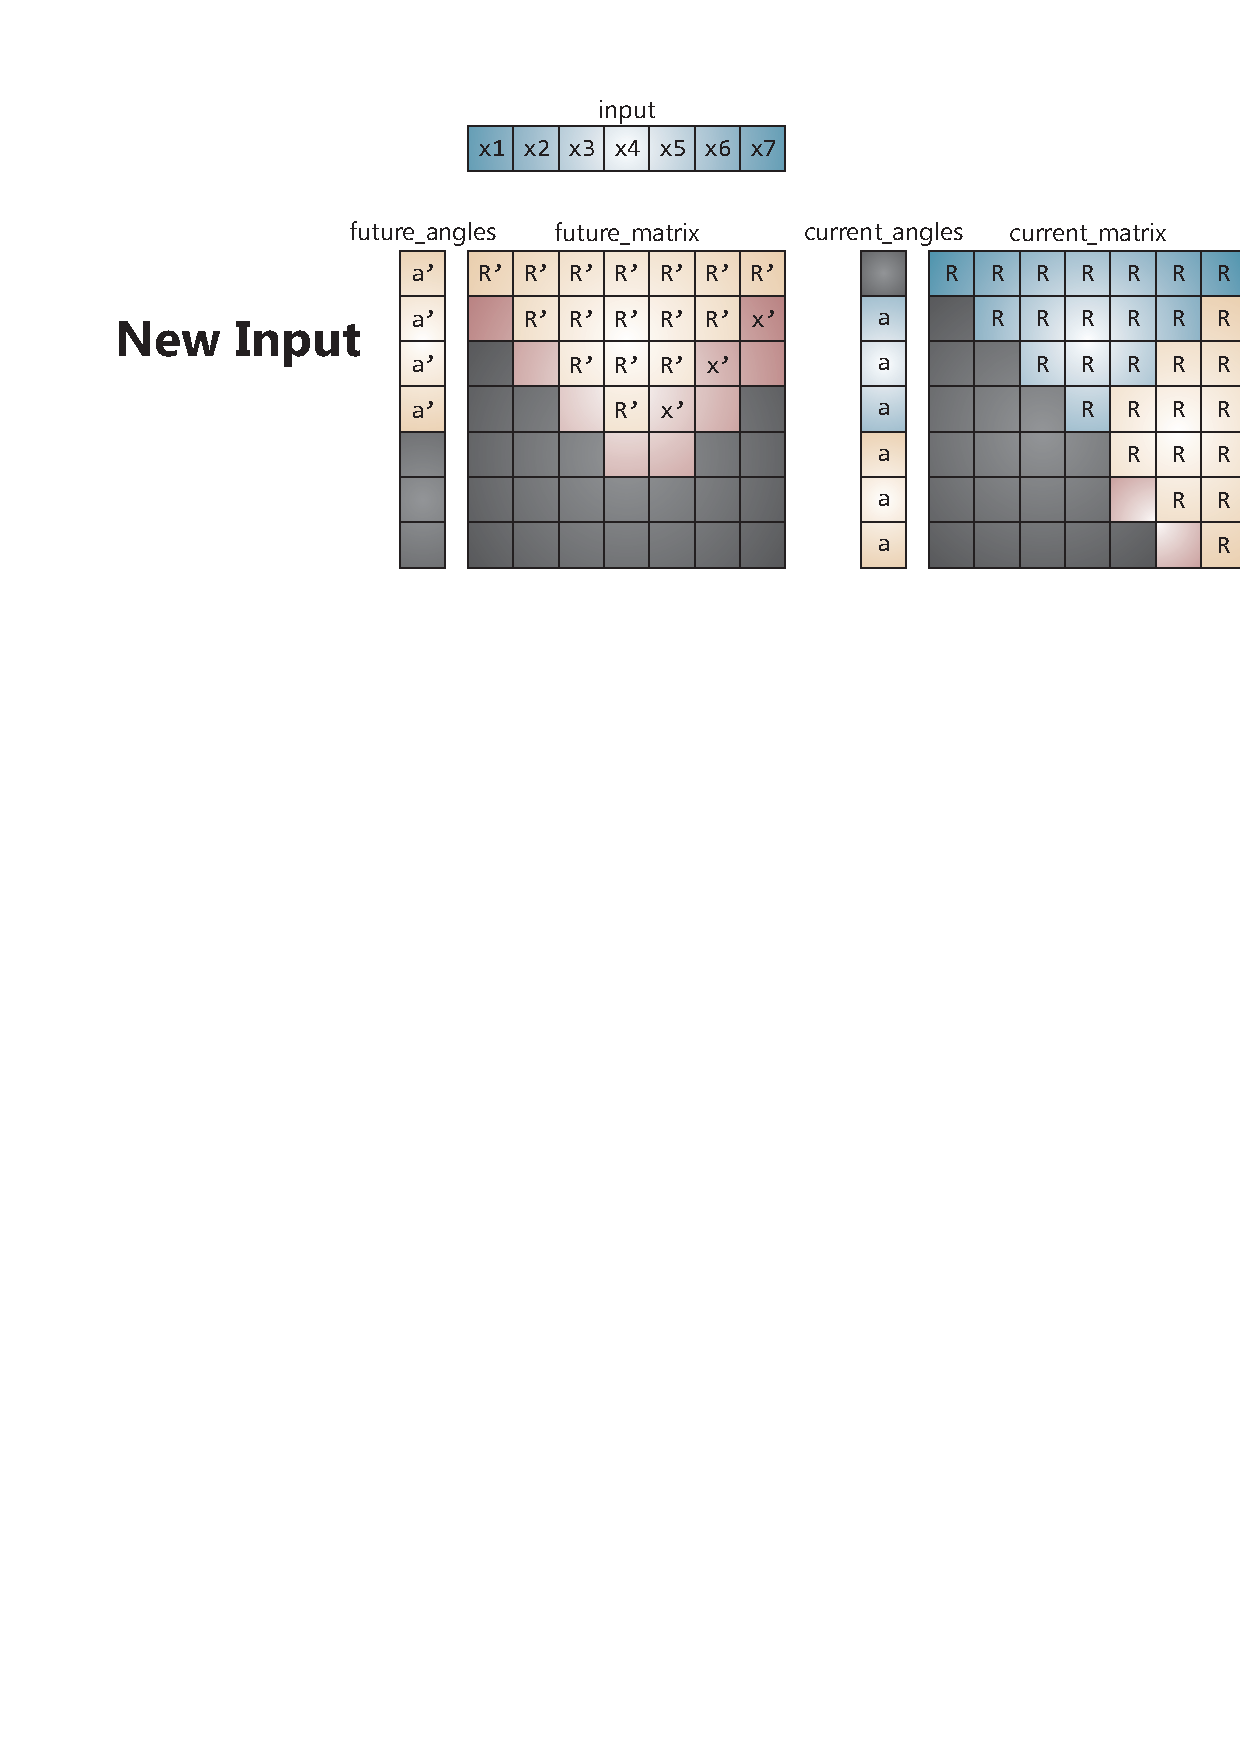
\includegraphics[width=12 cm]{./figures/C04-algorithm_new_input}
	 		\caption{Detección de nueva entrada y estado inicial}
			\label{fig:algorithm_new_input}
	 	\end{center}
	\end{figure}
	
	\item[•] \textbf{shift\_down}: En este estado, con excepción del bloque de registros de salida, se desplazan todos los registros hacia abajo. En \verb;future_matrix;, dado que en la posición $0$ se tiene el nuevo vector $x$, la nueva fila ingresa a la matriz en la fila $1$, se desplazan hacia abajo las demás, y se pierde la última. Los otros registros, con excepción de \verb;output_matrix;, donde no es necesario, también son desplazados hacia abajo para alinearse con el cambio originado por la nueva entrada.
	
	\begin{figure}[h!]
	 	\begin{center}
	 		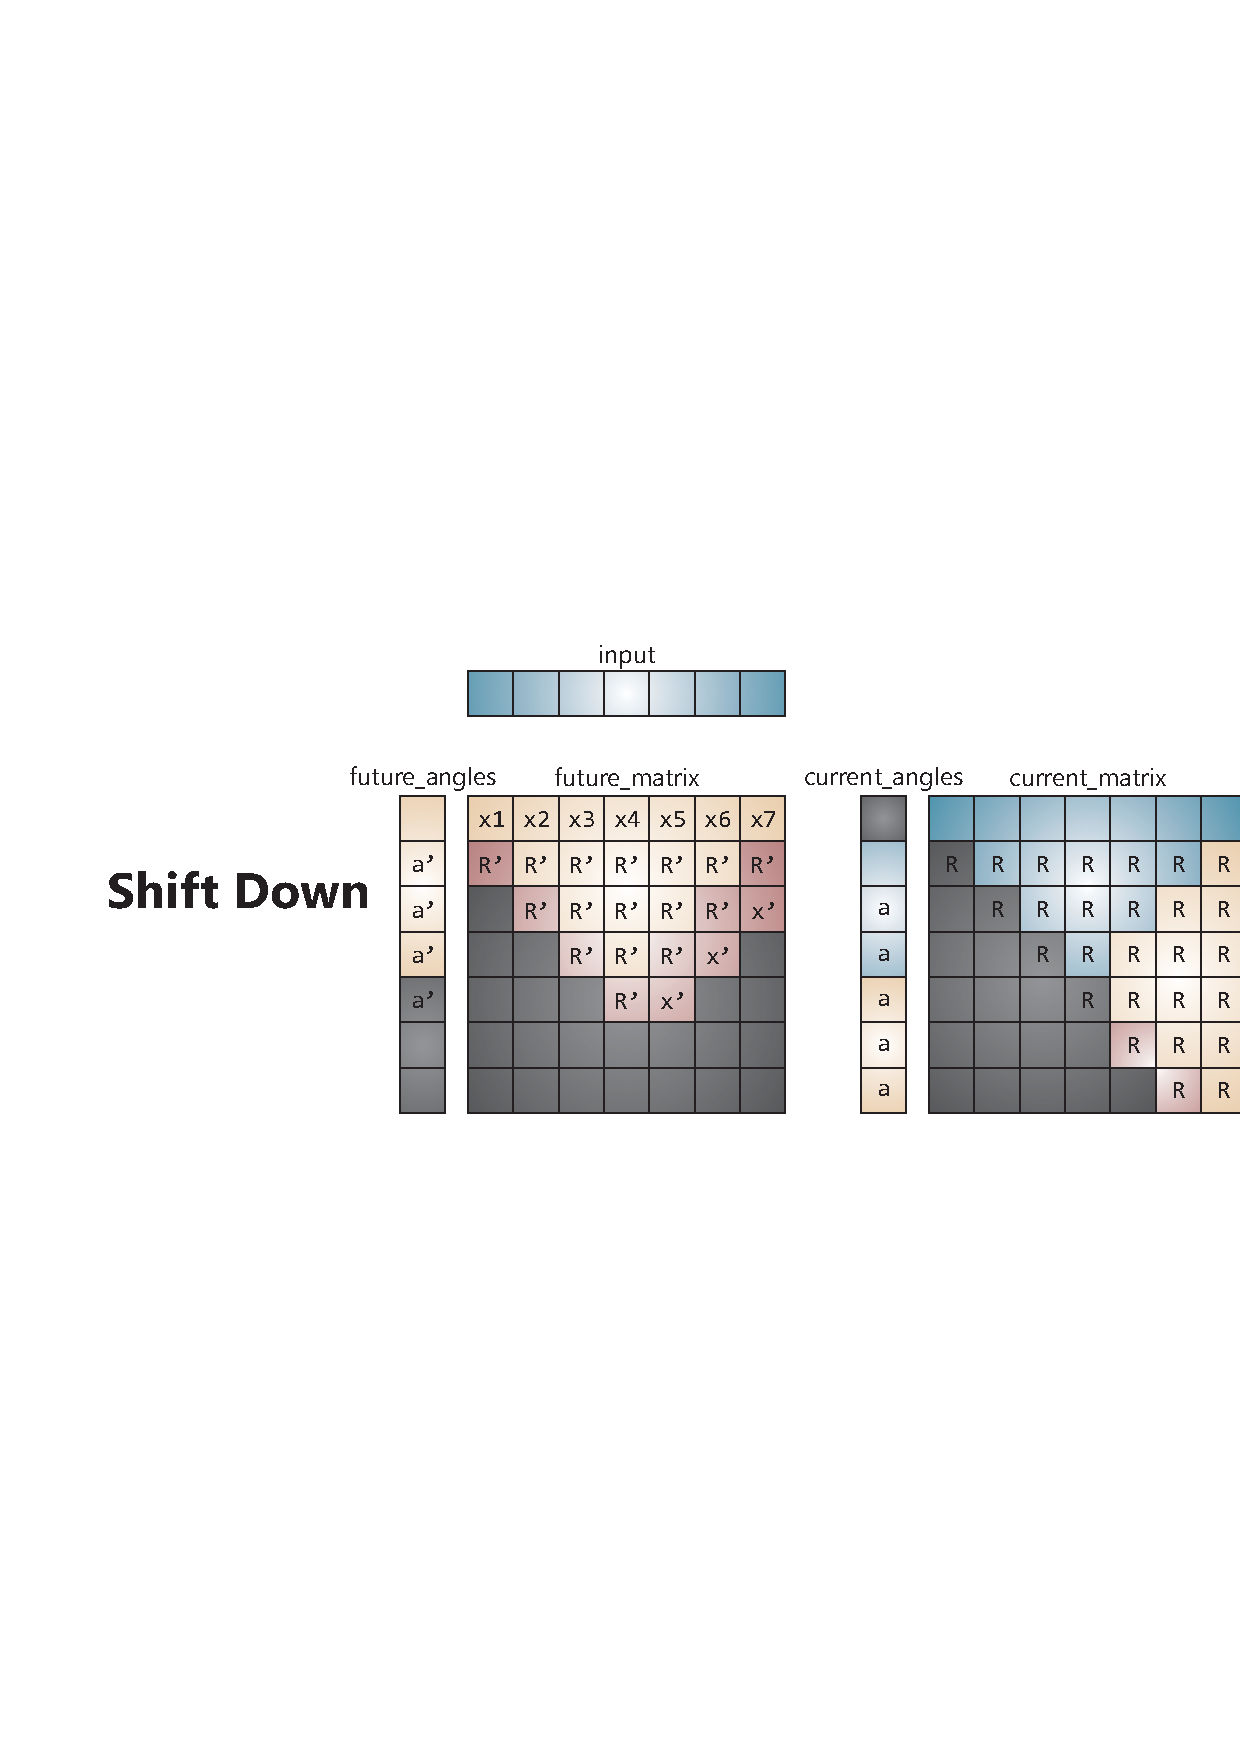
\includegraphics[width=12 cm]{./figures/C04-algorithm_shift_down}
	 		\caption{Resultado del desplazamiento hacia abajo}
			\label{fig:algorithm_shift_down}
	 	\end{center}
	\end{figure}

	\newpage
	
	\item[•] \textbf{copy\_matrix}: Una vez realizado el desplazamiento, se debe realizar una copia de los valores actuales en \verb;future_matrix; a la matriz \verb;current_matrix;. Dichos valores son aquellos que fueron calculados en el procesamiento anterior y conforman la primera mitad del cálculo actual. Se copian los valores de $R$ y de $x$. Adicionalmente, en este estado se comprueba si el vector recibido es el primer vector. En dicho caso, no es necesario hacer ningún procesamiento dado que para que el mismo sea válido es requerido que ingresen en los registros por lo menos dos vectores. Si la comprobación es acertada, se vuelve al estado \verb;wait_vector;.
	
	\begin{figure}[h!]
	 	\begin{center}
	 		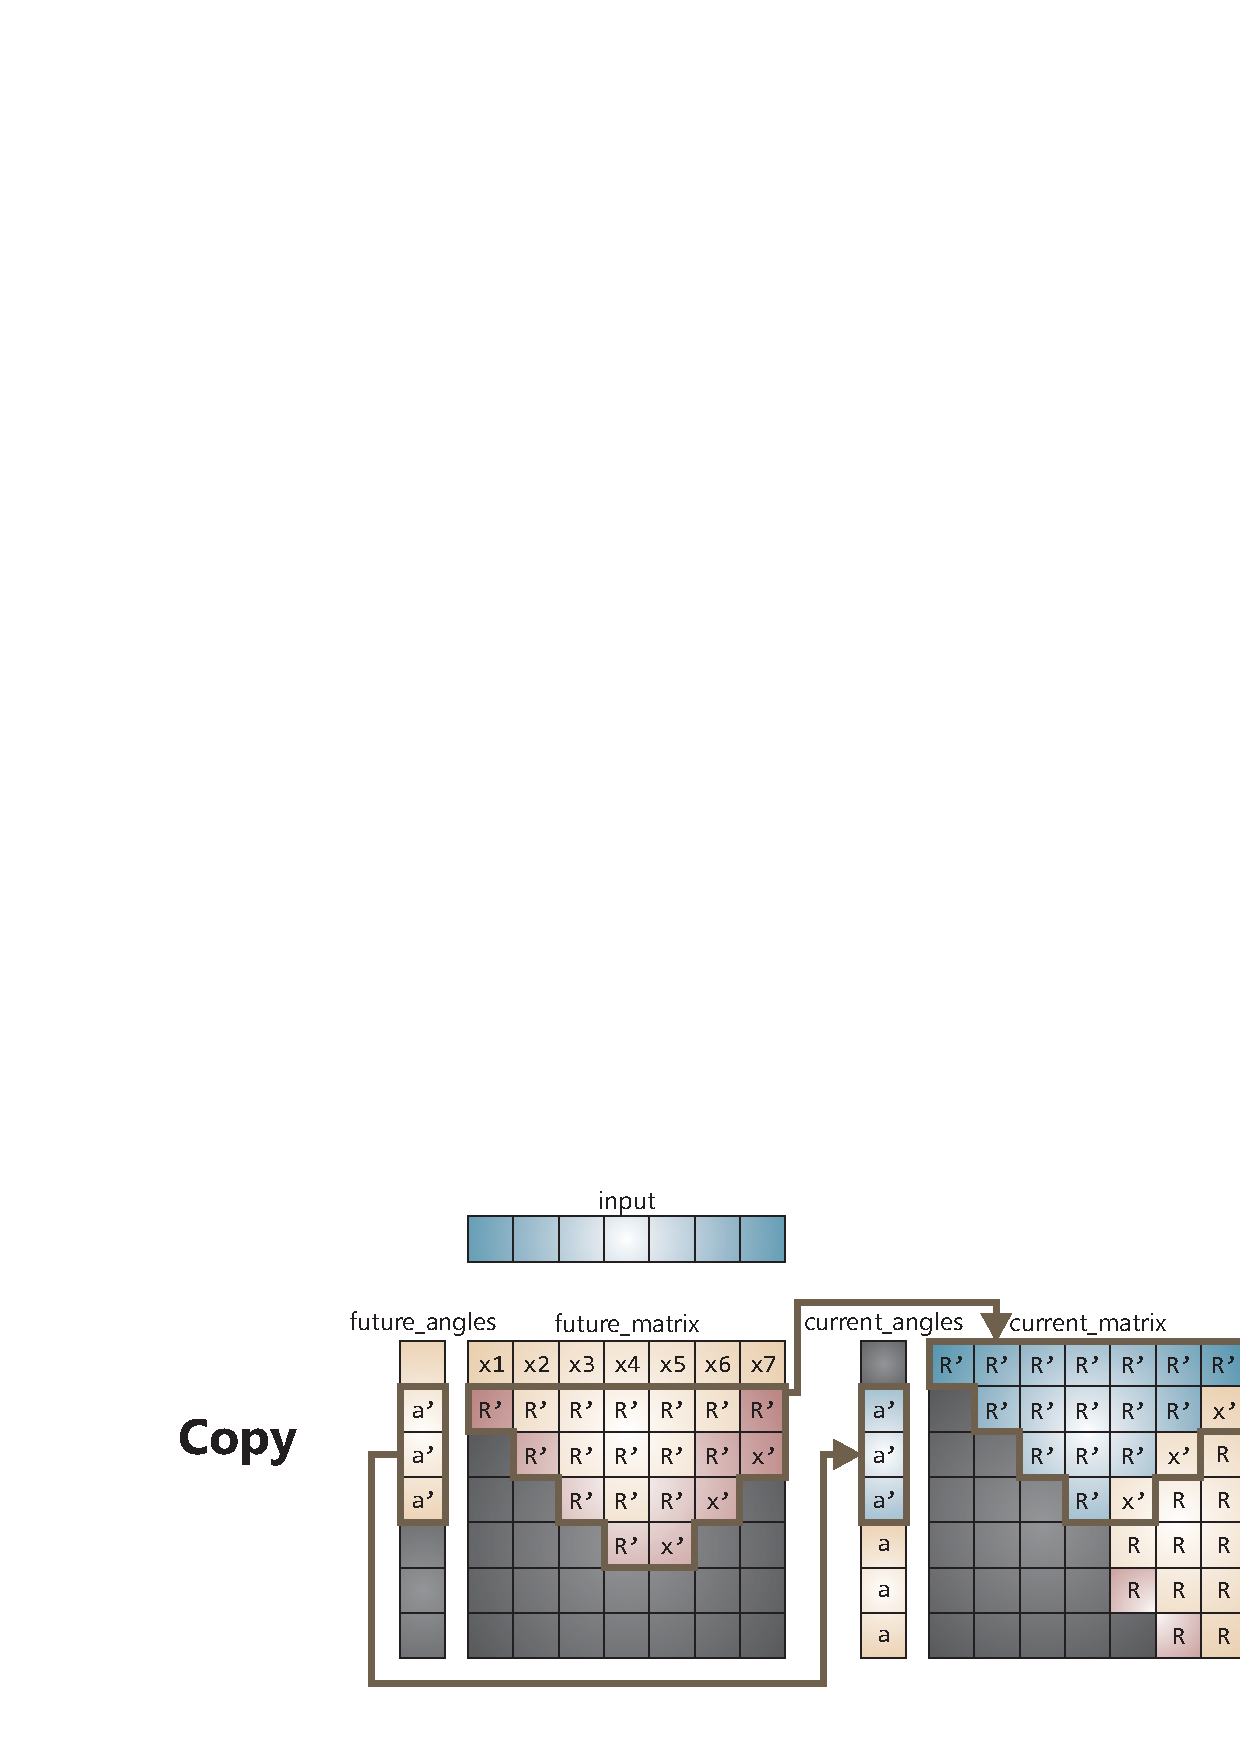
\includegraphics[width=12 cm]{./figures/C04-algorithm_copy}
	 		\caption{Resultado de la copia}
			\label{fig:algorithm_copy}
	 	\end{center}
	\end{figure}

	
	\item[•] \textbf{load\_cycleN} y \textbf{process\_cycleN}: Posterior a la copia, se tiene una serie de estados denominados \verb;load_cycle; y \verb;process_cycle; junto con un número, los cuales consisten en los $N$ estados de procesamiento de los valores $R$ y $x$ de la matriz. En los mismos, se redireccionan las entradas y salidas de las celdas BC e IC, y se controlan las señales de \verb;load; y \verb;ready; para que cada una de las celdas lleve a cabo la rotación correspondiente según las rotaciones de Givens.
	
	Básicamente, el estado \textit{load} consiste en colocar en estado alto la señal \verb;load; suministrando las entradas correspondientes al estado en proceso. Al pasar al siguiente estado, denominado \textit{process}, se pone en estado bajo la señal de \textit{load} y se espera a que todas las celdas coloquen en alto la señal de ready. Una vez detectado dicho suceso, las salidas de las celdas son almacenadas en los registros y el proceso se repite en la siguiente iteración.
	
	\item[•] \textbf{output\_results}: En este estado, se realiza una copia de la imagen actual del bloque de registros \verb;current_matrix; al bloque \verb;output_matrix;. Dado que la unidad \verb;current_matrix; es constantemente modificada durante los ciclos de procesamientos, es requerido copiarlos si se desea retenerlos. Existe un hardware adicional, activado por la señal \verb;send_output;, que lee los valores de la \verb;ouput_matrix; y los escribe en las señales de salida, uno por ciclo de \textit{clock} del procesador QR.
\end{itemize}

En el siguiente capítulo se describirán todos los resultados obtenidos en las simulaciones y síntesis del hardware implementado.

\section{Herramientas utilizadas}

A continuación se hace una breve reseña de las herramientas utilizadas para la implementación del procesador:

\subsubsection*{Sublime Text 2}
\begin{wrapfigure}{r}{0.22\textwidth}
	\vspace{-15pt}
	\begin{center}
		
\includegraphics[width=0.20\textwidth]{./figures/C04-logo_sublime}
	\end{center}
	\vspace{-15pt}
\end{wrapfigure}
Sublime Text fue el principal editor de texto utilizado para codificar en lenguaje Verilog. El mismo presenta una interfaz gráfica con diferentes características de gran utilidad.

\subsubsection*{Vim}
\begin{wrapfigure}{r}{0.22\textwidth}
	\vspace{-20pt}
	\begin{center}
		
\includegraphics[width=0.15\textwidth]{./figures/C04-logo_vim}
	\end{center}
	\vspace{-20pt}
\end{wrapfigure}
Vim es un editor de texto nativo en entornos de tipo UNIX y fue utilizado en algunos casos en conjunto con Sublime Text 2.

\subsubsection*{ModelSim}
\begin{wrapfigure}{r}{0.22\textwidth}
	\vspace{-15pt}
	\begin{center}
		
\includegraphics[width=0.20\textwidth]{./figures/C04-logo_modelsim}
	\end{center}
	\vspace{-15pt}
\end{wrapfigure}
ModelSim fue la herramienta utilizada para la simulación del hardware descripto en código fuente Verilog, con la cual se generaron los archivos de salida de tipo \textit{wave}.

\subsubsection*{gtkwave}
\begin{wrapfigure}{r}{0.22\textwidth}
	\vspace{-15pt}
	\begin{center}
		
\includegraphics[width=0.20\textwidth]{./figures/C04-logo_gtkwave}
	\end{center}
	\vspace{-15pt}
\end{wrapfigure}
Gtkwave fue la herramienta utilizada para visualizar los archivos de tipo \textit{wave} que fueron generados por la simulación realizada en ModelSim.

\subsubsection*{Xilinx ISE}
\begin{wrapfigure}{r}{0.22\textwidth}
	\vspace{-15pt}
	\begin{center}
		
\includegraphics[width=0.15\textwidth]{./figures/C04-logo_ise}
	\end{center}
	\vspace{-15pt}
\end{wrapfigure}
ISE Design Suite es la herramienta proporcionada por la compañía Xilinx para crear los archivos de síntesis ``.bit'' a partir de un hardware codificado en un lenguaje HDL. Dichos archivos .bit implementan el hardware en los dispositivos FPGA que Xilinx provee (Spartan y Virtex, entre otros). También fue utilizada para transferir los archivos ``.bit'' al kit de desarrollo FPGA.

\subsubsection*{Bitbucket}
\begin{wrapfigure}{r}{0.22\textwidth}
	\vspace{-15pt}
	\begin{center}
		
\includegraphics[width=0.20\textwidth]{./figures/C04-logo_bitbucket}
	\end{center}
	\vspace{-15pt}
\end{wrapfigure}
Para realizar el desarrollo se utilizó un repositorio hospedado en \href{http://www.bitbucket.org}{http://www.bitbucket.org}, el cual fue utilizado a través de la herramienta de versionado Mercurial. Dicho sistema aportó diversas ventajas, entre las cuales principalmente se encuentran el mantener un registro de todas las modificaciones realizadas entre cada una de las versiones y el poder trabajar en la nube. En caso de algún comportamiento no deseado al hacer un cambio de versión, el mismo podía ser identificado en el registro proporcionado por la herramienta. El poder trabajar en la nube, facilitó el hecho de poder hacer aportes en el desarrollo desde distintos equipos, ya sea por estar en un equipo de la facultad, del hogar o del trabajo.
\chapter{Estudio, simulación y validación del IP core generado}

En el capítulo anterior se explicó la forma en la cual fue implementado el procesador de descomposición QR en hardware. Se hizo hincapié en las principales características de cada uno de los códigos fuente que definen los módulos que lo conforman.

En el presente capítulo, se expondrán las diferentes herramientas diseñadas para poner a prueba el hardware, tanto aquellas que fueron utilizadas durante su desarrollo como aquellas utilizadas una vez finalizado el mismo para la obtención de métricas. Se implementaron diferentes tipos de bancos de pruebas, cada uno de ellos en base a una necesidad diferente.

Por otro lado, se presentarán todos los resultados de cada una de las pruebas, se plantearán diferentes métricas y se harán comparaciones con otras arquitecturas de procesadores mencionadas en capítulos anteriores (ver sección \ref{sec:analisis_de_publicaciones}).

\section{Emulador de hardware en lenguaje C}

Previamente al desarrollo del hardware en lenguaje Verilog, se optó por poner a prueba el mapeo de Walke del algoritmo utilizando el lenguaje C. Dicho programa iba a aportar diversas ventajas para el proyecto:

\begin{itemize}
   \item[•] Comprender la mecánica del algoritmo y del mapeo de Walke \cite{Walke}, teniendo la posibilidad de extraer resultados parciales paso por paso.
   \item[•] Proveer una fuente de referencia para la comparación de resultados.
   \item[•] Posibilitar la expansión del programa para crear un \textit{testbench} que evalúe el hardware sintetizado en un dispositivo FPGA.
   \item[•] Dado que la sintaxis de Verilog está basada en el lenguaje C, la lógica del mapeo podría ser extraída de este código para ser directamente insertada con mínimas correcciones en el código Verilog y evitar potenciales errores en dicho bloque de desarrollo.
\end{itemize}

El costo de desarrollar dicha herramienta sería mínimo en comparación con el desarrollo del hardware, por lo cual, en base a las ventajas que aportaría, se decidió realizarlo. El mismo se encuentra descripto en el código fuente \verb;qr_decomposition.c;.

La estructura del código fue concebida, no para estar optimizada en cuanto a su funcionalidad, sino para que la sintaxis fuera similar a Verilog, y para que las funciones y datos representaran módulos y registros. Como principales diferencias con respecto al hardware, se tiene que las rotaciones fueron implementadas haciendo uso de las funciones trigonométricas de la librería \verb;math.h;, en lugar de utilizar el algoritmo CORDIC. Asimismo, los datos utilizados fueron de tipo double, con el objeto de trabajar con la máxima precisión disponible.

\begin{figure}[!h]
  \begin{center}
    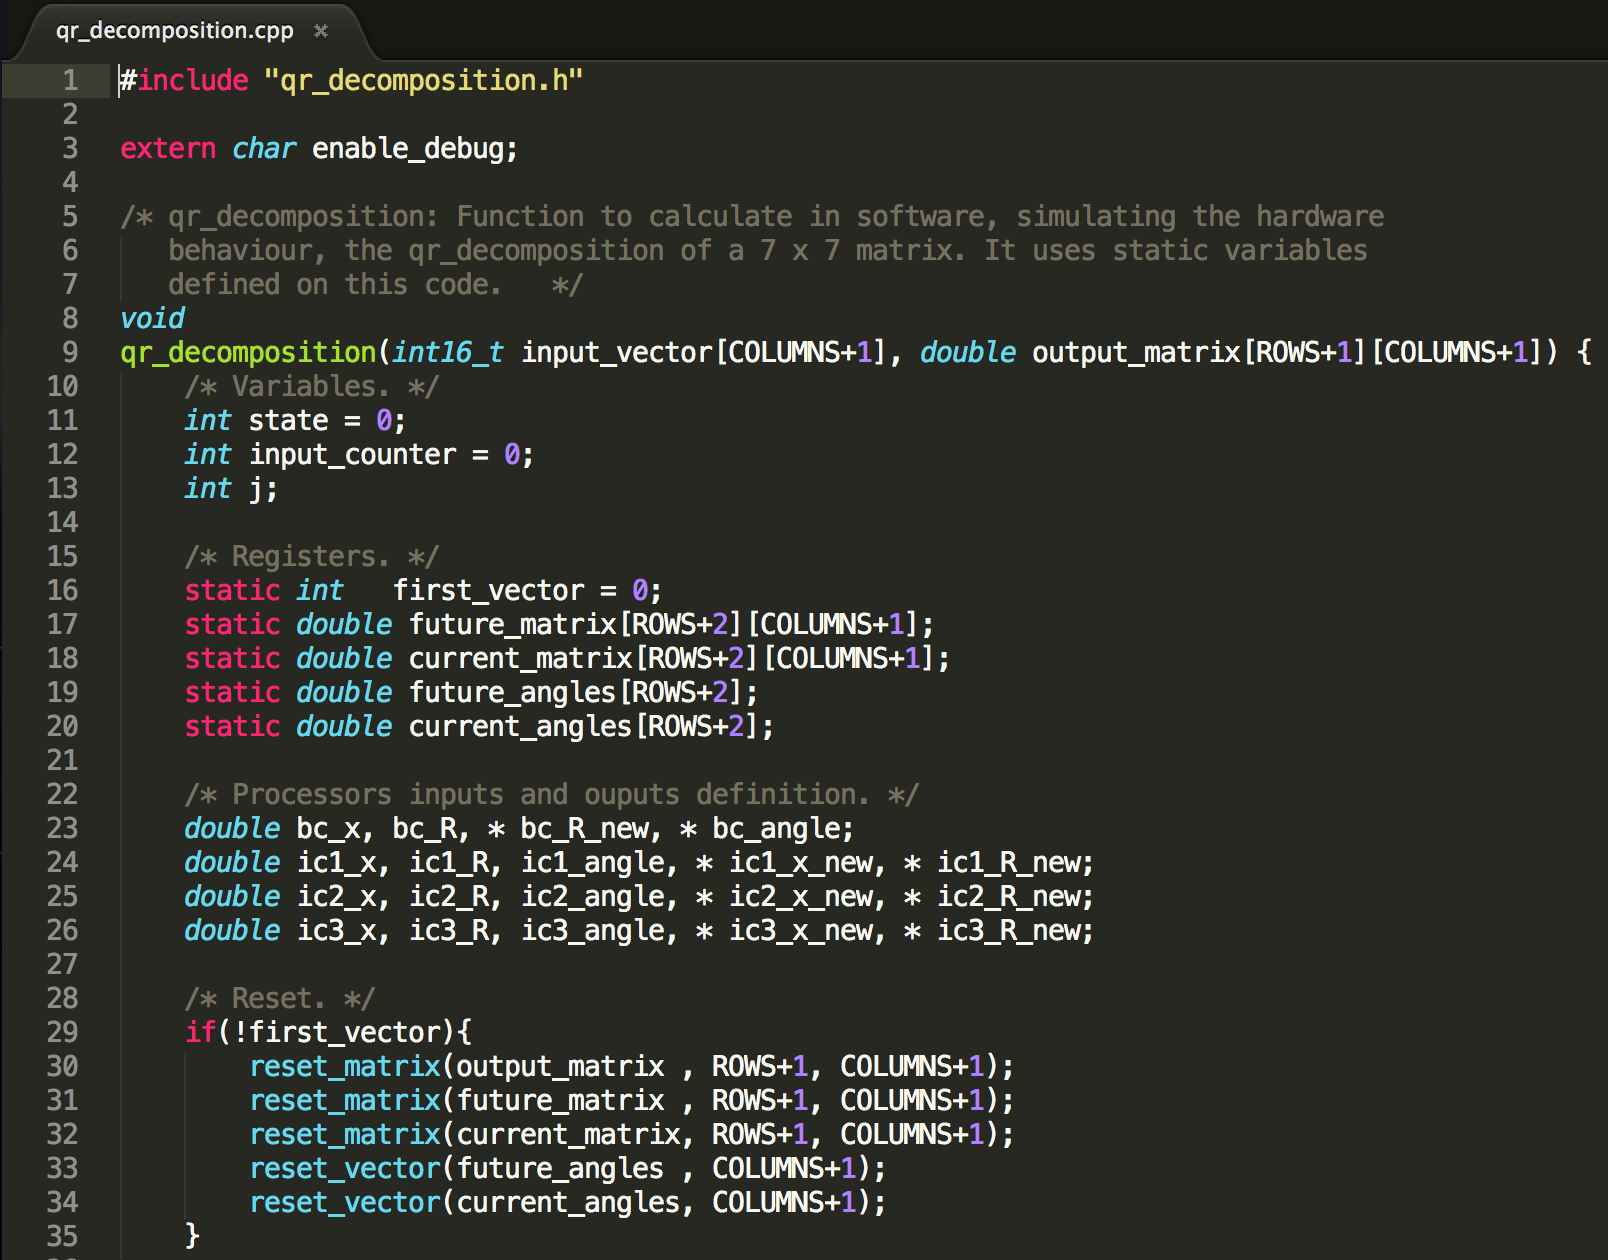
\includegraphics[width=14cm]{./figures/C05-qr_decomposition_code}
    \caption{Extracto de la función de emulación \textit{QR Decomposition}}
    \label{fig:qr_decomposition_code}
  \end{center}
\end{figure}

Con el objeto de validar los resultados de la implementación, se efectuaron pruebas haciendo uso de las herramientas \textit{online} Wolphram Alpha y Bluebit Matrix Calculator. Dichas herramientas poseen motores de cálculo de diferentes funciones matemáticas, entre ellas, la descomposición QR. Se definió una matriz de referencia, la cual fue utilizada en las pruebas realizadas en cada uno de los \textit{testbenchs}:

\begin{figure}[h!]
\[
   \left[
      \begin{array}{ccccccc}
         11012 & 2210  & 2130  & 1140  & 5320  & 6240  & 9870  \\
         8771  & 7722  & 5663  & 4524  & 2695  & 1276  & 1727  \\
         5751  & 18000 & 15578 & 12290 & 15311 & 12260 & 7121  \\
         11110 & 11111 & 13232 & 3245  & 2282  & 13644 & 13373 \\
         13261 & 2223  & 12322 & 9222  & 11115 & 11226 & 12217 \\
         15510 & 11119 & 16553 & 6544  & 6560  & 18861 & 12217 \\
         2571  & 7222  & 11360 & 12650 & 16225 & 12226 & 7912
      \end{array}
   \right]
\]
\caption{Matriz de referencia elegida para las pruebas}
\end{figure}

\begin{figure}[h!]
  \begin{center}
    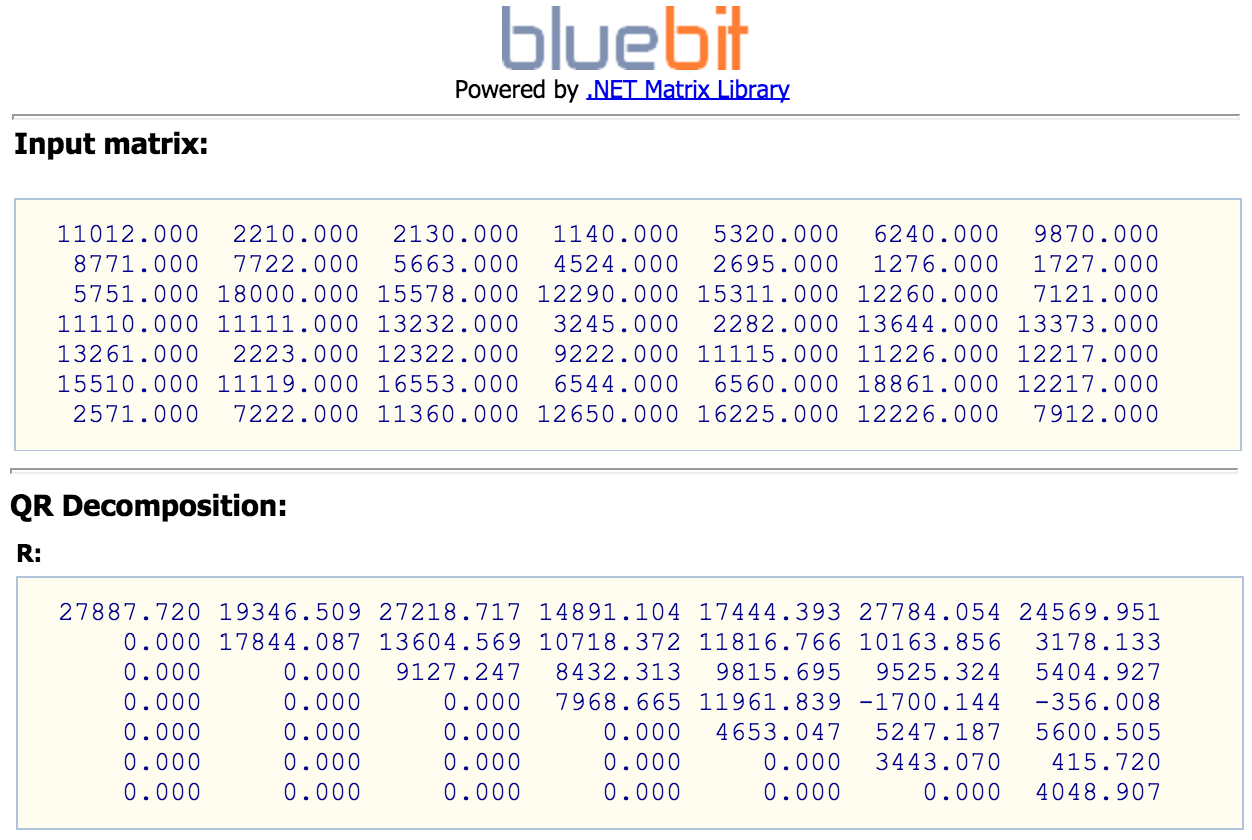
\includegraphics[width=15cm]{./figures/C05-sample_bluebit}
    \caption{Resultado provisto por Bluebit}
    \label{fig:testbench_vs_bluebit1}
  \end{center}
\end{figure}

\newpage

\begin{figure}[h!]
  \begin{center}
    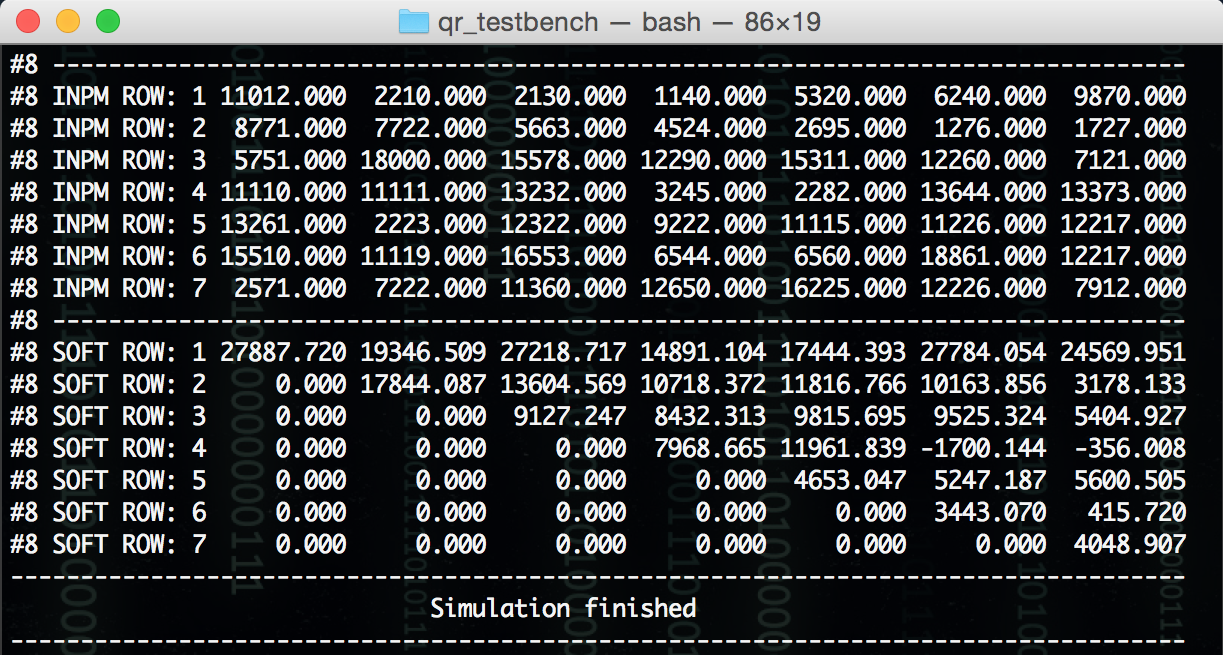
\includegraphics[width=15cm]{./figures/C05-sample_qr_emulator}
    \caption{Resultado provisto por el emulador QR}
    \label{fig:testbench_vs_bluebit2}
  \end{center}
\end{figure}

En las imágenes se puede observar que los resultados del emulador son idénticos a la fuente de referencia utilizada. Al obtener los mismos, se lograron todos los objetivos planteados para este desarrollo.

\newpage

\section{Simulación de módulos en Modelsim}

Como se explicó en capítulos anteriores, al desarrollar un módulo en Verilog se validaba su funcionamiento a través de una simulación utilizando ModelSim. Una vez realizado este proceso con todos los módulos individuales, se procedió a su integración. Luego de una etapa de corrección de diversos errores propios del proceso de desarrollo de hardware, se logró que el mismo entregara el resultado correcto de la descomposición de la matriz de referencia:

\begin{figure}[!h]
 	\begin{center}
 		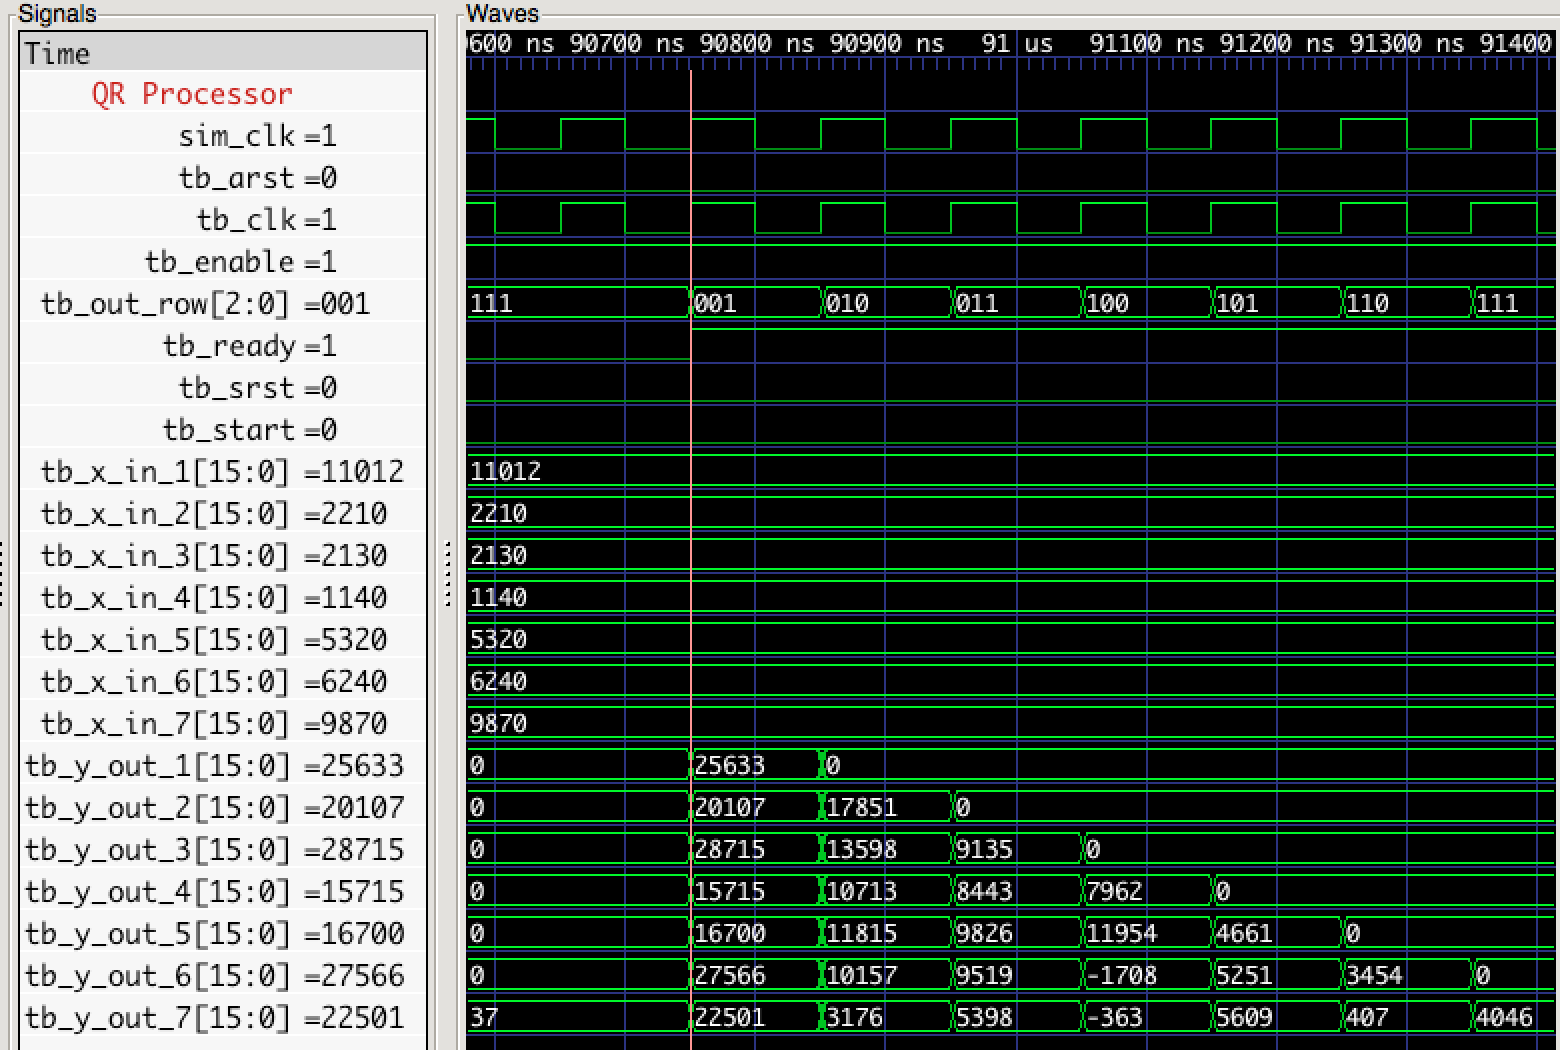
\includegraphics[width=\textwidth]{./figures/C05-sample_qr_processor_wave}
 		\caption{Resultados de la simulación del procesador}
		\label{fig:sample_qr_processor_wave}
 	\end{center}
\end{figure}

En la figura \ref{fig:sample_qr_processor_wave} se puede observar el resultado de las señales de salida del hardware desarrollado, las cuales pueden ser contrastadas contra la función de emulación de la figura \ref{fig:testbench_vs_bluebit2}. Con cierto margen de error, los resultados del emulador desarrollado en lenguaje C y el hardware coinciden. Debido a que la simulación fue realizada utilizando una precisión de 16 bits en punto fijo, la existencia de un margen de error es esperable con respecto a un resultado de 64 bits en punto flotante. En la sección \ref{sec:precision_del_sistema} se hace un análisis de la precisión del procesador.

\section{Interfaz del procesador de descomposición QR}

Una vez validado el funcionamiento del hardware para algunas matrices, se procedió a armar un hardware \textit{top level} para utilizar y comunicar el procesador con otro dispositivo, como por ejemplo una PC. Para ello, se incluyó el procesador de descomposición QR, una unidad UART para realizar la comunicación, y una unidad de control que contenga la lógica necesaria para que el sistema pueda recibir valores, realizar un cálculo y enviar los resultados. Dicho hardware se encuentra descripto en el código \verb;qr_eval.v;. A continuación se presenta un diagrama en bloques del mismo:

\begin{figure}[!h]
  \begin{center}
    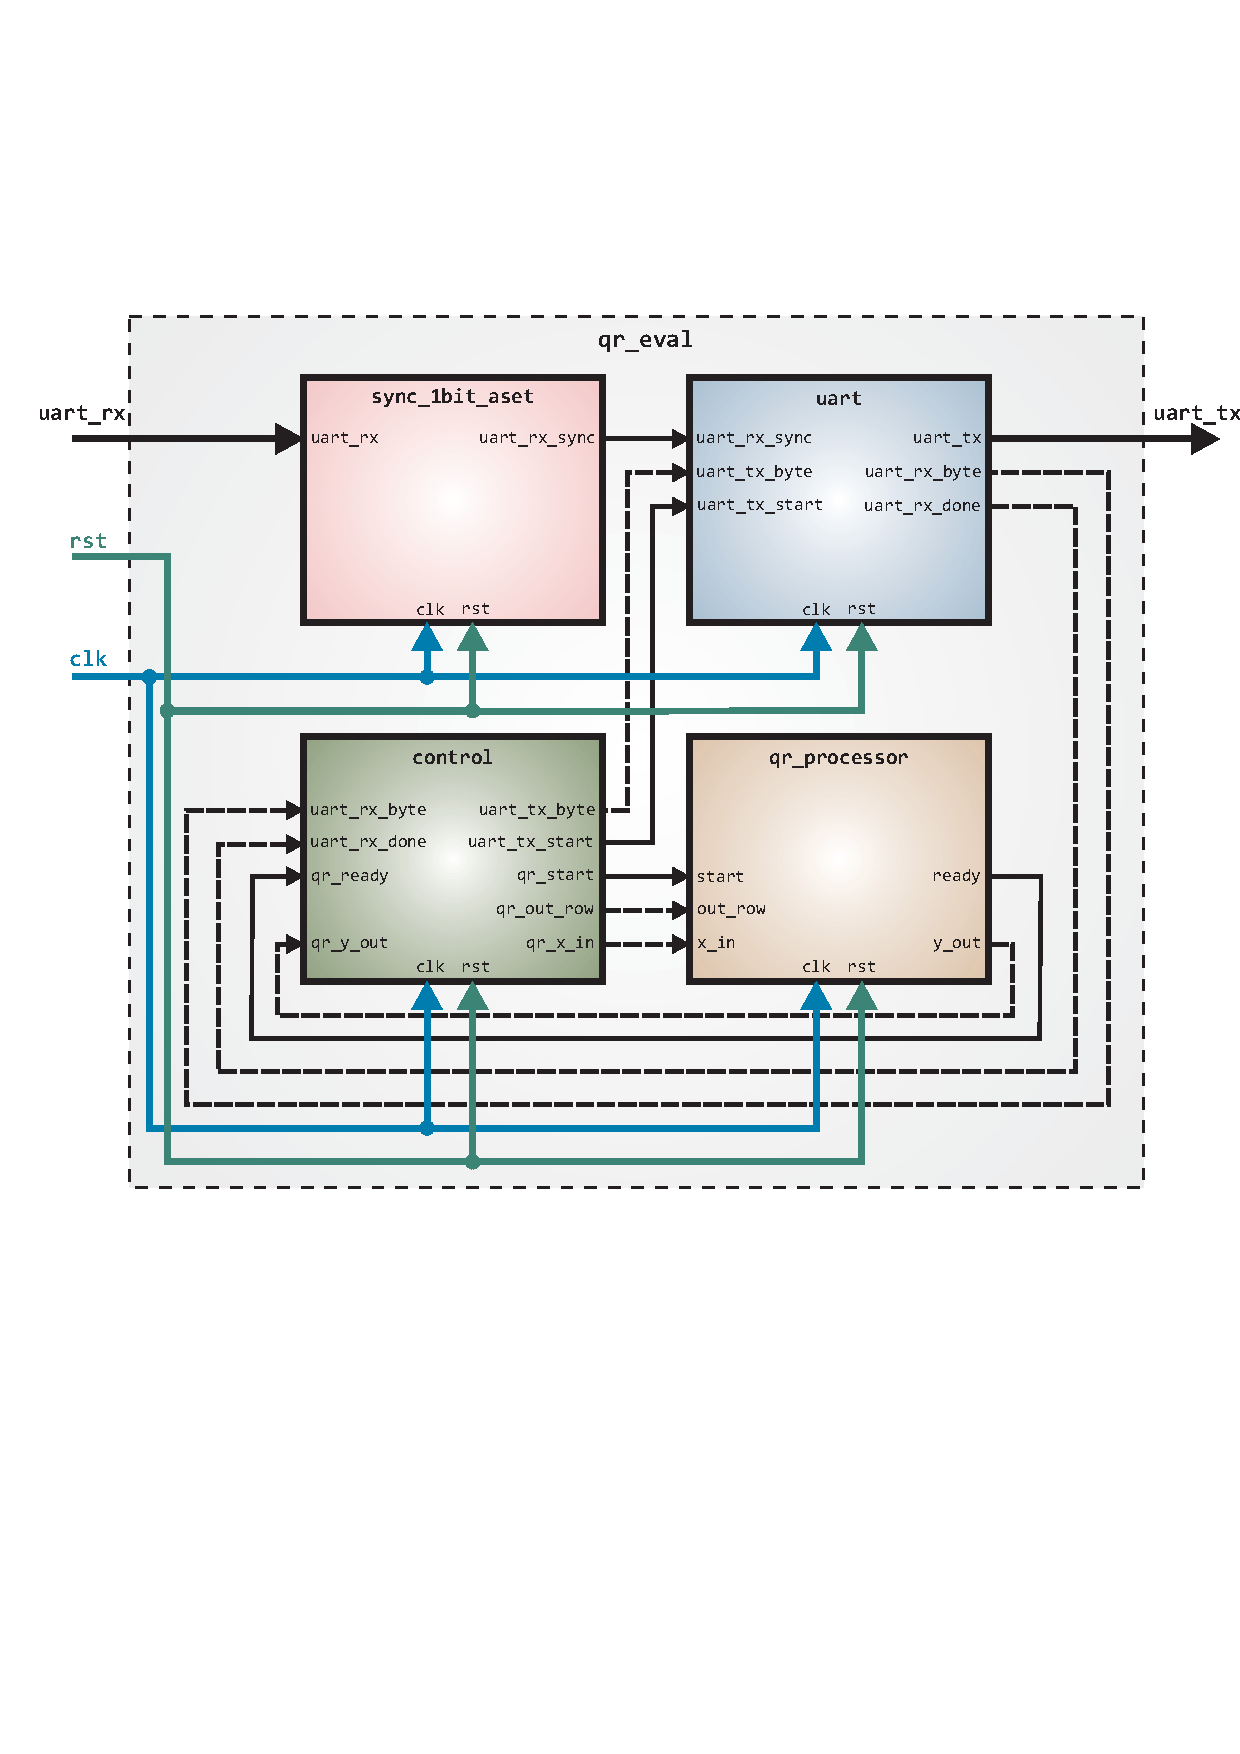
\includegraphics[width=\textwidth]{./figures/C05-qr_eval_diagram}
    \caption{Diagrama en bloques de la interfaz de integración qr\_eval}
    \label{fig:qr_eval_diagram}
  \end{center}
\end{figure}

\newpage

Los estados de la unidad de control siguen el siguiente esquema:

\begin{figure}[!h]
  \begin{center}
    \includegraphics[width=10 cm]{./figures/C05-control_asm}
    \caption{Diagrama en estados simplificado de la unidad de control utilizada en la interfaz}
    \label{fig:control_asm}
  \end{center}
\end{figure}

Una de las características del \textit{top level} es su simplicidad, dado que sólo requiere el conexionado de las líneas de \verb;CLK;, \verb;RST; (para la cual se utiliza un \textit{push button}), \verb;UART RX; y \verb;UART TX; para operar.

\newpage

En la siguiente figura, se observa la simulación del módulo desarrollado, destacando los instantes más importantes de su funcionamiento: 

\begin{figure}[!h]
  \begin{center}
    \includegraphics[width=\textwidth]{./figures/C05-qr_eval_wave}
    \caption{Resultados de la simulación de la interfaz del procesador}
    \label{fig:qr_eval_wave}
  \end{center}
\end{figure}

\section{\textit{Testbench} desarrollado en Verilog}

Teniendo disponible la codificación del hardware completa, se procedió a desarrollar un \textit{script} en lenguaje Verilog para lograr llevar a cabo una prueba intensiva del hardware. Dicho \textit{script} representaría la función que cumple una PC al evaluar el hardware sintetizado, en un entorno de simulación. El mismo debería ser capaz de:

\begin{enumerate}
   \item[•] Tomar 7 líneas de un archivo de entrada para la lectura de vectores de entrada $x$.
   \item[•] Tomar 49 líneas de un archivo de entrada para la lectura del valor esperado de la matriz $R$.
   \item[•] Enviar el vector de entrada utilizado a través de una unidad UART.
   \item[•] Esperar a que el procesador QR realice el cálculo y luego recibir la matriz $R$ a través de la unidad UART.
   \item[•] Presentar los resultados en pantalla en un formato amigable de lectura y escribir los mismos en un archivo de salida simple para su análisis.
\end{enumerate}

Esta lógica se encuentra descripta en el código \verb;qr_host_transactor.v;, el cual es instanciado en la simulación. El \textit{testbench} utiliza 3 archivos diferentes:

\begin{itemize}
   \item \textbf{input\_vector.dat}: Contiene los elementos del vector de entrada separados línea por línea. Luego de 7 líneas, la siguiente representa el primer elemento del siguiente vector.
   \item \textbf{software\_result.dat}: Contiene los elementos de la matriz $R$ calculada en software separados línea por línea. Luego de 7 líneas, la siguiente representa el primer elemento de la siguiente fila. Luego de 49 líneas, la siguiente representa una nueva matriz $R$.
   \item \textbf{hardware\_result.dat}: Se guardan los valores calculados por el hardware utilizando el mismo formato del archivo de software.
\end{itemize}

Los archivos de entrada fueron generados utilizando un programa escrito en lenguaje C denominado \verb;qr_testbench.c;, el cual se explica en la sección \ref{sec:testbench_en_lenguaje_c}. A continuación se expone un ejemplo de un archivo de \textit{input vectors} en el cual se observan los elementos de las primeras 3 filas ingresadas:

\begin{lstlisting}[style=C]
2571
7222
11360
12650
16225
12226
7912
15510
11119
16553
6544
6560
18861
12217
13261
2223
12322
9222
11115
11226
12217
\end{lstlisting}

\newpage

Durante la ejecución del \textit{script} en Verilog, se observa la siguiente salida en pantalla:

\begin{figure}[!h]
  \begin{center}
    \includegraphics[width=11 cm]{./figures/C05-qr_eval_terminal_1}
    \caption{Ejecución de una simulación del cálculo de una matriz en el procesador}
    \label{fig:qr_eval_terminal_1}
  \end{center}
\end{figure}

Se diseñó la interfaz de salida con dos propósitos. En primer lugar se deseaba que rápidamente se pudiera observar de forma organizada cada uno de los elementos de la matriz, siendo posible identificar a qué salida pertenecían. Por el otro lado, se deseaba que la salida pudiera ser procesada a través de expresiones regulares simples con el objetivo de buscar algún resultado en particular. En la misma, es posible identificar los siguientes elementos:

\newpage

\begin{itemize}
  \item[•] \verb;N:; El número al inicio de cada línea representa el número de iteración en el cual se obtuvieron los resultados en dicha línea.
  \item[•] \verb;INPUTVEC:; Representa el \textit{input vector} que se está ingresando en la iteración actual.
  \item[•] \verb;INPM ROW:; Representa las filas de la matriz formada con los últimos 7 \textit{input vectors} ingresados.
  \item[•] \verb;SOFT ROW:; Representa las filas de la matriz $R$ que se obtienen como resultado del emulador en software. Los elementos fueron pre-cargados a través del archivo \verb;software_result.dat;.
  \item[•] \verb;HARD ROW:; Representa las filas de la matriz $R$ que es calculada por el procesador QR simulado. Los elementos son almacenados en el archivo \verb;hardware_result.dat;.
\end{itemize}

Una vez finalizada la simulación, se observa la siguiente salida en pantalla:

\begin{figure}[!h]
  \begin{center}
    \includegraphics[width=10 cm]{./figures/C05-qr_eval_terminal_2}
    \caption{Fin de la simulación del cálculo de una matriz en el procesador}
    \label{fig:qr_eval_terminal_2}
  \end{center}
\end{figure}

\newpage

\section{Síntesis de hardware}

Como se mencionó anteriormente, para llevar a cabo la síntesis del hardware desarrollado, se utilizó la herramienta Xilinx ISE Design Suite 14.1. En principio, se configuró el proyecto para trabajar sobre un dispositivo FPGA Spartan 3E, del cual se disponía un kit de desarrollo para programar el archivo de síntesis. Se utilizó el \textit{kit} de desarrollo \href{http://www.xilinx.com/products/boards-and-kits/hw-spar3e-sk-us-g.html}{Spartan3E Starter Kit}. Es importante destacar que Xilinx cuenta con 4 líneas activas de dispositivos FPGA en función de sus prestaciones, y Spartan3E se trata de un dispositivo discontinuado, que actualmente fue reemplazado por Spartan6, y se encuentra en la línea más básica de ellas:

\begin{figure}[!h]
  \begin{center}
    \includegraphics[width=8 cm]{./figures/C05-xilinx_products}
    \caption{Relación de rendimiento y funcionalidades en dispositivos FPGA Xilinx}
    \label{fig:xilinx_products}
  \end{center}
\end{figure}

\begin{figure}[!h]
  \begin{center}
    \includegraphics[width=8 cm]{./figures/C05-spartan3E_starter_kit}
    \caption{Kit de desarrollo de Spartan 3E}
    \label{fig:spartan3E_starter_kit}
  \end{center}
\end{figure}

\newpage

A continuación se presentan algunas de las características principales de los dispositivos FPGA Xilinx \cite{XilinxFPGA}:

\begin{table}[h!]
   \begin{center}
      \scriptsize
      \begin{tabular}{|c|c|c|c|c|c|c|}
         \hline          
                        & \textbf{Spartan-6} & \textbf{Artix-7} & \textbf{Kintex-7} & \textbf{Virtex-7} & \textbf{Kintex} & \textbf{Virtex}\\
                        &                    &                  &                   &                   & \textbf{UltraScale} & \textbf{UltraScale} \\ \hline \hline
         Logic Cells             & 147,443     & 215,360     & 477,760     & 1,954,560   & 1,160,880   & 4,432,680   \\ \hline
         BlockRAM                & 4.8Mb       & 13Mb        & 34Mb        & 68Mb        & 76Mb        & 132.9Mb     \\ \hline
         DSP Slices              & 180         & 740         & 1,920       & 3,600       & 5,520       & 2,880       \\ \hline
         DSP Performance         & 140GMACs    & 930GMACs    & 2,845GMACs  & 5,335GMACs  & 8,180 GMACs & 4,268 GMACs \\ 
         (symmetric FIR)         &             &             &             &             &             &             \\ \hline
         Transceiver Count       & 8           & 16          & 32          & 96          & 64          & 120         \\ \hline
         Transceiver Speed       & 3.2 Gb/s    & 6.6 Gb/s    & 12.5 Gb/s   & 28.05 Gb/s  & 16.3 Gb/s   & 32.75 Gb/s  \\ \hline
         Total Transceiver       & 50 Gb/s     & 211 Gb/s    & 800 Gb/s    & 2,784 Gb/s  & 2,086 Gb/s  & 5,886 Gb/s  \\ 
         Bandwidth (full duplex) &             &             &             &             &             &             \\ \hline
         Memory Interface (DDR3) & 800         & 1,066       & 1,866       & 1,866       & 2,400       & 2,400       \\ \hline
         PCI Express® Interface  & x1 Gen1     & x4 Gen2     & x8 Gen2     & x8 Gen3     & x8 Gen3     & x8 Gen3     \\ \hline
         Analog Mixed Signal     & -           & XADC        & XADC        & XADC        & System      & System      \\ 
         (AMS)/XADC              &             &             &             &             & Monitor     & Monitor     \\ \hline
         Configuration AES       & Yes         & Yes         & Yes         & Yes         & Yes         & Yes         \\ \hline
         I/O Pins                & 576         & 500         & 500         & 1,200       & 832         & 1,456       \\ \hline
         I/O Voltage             & 1.2V – 3.3V & 1.2V – 3.3V & 1.2V – 3.3V & 1.2V – 3.3V & 1.0 – 3.3V  & 1.0 – 3.3V  \\ \hline
      \end{tabular}
      \caption{Tabla comparativa de dispositivos FPGA Xilinx}
      \normalsize
   \end{center}
\end{table}

Posteriormente, se realizó la síntesis en otros modelos de FPGA con el objetivo de tomar métricas, sin ser el archivo de síntesis de salida utilizado sobre dispositivos FPGA reales. A continuación se muestra la interfaz de la herramienta durante el proceso de síntesis y programación del dispositivo FPGA.

\begin{figure}[!h]
  \begin{center}
    \includegraphics[width=10 cm]{./figures/C05-ISE_synthesis}
    \caption{Resultado de la síntesis en la herramienta Xilinx ISE}
    \label{fig:ISE_synthesis}
  \end{center}
\end{figure}

\newpage

\begin{figure}[!h]
  \begin{center}
    \includegraphics[width=9 cm]{./figures/C05-ISE_programming}
    \caption{Proceso de programación del archivo de síntesis en el dispositivo FPGA}
    \label{fig:ISE_programming}
  \end{center}
\end{figure}

\section{\textit{Testbench} en lenguaje C}
\label{sec:testbench_en_lenguaje_c}

La última herramienta desarrollada fue un programa escrito en lenguaje C que pudiese funcionar como un banco de pruebas del hardware sintetizado. El mismo debía poseer las siguientes características:

\begin{itemize}
   \item[•] Generar un dato que representara vectores de entrada aleatorios, o vectores de entrada de ejemplo, definiendo parámetros tales como la norma máxima de cada elemento y número total de iteraciones.
   \item[•] Utilizar la función \verb;qr_decomposition(); desarrollada anteriormente, para tomar su resultado como una fuente de comparación con máxima precisión.
   \item[•] Abrir una comunicación utilizando un puerto serial para enviar al \textit{kit} de desarrollo el vector de entrada, y recibir del mismo el resultado de la matriz $R$.
   \item[•] Crear archivos numéricos para almacenar los resultados y poder hacer una comparación posterior.
   \item[•] Presentar en pantalla de forma amigable los resultados de las matrices computadas.
\end{itemize}

La herramienta se encuentra definida en el código fuente \verb;qr_testbench.c;. La misma utiliza la línea de comandos para definir el comportamiento del \textit{testbench} que se va a realizar. A continuación se muestra un extracto de la ayuda:

\begin{lstlisting}[style=C]
NAME  
    qr_testbench - A testbench software to assess a QR processor hardware.

SYNOPSIS
    qr_testbench [options]
    
DESCRIPTION
    qr_testbench is a program created to assist the development and testing
    of an implementation of a hardware QR processor. It creates a random vector
    and makes use of a function that replicates the hardware's behaviour using
    the C language. 

OPTIONS
    -n, --norm    
        Defines the maximum value of the input vector elements. The default 
        value if ommited is 1000.
    
    -d, --debug
        Prints special output for debugging purposes.

    -i, --iterations
        Specifies the number of matrices that will be computed. The default 
        value if ommited is 10.
    
    -s, --serial
        Indicates that the serial port will be used to gather the information
        of the QR hardware. The development kit with the synthesized hardware
        must be connected for this option to work. 

    -w, --hwfile
        Indicates that an input file will be used to gather the hardware 
        information. This option may be used to compare the information 
        with the results of a simulation.
    
    -r, --random
        By using this option the input vector generated will be random.
    
    -m, --matrix
        Specifies that the input vector will be generated from a predefined 
        input matrix file supplied by argument.

    -f, --factor
        Specifies the forgetting factor that will be used. The default
        value if ommited is 1.
    
    -h, --help
        Shows a short help about how to use this program.

EXAMPLES
   QR decomposition with lambda = 1 of a matrix formed with 10 vectors with
   non-random elements with norm less than 1000, without using hardware
   results:

         qr_testbench
    
   QR decomposition with lambda = 0.95 of a matrix formed with 200 vectors
   with random elements with norm less than 100, without using hardware
   results:

         qr_testbench -n 100 -i 200 -f 0.95 -r
    
   QR decomposition with lambda = 0.90 using a samples input matrix, without
   using hardware results:
   
         qr_testbench -m sample_matrix.txt -f 0.90
   
   QR decomposition with lambda = 0.90 using an input matrix, connecting the
   testbench to the QR processor hardware using serial port tty.usbserial:
   
         qr_testbench -m sample_matrix.txt -f 0.90 -s /dev/tty.usbserial

   QR decomposition with lambda = 0.90 using an input matrix, taking the
   hardware results from a hardware results file:
   
         qr_testbench -m sample_matrix.txt -f 0.90 -w hardware_results.dat
   
AUTHOR
    Written by Federico Damian Camarda.

REPORTING BUGS
    Report bugs to <fededamian@gmail.com>
\end{lstlisting}

Durante el proceso de síntesis se detectaron errores que no habían sido evidenciados en la etapa de simulación. Luego de la corrección de los mismos se logró el comportamiento adecuado. A continuación se expone una imagen del banco de pruebas en funcionamiento:

\begin{figure}[!h]
  \begin{center}
    \includegraphics[width=\textwidth]{./figures/C05-mac_vs_kit}
    \caption{Testbench: Macbook y el kit de desarrollo con el hardware sintetizado calculando}
    \label{fig:mac_vs_kit}
  \end{center}
\end{figure}

Finalmente, con todas las herramientas descriptas fue posible realizar las diferentes pruebas requeridas para someter el hardware a un continuo proceso de correcciones, evaluar su comportamiento y desempeño, tomar métricas y compararlo con los trabajos analizados. 

\section{Correcciones sobre el hardware implementado}

Al poner a prueba el hardware implementado, se verificó que los resultados obtenidos eran correctos para un número reducido de iteraciones. Sin embargo, al aumentar dicho número, se evidenciaba que los elementos de la matriz comenzaban a incrementarse, hasta finalmente llegar a una condición de \textit{overflow}\footnote{\label{overflow}\textit{Overflow}: Condición en la cual el resultado de una operación de punto fijo produce más bits que sus operandos, en la cual los mismos exceden la longitud de palabra utilizada, lo que resulta en pérdida de información.}. Esto es claramente una condición no deseada, dado que desde el momento en que los cálculos alcanzan la condición de \textit{overflow}, todos los resultados obtenidos comienzan a ser erróneos.

Se estudió este fenómeno desde un punto de vista teórico. Luego de dedicar una gran cantidad de tiempo a analizar el problema, dado que el mismo resultó dificultoso, se detectó que el conflicto en el hardware desarrollado radicaba en el hecho de que poseía un factor de olvido del algoritmo $\lambda = 1$. De esta forma, si el número de vectores se incrementa, esto corresponde a descomponer una matriz $R$ con un orden $n$ que aumenta constantemente. Por lo cual, la condición de \textit{overflow} es inevitable. La misma no es propia del hardware, sino que es propia de la definición teórica del algoritmo al utilizar aritmética de precisión finita.

Con el objetivo de obtener una mejor visión de estos resultados, se desarrolló un \textit{script} Octave, en el cual se ponen en práctica todos los conceptos asociados al algoritmo RLS, y al algoritmo QR-RLS. Dicho \textit{script} permitiría observar gráficamente los imprevistos encontrados, y la forma con la cual se podría resolverlos. El objetivo consistió en definir un sistema a través de un vector de pesos $W$, y utilizar tanto RLS como QR-RLS para estimar dicho vector de pesos. El detalle del \textit{script} puede encontrarse en el \autoref{cap:apB}.

\subsection{Algoritmo QR-RLS}

El primer resultado que se deseaba evidenciar era el constante aumento de los elementos de la matriz $R$ cuando se utilizaba un factor de olvido $\lambda = 1$. Se ejecutó la simulación, y a continuación se expone una gráfica del máximo elemento de la matriz $R$ en función del número de iteración:

\newpage

\begin{figure}[!hbt]
  \begin{center}
    \includegraphics[width=12 cm]{./figures/C05-qrd_rls_max_r_value_lambda_1}
    \caption{Máximo valor de la matriz R en función del número de iteración, $\lambda = 1$}
    \label{fig:qrd_rls_max_r_value_lambda_1}
  \end{center}
\end{figure}

En la figura \ref{fig:qrd_rls_max_r_value_lambda_1} se puede ver claramente el carácter creciente de los elementos de la matriz $R$. Al analizar la bibliografía, se verificó que este conflicto puede solucionarse al utilizar un factor de olvido menor a 1. A continuación se exponen los resultados de la misma simulación, utilizando un factor de olvido $\lambda = 0.95$, un valor utilizado en varias de las diferentes referencias consultadas.

\begin{figure}[!hbt]
  \begin{center}
    \includegraphics[width=12 cm]{./figures/C05-qrd_rls_max_r_value_lambda_095}
    \caption{Máximo valor de la matriz R en función del número de iteración, $\lambda = 0.95$}
    \label{fig:qrd_rls_max_r_value_lambda_095}
  \end{center}
\end{figure}

En contraste con la figura \ref{fig:qrd_rls_max_r_value_lambda_1}, se puede observar en la figura \ref{fig:qrd_rls_max_r_value_lambda_095} que el máximo valor de la matriz R se mantiene por debajo del valor 30000. Analizando este resultado, se evidenció que era necesario implementar en el hardware desarrollado el factor de olvido para valores distintos de $1$.

\subsection{Factor de olvido en el procesador de descomposición QR}

Una vez comprobada la necesidad de implementar un factor de olvido en el hardware desarrollado, se puso en práctica el diseño del mismo. Analizando las ecuaciones presentadas en la sección \ref{sec:mapeo_de_gentleman_y_kung}, se puede observar que el cambio necesario consiste en multiplicar a cada valor $R_{i,j}(n-1)$ por el factor de olvido (referenciado como $\beta$ en la ecuación), y luego realizar el procesamiento en las \textit{boundary cells} e \textit{internal cells} de la misma forma que antes con dicho valor.

Para lograr una arquitectura eficiente, se implementó dicho producto a través del uso de desplazamientos y sumas. Cada vez que se realiza un desplazamiento a derecha de los bits de un registro, esto corresponde a dividir el valor por $2$, por lo tanto:

\begin{align}
R >> 1 &= 0,5    \cdot R \\
R >> 2 &= 0,25   \cdot R \\\nonumber
R >> 3 &= 0,125  \cdot R \\\nonumber
R >> 4 &= 0,0625 \cdot R   \nonumber
\end{align}

Luego, teniendo dichos resultados y sumándolos, se podría llegar a un factor de olvido $\lambda$ equivalente a $0,9375$:

\begin{equation}
(R >> 1) + (R >> 2) + (R >> 3) + (R >> 4) = \\
\end{equation}
\[
0.5 \cdot R + 0.25 \cdot R + 0.125 \cdot R + 0.0625 \cdot R =
\]
\[
0.9375 \cdot R
\]

Lo cual corresponde a un factor de olvido que podría ser utilizado para procesos no estacionarios. Utilizando la técnica descripta anteriormente, se incorporó una entrada de dos bits en el hardware desarrollado que brinda la posibilidad de elegir como factor de olvido los valores $1$, $0,9375$, $0,875$ y $0,75$. Una vez realizada esta corrección, se llegó a la implementación final de hardware de descomposición QR.

\newpage

\section{Resultados}

En la presente sección se detallan los resultados obtenidos durante el ensayo del procesador implementado.

\subsection{Integración del hardware con Octave para la estimación de un sistema}

El \textit{script} desarrollado en la plataforma Octave se divide en cuatro etapas. La primera consiste en la inicialización del sistema. En la misma, se borra la memoria y se crean las señales que se utilizarán en las distintas implementaciones del algoritmo RLS. La señal de entrada $u(n)$ se genera utilizando una distribución normal, y posteriormente es normalizada dividiéndola por el máximo valor del arreglo. El sistema es definido a través del vector de pesos $W$, el cual posee seis elementos definidos de forma arbitraria. El uso de seis elementos es en concordancia con el hardware desarrollado, el cual descompone matrices de dimensión $7 \times 7$ (seis elementos corresponden a los pesos y un elemento a la señal deseada). Luego, a través de la función \verb;filter(); se obtiene la señal deseada $d(n)$. El objetivo del \textit{script} es obtener una estimación del sistema, a través de la definición de un vector de pesos estimado $W_{est}$, de forma tal que su salida, $y(n)$ minimice la función de costo $J(n)$:

\begin{equation}
J(n) = |e(n)|^2 = |d(n) - y(n)|^2
\end{equation}

La segunda etapa del \textit{script} implementa el algoritmo RLS original \cite{Haykin}, sin el uso de descomposición QR. Las ecuaciones se plantean aplicando el lema de inversión de matrices, a partir de las cuales se obtiene el vector de pesos y la señal de salida estimados recursivamente.

La tercer etapa del \textit{script} implementa el algoritmo QR-RLS, de la misma forma que se describe en \cite{Haykin}. Como resultados de esta etapa, no sólo se obtiene el vector de pesos y la señal de salida estimados, sino también la matriz $R$.

Finalmente, en la última etapa del \textit{script}, se pausa el sistema y se solicita el uso del hardware para el cálculo de la matriz $R$ utilizando los vectores de entrada generados. Se realiza este cálculo utilizando las herramientas descriptas previamente (software qr\_testbench conectado via serial al kit de desarrollo), y posteriormente se comparan los resultados. Para obtener el vector de pesos estimado, se aplica una inversión de la matriz $R$ provista por el hardware utilizando una función de Octave.

\newpage

A continuación se exponen los gráficos de resultados:

\begin{figure}[htb!]
    \centering
        \includegraphics[width = 11 cm]{./figures/C05-hard_estimated_output}
        \caption{Señal de salida del sistema original y señal de salida del sistema estimado por el hardware}
        \label{fig:hard_estimated_output}
\end{figure}

\begin{figure}[htb!]
    \centering
        \includegraphics[width = 11 cm]{./figures/C05-hard_error}
        \caption{Señal de error basada en la función de costo utilizando el hardware}
        \label{fig:hard_error}
\end{figure}

\newpage

\begin{figure}[htb!]
    \centering
        \includegraphics[width = 11 cm]{./figures/C05-hard_estimated_weights}
        \caption{Pesos originales vs Pesos estimados utilizando el hardware}
        \label{fig:hard_estimated_weights}
\end{figure}

Como se puede apreciar en los gráficos, los resultados obtenidos a través de la matriz calculada por hardware coinciden con los parámetros definidos en el sistema original con un mínimo margen de error, por lo cual es posible utilizar satisfactoriamente el hardware desarrollado para la estimación del vector de pesos de un sistema.

\subsection{Análisis del error en la estimación de múltiples sistemas}

Una vez comprobado el funcionamiento adecuado para la estimación de un sistema, se procedió a realizar el cálculo para $1000$ sistemas, obteniendo métricas del error. Las métricas tomadas en este caso, para cada sistema estimado, fueron las siguientes:

\begin{equation}
E_1 = \frac{1}{N_w} \sqrt{\sum_{i=1}^{N_w}(W_i-\hat{W}_i)^2}
\end{equation}

donde $N_w$ corresponde al número de elementos del vector de pesos (6 para el presente trabajo), y:

\begin{equation}
E_2 = \text{Max}\{ |W_i - \hat{W}_i| \hspace{0.5cm} \forall \hspace{0.5cm} 1 \leq i \leq N_w\}
\end{equation}

Para ambas métricas, se presenta a continuación el histograma, la media y la varianza que resultan del cálculo de las $1000$ iteraciones.

\newpage

\subsubsection{Métrica $E_1$}

\vspace{-0.5cm}

\begin{figure}[htb!]
    \centering
        \includegraphics[width = 10 cm]{./figures/C05-multiple_system_e1_hist}
        \caption{Histograma de la métrica $E_1$}
        \label{fig:multiple_system_e1_hist}
\end{figure}

\vspace{-0.5cm}

\begin{itemize}
   \item[•] \textbf{Media}: $0.036533$ 
   \item[•] \textbf{Varianza}: $4.1081 \cdot 10^{-4}$
\end{itemize}

\subsubsection{Métrica $E_2$}

\vspace{-0.5cm}

\begin{figure}[htb!]
    \centering
        \includegraphics[width = 10 cm]{./figures/C05-multiple_system_e2_hist}
        \caption{Histograma de la métrica $E_2$}
        \label{fig:multiple_system_e2_hist}
\end{figure}

\vspace{-0.5cm}

\begin{itemize}
   \item[•] \textbf{Media}: $0.15334$ 
   \item[•] \textbf{Varianza}: $6.8030 \cdot 10^{-3}$
\end{itemize}

Se puede observar que, para $1000$ iteraciones, los resultados son consistentes con el análisis realizado para la estimación de un sistema.

\subsection{Precisión del sistema}
\label{sec:precision_del_sistema}

El uso de punto flotante es costoso en términos de hardware, y lleva a diseños que son ineficientes para dispositivos FPGA. La aritmética de punto fijo, utilizada en el presente trabajo, resulta en una implementación en hardware eficiente.

En contrapartida, la aritmética de punto fijo reduce la precisión e introduce dos tipos de errores, de redondeo y de truncamiento. Ambos errores ocurren cuando el resultado requiere más bits que aquella longitud de bits reservada luego de un cálculo. Estos conflictos deben ser manejados cuidadosamente para prevenir \textit{overflow}, lo que desembocaría en resultados incorrectos.

El análisis del error se realiza para todo el procesador de descomposición QR para determinar la relación entre precisión y área. Uno de los mayores problemas al trabajar con aritmética de punto fijo es prevenir el \textit{overflow}.

Para hacerlo, todas las entradas son normalizadas antes de empezar la descomposición. La normalización es realizada dividiendo cada elemento por el más grande, en valor absoluto. De esta forma los elementos estarán siempre entre $-1$ y $1$. Posterior a este proceso, se aplica una constante que asegure que los números se mantengan por debajo del límite numérico del hardware.

El análisis del error es realizado al comparar la aritmética de punto fijo, que resulta del hardware, contra la aritmética de punto flotante de doble precisión, que resulta de la implementación en lenguaje C. El análisis del error es realizada para matrices de 7x7 utilizando precisión de punto fijo de 16 bits.

\subsubsection{Análisis de la condición de \textit{overflow}}

Con el objetivo de obtener una cota para evitar alcanzar la condición de \textit{overflow}, se realizó el siguiente análisis. La matriz $R$ calculada por el hardware resuelve la matriz $\mathbf{\Phi}^{1/2}(n)$. La matriz $\mathbf{\Phi}(n)$ se define a través de la siguiente fórmula:

\begin{equation}
\mathbf{\Phi}(n) = \sum_{i=1}^n \lambda^{n-i} \mathbf{u}(i) \mathbf{u}^H(i)
\end{equation}

Si se plantea un vector $\mathbf{u}(i)$, conformado en todos sus elementos por un único valor considerado máximo, al cual llamaremos $U_{\text{MAX}}$, la matriz toma la siguiente forma:

\begin{equation}
\label{eq:max_phi_1}
\mathbf{\Phi}(n) = \sum_{i=1}^n \lambda^{n-i} U_{\text{MAX}}^2 \mathbf{1} = 
                   U_{\text{MAX}}^2 \mathbf{1} \sum_{i=1}^n \lambda^{n-i}
\end{equation}

donde

\[
\mathbf{1} \text{: Corresponde a la matriz } M \times N \text{ conformada por unos}
\]

Para encontrar el valor máximo que pueden tomar los elementos de la matriz, se debe encontrar el máximo valor que puede alcanzar la serie, la cual será referenciada como $s(n)$. Se analiza la misma observando los primeros tres valores:

\begin{equation}
s(n) = \sum_{i=1}^n \lambda^{n-i}
\end{equation}

\begin{equation*}
   \arraycolsep=1.0pt\def\arraystretch{1.5}
   \left\{
   \begin{array}{lc}
      n = 1 \hspace{1cm} \Longrightarrow \hspace{1cm} & s(n) = \lambda^{1-1} = \lambda^0 \\
      n = 2 \hspace{1cm} \Longrightarrow \hspace{1cm} & s(n) = \lambda^{2-1} + \lambda^{1-1} = \lambda^1 + \lambda^0 \\
      n = 3 \hspace{1cm} \Longrightarrow \hspace{1cm} & s(n) = \lambda^{3-1} + \lambda^{2-1} + \lambda^{1-1} = \lambda^2 + \lambda^1 + \lambda^0
   \end{array} \right.
\end{equation*}

Al analizar los valores que adopta la serie, se observa que se trata de la definición de una serie geométrica, con la diferencia de que los términos aparecen ordenados del mayor al menor. Luego, para una serie geométrica $g(n)$ se tienen los siguientes valores:

\begin{equation}
g(n) = \sum_{i=0}^n \lambda^{n}
\end{equation}

\begin{equation*}
   \arraycolsep=1.0pt\def\arraystretch{1.5}
   \left\{
   \begin{array}{lc}
      n = 0 \hspace{1cm} \Longrightarrow \hspace{1cm} & g(n) = \lambda^0 \\
      n = 1 \hspace{1cm} \Longrightarrow \hspace{1cm} & g(n) = \lambda^0 + \lambda^1 \\
      n = 2 \hspace{1cm} \Longrightarrow \hspace{1cm} & g(n) = \lambda^0 + \lambda^1 + \lambda^2
   \end{array} \right.
\end{equation*}

El máximo valor que puede adoptar la serie, es el valor para la cual converge. Dado que $\lambda$ será un número menor a uno, la serie convergerá a:

\begin{equation}
\label{eq:geo_convergence}
\frac{1}{1-\lambda}
\end{equation}

Aplicando \ref{eq:geo_convergence} a la ecuación \ref{eq:max_phi_1}, se deduce que el máximo valor de la matriz $\mathbf{\Phi}(n)$, el cual llamaremos $\Phi_{\text{MAX}}$, será:

\begin{equation}
\Phi_{\text{MAX}} = U_{\text{MAX}}^2 \frac{1}{1-\lambda}
\end{equation}

Finalmente, dado que la matriz $R$ resuelve la raiz cuadrada, se tiene:

\begin{equation}
\Phi_{\text{MAX}}^{1/2} = U_{\text{MAX}} \sqrt{\frac{1}{1-\lambda}}
\end{equation}

\textit{\textbf{Ejemplo:}} Si se utilizan 16 bits de resolución, y un valor de factor de olvido $\lambda = 0.9375$, el máximo valor que deben poseer los elemenos del vector de entrada se obtiene a partir de la siguiente resolución:

\begin{equation}
2^{16-1} = U_{\text{MAX}} \sqrt{\frac{1}{1-0.9375}}
\end{equation}

\[
32768 = 4 U_{\text{MAX}} \hspace{1cm} \Longrightarrow \hspace{1cm} U_{\text{MAX}} = 8192
\]

\subsubsection{Matrices R}

Si se define al resultado utilizando aritmética de punto flotante de doble precisión como el valor ideal, y al resultado de precisión de punto fijo de 16 bits como el valor estimado, es posible realizar un cálculo del error como sigue.

En primer lugar, se debe caracterizar el resultado de una matriz R a través de un único valor finito. Para ello se calcula el valor promedio de todos los elementos de la matriz R, de la siguiente forma:

\begin{equation}
    R_{double} = \frac{\sum_{i=1}^{7}\sum_{j=1}^{7} R_{i,j}}{7 \cdot 7}
\end{equation}

\begin{equation}
    R_{int} = \frac{\sum_{i=1}^{7}\sum_{j=1}^{7} \hat{R}_{i,j}}{7 \cdot 7}
\end{equation}

Se generan 300 iteraciones de descomposición QR y se grafican a continuación los resultados:

\begin{figure}[h!]
    \centering
        \includegraphics[width = 12 cm]{./figures/C05-precision_1}
        \caption{Salidas ideal y estimada superpuestas}
        \label{fig:precision_1}
\end{figure}

Se puede observar en la figura \ref{fig:precision_1} que las señales de ambos sistemas se encuentran muy cercanas una a la otra, presentando un mínimo margen de error.

\subsubsection{Matriz de error}

Como métrica del error, se toma el valor medio de todos los elementos de la matriz de error, resultante de la diferencia entre la matriz ideal y la matriz estimada, para cada iteración. De esta forma:

\begin{equation}
R_{err} = \frac{\sum_{i=1}^{7}\sum_{j=1}^{7} | R_{i,j} - \hat{R}_{i,j}|}{7 \cdot 7}
\end{equation}

Se generan 300 iteraciones de descomposición QR y se grafican a continuación los resultados:

\begin{figure}[h!]
    \centering
        \includegraphics[width = 12 cm]{./figures/C05-precision_2}
        \caption{Valor medio de la matriz de error}
        \label{fig:precision_2}
\end{figure}

Se puede observar que, en un hardware en el cual la representación numérica se encuentra limitada para números en el rango de $-32768$ a $+32767$, los valores de error oscilan entre -2 y 10. Se presentan a continuación los mismos resultados en términos del valor relativo al mayor número representable, en este caso 32767, y en porcentaje sobre dicho valor:

\begin{figure}[h!]
    \centering
        \includegraphics[width = 12 cm]{./figures/C05-precision_3}
        \caption{Valor medio de la matriz de error relativo al máximo número representable}
        \label{fig:precision_3}
\end{figure}

\begin{figure}[h!]
    \centering
        \includegraphics[width = 12 cm]{./figures/C05-precision_4}
        \caption{Valor medio de la matriz de error en porcentaje}
        \label{fig:precision_4}
\end{figure}

\newpage

\subsection{Parámetros de Timing}

\subsubsection{Máximo clock de operación}

Una vez finalizado el proceso de síntesis, la herramienta Xilinx ISE informa el máximo \textit{clock} con el cual se puede operar el hardware implementado. A partir del valor de este parámetro se deducen los restantes.

\subsubsection{\textit{Throughput}}

Se define al \textit{throughput} como la máxima cantidad de matrices que es posible computar en un segundo. Una vez inicializado el sistema, la cantidad de ciclos de \textit{clock} requeridos para calcular una matriz en cada uno de los estados es la siguiente:

\begin{table}[htb!]
   \begin{center}
      \small
      \begin{tabular}{|c|c|}
         \hline
         \textbf{Estado} & \textbf{Ciclos Requeridos} \\
         \hline
         \hline
         wait\_vector    & 1 ciclo                    \\ \hline
         shift\_down     & 1 ciclo                    \\ \hline
         copy\_matrix    & 1 ciclo                    \\ \hline
         load\_cycle1    & 1 ciclo                    \\ \hline
         process\_cycle1 & \verb;WORD_WIDTH; ciclos   \\ \hline
         load\_cycle2    & 1 ciclo                    \\ \hline
         process\_cycle2 & \verb;WORD_WIDTH; ciclos   \\ \hline
         load\_cycle3    & 1 ciclo                    \\ \hline
         process\_cycle3 & \verb;WORD_WIDTH; ciclos   \\ \hline
         load\_cycle4    & 1 ciclo                    \\ \hline
         process\_cycle4 & \verb;WORD_WIDTH; ciclos   \\ \hline
         load\_cycle5    & 1 ciclo                    \\ \hline
         process\_cycle5 & \verb;WORD_WIDTH; ciclos   \\ \hline
         load\_cycle6    & 1 ciclo                    \\ \hline
         process\_cycle6 & \verb;WORD_WIDTH; ciclos   \\ \hline
         load\_cycle7    & 1 ciclo                    \\ \hline
         process\_cycle7 & \verb;WORD_WIDTH; ciclos   \\ \hline
         output\_results & 1 ciclo                    \\ \hline
      \end{tabular}
      \caption{Ciclos requeridos por cada estado de procesamiento}
      \normalsize
   \end{center}
\end{table}

Por lo tanto, el total de ciclos requeridos responde a la siguiente relación:

\begin{equation}
   \text{Ciclos} = 11 + \text{WORD\_WIDTH} \times 7
   \label{eq:cycles}
\end{equation}

Luego, conociendo la máxima frecuencia de operación, es posible calcular el \textit{throughput} a través de la siguiente fórmula:

\begin{equation}
   \text{\textit{Throughput}} = \frac{f}{11 + \text{WORD\_WIDTH} \times 7}
\end{equation}

\subsubsection{\textit{Update Delay}}

En las publicaciones citadas, se encontró que una de las métricas utilizadas consiste en la cantidad de tiempo que se requiere para procesar una muestra. Se llama a este parámetro \textit{update delay}. Se deduce que este parámetro corresponde a la inversa del \textit{throughput}:

\begin{equation}
   \text{\textit{Update Delay}} = \frac{1}{\text{\textit{Throughput}}}
\end{equation}

\subsubsection{Latencia}

Para analizar la latencia, es necesario calcular la cantidad de segundos requeridos desde que se inicializa el sistema hasta lograr el primer resultado deseado. En el caso del hardware desarrollado, en el proceso de inicialización del sistema, se requiere que se procesen 8 vectores de entrada hasta lograr el primer resultado correcto. Luego, de la ecuación \ref{eq:cycles} que resulta del cálculo de \textit{throughput}, se deduce que la latencia obedece a la siguiente relación:

\begin{equation}
   \text{Latencia} = 8 \cdot \frac{11 + \text{WORD\_WIDTH} \times 7}{f} = \frac{8}{\text{\textit{Throughput}}}
\end{equation}

En la siguiente tabla se exponen los resultados de cada uno de los parámetros presentados anteriormente:

\begin{table}[htb!]
    \begin{center}
      \small
        \begin{tabular}{|c|c|c|c|c|c|}
        \hline  
        \textbf{FPGA} & \textbf{Palabra} & \textbf{Máximo Clock} & \textbf{\textit{Throughput}} & \textbf{\textit{Update delay}} & \textbf{Latencia}\\
        \hline
        \hline
        Virtex 7   & 8 bits  & 133,806 MHz & 1.99710 M & 0.50072 $\mu$s & 4.0058  $\mu$s \\ \hline
        Virtex 7   & 12 bits & 121,522 MHz & 1.27918 M & 0.78175 $\mu$s & 6.2540  $\mu$s \\ \hline
        Virtex 7   & 16 bits & 119,202 MHz & 0.96912 M & 1.03186 $\mu$s & 8.2549  $\mu$s \\ \hline
        Artix 7    & 8 bits  & 104,461 MHz & 1.55912 M & 0.64139 $\mu$s & 5.1311  $\mu$s \\ \hline
        Artix 7    & 12 bits & 89,314 MHz  & 0.94015 M & 1.06366 $\mu$s & 8.5093  $\mu$s \\ \hline
        Artix 7    & 16 bits & 87,563 MHz  & 0.71189 M & 1.40470 $\mu$s & 11.2376 $\mu$s \\ \hline
        Spartan 6  & 8 bits  & 74,425 MHz  & 1.11082 M & 0.90024 $\mu$s & 7.2019  $\mu$s \\ \hline
        Spartan 6  & 12 bits & 71,398 MHz  & 0.75156 M & 1.33057 $\mu$s & 10.6446 $\mu$s \\ \hline
        Spartan 6  & 16 bits & 70,332 MHz  & 0.57180 M & 1.74885 $\mu$s & 13.9908 $\mu$s \\ \hline
        Spartan 3E & 8 bits  & 41,120 MHz  & 0.61373 M & 1.6294  $\mu$s & 13.035  $\mu$s \\ \hline
        Spartan 3E & 12 bits & 39,336 MHz  & 0.41406 M & 2.4151  $\mu$s & 19.321  $\mu$s \\ \hline
        Spartan 3E & 16 bits & 39,503 MHz  & 0.32116 M & 3.1137  $\mu$s & 24.910  $\mu$s \\ \hline
        \end{tabular}
        \caption{Resultados de \textit{timing} para distintos dispositivos FPGA}
      \normalsize
    \end{center}
\end{table}

\newpage

\subsubsection{Resultados en formato gráfico}

\begin{figure}[h!]
    \centering
        \includegraphics[width = 11 cm]{./figures/C05-max_clock}
        \caption{Máximo \textit{clock} de operación para distintos dispositivos FPGA}
        \label{fig:max_clock}
\end{figure}

\begin{figure}[htb!]
    \centering
        \includegraphics[width = 11 cm]{./figures/C05-throughput}
        \caption{\textit{Throughput} para distintos dispositivos FPGA}
        \label{fig:throughput}
\end{figure}

\newpage

\begin{figure}[htb!]
    \centering
        \includegraphics[width = 11 cm]{./figures/C05-delay}
        \caption{\textit{Update delay} para distintos dispositivos FPGA}
        \label{fig:delay}
\end{figure}

\begin{figure}[htb!]
    \centering
        \includegraphics[width = 11 cm]{./figures/C05-latency}
        \caption{Latencia para distintos dispositivos FPGA}
        \label{fig:latency}
\end{figure}

\newpage

\subsubsection{Contraste de resultados de parámetros de timing}

La primera publicación presentada \cite{AlteraQR} corresponde a un procesador sintetizado en dispositivos Altera. Considerando que dicho hardware calcula matrices de $64 \times 9$ y números complejos, es esperable que el rendimiento del mismo sea menor. En este caso, el dato que es posible comparar corresponde al \textit{throughput}. El mejor caso de los tres listados que corresponde al uso de mapeo directo, que corresponde a aproximadamente 0.2 \textit{MSamples} por segundo. El hardware implementado en el presente trabajo puede alcanzar un \textit{throughput} 10 veces mayor, pero cabe aclarar que el mismo calcula  matrices de menor rango ($7 \times 7$) en el dominio de los números reales.

Posteriormente se presentó una publicación de Xilinx \cite{XilinxQR} en la cual se sintetiza un procesador que incluye la dimensión $7 \times 7$ dentro de los resultados. No se especifica el número de bits de ancho de palabra utilizado. El \textit{update delay} presentado para dicho procesador corresponde a $22.62$ $\mu s$, valor que es 22 veces más lento que el valor calculado para el procesador del presente trabajo utilizando 16 bits. El procesador del presente trabajo responde con mayor velocidad, pero es probable que el procesador presentado por Xilinx posea un mayor número de bits de precisión, lo cual explicaría el origen de esta diferencia.

Finalmente, la publicación de la Universidad de Victoria \cite{DongdongQR} expone resultados para un procesador de matrices de dimensión $3 \times 4$, utilizando como mínimo 18 bits. Podemos comparar dichos resultados con el presente procesador para 16 bits. En el caso de la publicación, el procesador presenta un \textit{throughput} de $2,13$ \textit{MSamples / s}, resultado muy similar al del presente trabajo que corresponde a $1,99$ \textit{MSamples / s}. El hardware de la Universidad es ligeramente más rápido, pero menos eficiente, dado que calcula matrices de menor dimensión. Cómo se explicó en la sección \ref{sec:mapeo_de_gentleman_y_kung}, un mapeo directo implica procesadores que no se utilizan el $100\%$ y presentan tiempos ociosos debido a que, para realizar el cálculo, deben esperar a que otros procesadores actualicen la entrada de datos.

\newpage

\subsection{Recursos de FPGA utilizados}

A continuación se presentan los resultados de área de chip obtenidos del reporte de síntesis del hardware desarrollado para 4 tecnologías de dispositivos FPGA Xilinx.

\begin{table}[htb!]
    \begin{center}
      \small
        \begin{tabular}{|c|c|c|c|c|}
        \hline  
        \textbf{FPGA} & \textbf{Ancho de Palabra} & \textbf{LUTs} & \textbf{FFs} & \textbf{Slices} \\
        \hline
        \hline
        Virtex 7      & 8 bits                    & 2257 (1\%)    & 2323         & 636  (1\%)  \\ \hline
        Virtex 7      & 12 bits                   & 2619 (1\%)    & 3076         & 967  (1\%)  \\ \hline
        Virtex 7      & 16 bits                   & 3560 (1\%)    & 4119         & 1306 (1\%)  \\ \hline
        Artix 7       & 8 bits                    & 2218 (1\%)    & 2612         & 1002 (2\%)  \\ \hline
        Artix 7       & 12 bits                   & 2640 (1\%)    & 3172         & 1036 (3\%)  \\ \hline
        Artix 7       & 16 bits                   & 3554 (2\%)    & 4269         & 1783 (5\%)  \\ \hline
        Spartan 6     & 8 bits                    & 2309 (8\%)    & 2647         & 794  (11\%) \\ \hline
        Spartan 6     & 12 bits                   & 2699 (9\%)    & 3184         & 1004 (14\%) \\ \hline
        Spartan 6     & 16 bits                   & 3564 (13\%)   & 4313         & 1329 (19\%) \\ \hline
        Spartan 3E    & 8 bits                    & 3539 (38\%)   & 1211         & 1903 (40\%) \\ \hline
        Spartan 3E    & 12 bits                   & 5299 (56\%)   & 1793         & 2856 (61\%) \\ \hline
        Spartan 3E    & 16 bits                   & 7053 (75\%)   & 2310         & 3813 (81\%) \\ \hline
        \end{tabular}
        \caption{Máximo \textit{clock} de operación}
      \normalsize
    \end{center}
\end{table}

\subsubsection{Resultados en formato gráfico}

\begin{figure}[htb!]
    \centering
        \includegraphics[width = 11 cm]{./figures/C05-luts}
        \caption{Número de \textit{lookup tables} utilizadas}
        \label{fig:luts}
\end{figure}

\newpage

\begin{figure}[htb!]
    \centering
        \includegraphics[width = 11 cm]{./figures/C05-ffs}
        \caption{Número de \textit{flip flops} utilizados}
        \label{fig:ffs}
\end{figure}

\begin{figure}[htb!]
    \centering
        \includegraphics[width = 11 cm]{./figures/C05-slices}
        \caption{Número de \textit{slices} utilizados}
        \label{fig:slices}
\end{figure}

\newpage

\subsubsection{Contraste de resultados de área de chip}

El análisis comparativo de área se realiza únicamente contra la última publicación citada \cite{DongdongQR}, correspondiente a la Universidad de Victoria. Dado que la primera publicación citada corresponde a un hardware desarrollado en dispositivos FPGA Altera, sería difícil hacer una comparación entre sus elementos lógicos ``LEs'' y los elementos lógicos ``LUTs'' de la tecnología Xilinx. Por lo cual en este caso, el análisis es omitido. Por otro lado, la segunda publicación, realizada por Xilinx, no incluye detalles de porcentajes de área de chip utilizados, por lo cual tampoco se considera.

La publicación \cite{DongdongQR} presenta diversas diferencias con la arquitectura desarrollada en el presente trabajo. Al tratarse de arquitecturas diferentes, una comparación directa resulta imposible. En principio, la matriz de la publicación es de menor dimensión ($3 \times 4$), y el mapeo es directo, implicando un mayor número de procesadores. Asimismo, se incluye un bloque de hardware de descomposición adicional utilizado para extraer la matriz $Q$, la cual no se incluye en el hardware del presente trabajo debido a que no es utilizada para la implementación del filtro adaptativo.

Teniendo en cuenta estas consideraciones, se observa que el hardware presentado en \cite{DongdongQR} utiliza un $8\%$ de LUTs y un $11\%$ de \textit{slices} para una implementación de 18 bits de ancho de palabra en un dispositivo FPGA Virtex5. Naturalmente, los porcentajes son mayores a los presentados en el presente trabajo, que se encuentran en el $1\%$ tanto para LUTs como para \textit{slices}, lo cual puede explicarse por el hecho de que el hardware desarrollado posee sólo 4 procesadores, en contraste con los 21 procesadores de la implementación presentada en \cite{DongdongQR}.
\chapter{Conclusiones y trabajos a futuro}

El alcance propuesto para el presente trabajo se basó en los siguientes puntos:

\begin{itemize}
    \item IP Core codificado en el lenguaje Verilog de un procesador de descomposición QR.
    \item Resultado de mediciones pertinentes al diseño del procesador.
    \item Análisis comparativo de procesamiento entre el procesador desarrollado y desarrollos de terceros.
    \item Proposición de trabajos futuros y/o mejoras.
\end{itemize}

Se logró implementar satisfactoriamente un procesador de descomposición QR basado en la arquitectura de Walke\cite{Walke}. Dicha implementación se resume en 14 códigos fuente que contienen la lógica y descripción del hardware en lenguaje Verilog. Adicionalmente, se desarrollaron distintas herramientas que permitieron ensayar el procesador en base a diferentes necesidades.

Como parte del ensayo del procesador, se obtuvieron métricas desde diferentes fuentes. Por un lado, se presentó el resumen de síntesis para cuatro tecnologías FPGA diferentes, utilizando tres valores de longitud de palabra. Dicho resumen permitió conocer el porcentaje de área de ocupación en el chip requerida para implementar el procesador. Este dato es de gran importancia dado que permite entender la cantidad de recursos necesarios para integrar el procesador como un módulo de una implementación mayor, como por ejemplo, un \textit{transceiver} digital.

Se verificó que, en dispositivos FPGA de alta gama, la ocupación se encuentra dentro del 1\%, lo cual permite concluir que el mismo podría ser incluido en un proyecto utilizando dichas tecnologías, sin generar un impacto apreciable en el área de chip. Se obtuvieron parámetros de \textit{timing}, como lo es el máximo \textit{clock} de operación, el cual permite definir la latencia y el \textit{throughput} del hardware. Se obtuvo como resultado que el hardware es capaz de procesar hasta 2 \textit{MSamples} por segundo, el cual es un resultado muy satisfactorio. Por otro lado, se logró identificar la precisión del procesador contrastándolo contra una implementación en software utilizando aritmética de punto flotante de doble precisión, y adicionalmente realizar una estimación de los pesos de un sistema ejemplo mediante el agregado de ecuaciones de sustitución en software. En base a los resultados obtenidos se puede analizar el rendimiento de la implementación y determinar en qué aplicaciones puede ser utilizada.

En base a los resultados de síntesis y de medición, fue posible contrastar la implementación con otras publicaciones similares, con ciertas limitaciones originadas en el hecho de que las arquitecturas y los dispositivos FPGA utilizados son diferentes. Como conclusión general, se puede decir que se implementó una arquitectura capaz de resolver matrices de mayor rango que otras ($7 \times 7$ en contraste con $3 \times 4$) utilizando menor porcentaje de área de chip y velocidad similar, si se toma como referencia la publicación de la Universidad de Victoria \cite{DongdongQR}, la cual presentaba más semejanzas entre las tres analizadas.

Este trabajo presenta una primera implementación de un procesador de descomposición QR, con un gran número de posibilidades para mejorar y optimizar el diseño. Como potenciales trabajos a futuro, en el contexto de la presente tesis, se destacan los siguientes:

\begin{enumerate}
	\item Complementar el hardware desarrollado, que consta únicamente del procesador de descomposición QR, con el hardware de sustitución, con el objetivo de conseguir el hardware requerido para la obtención de los pesos de un filtro adaptativo.
	\item Ensayar el \textit{beamformer} en un ambiente de prueba real, mediante el uso de \textit{front-ends} con antenas y conversores AD.
    \item Modificar el \textit{pipeline} y realizar otro tipo de optimizaciones, con el objeto de lograr mejorar las métricas (aumentar el máximo \textit{clock} utilizable, disminuir la latencia y aumentar el \textit{throughput}, o reducir el área de chip).
	\item Modificar el hardware para operar con números complejos, representando las componentes IQ de la modulación en cuadratura.
	\item Parametrizar el hardware para operar con distintos números de filas y columnas, como por ejemplo, matrices de $N \times N$ igual a $3 \times 3$, $4 \times 4$ o $5 \times 5$. En función del número de columnas, se podrán utilizar 2 antenas + 1 señal deseada, 3 antenas + 1 señal deseada ó 4 antenas + 1 señal deseada, respectivamente.
	\item Modificar el hardware para operar con otros mapeos diferentes al de Walke\cite{Walke}, con mayor número de procesadores para lograr \textit{throughputs} mas altos.
	\item Sintetizar y ensayar el hardware en un dispositivo FPGA \textit{state of the art}, como por ejemplo Virtex7.
	\item Incorporar la posibilidad de cambiar el algoritmo de rotación (algoritmo CORDIC en el hardware implementado) por otros, como ejemplo Gram Schmidt, o SGR (Squared Givens Rotations).
	\item Modificar el hardware para operar con memoria RAM en lugar de una unidad de registros.
\end{enumerate}

% Apéndices
\appendix
\chapter{Código fuente Verilog del procesador QR desarrollado}
\label{cap:apA}

\section{Fuente qr\_processor.v}

\lstinputlisting[language=Verilog]{../../../../projects/hardware/qr_processor/rtl/source/qr_processor.v}

\section{Fuente boudary\_cell.v}

\lstinputlisting[language=Verilog]{../../../../projects/hardware/qr_processor/rtl/source/boundary_cell.v}

\section{Fuente internal\_cell.v}

\lstinputlisting[language=Verilog]{../../../../projects/hardware/qr_processor/rtl/source/internal_cell.v}

\section{Fuente rotator.v}

\lstinputlisting[language=Verilog]{../../../../projects/hardware/qr_processor/rtl/source/rotator.v}

\section{Fuente iterative\_cordic.v}

\lstinputlisting[language=Verilog]{../../../../projects/hardware/qr_processor/rtl/source/iterative_cordic.v}

\section{Fuente preprocessor.v}

\lstinputlisting[language=Verilog]{../../../../projects/hardware/qr_processor/rtl/source/preprocessor.v}

\section{Fuente post\_multiplier.v}

\lstinputlisting[language=Verilog]{../../../../projects/hardware/qr_processor/rtl/source/post_multiplier.v}
\chapter{Script Octave de análisis de resultados}
\label{cap:apB}

\begin{lstlisting}[style=C]
% -----------------------------------------------------------------------------
% Name:          rls_analysis.m
% Version:       1.1
% Author:        Federico Damian Camarda
% Date:          09/04/2015
% Description:   Framework to work with the RLS algorithm.
% References:    [1] S. Haykin, Adaptive Filter Theory. 3rd edition pp. 562.
%                    RLS Algorithm.
%                [2] S. Haykin, Adaptive Filter Theory. 3rd edition pp. 598.
%                    QRD RLS Algorithm.
% -----------------------------------------------------------------------------
%
% Block Diagram:
%
%              _________                  _____
%  u(n) ----> |         | ---> d(n) ---> |+    |
%        |    |    W    |                |     |
%        |    |_________|                | sum |
%        |     _________                 |     | ---> e(n)
%        |    |         |                |     |
%        ---> |  W_est  | ---> y(n) ---> |-    |
%             |_________|                |_____|
%
% The u(n) signal is filtered with the W system to generate the desired signal
% d(n). The W system is manually defined.
%
% The RLS algorithm is used to compute the W_est filter, an estimated system
% that, when filtering u(n) with W_est it outputs a signal y(n) that minimizes
% the cost function J(n) = |e(n)|^2 = |d(n) - y(n)|^2
% -----------------------------------------------------------------------------

% Initialize environment.
clc                            % Clean terminal.
clear all                      % Clear environment.
close all                      % Close windows.
diary('rls_analysis.term')     % File where terminal output will be saved on.
diary on                       % Save terminal output on.

% Control parameters.
enable_plots_rls         = 0;
enable_plots_rls_qr      = 0;
enable_plots_rls_qr_hard = 0;
enable_plots_precision   = 1;
enable_debug             = 0;
enable_hard_file         = 1;

% Samples related signals.
N      = 300;                  % Number of samples.
n      = 1:N;                  % Samples' index.

% Filter related signals.
W      = [2 -1 0 0 -1 2]';     % Unknown System coefficients.
N_w    = length(W);            % Filter weigths length.
n_w    = 1:N_w;                % Filter weigths index.
An     = 5000;                 % Multiplying constant.
u      = randn(1, N);          % Input to the filter.
u      = An * u / max(abs(u)); % Normalized input.

% Observed signal.
d      = filter(W, 1, u);

% -----------------------------------------------------------------------------
%                     1. Standard RLS Algorithm : Equations
% -----------------------------------------------------------------------------

% RLS Algorithm implemented by the equations described in [1].
% Zero padding of N_w values is applied to u(n). The reason is that the input
% of the algorithm requries that the first vector is [ 0 0 ... 0 u(n) ],
% the next [ 0 0 ... u(n) u(n-1) ], and so on until the vector is completed.

lambda = 0.9375;                 % RLS forgetting factor.
v      = 1;                      % Initial input variance estimate.
P      = eye([N_w, N_w]) / v;    % Initial inverse correlation matrix.
W_est  = zeros(N_w, 1);          % Initial weights.
u      = [zeros(1, N_w - 1), u]; % System input u(n) with zero padding.
y      = [ ];                    % Output of the estimated system.
e      = [ ];                    % A posteriori error.
xi     = [ ];                    % A priori error. (xi: from the greek letter)

% Open file descriptor to save input vectors.
fid    = fopen('input_vectors_matlab.txt','wt');

% Start algorithm.
for i=1:N                       % All time steps.
    % Take the last N_w samples from the observation.
    U     = u(i + N_w - n_w)';  % e.g. for i=1, => 6,5,4,3,2,1;
                                %      for i=2, => 7,6,5,4,3,2;

    % Save vector in a file.
    fprintf(fid,'%f ',U);
    fprintf(fid,'%f ',d(i));
    fprintf(fid,'\n');

    % Save the estimated output.
    y(i)  = W_est' * U;
    
    % Filter gain.
    K     = (1 / lambda) * P * U / (1 + (1 / lambda) * U' * P * U);

    % Error signal equation. A priori error.
    xi(i) = d(i) - W_est' * U;

    % Filter coefficients.
    W_est = W_est + K * xi(i);

    % Error signal equation. A posteriori error.
    e(i)  = d(i) - W_est' * U;

    % Inverse correlation matrix update.
    P     = (1 / lambda) * P - (1 / lambda) * K * U' * P;
end

% Close file descriptor.
fclose(fid);

% -----------------------------------------------------------------------------
%                      2. Compute the results with hardware
% -----------------------------------------------------------------------------

% Process hardware results if flag is enable.
if(enable_hard_file)
    % Give time to the operator to process the samlpes.
    disp('Samples are ready to be processed.');
    pause

    % Read the hardware results and store them in hard_matrix_16.
    for i=n
       hard_matrix_16(:,:,i)=dlmread('hardware_result_matlab.dat',' ',
                                     [(i-1)*7 0 (i-1)*7+6 6]);
    end

    % Read the software results and store them in soft_matrix_16.
    for i=n
       soft_matrix_16(:,:,i)=dlmread('software_result_matlab.dat',' ',
                                     [(i-1)*7 0 (i-1)*7+6 6]);
    end

    % Mean value of the matrix
    for i=1:N-1
        hard_matrix_mean_value(i) = sum(sum(hard_matrix_16(:,:, i+1)))/49;
        soft_matrix_mean_value(i) = sum(sum(soft_matrix_16(:,:, i+1)))/49;
        error_matrix_mean_value(i) = (sum(sum(soft_matrix_16(:,:, i+1))) - 
                                      sum(sum(hard_matrix_16(:,:, i+1))))/49;
        error_matrix_mean_value_rel(i) = error_matrix_mean_value(i) / 2^(16-1);
        error_matrix_mean_value_per(i) = error_matrix_mean_value_rel(i) * 100;
    end
end

% -----------------------------------------------------------------------------
%                        3. QRD RLS Algorithm : Equations
% -----------------------------------------------------------------------------

% QRD-RLS Algorithm implemented by the matrix equations described in [2].
% Since the QR decomposition gives a lower triangular matrix, and Haykin
% describes an upper triangular matrix, everything is transposed.
%
%  |lambda_sqrt_qr * Phi_sqrt_qr'(n-1)  lambda_sqrt_qr * P_qr(n-1)|  *  Q = 
%  |              U_qr'                               d(n)        |
%
%  |       Phi_sqrt_qr'(n)                         P_qr(n)        |
%  |               0                         xi_qr * gamma_sqrt(n)|
%
lambda_sqrt_qr = sqrt(lambda);    % Square root of the forgetting factor.
Phi_sqrt_qr    = zeros(N_w, N_w); % Square root of the correlation matrix.
P_qr           = zeros(N_w, 1);   % Cross-correlation vector.
W_est_qr       = zeros(N_w, 1);   % Initial weights.
y_qr           = [ ];             % Output of the estimated system.
e_qr           = [ ];             % A posteriori error.
xi_qr          = [ ];             % A priori error. (xi: from the greek letter)
R_max          = [ ];             % Maximum value of the R matrix.

hard_Phi_sqrt_qr    = zeros(N_w, N_w); % Square root of the correlation matrix.
hard_P_qr           = zeros(N_w, 1);   % Cross-correlation vector.
hard_W_est_qr       = zeros(N_w, 1);   % Initial weights.

% Start algorithm.
for i=1:N-1                      % All time steps minus one casue of hard.
    % Take the last N_w samples from the observation.
    U_qr         = u(i + N_w - n_w)';   % for i=1, => 3,2,1; 
                                        % for i=2, => 4,3,2;

    % Save the estimated output.
    y_qr(i)      = W_est_qr' * U_qr;
    
    % Create the input matrix to compute the QR decomposition. This matrix
    % is the result of the concatenation of other matrices as described above:
    A_qr = [ [U_qr' d(i)] ; [lambda_sqrt_qr * Phi_sqrt_qr' lambda_sqrt_qr * P_qr]];

    % Calculate the QR decomposition.
    [Q,R]        = qr(A_qr);

    % Extract the new Phi_sqrt_qr matrix from the R matrix.
    for column = n_w
        Phi_sqrt_qr(column, :) = R(1:N_w, column)';
    end

    % Extract the new P_qr vector from the R matrix.
    P_qr         = R(1:N_w, N_w + 1);

    % Error signal equation. A priori error.
    xi_qr(i)     = d(i) - W_est_qr' * U_qr;

    % Filter coefficients. 
    Phi_sqrt_qr_inv = inv(Phi_sqrt_qr);
    W_est_qr     = (P_qr' * Phi_sqrt_qr_inv)';

    % Error signal equation. A posteriori error.
    e_qr(i)      = d(i) - W_est_qr' * U_qr;

    % Save the maximum value of the R matrix:
    R_max(i)     = max(max(abs(R)));

    if(enable_hard_file)
    % Extract the new Phi_sqrt_qr matrix from the R matrix.
        for column = n_w
            hard_Phi_sqrt_qr(column, :) = hard_matrix_16(1:N_w, column, i+1)';
        end

        % Save the estimated output.
        hard_y_qr(i)      = hard_W_est_qr' * U_qr;
    
        % Extract the new P_qr vector from the R matrix.
        hard_P_qr         = hard_matrix_16(1:N_w, N_w + 1, i+1);
    
        % Error signal equation. A priori error.
        hard_xi_qr(i)     = d(i) - hard_W_est_qr' * U_qr;
    
        % Filter coefficients. 
        hard_Phi_sqrt_qr_inv = inv(hard_Phi_sqrt_qr);
        hard_W_est_qr     = (hard_P_qr' * hard_Phi_sqrt_qr_inv)';
    
        % Error signal equation. A posteriori error.
        hard_e_qr(i)      = d(i) - hard_W_est_qr' * U_qr;
    
        % Save the maximum value of the R matrix:
        hard_R_max(i)     = max(max(abs(hard_matrix_16(:, :, i+1))));

    end

    % Debug.
    if enable_debug
        disp(['Iteration: ', num2str(i)]);
        U_qr
        A_qr
        R
        Phi_sqrt_qr
        P_qr
        W_est_qr
    end
end
\end{lstlisting}

\chapter{El algoritmo CORDIC}
\label{cap:apC}

A continuación se detalla el fundamento matemático del algoritmo.

Sea un vector $\textbf{x}=(x,y)$ perteneciente al plano y una rotación del mismo $\mathbf{x}_{\phi}=(x_{\phi},y_{\phi})$
en un ángulo $\phi$, los cuales se observan en la Fig. \ref{vectorrotacion}.

\begin{figure}[htpb]
\begin{center}
\scalebox{1}{\includegraphics[angle = 0]{./figures/APC-figura_1.pdf}}
\caption{Rotación de un vector en un ángulo $\phi$.}
\label{vectorrotacion}
\end{center}
\end{figure}

Si $\textbf{x}$ posee norma unitaria, $\|\mathbf{x}\|=1$, se cumple

\begin{equation}
\begin{array}{l}
x=\cos(\alpha)\\
\\
y=\sin(\alpha)\\
\end{array}
\end{equation}

Dadas las siguientes identidades trigonométricas 

\begin{equation}
\begin{array}{l}
\sin(\alpha+\beta)=\sin(\alpha)\cos(\beta)+\cos(\alpha)\sin(\beta)\\
\\
\cos(\alpha+\beta)=\cos(\alpha)\cos(\beta)-\sin(\alpha)\sin(\beta)\\
\end{array}
\end{equation}

resulta

\begin{equation}
\label{ec1}
\begin{array}{l}
x_{\phi}=\cos(\alpha+\phi)=\cos(\alpha)\cos(\phi)-\sin(\alpha)\sin(\phi)=x\cos(\phi)-y\sin(\phi)\\
\\
y_{\phi}=\sin(\alpha+\phi)=\sin(\alpha)\cos(\phi)+\cos(\alpha)\sin(\phi)=y\cos(\phi)+x\sin(\phi)\\
\end{array}
\end{equation}

o bien en su forma matricial equivalente:

\begin{equation}
\left[
\begin{array}{c}
x_{\phi}\\
y_{\phi}\\
\end{array}
\right]
=
\left[
\begin{array}{cc}
\cos(\phi) & \sin(\phi)\\
-\sin(\phi) & \cos(\phi)\\
\end{array}
\right]
\left[
\begin{array}{c}
x\\
y\\
\end{array}
\right]
\end{equation}

Tomando como factor común $\cos(\phi)$ en la ecuación \ref{ec1} se obtiene,

\begin{equation}
\begin{array}{l}
x_{\phi}=\cos(\phi)\lbrack x-y\tan(\phi)\rbrack\\
\\
y_{\phi}=\cos(\phi)\lbrack y+x\tan(\phi)\rbrack\\
\end{array}
\end{equation}

donde $\cos(\phi) > 0$ si $-\pi/2 < \phi < \pi/2$.

Ahora bien, si se restringe el ángulo de rotación a un conjunto discreto de valores $\phi_{i}$ de forma tal que su
tangente tome los valores

\begin{equation}
\tan(\phi_{i})=2^{-i}, \quad	i=0,1,2,\ldots,n-1; \quad n \in \mathbb N 
\end{equation}

entonces

\begin{equation}
\label{ec3}
\begin{array}{l}
x_{i+1}=k_{i} \left[ x_{i}-y_{i} d_{i} 2^{-i}   \right]\\
\\
y_{i+1}=k_{i} \left[ y_{i}+x_{i} d_{i} 2^{-i}   \right]\\
\end{array}
\end{equation}

donde

\begin{equation}
\label{ec2}
k_{i}=\cos(\phi_{i})=\displaystyle \frac{1}{\sqrt{1+2^{-2i}}}
\end{equation}

y $d_{i}$ sólo puede adoptar los valores $+1$ ó $-1$.

\emph{Demostración de la ecuación \ref{ec2}:}

Si $\phi \ne \pm \pi/2$ entonces,

\begin{equation}
\label{eca1}
\tan{(\phi_i)}=\frac{\sin{(\phi_i)}}{\cos{(\phi_i)}}
\end{equation}

Restringiendo $\phi_i$ de forma tal que sólo acepte aquellos valores para los cuales su tangente corresponde a potencias enteras negativas de 2, es decir $\tan(\phi_i)=2^{-i}$ y elevando al cuadrado la ecuación (\ref{eca1}) se obtiene

\begin{equation}
\tan^2{(\phi_i)}=2^{-2i}=\frac{\sin^2{(\phi_i)}}{\cos^2{(\phi_i)}}
\end{equation}

Siendo $\cos^2{(\phi_i)} + \sin^2{(\phi_i)} = 1$, se cumple

\begin{equation}
2^{-2i}=\frac{1-\cos^2{(\phi_i)}}{\cos^2{(\phi_i)}}=\frac{1}{\cos^2{(\phi_i)}}-1
\end{equation}

y por lo tanto

\begin{equation}
1+2^{-2i}=\frac{1}{\cos^2{(\phi_i)}}
\end{equation}

Por último,

\begin{equation}
k_i=\cos{(\phi_i)}=\frac{1}{\sqrt{1+2^{-2i}}}
\end{equation}

Si se realizan $n$ rotaciones sucesivas sobre un vector $\mathbf{x_{0}}=\left[ x_{0} \ y_{0} \right] ^T \in
\mathbf{R}^2$, se obtiene,

\begin{equation}
\begin{array}{l}
x_{n} = x_0 \cos \left( \sum_{i=0}^{n-1}{d_{i}\arctan \left( 2^{-i} \right)  } \right) - y_0 \sin \left( \sum_{i=0}^{n-1}
{d_{i}\arctan \left( 2^{-i} \right)  } \right) \\
\\
y_{n}=x_0 \sin \left( \sum_{i=0}^{n-1}{d_{i}\arctan \left( 2^{-i} \right)  } \right) -y_0 \cos \left( \sum_{i=0}^{n-1}
{d_{i}\arctan \left( 2^{-i} \right)  } \right) \\
\end{array}
\end{equation}

Por lo tanto, si se realiza una rotación en un ángulo $\phi$, el ángulo verdadero de rotación obtenido luego de $n$
iteraciones será

\begin{equation}
\label{ec5}
\phi_{n}=\sum_{i=0}^{n-1} d_{i} \arctan \left( 2^{-i} \right)
\end{equation}

Las siguientes definiciones son ahora necesarias:

\begin{defi}
Se define como error $\mathbf{\epsilon_x}$ entre una magnitud $x$ y una aproximación $\hat{x}$ de la misma a la
diferencia $\epsilon_x=x-\hat{x}$.
\end{defi}

\begin{defi}
Se define como error absoluto $e_x$ entre una magnitud $x$ y una aproximación $\hat{x}$ de la misma al valor
$e_x=|\epsilon_x|=|x-\hat{x}|$.
\end{defi}

\begin{defi}
Se define como incertidumbre $\Delta x$ de una magnitud $x$ a la inferior de las cotas superiores $M$ tales que
$|x-\hat{x}|\le M$.
\end{defi}

Con estas definiciones en mente, se puede escribir

\begin{equation}
\label{ec11}
e_{\phi}=|\phi - \phi_{n}| \le \displaystyle \frac{1}{2} \arctan \left( 2^{-n+1} \right) =\Delta \phi
\end{equation}

con lo cual probarse que

\begin{equation}
\lim_{n \to \infty}e_{\phi} = 0
\end{equation}

En la Fig. \ref{error} se observa $\Delta \phi$ en función de la cantidad de iteraciones $n$.

\begin{figure}[htpb]
\begin{center}
\scalebox{0.7}{\includegraphics[angle = 0]{./figures/APC-figura_2.pdf}}
\caption{$\Delta \phi$ en función de la cantidad de iteraciones $n$.}
\label{error}
\end{center}
\end{figure}

Por otra parte, definiendo

\begin{equation}
\label{ec4}
\begin{array}{l}
x_{i+1}'=x_{i}'-y_{i}' d_{i} 2^{-i}\\
\\
y_{i+1}'=y_{i}'+x_{i}' d_{i} 2^{-i}\\
\\
\end{array}
\end{equation}

donde $i=0,1, \ldots, n-1$, se observa a partir de la ecuación \ref{ec3} que

\begin{equation}
\begin{array}{lll}
x_{i+1} & = & k_{i}\left(x_{i}-y_{i}d_{i}2^{-i}\right)\\
\\
        & = & k_{i}\left[ k_{i-1}\left(x_{i-1}-y_{i-1}d_{i-1}2^{-i+1}\right) - k_{i-1}\left(y_{i-1}+
x_{i-1}d_{i-1}2^{-i+1}\right)d_{i} 2^{-i} \right]\\
\\
        & = & k_{i}k_{i-1}\left(x_{i}'-y_{i}'d_{i}'2^{-i}\right)\\
\\
\\
y_{i+1} & = & k_{i}\left(y_{i}+x_{i}d_{i}2^{-i}\right)\\
\\
        & = & k_{i}\left[ k_{i-1}\left(y_{i-1}+x_{i-1}d_{i-1}2^{-i+1}\right) +
 k_{i-1}\left(x_{i-1}-y_{i-1}d_{i-1}2^{-i+1}\right)d_{i} 2^{-i} \right]\\
\\
        & = & k_{i}k_{i-1}\left(y_{i}'+x_{i}'d_{i}'2^{-i}\right)\\
\end{array}
\end{equation}

y por lo tanto

\begin{equation}
\begin{array}{l}
x_{n}=\left(\prod_{i=0}^{n-1}k_{i}\right)x_{n}'\\
\\
y_{n}=\left(\prod_{i=0}^{n-1}k_{i}\right)y_{n}'\\
\end{array}
\end{equation}

se concluye que resulta conveniente realizar la iteración mediante la ecuación (\ref{ec4}), obteniendo los valores de
$x_{n}'$ y $y_{n}'$. Luego los valores de $x_{n}$ y $y_{n}$ pueden hallarse mediante el producto por $k_{n}$,

\begin{equation}
\begin{array}{l}
x_{n}=k_{n} x_{n}'\\
\\
y_{n}=k_{n} y_{n}'\\
\end{array}
\end{equation}

donde $k_{n}$ corresponde a la constante dada por:

\begin{equation}\label{eckn}
k_{n}= \prod_{i=0}^{n-1}k_{i}=\prod_{i=0}^{n-1} \displaystyle \frac{1}{\sqrt{1+2^{-2i}}}
\end{equation}

La ecuación (\ref{ec4}) define el algoritmo CORDIC y provee un método para hallar las componentes $x_{n}'$, $y_{n}'$
sin el uso de productos matriciales, sólo mediante operaciones de suma, resta y desplazamiento como se detallará más
adelante. Los dos valores $x_{n}'$, $y_{n}'$ corresponden a las componentes del vector $\mathbf{x}$ rotado un ángulo
$\phi_{n}$ dado por la ecuación (\ref{ec5}) y escalado por un valor $A_{n}=1/k_{n}$ conocido como \emph{ganancia de procesamiento}.

En la figura \ref{pseudorotacion} se observa el efecto de alargamiento del vector en cada iteración del algoritmo, por
lo que cada una de estas es a menudo llamada \emph{pseudorotación}, ya que no conserva la norma.

\begin{figure}[htpb]
\begin{center}
\scalebox{0.7}{\includegraphics[angle = 0]{./figures/APC-figura_4.pdf}}
\caption{Pseudorotación producida por la \emph{i}-ésima iteración.}
\label{pseudorotacion}
\end{center}
\end{figure}

Por último, si para una rotación dada no se conoce la secuencia de valores $\left\{d_{i}\right\}_{i=0,1, \ldots ,n-1}$,
entonces se utiliza un acumulador de fase $z_{i}$ donde deben conocerse todos los valores $\arctan\left( 2^{-i} \right)$
para $i=0,1, \ldots, n-1$;

\begin{equation}
\begin{array}{l}
z_{i+1}=z_i-d_i\arctan \left( 2^{-i} \right)\\
\\
d_i=\left\{ 
	\begin{array}{ll}
	-1 & \mbox{si } z_{i} < 0,\\
	+1 & \mbox{si } z_{i} \ge 0.
	\end{array} \right.
\end{array}
\end{equation}

\section{Convergencia del algoritmo CORDIC}

Para asegurar la convergencia del algoritmo luego de infinitas iteraciones debe asegurarse que el vector resultante
converja en fase, es decir el ángulo $\phi_n$ se aproxima tanto como se desee al ángulo $\phi$, y además la que converja
en norma, lo que implica que el factor de escala $A_{n}$ debe ser finito cuando $n$ tiende a infinito.

La ecuación (\ref{ec11}) muestra la convergencia del algoritmo respecto del ángulo de rotación debido a la monotonicidad
creciente de la función arcotangente y la monotonicidad decreciente de su argumento $2^{-N+1}$.

\subsection{Convergencia en norma}
Luego de $n$ iteraciones, ambas salidas del algoritmo CORDIC se ven escaladas por un
factor

\begin{equation}
A_{n}=\prod_{i=0}^{n-1}\sqrt{1+2^{-2i}}= \sqrt{\prod_{i=0}^{n-1} \left(1+2^{-2i}\right)}
\end{equation}

Para probar la convergencia de $A_{n}$, alcanza encontrar una cota superior y una cota inferior. Una cota inferior es
simple de encontrar, ya que $A_{n}$
corresponde a la productoria de factores todos ellos positivos independientemente del valor de $i$, por lo tanto
$A_{n}\geq 0$, $\forall n \in \mathbf{N}$.

Para encontrar una cota superior se analizan los términos parciales de la sucesión $\left\{\prod_{i=0}^{n-1}
\left(1+2^{-2i}\right)\right\}_{n \in \mathbf{N}}$.

\begin{enumerate}

\item $n=0$

\hspace{1cm}
\begin{math}
\displaystyle\prod_{i=0}^{n-1} 1+2^{-2i}=1+2^0=2
\end{math}


\item $n=1$

\hspace{1cm}
\begin{math}
\displaystyle\prod_{i=0}^{n-1} 1+2^{-2i}=2\left(1+2^{-2}\right)=2+2^{-1}
\end{math}


\item $n=2$

\hspace{1cm}
\begin{math}
\displaystyle\prod_{i=0}^{n-1} 1+2^{-2i}=\left(2+2^{-1}\right)
\left(1+2^{-4}\right)=2+2^{-1}+2^{-3}+2^{-5}
\end{math}


\item $n=3$

\hspace{1cm}
\begin{math}
\begin{array}{lll}
\displaystyle\prod_{i=0}^{n-1} 1+2^{-2i} & = & \left(2+2^{-1}+2^{-3}+2^{-5}\right) \left(1+2^{-6}\right)\\
							& = & 2+2^{-1}+2^{-3}+2^{-4}+2^{-7}+2^{-9}+2^{-11}\\
\end{array}
\end{math}


\item $n=4$

\hspace{1cm}
\begin{math}
\begin{array}{lll}
\displaystyle\prod_{i=0}^{n-1}
1+2^{-2i} & = & \left(2+2^{-1}+2^{-3}+2^{-4}+2^{-7}+2^{-9}+2^{-11}\right) \left(1+2^{-8}\right)\\
          & = & 2+2^{-1}+2^{-3}+2^{-4}+2^{-6}+2^{-8}+2^{-10}+2^{-12}+2^{-15}\\
		  &   & +2^{-17}+2^{-19}\\
\end{array}
\end{math}


\item $n=5$

\hspace{1cm}
\begin{math}
\begin{array}{lll}
\displaystyle\prod_{i=0}^{n-1}1+2^{-2i} & = & (2+2^{-1}+2^{-3}+2^{-4}+2^{-6}+2^{-8}+2^{-10}+2^{-12}+2^{-15}\\
		  			&   & +2^{-17}+2^{-19}) \left(1+2^{-10}\right)\\
		  	\\
		           & = & 2+2^{-1}+2^{-3}+2^{-4}+2^{-6}+2^{-8}+2^{-9}+2^{-10}+2^{-11}\\
                           &   & +2^{-12}+2^{-14}+2^{-15} +2^{-16}+2^{-17}+2^{-18}+2^{-19}\\
                           &   & +2^{-20}+2^{-22}+2^{-25}+2^{-27}+2^{-29}\\
\end{array}
\end{math}

\end{enumerate}

Se observa que el término de mayor orden corresponde a $2^{-\left(n^2+n-1 \right)}$. Si
bien no están presentes todos los términos hasta $2^{-\left(n^2+n-1 \right)}$, se
puede ver que 

\begin{equation}
\prod_{i=0}^{n-1} 1+2^{-2i}<1+\sum_{i=0}^{k}2^{-i}<1+\sum_{i=0}^{\infty}2^{-i}=3, \quad k=n^2+n-1
\end{equation}

Por lo tanto,

\begin{equation}
A_{n}=\prod_{i=0}^{n-1}\sqrt{1+2^{-2i}}<\sqrt{3}\cong 1.73205
\end{equation}

De esta forma se concluye que el algoritmo CORDIC converge luego de infinitas
iteraciones alcanzando un error nulo en el ángulo de rotación y un factor de escala $A_{n} \cong 1,64676$.

Si se desean los valores de $x_{n}$ y $y_{n}$ sin el factor de escala, se puede multiplicar la salida del algoritmo,
$x_{n}'$, $y_{n}'$ por $k_{n}=1/A_{n}$, el cual adquiere un valor de aproximadamente $0.60725$ logrando así que el
algoritmo conserve la norma original del vector de entrada $\mathbf{x}_0$.

Estas observaciones son formalizadas a continuación. A partir de (\ref{eckn}) se define

\begin{equation}\label{exkn2}
k_n^2=\prod_{i=0}^{n-1}{\frac{1}{1+2^{-2i}}}
\end{equation}

\begin{prop}
La suceción $\left\{k_n^2\right\}_{n\in\mathbf{N}}$ es una sucesión decrecientes de números reales positivos.
\end{prop}

\emph{Demostración:}

Para demostrar que cada término de la sucesión es positivo basta observar que cada factor de la productoria definida en
 (\ref{exkn2}) es positivo y para demostrar que es decreciente basta observar a su vez que cada factor es menor a 1.

\

Estas dos observaciones implica que la sucesión $\left\{k_n^2\right\}_{n\in\mathbf{N}}$ está acotada inferiormente con
lo cual es convergente y entonces se puede enunciar el siguiente teorema.

\begin{teor}
La suceción $\left\{k_n^2\right\}_{n\in\mathbf{N}}$ converge en $\mathbf{R}$. Aún más, converge a un número mayor a cero.
\end{teor}

\emph{Demostración:}

Al ser una sucesión monótonamente decreciente y acotada inferiormente por cero necesariamente converge por la
completitud de $\mathbf{R}$.

La convergencia a un número mayor a cero se hará por el absurdo. Sunpóngase que efectivamente
$\left\{k_n^2\right\}_{n\in\mathbf{N}}$ converge a 0. Entonces por definición de convergencia, para todo
$\varepsilon >0$ existe $N \in \mathbf{N}$ tal que si $n\geq N$ se cumple $|k_n^2-0|=k_n^2<\varepsilon$. Por lo tanto,

\begin{equation}
\prod_{i=0}^{n-1}{\frac{1}{1+2^{-2i}}}<\varepsilon
\end{equation}

Lo cual se cumple si y sólo si

\begin{equation}\label{dsfsdf}
1 < \varepsilon \prod_{i=0}^{n-1}{1+2^{-2i}} \qquad \forall \varepsilon > 0
\end{equation}

Sea $0 < \varepsilon = 1/(2\prod_{i=0}^{n-1}{1+2^{-2i}})$ entonces resulta de la ecuación  \ref{dsfsdf} que $1<1/2$ lo
cual es absurdo y parte de suponer que $\left\{k_n^2\right\}_{n\in\mathbf{N}}$ converge a 0.

\

De esta forma se concluye que si $\left\{k_n^2\right\}_{n\in\mathbf{N}}$ converge entonces también lo hace
$\left\{k_n\right\}_{n\in\mathbf{N}}$ y en consecuencia $\left\{A_n\right\}_{n\in\mathbf{N}}$. Por lo que queda demostrada la convergencia en norma del algoritmo.

\subsection{Convergencia en fase}

La convergencia en fase se demuestra haciendo uso del llamado \emph{Teorema de Convergencia}:

\begin{teor}
Sea $\{ \sigma_0, \, \sigma_1 , \,\ldots , \,\sigma_{n}\}$ una secesión finita decreciente de $n+1$ números positivos,
es decir $\sigma_i \ge \sigma_j$ para $i \ge j$, la cual cumple que

\begin{equation}
\sigma_k \le \sigma_{n} + \sum_{j=k+1}^{n}{\sigma_j}, \quad 0 \le k \le n
\end{equation}

Además, sea $r$ un número positvo que satisface

\begin{equation}
|r| \le \sum_{j=0}^{n}{\sigma_j}
\end{equation}

Sea también la sucesión $s_0=0$, $s_{k+1}=s_k + \delta_k\sigma_k$, $k=0,1,\ldots,n$, donde

\begin{equation}
\delta_k=sgn(r-s_k)=\left\{\begin{array}{rcl}
				1, & r \ge s_k\\
				-1, & r \le s_k\\
			\end{array}\right.
\end{equation}

Entonces,

\begin{equation}
|r-s_k| \le \sigma_{n} + \sum_{j=k}^{n}{\sigma_j}, \quad 0 \le k \le n
\end{equation}

En particular,

\begin{equation}
|r-s_{n+1}| \le \sigma_{n}
\end{equation}

\end{teor}

\emph{Demostración:}

La demostración se realizará por inducción sobre $k$. Para $k=0$, se tiene

\begin{equation*}
|r-s_0|=|r| \le \sigma_{n}+\sum_{j=0}^{n}{\sigma_j}
\end{equation*}

Asumiendo el teorema válido para $k$, se tiene la siguiente hipótesis inductiva (H1)

\begin{equation*}
|r-s_k| \le \sigma_{n} + \sum_{j=k+1}^{n}{\sigma_j}
\end{equation*}

Considerando el caso $k+1$, se debe demostrar que la siguiente tesis inductiva (T1) es válida

\begin{equation*}
|r-s_{k+1}| \le \sigma_{n} + \sum_{j=k+1}^{n}{\sigma_j}
\end{equation*}

Considérese $|r-s_{k+1}|= |r-s_k-\delta_k\sigma_k|$. Si $r-s_k \ge 0$, entonces $\delta_k=1$ y
$|r-s_k-\delta_k\sigma_k|=||r-s_k|-\sigma_k|$. Por el contrario, si $r-s_k < 0$, entonces $\delta_k=-1$ y
$|r-s_k-\delta_k\sigma_k|=|r-s_k+\sigma_k|=||r-s_k|-\sigma_k|$. Por lo tanto, en ambos casos

\begin{equation*}
|r-s_{k+1}|=||r-s_k|-\sigma_k| \le \sigma_{n} + \sum_{j=k+1}^{n}{\sigma_j}
\end{equation*}

Lo que muestra que la tésis inductiva T1 es válida. Finalmente,
$-\sigma_n \le \|r-s_n\| - \sigma_n \le 2 \sigma_n-\sigma_n=\sigma_n$ y entonces
$|r-s_{n+1}|=| |r-s_n| - \sigma_n|\le \sigma_n$, lo cual completa la demostración.

\

\begin{teor}
Para $n>3$, la sucesión $\sigma_{k}=\arctan\left(2^{-k}\right)$, $k=0,1,\ldots,n$ satisface las hipótesis del teorema de
convergencia para todo $|r| \le \pi/2$.
\end{teor}

\emph{Demostración:}

La secuencia $\arctan\left(2^{0}\right),\arctan\left(2^{-1}\right),\ldots,\arctan\left(2^{-n}\right)=
\arctan\left(1\right),\ldots,\arctan\left(1/2^{n}\right)$ es claramente una secuencia decreciente de valores positivos.
 El Teorema del Valor Medio establece que existe un número $c$ entre $a$ y $b$, $a<c<b$, tal que

\begin{equation}\label{asdfasdf}
\frac{\arctan{(b)}-\arctan{(a)}}{b-a}=\frac{1}{1+c^2}
\end{equation}

Sean $a=2^{-(j+1)}$, $b=2^{-j}$ en (\ref{asdfasdf}). Entonces, $b-a=2^{-(j+1)}$ y además

\begin{equation}
\frac{1}{1+c^2}<\frac{1}{1+a^2}=\frac{1}{1+2^{-2(j+1)}}=\frac{2^{2j+2}}{1+2^{2j+2}}
\end{equation}

Entonces,

\begin{equation}\label{ec32}
\sigma_j-\sigma_{j+1}<(b-a)\frac{1}{1+c^2} \le \frac{1}{2^{j+1}}\frac{2^{2j+2}}{1+2^{2j+2}}=\frac{2^{j+1}}{1+2^{2j+1}}
\end{equation}

Sean ahora $a=0$, $b=2^{-j}$ en (\ref{asdfasdf}). Entonces,

\begin{equation}
\frac{1}{1+c^2}>\frac{1}{1+b^2}=\frac{1}{1+2^{-2j}}=\frac{2^{2j}}{1+2^{2j}}
\end{equation}

y

\begin{equation}
\sigma_j=b\frac{1}{1+c^2}\ge\frac{1}{2^j}\frac{2^{2j}}{1+2^{2j}}=\frac{2^j}{1+2^{2j}}
\end{equation}

Por otra parte,

\begin{equation}\label{ec35}
\sigma_k-\sigma_n=(\sigma_{k}-\sigma_{k+1})+(\sigma_{k+1}-\sigma_{k+2})+\ldots+(\sigma_{n-1}-\sigma_{n})= \sum_{j=k}^{n-1}{\sigma_j}-\sigma_{j+1}
\end{equation}

Utilizando (\ref{ec32}) en (\ref{ec35}),

\begin{equation}
\sigma_k-\sigma_n \le \sum_{j=k}^{n-1}{\frac{2^{j+1}}{1+2^{2j+2}}}=\sum_{j=k+1}^{n}{\frac{2^j}{1+2^{2j}}}\le\sum_{j=k+1}^{n}{\sigma_j}
\end{equation}

con lo cual se concluye que 

\begin{equation}
\sigma_k \le \sigma_n + \sum_{j=k+1}^{n}{\sigma_j}, \quad \forall \; 0\le k \le n
\end{equation}

Por último, como la suma de los términos $\arctan(1)$, $\arctan(1/2)$, $\arctan(1/4)$ $\arctan(1/8)$ es mayor a $\pi/2$,
entonces se concluye que

\begin{equation}
|r| \le \frac{\pi}{2}<\sum_{j=0}^{3}{\arctan{\left(2^{-j}\right)}}<\sigma_n+\sum_{j=0}^{n}{\sigma_j}
\end{equation}

lo que completa la demostración.

\

\begin{teor}
El algoritmo CORDIC converge en fase.
\end{teor}

\emph{Demostración:}

Sea la secuancia $s_k=\phi-z_k=\sum_{j=0}^{k-1}{d_j\sigma_j}$. Se observa que $s_0=\phi-z_0=0$ y
$s_{k+1}=\sum_{j=0}^{k}{d_j\sigma_j}=s_k+d_k\sigma_k$. Para $r=\phi$ se tiene
$\rho_k=\mbox{signo}(r-s_k)=\mbox{signo}(\phi-s_k)=\mbox{signo}(z_k)=d_k$. Por lo tanto, la secuancia

\begin{equation}
|\phi-s_{n+1}| \le \sigma_n = \arctan{\left(2^{-n}\right)} \le \arctan{\left(\frac{1}{2^n}\right)}
\end{equation}

satisface el Teorema de Convergencia, lo cual demuestra que el algoritmo CORDIC converge para cualquier secuencia
$\{d_i\}_{i=0,\ldots,n-1}$.

% Adjuntos y anexos
\backmatter
\chapter{Acrónimos}

\

\

\

\

\begin{longtable}{ll}
\textbf{MIMO}   & Multiple Input Multiple Output              \\
\textbf{MISO}   & Multiple Input Single Output                \\
\textbf{SIMO}   & Single Input Multiple Output                \\
\textbf{SISO}   & Single Input Single Output                  \\
\textbf{AM}     & Amplitude Modulation                        \\
\textbf{FM}     & Frequency modulation                        \\
\textbf{HPBW}   & Half Power Beam Width                       \\
\textbf{RF}     & Radio Frequency                             \\
\textbf{FPGA}   & Field Programmable Gate Array               \\
\textbf{DSP}    & Digital Signal Processor                    \\
\textbf{MSE}    & Mean Squared Error                          \\
\textbf{SIR}    & Signal Interference Ratio                   \\
\textbf{MVDR}   & Minimum Variance Distortionless Response    \\
\textbf{LMS}    & Least Mean Squares                          \\
\textbf{RLS}    & Recursive Least Squares                     \\
\textbf{AOA}    & Angle of Arrival                            \\
\textbf{LMS}    & Least Mean Squares                          \\
\textbf{PN}     & Pseudo-Noise                                \\
\textbf{CDMA}   & Code Division Multiple Access               \\
\textbf{BER}    & Bit Error Rate                              \\
\textbf{O-STBC} & Orthogonal Space-time Block Code            \\
\textbf{LAST}   & Layer Space-Time Technique                  \\
\textbf{CORDIC} & COordinate Rotation DIgital Computer        \\
\textbf{BC}     & Boundary Cell                               \\
\textbf{IC}     & Internal Cell                               \\
\textbf{OFDM}   & Orthogonal Frequency Division Multiplexing  \\
\textbf{QRD}    & QR Decomposition                            \\
\textbf{LE}     & Logic Element                               \\
\textbf{MAC}    & Multiply Accumulate                         \\
\textbf{LUT}    & Look Up Table                               \\
\textbf{HDL}    & Hardware Description Language               \\
\textbf{ROM}    & Read Only Memory                            \\
\textbf{RTL}    & Register Transfer Level                     \\
\textbf{IP}     & Intellectual Property                       \\
\textbf{PC}     & Personal Computer                           \\
\textbf{UART}   & Universal Asynchronous Receiver Transmitter \\
\end{longtable}

\newpage
\thispagestyle{empty}

\

\begin{thebibliography}{99}

\bibitem{vonNeumann} John von Neumann, ``First Draft of a Report on the EDVAC'', 1945.

% \bibitem{Mohammadi} Abbas Mohammadi \& Fadhel M. Ghannouchi, ``RF Transceiver Design for MIMO Wireless Communications'', Springer, p1-5, 2012.
% \bibitem{Paulraj} Paulraj, A., Nabar, R., Gore, D., ``Introduction to Space-Time Wireless Communications''. Cambridge University Press, 2003.
% \bibitem{Pahlavan} Kaveh Pahlavan \& Allen H. Levesque, ``Wireless information Network'', John Wiley \& Sons, Inc., p55-64, 2005.
% \bibitem{Haynes} Toby Haynes, Spectrum Signal Processing, ``A Primer on Digital Beamforming'', 1998.
% \bibitem{Litva} John Litva \& Titus Kwok-Yeung Lo, ``Digital Beamforming in Wireless Communications'', Artech House, 1996.
% \bibitem{Mohammadi2} Abbas Mohammadi \& Fadhel M. Ghannouchi, ``RF Transceiver Design for MIMO Wireless Communications'', Springer, p17-20, 2012.
% \bibitem{Wiki_Antenna} http://en.wikipedia.org/wiki/Antenna\_(radio), ``Antenna (radio)'', Wikipedia, 2013.
% \bibitem{Woods} ``FPGA-based Implementation of Signal Processing Systems'', Roger Woods, John McAllister, Gaye Lightbody, Ying Yi, Wiley, p271-300, 2008.
% \bibitem{Andraka} Ray Andraka, ``A survey of CORDIC algorithms for FPGA based computers'', Andraka Consulting Group.
% \bibitem{Volder} Volder, J., ``The CORDIC Trigonometric Computing Technique'', IRE Trans. Electronic Computing, Vol EC-8, 1959.
% \bibitem{Walke} G. Lightbody, R.L. Walke, R. Woods, J. McCanny, ``Novel Mapping of a Linear QR Architecture'', Proc. ICASSP, Volume IV, p1933-1936, 1999.
% \bibitem{Haykin} Simon Haykin, ``Adaptive Filter Theory'', Prentice Hall, 1986.
% \bibitem{AlteraQR} ``Implementation of CORDIC-Based QRD-RLS Algorithm on Altera Stratix FPGA with Embedded Nios Soft Processor Technology'', Altera.
% \bibitem{XilinxQR} Marjan Karkooti, Joseph R. Cavallaro, Chris Dick, ``FPGA Implementation of Matrix Inversion Using QRD-RLS Algorithm'', Center for Multimedia Communication, Department of Electrical and Computer Engineering, Rice University, Xilinx
% \bibitem{DongdongQR} Dongdong Chen, Mihai SIMA, ``Fixed-Point CORDIC-Based QR Decomposition by Givens Rotations on FPGA'', Department of Electrical and Computer Engineering, University of Victoria
% \bibitem{XilinxFPGA} ``All Programmable FPGAs'', \href{http://www.xilinx.com/products/silicon-devices/fpga.html}{http://www.xilinx.com/products/silicon-devices/fpga.html}
% \bibitem{Walter} J. S. Walter, ``A Unified Algorithm for Elementary Functions", AFIPS Conf. Proc., Vol. 38, pp. 379-385, 1971.

\end{thebibliography}

\newpage
\thispagestyle{empty}

\

\newpage
\thispagestyle{empty}

\

\

\

\

\

\

\

\

\

\

\

\

\

\begin{center}
\rule{7cm}{0.5pt}\\
Luciano César Natale
\end{center}


\end{document}
